% An MSI thesis template thrown together Oct 2005 - CW


\documentclass[a4paper,12pt]{book}


  % a file containing your definitions, which packages to load etc
    \usepackage{amssymb}
  \usepackage{latexsym}
  \usepackage{amsfonts}
  \usepackage{amsthm}
  \usepackage{amsmath}
  \usepackage{breqn}
  \usepackage{amsfonts}
  \usepackage{cite}
  \usepackage{hyperref}
  \hypersetup{colorlinks,citecolor=blue}
  \usepackage{graphicx}
  \usepackage{float}
  \restylefloat{table}
  \usepackage[space]{grffile}
  \usepackage{caption}
  \usepackage{subcaption}
% put your command and environment definitions here




% some theorem environments
% remove "[theorem]" if you do not want them to use the same number sequence


  \newtheorem{theorem}{Theorem}[chapter]
  \newtheorem{lemma}[theorem]{Lemma}
  \newtheorem{prop}[theorem]{Proposition}
  \newtheorem{cor}[theorem]{Corollary}

  \newtheorem{conj}{Conjecture}
  \renewcommand{\theconj}{\Alph{conj}}  % numbered A, B, C etc

  \theoremstyle{definition}
  \newtheorem{defn}[theorem]{Definition}
  \newtheorem{ex}[theorem]{Example}
  \newtheorem{exs}[theorem]{Examples}
  \newtheorem{question}[theorem]{Question}
  \newtheorem{remark}[theorem]{Remark}
  \newtheorem{notn}[theorem]{Notation}


  % line-spacing factor
  \renewcommand{\baselinestretch}{1.2}

  % use this if you don't want headers and page numbers on
  % blank pages at the end of chapters
  \newcommand{\blanknonumber}{\newpage\thispagestyle{empty}}

  % needed for ANU logo on titlepage (optional)
  \usepackage{graphics}

  % margins
  \setlength{\voffset}{-1in}
  \setlength{\hoffset}{-1in}
  \setlength{\oddsidemargin}{4cm}
  \setlength{\evensidemargin}{2.5cm}
  \setlength{\textwidth}{14.5cm}
  \setlength{\textheight}{22.5cm}
  \setlength{\topmargin}{2.5cm}


  % for working drafts, un-comment the following command and list
  % the chapters etc you want to see in the output, eg
  % \includeonly{titlepage,chapter1,chapter2}



\begin{document}


  % set page numbers to roman and suppress chapter numbers
  \frontmatter


  % remove or switch the order of these as you see fit
  \begin{titlepage}
\begin{center}

\vspace*{\fill} \Huge
                        Application of Projection methods to the Numerical Solution of the Incompressible Navier Stokes Equations
\\
\vfill\vfill\Large
                          Hongji Zhang
\\
\vfill\vfill
                          October 2014
\\
\vfill\vfill \normalsize
         A thesis submitted for the degree of Bachelor of Science Honours\\
         Australian National University
\vfill
       %  
\includegraphics{ANU.eps}

\end{center}

\end{titlepage}
\blanknonumber
  %

\blanknonumber\ \blanknonumber

\vspace*{\fill}

\begin{center}\emph{
%
For someone or something or whatever
%
}
\end{center}

\vfill\vfill\vfill
\blanknonumber
  
\chapter*{Declaration}\label{declaration}
\thispagestyle{empty}
The work in this thesis is my own except where otherwise stated.

\vspace{1in}


\hfill\hfill\hfill
%
Hongji Zhang
%
\hspace*{\fill}
\blanknonumber
  
\chapter*{Acknowledgements}\label{acknowledgements}
\addcontentsline{toc}{chapter}{Acknowledgements}


The project for this thesis was undertaken at the Department of Mathematics, The Australian National University.\\
First I would like to thank my supervisor Steve Roberts for the generous helps and guidance he has given me. \\

Second I would like to thank my family and friends who have helped going through this tough year.\\

Without those people's support, it would be seemingly impossible for me to complete the works.\\

Thank you all
\blanknonumber
  \chapter*{Abstract}\label{abstract}

\addcontentsline{toc}{chapter}{Abstract}



This thesis is an investigation of the numerical modelling to the $2D$ Navier Stokes Equations of Incompressible flow using the well-known ``Projection method". Solving the Navier Stokes equations is never an easy task, a major difficulty lies in the coupling between velocity variables and pressure. The efficiency of solving this coupled equation is not satisfactory especially at the time of last century when the computation power was very limited. Hence the invention of Projection method or (Splitting method) by Alexandre Joel Chorin and Roger Temam independently in the last 1960s was ground breaking in the field of Computational Fluid Dynamics. It basically decouples the velocities and pressure which gives a significant improvement in computation efficiency. In this thesis, we go through the fundamental idea of Projection method which relies on the Helmholtz Hodge Decomposition theorem, Chorin's original method and all the way to recent second order accurate extensions. In addition, a derivation of Navier Stokes equations is also given in chapter 2.\\

This thesis is mainly focused on the behaviour of temporal error in projection methods, hence for the sake of simplicity, we have implemented finite difference discretisation scheme. Normal mode analysis was performed in a periodic channel to analyse the order of accuracy of projection methods theoretically. Our analysis shows in a periodic channel that all proposed second order schemes should show at least second order accuracy in both velocities and pressure; this is also confirmed by our numerical results. In more general domains e.g. Dirichlet boundary conditions, the projection methods however show a degraded accuracy in pressure to about 1.5 order. Only the Gauge method (which is a recent variation of projection methods proposed by E and Liu \cite{weinan2003gauge,brown2001accurate,guermond2006overview}), shows full second order error convergence in both velocity and pressure. We have also seen the pressure free projection method proposed by Kim and Moin must use a high order approximation to the auxiliary field along the tangential component in order to recover second order accuracy in pressure. In addition, we have observed an inconsistency in pressure approximation choice with the projection method and a modification was proposed to restore optimal convergence. Interesting flow problems like the Driven cavity problem is also presented for qualitative illustration of the performance of projection methods in case of unsteady, turbulent flows.
\blanknonumber
  \tableofcontents\blanknonumber
  %

\chapter{Notation and terminology}\label{notation}
%\addcontentsline{toc}{chapter}{Notation and terminology}

\renewcommand{\thefootnote}{\fnsymbol{footnote}}



Some preliminary description here?  Eg, ``In the following, $G$ is
a group, $H$ is a subgroup of $G$, \ldots''
\\


\

\noindent\textbf{Notation}

% adjust the lengths to suit your needs (difference of .22cm works best)

\newcommand{\nttn}[2]{\item[{\ \makebox[3.18cm][l]{#1}}]{#2}}
\begin{list}{}{ \setlength{\leftmargin}{3.4cm}
                \setlength{\labelwidth}{3.4cm}}

\nttn{notation}{definition text goes here definition text goes
                here definition text goes here}

\nttn{notation}{definition text goes here definition text goes
                here definition text goes here}

\nttn{notation}{definition text goes here definition text goes
                here definition text goes here}

\end{list}

\

\noindent\textbf{Terminology}

% adjust the lengths to suit your needs (difference of .22cm works best)

\newcommand{\term}[2]{\item[{\ \makebox[4.58cm][l]{#1}}]{#2}}
\begin{list}{}{ \setlength{\leftmargin}{4.8cm}
                \setlength{\labelwidth}{4.8cm}}

\term{terminology}{definition text goes here definition text goes
                   here definition text goes here}

\term{terminology}{definition text goes here definition text goes
                   here definition text goes here}

\term{terminology}{definition text goes here definition text goes
                   here definition text goes here}

\end{list}
\blanknonumber



  % set page numbers to arabic, reset to 1
  \mainmatter

  % assuming there are files chapter1.tex etc...
  
\chapter{Introduction}
\label{chapter1}
In this chapter I will give an introduction to my Thesis, the Navier Stokes equations and the well-popularised Projection method that solves the equations numerically.

\section{Motivation}
Fluid mechanics is the study of the motion of fluid substances, including liquid, gases and plasmas. The motion of fluid substances like in many other physics fields, can be described by a set of mathematical equations with appropriate assumptions imposed. The theory of fluid mechanics rely on the ``Continuum hypothesis" which basically treat objects in study as continuous substances. Navier Stokes equations named after Claude-Louis Navier and George Gabriel Stokes is arguably the most fundamental set of equations in fluid mechanics. It is a set of partial differential equations describing the general motion of fluid substances.\\

\subsection{Brief history of Navier Stokes Equations}
The theoretical development of fluid mechanics date back to the 18th centuries when important works have been published by some of the most influential scientists and mathematicians at the time. Including Leonhard Euler, Jean le Rond d'Alembert, Joseph Louis Lagrange and many more. In 1759 by applying Newton's second law of motion (which basically states the product of mass and acceleration is equal to the sum of body and external forces), Euler was able to provide a set of governing equations that describes fluid motions. Later this was known to be Euler's equations or Euler's equations of inviscid flow. It describes the motion of fluid neglecting the effect of friction forces arises between surfaces of different fluids or other material in contact. Although mathematically elegant, it has a serious drawback because as was proved by D' Alembert and Euler himself that the drag force acting on a body moving in a steady fluid is always zero. This is in contradiction with real life experimental results. Later this was proven to be the lack of viscosity term in the equations. Hence that's why the theory is only for ideal flows where the viscosity is zero. \\

In the 19 century, several scientists have worked to fill the gap between theory and experimental observations. In 1822 Claude Louis Marie Henri Navier provided a set of more generalised equations on fluid motions. This was considered to be a major break through, however it was derived by the theory of molecular attraction and repulsion. The equations were re-derived many times by Cauchy (1828), Pisson (1829) and Saint-Venant (1843) each from a rather different point view. Later in 1845 George Gabriel Stokes re-derived again by the introduction of viscosity. More history about the origin of Navier Stokes equations can be found in a beautiful paper by Olivier Darrigol \cite{darrigol2002between}.\\

Although derived from concrete physics principles, Navier Stokes equations at a mathematical level is still not complete. The existence and uniqueness of smooth solutions in 3-D is yet to be proven (or disproven). This is really a bottleneck for the theory. At the turn of the 20th century, especially through the development of computer digital power, the numerical solutions of Navier Stokes equations seem to provide a viable alternative. In fact, one of the founding fathers of Computational Fluid Dynamics (CFD), John Von Neumann has predicated that the computer simulated solutions would eventually replace analytical solutions and make the laboratory experiments obsolete. Indeed his predication did not come true completely, nevertheless the study of computer generated numerical solutions do become increasingly important.\\

The computation of numerical solutions for Navier Stokes equations are actually not very straightforward to do so because the pressure and velocities are coupled with each other. Solving velocities and pressure individually requires the knowledge of each other. Thus they have to be solved together. Not only this brings heavy computational effort, but also the linear system resulted leads to a ``saddle" point problem. Especially in the first half of last century when the computing power was much less powerful as what it stands today. Alternative ways to compute the numerical solutions were strongly needed at the time.\\



\subsection{Origin of Projection method}
Alexandre Joel Chorin and Roger Temam in late 1960s have independently proposed a very clever alternative method which now known as ``Projection method". It basically decouples the pressure and velocities so that each variable can be solved independently, thus avoid the difficulties the coupled equations have. This was proven to be a very robust and efficient method. To date, this is still the popular method which most modern Navier Stokes solvers rely on. However the improvement in efficiency comes at a price. The accuracy of Projection methods is often questioned, especially for the pressure variable. The accuracy of velocity variable can be easily improved whereas pressure is not. In fact many researchers have argued that the numerical pressure can only be first order accurate in time. Although many recent papers have shown second accurate schemes, however this is still an open question. Some papers even show slight contradictory results in the literature \cite{brown2001accurate, pyo2005normal,guermond2004error,guermond2006overview}. In this thesis, we examines the second order accurate extensions of Chorin's original projection methods and provide theoretical and numerical investigations on their overall accuracy.

\section{Outline of Thesis}
Here I will give a basic outline of my thesis. The first chapter is an introduction to Navier Stokes equations and Projection method which is widely used in computing numerical solutions. The second chapter presents the derivation of Navier Stokes equations from first physics principles. In chapter 3 we first talk about the limitation of the coupled solver and then give a detailed explanation of Projection methods, including its original idea from the theory of Helmholtz Hodge decomposition; application of the theorem to the formation of Chorin's original projection method and recent second order modifications. In chapter 4 we give a brief analysis on the accuracy of projection methods through normal mode analysis whereas chapter 5 talks about the numerical implementation of our Navier Stokes solver; finally we present our results about the performance of projection methods through numerical validations in chapter 6. Conclusions about accuracy of projection methods are then made in chapter 7.

  \chapter{Derivation of Navier Stokes Equations}
\label{chapter2}
There are many ways described in literature in which Navier Stokes can be derived. In fact, during the earlier years of the theory establishment, the equations were re-derived many times using different methods, such as the molecular attraction and repulsion argument used by Navier. There are also different forms the equations can take. For instance the incompressible and compressible forms and stream function formulation. In this chapter, we present a simple direct method to derive the 3-D Incompressible Navier Stokes equations in Cartesian coordinates via first physics principles.\\

\paragraph*{Problem set up}
We want to develop a mathematical model which describes the motion of a fluid in a region of space. \\
We use a standard Euclidean coordinates and in $3D$. Let $\Omega$ denote the spatial domain filled with a fluid such as water (or gases). Further we take $\Omega$ as a bounded subset of $\mathbb{R}^3$. We are focused on the motion of an arbitrary fluid particle in $\Omega$. Let $\textbf{x} \in \Omega$ be a vector field that describes the location of the fluid particle. In $3D$, $\textbf{x} = (x(t), y(t), z(t), t)$. Let $u(\textbf{x}(t), t) = \left( u(x,y,z,t),\,v(x,y,z,t),\,w(x,y,z,t)\right)$ be the spatial velocity of the fluid which is the time derivative of $\textbf{x}(t)$. Our mathematical model depends on several basic assumptions and physics principals.\\

\section{Continuum hypothesis}
This is the fundamental assumption we assume and it basically means that we are considering the fluid as continuous matter consisted of infinitesimal points. Strictly speaking this assumption is obviously "Wrong" as the fluid is not continuous but rather made up of discrete molecules. They are not infinitesimal points but rather have physical dimension that can be measured. Nevertheless the continuum hypothesis does lead to very accurate results for most macroscopic phenomena \cite{chorin1990mathematical}.\\

It follows from the hypothesis that we assume the functions such as $u$ and density $\rho$ are smooth too. This means for any sub-region $W$ of $\Omega$, the fluid has a well-defined density:
\begin{equation}
m(W,t) = \int_W\,\rho(\textbf{x},t)\,dV
\end{equation}
where $dV$ is the volume of $W$. We also denote $W$ as the control volume.\\

However this is not enough to derive the equation of motion of fluid particles. We need further two conservation laws:
Conservation of mass; Balance of momentum (Newton's second law of motion) and Conservation of energy \cite{chorin1990mathematical}. We will consider these fundamental principles one by one throughout the derivation. In fact in the case of incompressible flow equations which is what we are aiming to achieve, the conservation of energy is replaced by the incompressibility constraint as pressure is not a thermodynamic variable in this case.

\section{Conservation of mass}
This is one of the most and earliest fundamental laws in classical physics. It states that the mass of a closed system must remain constant over time. Hence in the context of our derivation, this means that in the control volume $W$, the rate of change of mass inside is equal to the rate of which mass is crossing the boundary $\partial W$ in the inward direction. This is formally expressed in the following equation:\\

\begin{equation}
\dfrac{d}{dt} m(W, t) = \dfrac{d}{d t} \int_W \rho (\textbf{x}, t) \, \, \, dV = - \int_{\partial W} \rho \,\textbf{u} \cdot \textbf{n} \, \, \, dA
\end{equation}
where $\textbf{n}$ is the surface normal to the boundary $\partial W$ (defined to take the outward direction) and $A$ is the area of the interface along the boundary between $W$ and the rest of $D$.\\

Because both density and its partial derivatives is assumed to be continuous and hence we can use Leibniz's rule to bring the differentiation into an integral:
\begin{equation}
\int_W \dfrac{\partial \rho}{\partial t} (\textbf{x}, t) \, \, \, dV = - \int_{\partial W} \rho \textbf{u} \cdot \textbf{n} \, \, \, dA
\end{equation}
This is called the "Integral form" of the law of conservation of mass.\\

By applying the divergence theorem we arrive at the "Differential form" of the law of conservation of mass:
\begin{dgroup}
\begin{dmath}
\int_W \dfrac{\partial \rho}{\partial t} (\textbf{x}, t) \, \, \, dV + \int_W \nabla (\rho \textbf{u}) \, \, \, dV = 0
\end{dmath}
\intertext{$\Rightarrow$}
\begin{dmath}
\dfrac{\partial \rho}{\partial t} (\textbf{x}, t) + \nabla \cdot (\rho \textbf{u}) = 0
\end{dmath}
\end{dgroup}
Where $\nabla \cdot = \sum_{i=1}^{3} \dfrac{\partial}{\partial x_i}$ is the divergence operator in a 3-dimensional vector space.\\
This equation is also known as the "Continuity Equation". Differential form is very important in the subsequent derivations and analysis. However in case the density and velocity do not have continuous partial derivatives then we would need to use the Integral form of the conservation law \cite{chorin1968numerical}.

\section{Balance of Momentum}
\subsection{Lagrangian derivative}

In our spatial domain $\Omega$, recall the path followed by a fluid particle is: $\textbf{x} = (x(t), y(t), z(t))$ . Hence the path or trajectory followed by the particle is varying with respect to time. The velocity of such a particle at a particular location and at an instant time is given by $\dfrac{d \textbf{x}}{d t} = \textbf{u} (x(t), y(t), z(t))$ which is just an ordinary derivative. The question now comes as how should we measure the change in velocity? This introduces the concept of acceleration: $\textbf{a} (t) = \dfrac{d }{d t} \textbf{u}$ which is merely the time derivative of the velocity. An intrinsic approach to find $\textbf{a} (t)$ is using the standard Eulerian derivative which is simply written as $\partial_t \textbf{u} = \dfrac{\partial \textbf{u}}{\partial t}$. This is indeed a valid approach but only when we are measuring the velocity at a fixed point. Nevertheless, in our case because of the (space and time dependent) velocity field presented in the region, the fluid particles are constantly being transported throughout the domain $\Omega$. As a result, using the Eulerian approach which sets the reference point fixed in space does not help us to track down the path of a fluid particle. Fortunately the Lagrangian approach solves this problem because it sets the reference point to be moving along with the fluid particle. Hence this allows tracking of the particle possible. This might sounds difficult to formulate but we can actually express the Lagrangian derivative in terms of the Eulerian derivative. By using Chain rule to the acceleration of a fluid particle we get:
\begin{dgroup}
\begin{dmath}
\textbf{a} (t) = \dfrac{d}{d t} \textbf{u} (x(t), y(t), z(t))
= \dfrac{\partial \textbf{u}}{\partial x} \dfrac{d x}{dt} + \dfrac{\partial \textbf{u}}{\partial y} \dfrac{d y}{dt} + \dfrac{\partial \textbf{u}}{\partial z} \dfrac{d z}{dt} + \dfrac{\partial \textbf{u}}{\partial t}
\end{dmath}
\intertext{where $\hat{x}, \hat{y}, \hat{z}$ are unit directional vectors in the x, y and z directions respectively\\
Rewriting this equation in a concise way we obtained:}
\begin{dmath}
\textbf{a} (t) = \partial_t \textbf{u} + (\textbf{u} \cdot \nabla) \textbf{u}
\end{dmath}
\end{dgroup}
where we have used the standard ``subscript" notation to indicate derivatives (i.e $\textbf{u}_t$ means the time derivative of velocity $\textbf{u}$)\\

The Lagrangian derivative (also referred as the material derivative) for any space-time dependent function (scalar or vector) can therefore be defined as \cite{chorin1968numerical}
\begin{equation}
\dfrac{D}{D t} = \partial_t + \textbf{u} \cdot \nabla
\end{equation}

\subsection{Forces acting on the fluid}
To fully understand how the fluid motion in $\Omega$ is governed, we need to understand the forces acting on the fluid substances. Let's consider the control volume $W$ again. There are two classes of forces acting on fluid in $W$: Surface forces and Body forces.\\

Let's consider the surface forces first. It is the force acting across the surface $S$ of the control volume by the rest of the fluid. The stress which is the force per unit area can be broken down into the normal stress (acting normally to the surface $S$) and viscous stress (acting tangentially to the surface). The normal stress is related to the concept of pressure which is represented by a scalar field $p(\textbf{x},t)$. The viscous stress tensor ($\textbf{$\sigma$}$) describes the viscous force. In $3D$, it is just a matrix. In an ideal flow (Euler's inviscid flow) only the normal stress is considered, which neglects the transport of momentum across the surface $S$ between the control volume and the rest of the fluid. This is clearly non-realistic and thus this is why it is coined as ideal or perfect flow. Hence in our derivation of the more general Navier Stokes equations, the viscous stress must be included. Thus the total surface force (per unit area) is written as:
\begin{equation}
- p(\textbf{x},t) \textbf{n} + \textbf{$\sigma$} (\textbf{x},t)\cdot \textbf{n}
\end{equation}

Now we can integrate this to find the total surface force across $\partial W$ by the use of divergence theorem:
\begin{dgroup}
\begin{dmath}
\textbf{S}_{\partial W} = - \int_{\partial W} p \textbf{n}\,\,\,dA + \int_{\partial W} \textbf{$\sigma$}\cdot\textbf{n}\, \, \, dA
\end{dmath}
\intertext{where $A$ is the area of the surface $S$.\\
Consider the two integrals separately: for pressure:\\
If $\textbf{e}$ is any fixed unit vector in space, then}
\begin{dmath}
- \textbf{e} \cdot \int_{\partial W} p \textbf{n} =  - \int_{\partial W} p (\textbf{e} \cdot \textbf{n}) \, \, \, dA 
= - \int_{W} \nabla \cdot (p \textbf{e})\, \, \, dV \condition{by the divergence theorem }
= \textbf{e} \cdot - \int_W \nabla p \, \, \, dV 
\end{dmath}
\intertext{by dropping the unit vector $\textbf{e}$ we obtain the total surface force as}
\begin{dmath}
- \int_{\partial W} p \textbf{n} \,\,\,dA = - \int_W \nabla p \, \, \, dV
\end{dmath}
\intertext{\\
For the viscous stress:
By using divergence theorem
\\}
\begin{dmath}
\int_{\partial W} \textbf{$\sigma$}\cdot\textbf{n}\, \, \, dA = \int_{W}\nabla \cdot \textbf{$\sigma$}\, \, \, dV
\end{dmath}
\intertext{\\
Hence the total surface force is:
\\}
\begin{dmath}
\textbf{S}_{\partial W} = - \int_W \nabla p \, \, \, dV + \int_{W}\nabla \cdot \textbf{$\sigma$}\, \, \, dV
\end{dmath}
\end{dgroup}

Now if there is also a body force applied to the fluid, usually it is the gravity. Sometimes it can also be an external forcing term. Assume the body force $F$ has density $\textbf{f}$ then:
\begin{equation}
\textbf{F} = \int_W \rho \textbf{f} \, \, \, dV
\end{equation}

Combine the surface and body force densities we obtain the total force density:
\begin{equation}
force \, \, (per \, \, \, unit \, \, \, volume) = - \nabla p + \nabla \cdot \textbf{$\sigma$}+\textbf{f}
\end{equation}
Hence by Newton's second law of motion which is the conservation momentum wee obtained:
\begin{dgroup}
\begin{dmath}
\rho \dfrac{D \textbf{t}}{D t} = -\nabla p + \nabla \cdot \textbf{$\sigma$}+\rho \textbf{f}
\end{dmath}
\intertext{\\
where $D$ is the Lagrangian (material) derivative.\\
Or if we expand the Lagrangian derivative:\\
}
\begin{dmath}
\rho \dfrac{\partial \textbf{u}}{\partial t} = - \rho (\textbf{u} \cdot \nabla) \textbf{u} - \nabla p + \nabla \cdot \textbf{$\sigma$}+\rho \textbf{f}
\end{dmath}
\end{dgroup}
This is the differential form of the conservation of momentum.\\

\section{Stress tensor for Newtonian fluid}
The stress tensor $\textbf{$\sigma$}$ is closely related to the rate of strain or deformation. In fact for Newtonian flow $\textbf{$\sigma$}$ is a linear function of rate of strain.\\

First we demonstrate that the velocity field of the fluid can be separated into sum of (rigid) translation, a deformation and (rigid) rotation.\\

If we consider the fluid particle initially at position $\textbf{x}$ in $\mathbb{R}^3$, then let it move a small distance $h$ along the path $\textbf{h}$ (so $h$ is the length of the vector $\textbf{h}$). We write the velocity field at point ($\textbf{x}+\textbf{h}$) as:
\begin{equation}
\textbf{u}(\textbf{x}+\textbf{h}) = \textbf{u}(\textbf{x}) + \textbf{D}(\textbf{x})\cdot\textbf{h}+\dfrac{1}{2}\textbf{$\xi$}(\textbf{x}) \times \textbf{h} + \mathcal{O}(h^2)
\end{equation}
where $\textbf{D}(\textbf{x})$ is called the deformation tensor, in 3D, it is a symmetric matrix; $\textbf{$\xi$}$ is called the rotation vector. 
%Thus the velocity field is now separated into sum of (rigid) translation, a deformation and (rigid) rotation.\\

To find $\textbf{D}(\textbf{x})$ and $\textbf{$\xi$}(\textbf{x})$ we can Taylor expand the above expression for $\textbf{u}(\textbf{x}+\textbf{h})$ at point $\textbf{x}$. This lead to
\begin{equation}
\textbf{u}(\textbf{x}+\textbf{h}) = \textbf{u}(\textbf{x}) = \nabla\textbf{u}(\textbf{x}) \cdot \textbf{h} + \mathcal{O}(h^2)
\end{equation}
In $3D$, we can separate the matrix $\nabla\textbf{u}(\textbf{x})$ as one symmetric and antisymmetric part by simple algebra. Define:
\begin{dgroup}
\begin{equation}
\textbf{D} = \dfrac{1}{2}[\nabla \textbf{u}+(\nabla \textbf{u})^T]
\end{equation}
\begin{dmath}
\textbf{S} = \dfrac{1}{2}[\nabla \textbf{u}-(\nabla \textbf{u})^T]
\end{dmath}
\end{dgroup}
so that $\nabla \textbf{u} = \textbf{D} + \textbf{S}$.\\

We are more interested in the deformation matrix $\textbf{D}$ which formally is:
\begin{equation*}
\begin{bmatrix}
2\partial_x u & \partial_y u + \partial_x v& \partial_z u+\partial_x w\\
\partial_x v+\partial_y u & 2\partial_y v & \partial_z v +\partial_y w\\
\partial_x w +\partial_z u & \partial_y w +\partial_z v & 2\partial_z w\\
\end{bmatrix}
\end{equation*}

For Newtonian flows we have the nice property that the stress tensor $\textbf{$\sigma$}$ is a linear function of $\textbf{D}$. In fact we can write $\textbf{$\sigma$}$ as:
\begin{equation}
 \textbf{$\sigma$} = 2\mu \textbf{D} + \lambda\nabla \cdot \textbf{u}
\end{equation}
where we introduce the terms: $\mu$ is the first coefficient of viscosity and $\lambda$ the second coefficient of viscosity \cite{chorin1990mathematical}. Here we only give a basic introduction to stress tensors, more details can be found in textbooks in fluid dynamics, for instance the well-cited book by Chorin \cite{chorin1990mathematical}\\

Substitute this expression of $\textbf{$\sigma$}$ back into our balance of momentum equation (the part with $\nabla \cdot \textbf{$\sigma$}$) and after some algebra we recover the Navier Stokes equations.\\
In a compact form:
\begin{equation}
\rho \dfrac{D\textbf{u}}{Dt} = -\nabla p + (\lambda + \mu)\nabla \,(\nabla \cdot\textbf{u}) + \mu \nabla^2 \textbf{u} + \rho \textbf{f}
\end{equation}

\subsection{Incompressibility}
Now we have 4 equations (balance of momentum (for $u,\,v\,w$ and continuity equation) corresponds to 5 unknowns, namely the velocities: $u,\,v,\,w$, pressure $p$ and density $\rho$. Obviously these are not enough to provide a complete solutions to our fluid flow problem. This is when the conservation of energy comes into play. However the derivation of conservation of energy requires advanced thermodynamics and we exclude the details here. We need to find another constraint to replace it. Because we are working with incompressible flows, this implies that the fluid actually cannot be compressed or stretched. Hence this leads to the fact that the density is constant over time ($\dfrac{\partial \rho}{\partial t} = 0$). If we go back to the continuity equation this results in:
\begin{dgroup}
\begin{dmath}
\dfrac{D \rho}{D t} = \nabla \cdot (\rho \textbf{u}) = 0
\end{dmath}
\intertext{if further assume that the density is also constant in space then we can drop $\rho$ in the previous equation and obtain}
\begin{dmath}
\nabla \cdot \textbf{u} = 0
\end{dmath}
\end{dgroup}
This is the well-known divergence free constraint. This is the additional constraint we need to complete the derivation. Now we have 4 equations (balance of momentum and incompressibility constraint) for 4 unknowns: velocities and pressure. The density drops out.\\

If we add this divergence free constraint into the our Navier Stokes equations in the previous subsection we find the momentum equation greatly simplifies:
\begin{equation}
\dfrac{D\textbf{u}}{Dt} = -\nabla p + \nu \nabla^2\textbf{u} + \textbf{f}
\end{equation}
Expand the material derivative we finally recover the set of Navier Stokes equations for Incompressible Newtonian flow::
\begin{equation}
\begin{cases}
\partial_t\textbf{u} + (\textbf{u} \cdot \nabla)\textbf{u} = -\nabla p + \nu \nabla^2\textbf{u} + \textbf{f}\\
\nabla \cdot \textbf{u}=0\\
\end{cases}
\end{equation}
The part $(\textbf{u} \cdot \nabla)\textbf{u}$ is called the advective inertial force or convection term whereas $\nabla^2\textbf{u}$ is referred to viscous force.

\paragraph*{Non-dimensionalisation}
In practice, fluid motion is best analysed in the non-dimensionalised Navier Stokes form. This is done by dividing the physical variables: velocities, time and displacement of a flow by their characteristic scales so the these variables are now dimensionless. The choice of characteristic scales vary between flow problems and depends on the geometry of the flow too. For instance, for flow passing a sphere, the characteristic length $L$ is usually taken to be the diameter of the sphere and the characteristic velocity $U$ is taken to be the velocity at infinity. Time also has a characteristic scale which is taken to be the ratio between $U$ and $L$. \cite{chorin1990mathematical}\\

Hence by non-dimensionalisation
\begin{equation}
\textbf{u}' = \dfrac{\textbf{u}}{U},\,\,\,\textbf{x}' = \dfrac{\textbf{x}}{L},\,\,\,\textbf{t}'=\dfrac{t}{T}
\end{equation}
If we substitute these back into the Navier stokes equations we obtain the non-dimensionalised Navier Stokes equations:
\begin{equation}
\begin{cases}
\partial_t \textbf{u} + (\textbf{u} \cdot \nabla)\textbf{u} = -\nabla p + \dfrac{1}{R}\nabla^2\textbf{u}+\textbf{f}\\
\nabla \cdot \textbf{u}=0\\
\end{cases}
\end{equation}
where we have defined $R = \dfrac{LU}{\nu}$ to be the Reynolds number. The magnitude of parameter Reynolds number describes the ratio between advective inertial force and viscous force. This leads to the important concept of ``Dynamic similarity" which states two flows with the same geometry and Reynolds number would result in similar flow patterns. This is very important in fluid dynamics analysis. Therefore the non-dimensionalised Navier Stokes equations are more commonly used. In our subsequent numerical analysis we will be using the non-dimensionalised form too.


  %\chapter{Properties of Navier Stokes Equations}
\label{chapter3}

\section{Navier Stokes Equations as initial value problem}
Talk about the weak form of NSE

\begin{itemize}
\item NSE is scale invariant, Picard contraction principle
\end{itemize}

\section{Stokes equations}
Stokes equations are essentially the linearised Navier Stokes Equations. It is when the advective inertial force is very small compared to viscous force ($\textbf{Citation needed!}$). Hence it describes a very viscous flow with Reynolds number << 1.\\

Due to its simplicity it is often used in proving uniqueness and existence of solutions\\
($\textbf{citation needed, this part not sure}$ as well as error analysis of numerical solvers \cite{shen1992error,brown2001accurate}.\\

The Stokes equations:
\begin{dgroup}
\begin{dmath}
\mu \nabla^2 \textbf{u} - \nabla p = f
\end{dmath}
\intertext{where $\mu$ is the dynamic viscosity and $f$ is a forcing representing an external force, such as Gravity.\\
With the usual divergence constraint}
\begin{dmath}
\nabla \cdot \textbf{u} = 0
\end{dmath}
\end{dgroup}

If we replace the operators with its numerical discretisations then we can write Stokes Equations in block matrix form.\\

\begin{center}
Let's $A$ denote the Stokes operator:
\begin{equation}
A = \mathbb{P} (\mu \nabla^2 \textbf{u})
\end{equation}
\end{center}
where $\mathbb{P}$ is the projection operator which projects vector fields into the divergence free vector fields. We will study this in detail in Chapter 4.

\begin{center}
Let $D$ denote the divergence operator which basically approximates the divergence $\nabla \cdot$.\\
By construction $D$ is skew adjoint such that 
\begin{equation}
D = -G^T
\end{equation}
where $G$ is the gradient operator.
\end{center}

Hence we can rewrite the Stokes equations as:
\begin{dgroup}
\begin{dmath}
Au + D^T p = f
\end{dmath}
\begin{dmath}
Du = 0
\end{dmath}
\end{dgroup}
and in block matrix form:
\begin{equation}
\begin{bmatrix}
A & D^T \\
D & 0\\
\end{bmatrix}
= \begin{bmatrix}
\textbf{u}\\
\textit{p}
\end{bmatrix}
= \begin{bmatrix}
\textit{F}\\
0
\end{bmatrix}
\end{equation}


\section{Role of Pressure}
Pressure is a rather mysterious variable.\\
We can approach the Navier Stokes Equations from an optimisation point of view.\\

First we will cover some background of optimisation.\\

Suppose we have an objective function $J (\textbf{x}$ with $\textbf{x} \in L^2 (\Omega)$ (e.g. $\mathbb{R}$) subject to a constraint $g(\textbf{x}) = c$.\\
We want to optimise (to maximise or minimise) $J (\textbf{x}$ given $g(\textbf{x}) = c$.\\

We could use the Lagrange optimisation approach. \\
The extrema of $J$ occurs at a point where it should not increase or decrease in any direction near the contour line $g (\textbf{x} = c$. Hence this is only possible if the gradient of $J$ is parallel to the gradient of $g$, or we have $\nabla J = 0$. Based on this observation we can define an auxiliary Lagrangian function as:


\begin{equation}
\Lambda (\textbf{x}, \lambda) = J (\textbf{x}) + \lambda (g (\textbf{x}) - c)
\end{equation}
where $\lambda \in \mathbb{R}$ is a constant called Lagrangian multiplier.\\
Hence we can find the extrema of $J$ by finding the critical points of the Lagrangian function
\begin{dmath}
\nabla \Lambda = 0
= \nabla J (\textbf{x}) + \lambda \nabla g (\textbf{x})
\end{dmath}
By solving a simultaneous equations for $\lambda$ and $\textbf{x}$ we can recover the extrema of $J$ subject to the constraint $g$.\\

For Navier Stokes Equations and especially the linearised Stokes equations, we can treat this as an optimisation problem.\\

We want to minimise the kinetic energy of the fluid (the objective function) subject to the divergence constraint.
\begin{dgroup}
\intertext{minimise}
\begin{dmath}
J = \dfrac{1}{2} ||A \textbf{u}||^2 - F^T \textbf{u}
\end{dmath}
\intertext{\textbf{need to double check this!}\\
subject to the divergence constraint}
\begin{dmath}
D \textbf{u} = 0
\end{dmath}
\end{dgroup}
Hence the Lagrangian function is:
\begin{equation}
\Lambda (\textbf{u}, \lambda) = \dfrac{1}{2} ||A \textbf{u}||^2 - F^T \textbf{u} + \lambda D \textbf{u} 
\end{equation}

By taking $\nabla \Lambda = 0$ we obtain:
\begin{dmath}
A \textbf{u} - F + D^T \lambda = 0
\end{dmath}
and combine with the divergence constraint we obtain (in block matrix form):

\begin{equation}
\begin{bmatrix}
A & D^T \\
D & 0\\
\end{bmatrix}
= \begin{bmatrix}
\textbf{u}\\
\lambda
\end{bmatrix}
= \begin{bmatrix}
\textit{F}\\
0
\end{bmatrix}
\end{equation}
Hence it is obvious that the pressure variable is actually the Lagrange multiplier of the optimisation problem.
$\textbf{need further reading to extend this idea!}$



  \chapter{Numerical Methods}
\label{chapter4}
\section{Motivation}
In this chapter we investigate the numerical solvers to the Incompressible Navier Stokes equations based on the Projection methods.\\

We have 2 types of variables to solve for: velocities ($\textbf{u}$) and pressure $p$. Intuitively we are looking for numerical schemes which given the velocities and pressure at the initial time step with boundary conditions, computes the velocity and pressure at a later time.\\

Let us consider the Navier Stokes equations in spatial domain $\Omega \subset \mathbb{R}^2$ and time interval: $[0,T],\,T>0$ with given initial value and boundary conditions.
\begin{equation}
\begin{cases}
\partial_t \textbf{u} + (\textbf{u} \cdot \nabla)\textbf{u} = -\nabla p + \dfrac{1}{R}\nabla^2\textbf{u}\\
\nabla \cdot \textbf{u}=0\\
\textbf{u}(x,y,t=0) = \textbf{u}_0\\
\textbf{u}(x,y,t) = \textbf{u}_b\,\,\,\text{   with boundary points: $x,\,y\,\in \partial\Omega$}
\end{cases}
\end{equation} 
Here $\textbf{u}$ with subscript $b$ denotes the boundary velocity values specified by the problem.\\

We take $\textbf{u}(\textbf{x},t)$ to be the smooth analytic solution whereas $\textbf{u}^n$ with the superscript $n$ to denote the numerical solution discretised at time iteration $n$. This is corresponding to the time at $t = \Delta t\,n$ with $n = 0,1,\cdots N$ where $N$ is the maximum iteration. The time stepping is determined by the ratio: $\dfrac{T}{N}$. Same notation holds for pressure.\\

Let us first consider a first order backwards Euler discretisation in time to the above initial value problem: assume we have the knowledge of $\textbf{u}^n$ and $p^n$ \label{backwards Euler discretisation}
\begin{equation}
\begin{cases}
\dfrac{\textbf{u}^{n+1} - \textbf{u}^n}{\Delta t} = - \nabla_h p^{n+1} + (\textbf{u}^n\cdot\nabla_h)\textbf{u}^n + \dfrac{1}{R}\nabla_h^2\textbf{u}^{n+1} + f^n\\
\nabla_h \cdot \textbf{u}^{n+1} = 0\\
\end{cases}
\end{equation}
where the subscript ``$h$" refers to numerically discretised operators (e.g. $\nabla_h \cdot$ means the numerical divergence operator).\\
This is an implicit scheme in time for the viscous term. We have chosen this over explicit schemes because it is usually numerical more stable.\\

The above equations can be rearranged into a block matrix form for convenience:
\begin{equation}
\begin{bmatrix}
A & \Delta t \nabla_h\\
-\Delta t \nabla_h \cdot & 0\\
\end{bmatrix}
\begin{bmatrix}
\textbf{u}^{n+1}\\
p^{n+1}\\
\end{bmatrix}
= \begin{bmatrix}
F\\
0
\end{bmatrix}
\end{equation}
Where for simplicity we have defined $A = I - \dfrac{\Delta t}{R}\nabla_h^2$ ($I$ stands for the identity matrix) and
$F = \textbf{u}^n  - \Delta t \left(-(\textbf{u}^n\cdot\nabla_h)\textbf{u}^n + f^n\right)$\\

Assume the discrete divergence and gradient operators are skew adjoint i.e. $-\nabla_h \cdot = (\nabla_h)^T$, hence by denoting $D = -\nabla_h \cdot$ we obtained a symmetric block matrix:
\begin{equation}
\begin{bmatrix}
A & \Delta t \nabla_h\\
(\Delta t \nabla_h)^T & 0\\
\end{bmatrix}
\begin{bmatrix}
\textbf{u}^{n+1}\\
p^{n+1}\\
\end{bmatrix}
= \begin{bmatrix}
F\\
0
\end{bmatrix}
\end{equation}

This block matrix is actually indefinite in the sense that it has both positive and negative eigenvalues. Hence this leads to a saddle point problem when solving it. This causes many trouble in practice.\\

First if we consider this as an optimisation problem, then such a saddle point problem makes it hard to find the minimiser ($\textbf{u}^{n+1}$). We will illustrate this in the following simple analysis.\\

The previous numerical scheme is equivalent to the constraint optimisation problem.\\
Essentially we want to minimise the energy 
\begin{equation*}
J = \dfrac{1}{2}{\textbf{u}^{n+1}}^T A\textbf{u}^{n+1} - F^T\textbf{u}^{n+1}
\end{equation*}
subject to the divergence free constraint:
\begin{equation*}
-\Delta t \nabla_h \cdot \textbf{u}^{n+1} = 0
\end{equation*}
The optimisation problem is tackled by the common Lagrangian approach. The Lagrangian function is defined as:
\begin{equation*}
\Lambda = \dfrac{1}{2}{\textbf{u}^{n+1}}^T A\textbf{u}^{n+1} - F^T\textbf{u}^{n+1} - \Delta t \lambda \nabla_h \cdot \textbf{u}^{n+1} 
\end{equation*}
where $\lambda \in \mathbb{R}$ is called the Lagrange multiplier.\\

The solutions (or minimisers) are obtained by taking the gradient of $\Lambda$ (differentiate with respect to $\textbf{u}^{n+1}$)
\begin{equation*}
\nabla_h \Lambda =  A\textbf{u}^{n+1} - F +  \Delta t \nabla_h \lambda = 0
\end{equation*}
However by solving for this equation we will find that the critical points obtained are saddle points.\\

Interestingly if we combine the above equation with the divergence free constraint we recover a block matrix similar to what we considered before for the numerical scheme. Now we find that the velocity variable presents in both formulations, but the pressure is replaced by the Lagrange multiplier in the optimisation formulation.

\begin{equation}
\begin{bmatrix}
A & \Delta t \nabla_h\\
\Delta t \nabla_h^T & 0 \\
\end{bmatrix}
\begin{bmatrix}
\textbf{u}^{n+1}\\
\lambda
\end{bmatrix}
= \begin{bmatrix}
F\\
0
\end{bmatrix}
\end{equation}

Therefore from the numerical optimisation point of view we see that in incompressible flows, the pressure is merely a mathematical constant added to preserve the divergence free constraint. Hence it is not a thermodynamic variable
\cite{maria2003application,perot1993analysis}\\

Second we illustrate the coupled numerical scheme presented is computationally very expensive to solve. We try to solve it by performing Gaussian elimination to the block matrix in Equation 3.4. 

%\begin{equation*}
%\begin{array}{| l c | r |}
%A & D^T & \textit{F} \\
%D & 0 & 0 \\
%\end{array}
%\sim \begin{array}{| l c | r |}
%I & 0 & A^{-1} (I - D^T (DA^{-1}D^T)^{-1} DA^{-1})F \\
%0 & I & (DA^{-1}D^T)^{-1}DA^{-1}F \\
%\end{array}
%\end{equation*}

Then we see that the velocity and pressure are solved together in two steps:
\begin{dgroup}
\begin{dmath}
\textbf{u}^{n+1} = A^{-1}\,(F - \nabla_h (\nabla_h^T A^{-1}\nabla_h)^{-1}(\nabla_h^T A^{-1}F))
\end{dmath}
\intertext{and\\
}
\begin{dmath}
p^{n+1} = (\nabla_h^T A^{-1} \nabla_h)^{-1}(\nabla_h^T A^{-1} F)
\end{dmath}
\end{dgroup}

Since $A$ contains a Laplace term and so the method involves calculating Laplacian and its inverses many times in each time iteration which clearly indicates a huge computational costs! We really want to find alternative ways to solve for $\textbf{u}^{n+1}$ and $p^{n+1}$. This leads to the development of Projection methods.


\section{Projection method}
In the first half of last century, when the computer digital power was not as strong as it stands today, the coupled solver do give raises serious issue in lack of efficiency. Therefore some researchers in the late 1960s including Chorin and Temam started to think methods to decouple velocity and pressure. The idea is to split the relation between these two quantities and solving them individually (or successively). For instance, solve for velocity at iteration $n+1$ and then correct it by imposing the divergence free constraint. The pressure can then be solved accordingly. The question now is how to find a way to correct the divergence of velocity? Both Chorin and Temam turned to the Helmholtz Hodge Decomposition theorem and used it as a theoretical foundation for their numerical methods \cite{chorin1968numerical,chorin1990mathematical,temam1969approximation,brown2001accurate,maria2003application}. Late this type of decoupling method was coined to be the famous $\emph{Projection Method}$ or $\emph{Splitting method}$ or sometimes $\emph{Fractional Step Method}$ \cite{kim1985application,brown2001accurate}\\

In this section we talk about the original idea of projection method and how it is used to solve the Navier Stokes equations.

\section{Helmholtz Hodge decomposition (HHD) Theorem}
The Helmholtz theorem or Helmholtz Hodge decomposition theorem is a fundamental theorem in vector calculus. It basically states that for any smooth vector field in the subset of $\mathbb{R}^2$ or $\mathbb{R}^3$, it can be uniquely decomposed into the sum of irrotational (curl free) and solenoid (divergence free) vector fields \cite{arfken2005mathematical,chorin1990mathematical}. For the sake of simplicity, the complete proof of the theorem is not included, but we rather focus on the application of the theorem to projection methods. Nevertheless, we will show the important results of the theorem, namely the orthogonality, existence and uniqueness of the decomposition. More detailed description of the theorem can be found in many textbooks and papers, for instance the book by Arfken \cite{arfken2005mathematical}.\\

\begin{theorem}
Let $\Omega$ be a bounded regular domain of $\mathbb{R}^3$, let $\textit{L}^2 (\Omega)$ denote the space of $\textit{L}^2$ integrable vector functions on $\Omega$ with the standard $\textit{L}^2$ inner product, and $H^1\,(\Omega)$ denote the Sobolev space so that the first derivative of $\textit{L}^2$ integrable vector functions on $\Omega$ is also contained in $\textit{L}^2\,(\Omega)$.\\
Then\\
$\forall \textbf{w} \, \in \, \textit{L}^2 (\Omega), \, \exists \, \nabla \phi \in \textit{L}^2\,(\Omega) \,\,\,(\text{   with    $\phi \in H^1\,(\Omega)$})\, \text{   and   } \, \textbf{u} \in \textit{L}^2\,(\Omega)$ such that
\begin{dgroup}
\begin{dmath}
\textbf{w} = \nabla \phi + \textbf{u}
\end{dmath}
\intertext{with }
\begin{dmath}
\nabla \cdot \textbf{u} = 0
\end{dmath}
\begin{dmath}
\nabla \times \nabla \phi = 0
\end{dmath}
\intertext{Provided the boundary condition:}
\begin{dmath*}
\textbf{u} \, \text{ parallel to } \partial \Omega\,\,\,(\text{i.e. $\textbf{u}\cdot\textbf{n}=0$}) \condition{ on $\partial \Omega$}
\end{dmath*}
\end{dgroup}
\end{theorem}

Further as we shall see shortly the decomposition is orthogonal. This partly follows from the boundary condition provided in the theorem. The uniqueness then follows from the orthogonality condition.\\
 
Note that the boundary condition can actually be done in two ways. Let $\textbf{n}$ be the unit normal vector to $\partial \Omega$. First, intuitively, we can make $\textbf{u}$ parallel to $\partial \Omega$ by enforcing its normal component to vanish, i.e. make $\textbf{n} \cdot \textbf{u} = 0$ without specifying its tangential component; alternatively, although less direct we can make $\textbf{n} \times \nabla \phi = 0$ so that the vector tangential component of $\textbf{u}$ is the same as the vector tangential component of $\textbf{w}$, the normal component of $\textbf{u}$ is rather undetermined. In fact both ways will retain the orthogonality, existence and uniqueness of the decomposition. For the sake of simplicity, we only show the demonstration for the vanishing normal component case. However detailed proof for the other case can be found in Denaro's paper \cite{maria2003application}. I point this out because the second case when  $\textbf{n} \times \nabla \phi = 0$ will lead to the potential vorticity formulation of projection method, which is another robust solver. We have not implemented this method in our numerical solver due to limited time. In addition, this implies that the Helmholtz decomposition only requires the specification of one boundary condition (normal or tangential) for $\textbf{w}$. This is a controversial issue in projection methods, because the projected divergence free vector field $\textbf{u}$ (which is taken to be the velocity solution to the Navier Stokes equations) is not guaranteed to satisfy all the physical boundary conditions that the Navier Stokes problem require \cite{maria2003application}.\\

With the boundary condition $\textbf{n} \cdot \textbf{u} = 0$ provided, we demonstrate the existence, uniqueness and orthogonality of the Helmholtz decomposition.\\

First the existence of decomposition:\\

By taking divergence on equation Eq. (4.1 a) we arrive at the following relations:\\
\begin{dgroup}
\begin{dmath}
\nabla \cdot \textbf{w} = \nabla^2 \phi \condition{   on $\Omega$}
\end{dmath}
\intertext{\\
Then by taking the scalar normal component of $\textbf{w}$ along the boundary we obtain.\\
}
\begin{dmath}
\textbf{n} \cdot \textbf{w} = \textbf{n} \cdot \nabla \phi
= \dfrac{\partial \phi}{\partial \textbf{n}} \condition{   on $\partial \Omega$ provided $\textbf{u}\cdot\textbf{n}=0$}
\end{dmath}
\intertext{\\
This is essentially a Poisson problem over variable $\phi$ with a Neumann boundary condition given.\\
This is a well studied mathematical problem and as proved by R. Courant and D. Hilbert in 1953, \cite{courant1966methods,chorin1990mathematical,maria2003application} this problem has a unique solution (up to the addition of a constant) provided $\int_{\Omega} f dV = \int_{\partial \Omega} g dS$. With the notation $f = \nabla^2 \phi$ and $g = \dfrac{\partial \phi}{\partial \textbf{n}}$, this is rather immediate from the divergence theorem. \\
}
\begin{dmath}
\int_{\Omega} f dV = \int_{\Omega} \nabla^2 \phi dV
= \int_{\Omega} \nabla \cdot (\nabla \phi) dV 
= \int_{\partial \Omega} \nabla \phi \cdot \textbf{n} dS
= \int_{\partial \Omega} g dS
\end{dmath}
\end{dgroup}

We now demonstrate the orthogonality property of the decomposition.\\
First notations: followed by the decomposition, let $V$ denote the subspace of $\textit{L}^2\,(\Omega)$ that contains the curl free vector fields ($\nabla \phi$, with $\phi \in H^1(\Omega)$) and $H$ be the subspace of $\textit{L}^2\,(\Omega)$ that contains all the divergence free vector fields ($\textbf{u}$).\\

Hence we can write $H$ formally as:
\begin{dmath}
H = \lbrace {\textbf{u} \in \textit{L}^2 (\Omega): \nabla \cdot \textbf{u} = 0, \textbf{u} \cdot \textbf{n} |_{\partial \Omega} = 0} \rbrace 
\end{dmath}

The orthogonality property is shown in the sense that the inner product between any elements in $\textit{V}$ and $\textit{H}$ is zero. Indeed orthogonality depends on the structure of the vector space we are working with. In our case, we have $\textit{L}^2 (\Omega),\,\Omega \subset \mathbb{R}^3$ with the standard $\textit{L}^2$ inner product defined as:
\\
\begin{equation*}
< \textbf{w}, \textbf{v} > = \int_{\Omega} \textbf{u} \cdot \textbf{v} \, dV
\end{equation*}
for any $\textbf{w}$ and $\textbf{v} \in \textit{L}^2 (\Omega)$.\\

The demonstration of orthogonality is illustrated below\\
$\forall \nabla \phi \in V$ (with $\phi \in H^1(\Omega)$) and $\textbf{u} \in H$ and by the decomposition.
\begin{dgroup}
\begin{dmath}
\int_{\Omega} \nabla \phi \cdot \textbf{u} \, dV
= \int_{\Omega} \nabla \cdot (\phi \textbf{u}) - \int_{\Omega} \phi (\nabla \cdot \textbf{u}) \, dV
\end{dmath}
\intertext{this is done by the vector calculus identity: Product rule of a scalar and vector field: \\
($\nabla \cdot (A \textbf{B}) = \textbf{B} \cdot \nabla A + A (\nabla \cdot \textbf{B}$), where $A = \phi, \textbf{B} = \textbf{u}$)\\
Because by decomposition, $\textbf{u}$ is divergence free, hence the second integral vanishes.\\
By applying Divergence Theorem to the remaining integral in the equation above}
\begin{dmath}
\int_{\Omega} \nabla \phi \cdot \textbf{u} \, dV = \int_{\partial \Omega} \phi \textbf{u} \cdot \textbf{n} dS
= 0 \condition{   by construction $\textbf{u} \cdot \textbf{n} = 0$}
\end{dmath}
\end{dgroup}


We now give a simple demonstration of uniqueness.\\
Suppose that the decomposition is not unique. \\
Then $\exists \nabla \phi, \nabla \phi' \in V$ (with $\phi,\,\phi' \in H^1(\Omega)$) and $\textbf{u}, \textbf{u}' \in H$, such that they both constitute valid Helmholtz decompositions (Note that the prime sign $'$ is just used to distinguish between vector fields). Hence\\

\begin{align*}
\textbf{w} &= \nabla \phi + \textbf{u}, \\
\textbf{w} & = \nabla \phi' + \textbf{u}'
\end{align*}
with $\textbf{n}\cdot\textbf{u} = \textbf{n}\cdot\textbf{u}' =0$\\

Taking their difference we obtain:
\begin{equation}
(\nabla \phi - \nabla \phi') + (\textbf{u} + \textbf{u}') = 0
\end{equation}
Then taking an inner product with ($\nabla \phi - \nabla \phi'$) \\
(exactly the same result holds if we do an inner product with ($\textbf{u} - \textbf{u}'$))\\
We then have

\begin{dgroup}
\begin{dmath}
\int_{\Omega} (\nabla \phi - \nabla \phi' + \textbf{u} + \textbf{u}') \cdot (\nabla \phi - \nabla \phi') \, dV = 0
= \int_{\Omega} (\nabla \phi - \nabla \phi') \cdot (\nabla \phi - \nabla \phi') + (\textbf{u} - \textbf{u}') \cdot (\nabla \phi - \nabla \phi') \, dV
= \int_{\Omega} || \nabla \phi - \nabla \phi' ||_2^2 + (\textbf{u} \cdot \nabla \phi - \textbf{u}' \cdot \nabla \phi - \textbf{u} \cdot \nabla \phi' + \textbf{u}' \cdot \nabla \phi') \, dV
\end{dmath}
\intertext{where $|| \cdot||_2$ denotes the Euclidean $L_2$ norm\\

with the help of orthogonality: ($< \nabla \phi \cdot \textbf{u}>$ = 0 and $<\nabla \phi' \cdot \textbf{u}'>$ = 0), the above equation simplifies to\\
}
\begin{dmath}
\int_{\Omega} || \nabla \phi - \nabla \phi'||_2^2 - (\textbf{u}' \cdot \nabla \phi + \textbf{u} \cdot \nabla \phi') \, dV =0
\end{dmath}
\intertext{with the vanishing normal boundary condition: $\textbf{n}\cdot\textbf{u} = 0$ on $\partial\Omega$}
\begin{dmath}
\int_{\Omega} \textbf{u}' \cdot \nabla \phi \, dV 
= \int_{\Omega} \nabla \cdot (\phi \textbf{u}') - \phi \nabla \cdot \textbf{u}' \, dV
= \int_{\partial \Omega} \phi \textbf{u}' \cdot \textbf{n} \, dV \condition{   by apply divergence theorem}
= 0
\end{dmath}
\intertext{\\
$\int_{\Omega} \textbf{u} \cdot \nabla \phi' \, dV$ = 0 is done using exactly the same method.\\
Hence this implies}
\begin{dmath}
= \int_{\Omega} || \nabla \phi - \nabla \phi' ||_2^2 \, dV = 0
\end{dmath}
\end{dgroup}
By the property of $\textit{L}^2$ norm, this is true if and only if $\nabla \phi = \nabla \phi'$.\\
Therefore this implies $\textbf{u}' = \textbf{u}$. The decomposition is unique.\\

Hence we have now demonstrated the uniqueness, existence and orthogonality property of the Helmoholtz Hodge Decomposition Theorem.

\newpage
\section{Application of Helmoholtz Hodge Decomposition Theorem to numerical solution of Navier Stokes Equations}
In this subsection, we will talk about the use of Helmholtz decomposition theorem to the construction of Projection methods in solving incompressible Navier Stokes equations. We are focused on the primitive Projection method first proposed by Chorin and independently by Temam \cite{chorin1968numerical,temam1969approximation,brown2001accurate}. Its advantages and disadvantages are also discussed.\\

\subsection{Chorin's Original projection method}
Recall the momentum part of the non-dimensionalised Navier Stokes equations
\begin{equation}
\textbf{u}_t + \nabla \textit{p} = - \textbf{u} \cdot \nabla \textbf{u} + \dfrac{1}{Re} \Delta \textbf{u}
\end{equation}
Chorin realised that the left hand side of the momentum equation is actually in the form of the Helmholtz Hodge Decomposition \cite{chorin1968numerical,chorin1990mathematical,brown2001accurate}
\begin{equation}
\textbf{w} = \textbf{u}_t + \nabla \textit{p} 
\end{equation}
and as to obtain an unique Helmholtz Hodge decomposition we also require that $\textbf{u}_t$ parallel to $\partial \Omega$ on the boundary $\partial \Omega$ and $\textbf{u}_t$ is orthogonal with $\nabla p$. It is clear that this imposes non-physical boundary conditions as in many cases, the normal component of velocity ($\textbf{u}_t \cdot \textbf{n}$) is not zero! This is a controversial issue and some researchers at first doubted the validity of such constructions \cite{perot1993analysis,brown2001accurate,shen1992error}. However as proved later by people including Chorin himself that the method is indeed convergent and accurate to at least first order \cite{chorin1969convergence,shen1992error,rannacher1992chorin,perot1993analysis,brown2001accurate}. 

For now, let's assume $\textbf{u}_t$ is the divergence free component followed by the Helmholtz decomposition.\\
Hence we note $\textbf{u}_t$ belongs to the set $H$ (Equation 4.9)


The above discussion naturally lead us to define a projection operator $\mathbb{P}$ which eliminates the gradient of pressure term and left the projected vector $\textbf{w}$ to be divergence free. Hence the projection operator maps the vector $\textbf{w}$ into the divergence free vector space $H$. 

\newtheorem{mydef}{Definition}
\begin{mydef}
Let $\textit{H}$( as defined in Equation. 4.3) and $\textit{V}$ be two orthogonal subspaces of $\textit{L}^2 (\Omega)$ such that $\textit{L}^2 (\Omega) = \textit{H} \oplus \textit{V}$.\\

Then the projection operator $\mathbb{P}$ is a linear map defined as follows:\\
$\forall \textbf{w} \in \textit{L}^2 (\Omega)$
\begin{center}
$\mathbb{P} (\textbf{w}): \textit{L}^2 (\Omega) \rightarrow \textit{H}$\\
\end{center}
with the boundary condition required by Helmholtz Decomposition:
\begin{center}
$\textbf{w}_1 = \mathbb{P} (\textbf{w})$ parallel to $\partial \Omega$
\end{center}
We can also define $\mathbb{P}$ formally as:
\begin{center}
$\mathbb{P} = I - \nabla (\nabla \cdot \nabla)^{-1} \nabla \cdot$\\
\end{center}
\end{mydef}

Thus $\textit{V}$ can be written as:
\begin{dmath*}
V = \lbrace { \textbf{w}_2 \in \textit{L}^2 (\Omega): \mathbb{P} (\textbf{u}) = 0} \rbrace 
\end{dmath*}

(recall from the Helmholtz theorem in previous section, $\textbf{w}_1 = \textbf{u}$ and $\textbf{w}_2 = \nabla \phi,\,\phi \in H^1(\Omega)$)\\

By construction, $\textit{V}$ and $\textit{H}$ are the Kernel and Range of $\mathbb{P}$ respectively .\\

Below are some of the basic properties $\mathbb{P}$ has:\\
$\forall \textbf{w}_1 \in \textit{H}$, $\textbf{w}_2 \in \textit{V}$; $\forall \textbf{w}$ and $\textbf{z}\in \textit{L}^2 (\Omega)$\\
$\mathbb{P}$ is the identity operator on $\textit{H}$:
\begin{dgroup}
\begin{dmath}
\mathbb{P} (\textbf{w}_1) = 
\textbf{w}_1 - \nabla (\nabla \cdot \nabla)^{-1} \nabla \cdot \textbf{w}_1
= \textbf{w}_1
\end{dmath}
\intertext{since $\nabla \cdot \textbf{w}_1 = 0$. \\
In addition $\textit{V}$ is the null set of $\mathbb{P}$\\}
\begin{dmath}
\mathbb{P} (\textbf{w}_2) = \nabla \phi - \nabla (\nabla \cdot \nabla)^{-1} \nabla \cdot (\nabla \phi)
= \nabla \phi - \nabla (\nabla \cdot \nabla)^{-1} (\nabla \cdot \nabla) \phi
= \nabla \phi - \nabla \phi
= 0
\end{dmath}
\end{dgroup}

$\mathbb{P}$ is idempotent because $\mathbb{P}(\mathbb{P}(\textbf{w})) = \mathbb{P} (\textbf{w})$\\
$\mathbb{P}$ is linear since $\mathbb{P} (\textbf{w} + \textbf{z}) = \mathbb{P} (\textbf{w}) + \mathbb{P} (\textbf{z})$\\
$\mathbb{P}$ is orthogonal projection by construction\\
$\mathbb{P}$ is also self adjoint\\


For the Navier Stokes equations $\textbf{u}_t \in \textit{H}$ and $\nabla \textit{p} \in \textit{V}$ because $\textbf{u}_t$ is divergence free.\\
Hence if we apply $\mathbb{P}$ to the momentum equation we obtain:
\begin{equation}
\mathbb{P}(\textbf{u}_t + \nabla \textit{p}) = \textbf{u}_t = \mathbb{P}(-(\textbf{u} \cdot \nabla) \textbf{u} + \dfrac{1}{Re} \Delta \textbf{u})
\end{equation}

Thus we have eliminated the Pressure term and decoupled the momentum equation. This is the fundamental idea of the Projection method. It is not only of theoretical interest to the analysis of Navier Stokes equations (e.g. see \cite{temam1995navier,fujita1964navier}) but also shedding light to the practical use in computing numerical solutions \cite{chorin1968numerical,temam1969approximation,brown2001accurate}.\\

In this chapter we are mainly interested in constructing numerical solution using projection method. The task is at each iteration: given a divergence free velocity field $\textbf{u}$ which satisfies the momentum equation at time n and the correct boundary condition required by the problem, we perform the projection to update the velocity to time n+1 and still satisfies all the constraints.\\

the Numerical discretisation is:\\
For $n = 0,1,\cdots N$, where $N \in \mathbb{N}$, the time step is: $\Delta t = \dfrac{T_f - T_0}{N}$ where $T_f,\,T_0$ denotes the end time and start time respectively.

\begin{equation}
\textbf{u}^n_t = \mathbb{P} ((-\textbf{u}^{n} \cdot \nabla) \textbf{u}^{n} + \dfrac{1}{Re} \Delta \textbf{u}^n)
\end{equation}
where $\textbf{u}^n$ denote the discretised velocity field at time $n\Delta t$.\\
We now introduce the spatial discrete version of the projection operator
\begin{equation}
\mathbb{P} = I - \nabla_h (\nabla_h \cdot \nabla_h)^{-1} \nabla_h \cdot
\end{equation}
where $\textit{I}$ is the identity matrix and $\nabla_h \cdot$ and $\nabla_h$ are the discrete approximation to divergence and gradient operators.\\

As first developed by Chorin, this is called the $\emph{Exact Projection method }$ \cite{chorin1968numerical,almgren1996numerical,almgren2000approximate} because this is the direct discretisation of the projection operator (see $\emph{Definition 1}$). However this often introduces numerical instabilities especially in going to the limit of zero Mach number in reacting flows \cite{almgren1996numerical,almgren2000approximate,lal1993projection,minion1996projection}, and hence it was replaced by the so called $\emph{Approximate Projection methods}$ from the start of 1990s 
\cite{brown2001accurate,almgren1996numerical,almgren2000approximate}. We will talk about the details in subsection $\emph{Variations in Projection Methods}$\\

It is important to note that neither the diffusive nor the convective terms in Equation 4.10 belong to $\textit{V}$ or $\textit{H}$. $-\textbf{u} \cdot \nabla \textbf{u}$ is neither curl or divergence free and while $\dfrac{1}{Re} \Delta \textbf{u}$ is divergence free but it may not be parallel to the boundary. Hence we cannot simply expand the right hand side of Equation 4.10.\\

We can get around this problem by introducing an auxiliary (or intermediate) vector field $\textbf{u}^*$ in between the time step n and n+1 such that its derivative equals to the terms inside the projection operator in the right hand side of Equation 4.10:\\
\begin{dmath}
\textbf{u}^*_t = \dfrac{\textbf{u}^* - \textbf{u}^n}{\Delta t} = (-\textbf{u}^{n} \cdot \nabla) \textbf{u}^{n} + \dfrac{1}{Re} \Delta \textbf{u}^*
\end{dmath}
with backward Euler finite difference in time.\\

Note that the auxiliary field $\textbf{u}^*$ does not satisfy the continuity constraint and it is simply used to advance to $\textbf{u}^{n+1}$ which analytical should satisfy the continuity equation. $\textbf{u}^*$ is discarded after each iteration.\\
The dilemma here is: we start with a vector field ($\textbf{u}^*$) satisfies the correct boundary condition but is not divergence free. Then we update to the velocity field to the next time level by projecting $\textbf{u}^*$ to the divergence free space. However the updated velocity now generally don't satisfy the correct boundary condition anymore because of the condition that $\textbf{u}$ be parallel to $\partial \Omega$ on the boundary. For instance, in a 2D incompressible flow problem with homogeneous Dirichlet boundary condition: $\textbf{u}|_{\partial \Omega} = 0$, the numerical velocities $\textbf{u}^n$ might have non-zero tangential components in either of the two cases required by unique HHD. Therefore the projection method or at least the primitive version is inherently less accurate than the more cumbersome coupled iterative solvers. As discussed in the subsequent sections, we can fix this problem through imposing appropriate boundary constraints and better pressure correction \cite{brown2001accurate}.\\

Assume $\textbf{u}^*_t \in \textit{L}^2 (\Omega)$ we can therefore project it onto the space of divergence free vector fields ($\textit{V}$) and decompose by the Helmholtz Hodge Decomposition theorem (HHD):
\begin{equation}
\begin{aligned}
\mathbb{P} (\textbf{u}^*_t) &= \textbf{u}_t, \, \text{where $\textbf{u}_t$ is divergence free, so} \\
\textbf{u}^*_t &= \textbf{u}_t + \nabla \textit{$\phi$}, \, \text{The smooth representation of the decomposition} \\
\rightarrow \textbf{u}_t - \textbf{u}^*_t &= \dfrac{\textbf{u}^{n+1} - \textbf{u}^n}{\Delta t} - \dfrac{\textbf{u}^* - \textbf{u}^n}{\Delta t} \\
&= -\nabla \textit{$\phi$} \\
\text{finally} \\
\textbf{u}^* &= \textbf{u}^{n+1} + \Delta t \nabla \textit{$\phi$} \\
\end{aligned}
\end{equation}
where $\nabla \phi \in \textit{V}$ is a curl free vector field resulting from HHD.\\

In Chorin's original work $\phi$ is simply the approximation to the pressure at time n+1 \cite{chorin1968numerical}. Usually $\textit{p}^n$ is a good guess as it satisfies the boundary conditions specified. We will soon see that this will inherently give first order accuracy to pressure along the boundary $\partial \Omega$. However, at the moment, we are just try to illustrate the basic algorithm for the primitive projection method.\\
Replacing $\phi$ by $\textit{p}^{n+1}$ and using the spatial discrete projection operator the decomposition in \textbf{Eq. ()} becomes:
\begin{equation}
\textbf{u}^* = \textbf{u}^{n+1} + \Delta t \nabla_h \textit{p}^{n+1}
\end{equation}
In Exact Projection method, $\nabla_h \cdot \textbf{u}^{n+1}$ = 0 when the exact approximation of pressure at time n+1 used. However because we don't have access to the exact $\textit{p}^{n+1}$ (rather $\textit{p}^n$), hence as argued by Chorin \cite{chorin1968numerical} to ensure convergence of the primitive variables (at time n+1) the above decomposition is best done by using multi-step iterative methods.\\

Let m denote the number of iterations, we replace Equation 4.15 by a multi-steps iterative scheme:
\begin{dgroup}
\begin{dmath}
\textbf{u}^{n+1, m+1} = \textbf{u}^* - \Delta t \nabla_h f^m (\textit{p}), \condition{on $\Omega$ only}
\end{dmath}
\begin{dmath}
\textit{p}^{n+1, m+1} = \textit{p}^{n+1, m} - \lambda \nabla_h\cdot \textbf{u}^{n+1, m+1}, \condition{on $\Omega$ and $\partial \Omega$}
\end{dmath}
\intertext{where $f^m$ is a function of $\textit{p}^{n+1, m+1}$ and $\textit{p}^{n+1, m}$ which converges to $\textit{p}^{n+1}$ as $|\textit{p}^{n+1, m+1} - \textit{p}^{n+1, m}| \rightarrow 0$; $\lambda$ is a constant to be determined. Hence this ensures Equation 4.16 a converges to Equation 4.15 over successive iterations}
\intertext{To start the iteration we define $\textit{p}^{n+1,m=1} = \textit{p}^n$}
\intertext{By substituting Equation 4.16  into Equation 4.16 b we obtain}
\begin{dmath}
\textit{p}^{n+1, m+1} - \textit{p}^{n+1, m} = - \lambda \nabla_h \cdot \textbf{u}^* + \Delta t \nabla_h \cdot (\nabla_h f^m (\textit{p}))
\end{dmath}
\end{dgroup}
Note this condition only holds in interior points.\\

Chorin argues that if $|\textit{p}^{n+1, m+1} - \textit{p}^{n+1, m}| \rightarrow 0$ then this is equivalent of solving the Poisson equation:
\begin{equation}
\nabla^2_h \textit{p}^{n+1} = \nabla_h \cdot (\nabla_h \textit{p}^{n+1}) = \dfrac{1}{\Delta t} \nabla_h \cdot \textbf{u}^*
\end{equation}
where $\nabla^2_h$ is the discrete Laplace operator.\\
As Equation 4.16 a is simply not defined along the boundary, appropriate boundary conditions must be chosen for $\textit{p}$. Note by taking the scalar normal component of Equation 4.15 
\begin{dmath*}
\textbf{n} \cdot \textbf{u}^* = \textbf{n}\cdot\textbf{u}^{n+1} + \textbf{n}\cdot\nabla_h\phi^{n+1} \condition{   $\textbf{u}^{n+1} \in H$}
= \textbf{n}\cdot\nabla_h\phi^{n+1}
\end{dmath*}
we conclude that the pressure approximation satisfies a Neumann boundary condition:
\begin{equation*}
\textbf{n} \cdot \nabla \textit{p}^n = \dfrac{\partial p}{\partial n} |_{\partial \Omega} = \dfrac{1}{\Delta t} \textbf{n} \cdot \textbf{u}^* |_{\partial \Omega}
\end{equation*}

This non - physical boundary has caused some controversial discussions about the accuracy of projection method and questioned about the curl free field approximation to the true pressure value \cite{rannacher1992chorin,shen1992error}. This indeed affect the accuracy of projection especially along the boundary, but at least the original projection method as introduced by Chorin is at most first order accurate in time for both velocity and pressure \cite{brown2001accurate,shen1992error,rannacher1992chorin}. Higher order schemes were then devised in the later half of the century, These will be added in the subsection $\emph{variations in projection mehods}$.\\

Hence we need to choose the function $f^m \textit{P}$ and $\lambda$ so that Equation 4.16 c is a rapidly converging iteration to solve the Poisson equation Equation 4.17 \cite{chorin1968numerical}. They can be specified after the spatial discretisation is done. However it is not our purpose here to present Chorin's full original method. (details can be found in his original paper \cite{chorin1968numerical}\\

A standard version of Chorin's Projection method can be summarised into the following steps:
\begin{dgroup*}
\intertext{Step 1: Calculate the intermediate velocity field}
\begin{dmath*}
\textbf{u}^* = \textbf{u}^n + \Delta t (- \textbf{u}^n \cdot \nabla) \textbf{u}^n + \dfrac{1}{Re} \nabla_h^2 \textbf{u}^n
\end{dmath*}
\begin{dmath*}
\textbf{u}^* |_{\partial \Omega} = \textbf{u} ((n+1) \Delta t) |_{\partial \Omega}
\end{dmath*}
\intertext{Step 2: Perform the Projection}
\begin{dmath*}
\textbf{u}^* = \textbf{u}^{n+1} + \Delta t \nabla_h \textit{p}^{n+1}
\end{dmath*}
\intertext{Step 3: Update pressure and velocity}
\begin{dmath*}
\nabla^2 p^{n+1} = \dfrac{1}{\Delta t} \nabla \cdot \textbf{u}^* \condition{$\dfrac{\partial p}{\partial n} |_{\partial \Omega} = \dfrac{1}{\Delta t} \textbf{n} \cdot \textbf{u}^* |_{\partial \Omega}$}
\end{dmath*}
\begin{dmath*}
\textbf{u}^{n+1} = \textbf{u}^* - \Delta t \nabla_h p^{n+1}
\end{dmath*}
\end{dgroup*}
where the Laplacian operator $\nabla_h^2$ is approximated by $\nabla_h \cdot (\nabla_h)$\\

Chorin's exact Projection method although been widely used only showed first order convergence in time  \cite{chorin1968numerical,brown2001accurate,shen1992error,rannacher1992chorin}.\\
Chorin has analysed the accuracy of his scheme only for periodic boundaries \cite{chorin1969convergence} and E. Liu, Jie Shen and Rannacher \cite{liu1996projection,shen1992error,rannacher1992chorin}and many other authors have extend this analysis to a general case.\\

The accuracy in velocity can be readily improved by using higher order numerical methods (e.g. Crank Nicholson method $\cdots$), the pressure on the other hand is not so straightforward. It has even been suggested by authors like Perot that the Projection method is inherently first order accurate for pressure \cite{perot1993analysis}. Later we will see in the next section that we can lift up the accuracy in pressure by considering more advanced variations.

\newpage
\section{Variations in Projection methods}
Since the birth of projection method in the 1960s, numerous effort has been made by researchers to improve the accuracy, especially for pressure. In this section we will consider the popular methods described in literature and then analyse the  ingredients that are necessary to obtain fully second order schemes in all primitive variables.

\subsection{Approximate Projection method}
First, we encounter the idea of ``Approximate" projection method as opposed to the ``Exact" method in Chorin's original method.\\

The exact projection method means the final computed velocity must satisfy a discrete divergence constraint by applying the discrete orthogonal projection operator. There are however serious drawbacks of the Exact Projection method
The major problem comes from the discrete Laplace operator. In Chorin's original work, the Laplace operator $\nabla^2_h$ is approximated by $\nabla_h\cdot (\nabla_h)$ which is the composition of discrete divergence and gradient operators \cite{chorin1968numerical,almgren1996numerical}. Let's denote this discrete Laplacian as $\textit{L}_E$. It has some nice properties such as skew adjoint ($\nabla_h \cdot = -\nabla_h^T$) and idempotent ($\textit{L}_E^2 = \textit{L}_E$) \cite{almgren1996numerical,almgren2000approximate}. A vertex centred grid was used in Chorin's original paper where both velocities and pressures are specified at grid vertices \cite{chorin1968numerical,almgren1996numerical,almgren2000approximate}. Note this is not the Non - staggered grid where velocities and pressure values are placed at the same location. With a centred finite difference discretisation applied to both $\textit{D}$ and $\textit{G}$, an expanded 5 point stencil with 2h spacing is formed (for simplicity, we let $h = \Delta x = \Delta y$).\\

We illustrate $\textit{L}_E$ below in a 2D context with a squared vertex centred grid.\\
Let $\textbf{u}_{i,j} = (u_{i,j}, v_{i,j})$ denote the discrete velocities at interior node location (i,j) and at an arbitrary time step. For spatial discretisation, $\textit{i}$ denotes the column (hence horizontal direction) and $\textit{j}$ denote the row (vertical direction) ($\textbf{Need a graph of the grid!}$).\\

\begin{dgroup}
\intertext{(2nd order accurate) centred finite difference applied to \\
Divergence (of velocities)}
\begin{dmath}
\nabla_h\cdot (\textbf{u}_{i,j}) = \dfrac{1}{2 \Delta x} (u_{i+1,j} - u_{i-1,j}) + \dfrac{1}{2 \Delta y} (v_{i,j+1} - v_{i,j-1})
\end{dmath}
\begin{dmath}
\partial_x (\phi_{i,j}) = \dfrac{1}{2 \Delta x} (\phi_{i+1,j} - \phi_{i-1,j}) \condition{Horizontal direction}
\end{dmath}
\begin{dmath}
\partial_y (\phi_{i,j}) = \dfrac{1}{2 \Delta y} (\phi_{i,j+1} - \phi_{i,j-1}) \condition{Vertical direction}
\end{dmath}
\end{dgroup}

As a composite function $\textit{L}_E = \nabla_h \cdot (\nabla_h\phi)$ can be therefore expressed by substituting Equatino 4.18 b, c into Equation 4.18 a.\\
\begin{equation}
\textit{L}_E = \dfrac{1}{4 h^2} (\phi_{i-2,j} + \phi_{i+2,j} - 4 \phi_{i,j} + \phi_{i,j-2} + \phi_{i,j+2})
\end{equation}
This is different to the more standard 5 - point stencil to Laplace which is formed by directly approximate to the second derivatives.
\begin{equation}
\textit{L}_A = \dfrac{1}{h^2} (\phi_{i-1,j} + \phi_{i+1,j} - 4 \phi_{i,j} + \phi_{i,j-1} + \phi_{i,j+1})
\end{equation}
where $A$ stands for "Approximation" and we will soon what this notation means.\\

There are a lot of shortcomings for the wide 5 point stencils ($\textit{L}_E$ Equation 4.19) including more cells need to be implemented in order to calculate derivatives along the boundary and also introducing weak instabilities as a result of local grid decoupling \cite{brown2001accurate,almgren1996numerical,almgren2000approximate,howell1997adaptive,minion1996projection}.\\

This wide 5 point stencil has no coupling (dependence) between adjacent nodes. This is referred to local grid decoupling and was analysed by many researchers in the late 1990s \cite{almgren1996numerical,almgren2000approximate,howell1997adaptive,minion1996projection}.\\
As a result of the decoupling, the spatial grid can now be separated into 4 different non-interactive sub-grids \cite{howell1997adaptive,minion1996projection}. These sub-grids are locally isolated in a way that the value of $\textit{L}_{E (i,j)}$ depends only on the grid points inside. The sub-grids are independent of each other only except along the boundary.\\

This local grid decoupling raises many issues. First it makes the implementation of iterative solvers like multigrid method difficult \cite{almgren1996numerical,almgren2000approximate,howell1997adaptive}. Alterations to the stencil structure is needed. Second the null space of $\textit{L}_E$ contains oscillatory mode which cannot be easily removed by the projection operator when applied to velocities \cite{minion1996projection} (especially for flow resulting a sharp velocity gradient). Hence in situations like low Mach flow, marked oscillations observed \cite{lal1993projection}.\\

There have been many methods proposed to get around this problem, For instance, by Bell, Colella and Glaz introduced a finite element discretisation on staggered grids \cite{bell1989second} (pressure at centre and velocities at nodes) of $\textit{L}_E$ resulting a more compact stencil. However local grid decoupling is still preserved \cite{almgren1996numerical,almgren2000approximate}. Other methods trying to alter the wide stencil to accommodate (large and asymmetrical) so that multi-grid operator can be applied \cite{howell1997adaptive}.\\
Another very popular method originally introduced Harlow and Welch \cite{harlow1965numerical} was to use a staggered grid structure. Instead of node centred or cell centred, MAC (or staggered) grid is more like a combination of the two. The horizontal velocity ($\textit{u}$) is stored on the vertical edges and vertical velocities ($\textit{b}$) is stored on the horizontal edges while the pressure node is stored at the cell centres. As a result, the more compact stencil $\textit{L}_A$ can be used and decoupling is avoided. However, because the horizontal and vertical velocities are now stored in different locations and hence makes calculations of the non-linear convections cumbersome \cite{almgren1996numerical,howell1997adaptive}. While transferring of velocity nodes to the cell centre is possible but this would make it impossible to find a discrete divergence $\nabla_h\cdot$ such that $\nabla_h \cdot \textit{u} = 0$.\\

Approximation methods proposed by Almgren et al 1996 \cite{almgren1996numerical} provided a solution to this problem by relaxing the divergence constraint from a theoretical zero value to the truncation error of the method. \\
Hence for a standard second order accurate scheme we have
\begin{equation*}
\nabla_h \cdot \textbf{u} = O(h^2)
\end{equation*}
A direct approximation to the Laplacian ($\Delta$) is therefore used and now $\nabla_h^2\approx \nabla_h \cdot (\nabla_h)$. However the projection operator (below) is now not idempotent.
\begin{equation}
\mathbb{P}_A = I - G(L_A^{-1})D
\end{equation}
This method avoids the use of the wide $\textit{L}_E$ stencil while also supports the cell centred scheme which will be used in computing the non-linear convection terms. This method is shown to be very effective for more complicated spatial geometry and especially on adaptive mesh \cite{howell1997adaptive}\\

The procedure for an approximate projection method is essentially the same as the exact method except the 5 point standard stencil $\textit{L}_A$ is used.\\

In practice, modern projection methods combines the staggered grid with the approximation method to maximise performance \cite{brown2001accurate}.\\

In the following section, we consider recent variations in Projection methods with the aim of obtaining a fully second order accuracy in both space and time for all primitive variables. The approximation projection operator ($\mathbb{P}_A$) is used.\\

\subsection{Second order accurate schemes}

At the time of construction, Chorin's Projection method and especially its efficiency was still considered to be a great progress in computational fluid dynamics. However there are still many drawbacks associated with it. In particular, as noted before there are a lot of controversial discussion about the choice of boundary conditions. For instance the intermediate velocity ($\textbf{u}^*$) and the projected velocity; the choice of specification of normal and tangential components of velocity boundaries. Among those issues, the most concerned and also the most critical issues is how should the pressure term to be recovered from the projection. This will soon to be shown to have determining impact on the overall accuracy of the method.\\

As discussed in the previous section, Chorin's projection method was only shown to be first order accurate. Certainly Chorin's work has left space for improvements, however it was not until more than 20 years later when academics were able to obtain seconder order or semi-seconder order schemes (e.g. \cite{kim1985application,bell1989second}). The generalisation to seconder order accuracy in time for velocity variables were not difficult to achieve. However it is the pressure and especially along the boundary layer which causes problem. 

Let us consider a general setup of the numerical scheme which most modern Projection methods use.\\
Consider a second order time centred differencing scheme. Thus we are solving the primitive variables at time $n + 1/2$ step. This was proposed by a number of authors in 1980s including Goda \cite{goda1979multistep}, Bell \cite{bell1989second}, Kim and Moin \cite{kim1985application} and Van Kan \cite{van1986second}\\
\begin{dgroup}
\begin{dmath}
\textbf{u}_t^{n+1/2} = \dfrac{\textbf{u}^{n+1} - \textbf{u}^n}{\Delta t} + \nabla p^{n+1/2}
= -[(\textbf{u} \cdot \nabla)\textbf{u}]^{n+1/2} + \dfrac{1}{R} \Delta \textbf{u}^{n+1/2}
\end{dmath}
\intertext{second order Crank-Nicholson scheme is used to discretise the Diffusion term. For simplicity, the convection term is not being fully discretised for now.\\
We therefore arrived at the numerical scheme of:}
\begin{dmath}
\dfrac{\textbf{u}^{n+1} - \textbf{u}^n}{\Delta t} + \nabla p^{n+1/2} = -[(\textbf{u} \cdot \nabla)\textbf{u}]^{n+1/2} + \dfrac{1}{2 R} \Delta (\textbf{u}^{n+1} + \textbf{u}^n)
\end{dmath}
\intertext{with the divergence constraint}
\begin{dmath}
\nabla \cdot \textbf{u}^{n+1} = 0
\end{dmath}
\intertext{and boundary condition}
\begin{dmath}
\textbf{u}^{n+1} = \textbf{u} ((n+1)\Delta t) |_{\partial \Omega}
\end{dmath}
\end{dgroup}
the subscript ``h" for discrete operators is dropped for simplicity.\\

It is worth to note that second order schemes other than centred finite difference and Crank Nicholson for implicit diffusion term would yield the same results in terms of accuracy (For instance, Pyo and Shen have used second-order backward difference formula (BDF2) for time derivative approximations) \cite{pyo2005normal}. We present the above algorithm because it has been implemented in our numerical solver.\\

Numerical steps of this modified Projection method:\\
Step 1:
\begin{dgroup}
\intertext{Solve for intermediate velocity field $\textbf{u}^*$\\
}
\begin{dmath}
\dfrac{\textbf{u}^* - \textbf{u}^n}{\Delta t} + \nabla q = -[(\textbf{u} \cdot \nabla)\textbf{u}]^{n+1/2} + \dfrac{1}{2 Re} \Delta (\textbf{u}^* + \textbf{u}^n)
\end{dmath}
\intertext{\\
This is identical to the original scheme except that we are using a centred time differencing and a (curl free) scalar potential $\textit{q}$ to approximate the pressure $p^{n+1/2}$\\
Boundary condition for $\textbf{u}^*$ also need to be specified. We will consider varies choices later}
\end{dgroup}

Step 2:\\
Perform the Projection (simply decompose the intermediate velocity field according to the Helmholtz Decomposition Theorem. Identical to the original method.)
\begin{dgroup}
\begin{dmath}
\textbf{u}^* = \textbf{u}^{n+1} + \Delta t \nabla \phi^{n+1}
\end{dmath}
\intertext{\\
(Note $\phi$ is not an approximation to $\textit{p}^{n+1/2}$, it is just a term resulting from the Helmholtz decomposition)\\
And the divergence constraint (uses Approximation method)\\
}
\begin{dmath}
\nabla \cdot \textbf{u}^{n+1} = 0 \condition{only up to the truncation error: $\mathcal{O}(\Delta t^2)$}
\end{dmath}
\intertext{\\
Calculate $\phi^{n+1}$ by solving a Poisson equation\\
}
\begin{dmath}
\nabla^2 \phi^{n+1} = \dfrac{1}{\Delta t} \nabla \cdot \textbf{u}^*
\end{dmath}
\intertext{\\
subject to the Neumann boundary condition\\
}
\begin{dmath}
\textbf{n} \cdot \nabla \phi \,|_{\partial \Omega} = \textbf{n} \cdot \left(\textbf{u}^* - \textbf{u}^{n+1}\right)\,|_{\partial \Omega}
\end{dmath}
\end{dgroup} 

Step 3:\\
Pressure velocity correction (the most critical part of the Projection method)
\begin{dgroup}
\begin{dmath}
p^{n+1/2} = q + L(\phi^{n+1})
\end{dmath}
\begin{dmath}
\textbf{u}^{n+1} = \textbf{u}^* - \Delta t \phi^{n+1}
\end{dmath}
\end{dgroup}
where $\textit{L}$ is a function of $\phi$ such that the pressure can be correctly updated. We will see soon how this would impact the accuracy of pressure.\\

%\begin{dmath}
%\textbf{u}^{n+1} = \textbf{u} ((n+1)\Delta t) |_{\partial \Omega}
%\end{dmath}
%\intertext{the projected velocity field should satisfy the same boundary condition as the exact solution}

This is often referred as incremental pressure projection method \cite{brown2001accurate} as the projection step and step 3 works to compute an incremental pressure correction each time. This is opposed to the original projection method proposed by Chorin where the pressure is fully recovered from the Poisson equation and no correction is being made thereafter.\\

In addition, as mentioned before, the non-physical boundary condition: $\textbf{n}\cdot\textbf{u}^{n+1} = 0$ in Chorin's original method is a direct requirement from Helmholtz decomposition. In practice, we really want the projected divergence free vector field $\textbf{u}^{n+1}$ to satisfy the correct boundary condition required by the problem so that it satisfies the Navier Stokes equations up to the boundary. Hence we really need to re-define the projection operator. We relax the the boundary condition in the Helmholtz decomposition theorem, so that the divergence free vector space is re-defined as 
\begin{equation*}
H' = \lbrace {\textbf{u} \in \textit{L}^2 (\Omega): \nabla \cdot \textbf{u} = 0, \textbf{u} \cdot \textbf{n} |_{\partial \Omega} = \textbf{u}_b} \rbrace 
\end{equation*}
where now the boundary condition for the divergence free vector field is not zero. It is usually taken be the exact boundary condition of the true velocity solution of the Navier Stokes equations.\\

Note now, the new projection operator ($\mathbb{P}$) defined based on $H'$ may not be orthogonal any more. Hence the resulting decomposition may not be unique either. The question of whether orthogonality is necessary still remains open \cite{maria2003application}. Denaro has proposed an extra Helmholtz decomposition in the projection step to ensure orthogonality. However this corresponds to 2 successive Poisson equations to be solve, which is quite expensive. Therefore we do not consider it here for the sake of efficiency \cite{maria2003application}. The question of whether orthogonality is important still remains open. We show in chapter 5 that this should not be an issue in terms of accuracy at least in simple domains like periodic channel.\\
Hence, from now on we use the modified projection operator $\mathbb{P}$.\\

To achieve optimal convergence rate, there are 3 things that need to be considered: the pressure approximation $\textit{q}$, the boundary condition for the intermediate velocity and the pressure correction function $\textit{L}$. Brown has argued that the coupling between these 3 issues must be considered to obtain high order schemes \cite{brown2001accurate}. To improve the accuracy in pressure, Brown has proposed a new pressure update formula shown below.\cite{brown2001accurate}.
\begin{dgroup}
\intertext{Substitute Equation 4.24 a into Equation 4.23 a to eliminate $\textbf{u}^*$ and compare to the centred differencing scheme Equation 4.22 b we arrived at the pressure update formula:}
\begin{dmath}
p^{n+1/2} = q + \phi^{n+1} - \dfrac{\Delta t}{2 Re} \nabla^2 \phi^{n+1}
\end{dmath}
\intertext{Hence}
\begin{dmath}
L (\phi^{n+1}) = \phi^{n+1} - \dfrac{\Delta t}{2 Re} \nabla^2 \phi^{n+1}
\end{dmath}
\intertext{the last term of the function $\textit{L}$ is critical to ensuring a second order accurate scheme to pressure and many previous methods failed to be second order accurate because they did not involve this correction term.}
\end{dgroup}

The role of the intermediate velocity $\textbf{u}^*$ still remains undetermined. In the original Projection method proposed by Chorin, it is simply served to approximate the fluid velocity at an intermediate time (between n and n+1). However the question is not so simple in the incremental pressure projection method. This question must be answered by taking into account the role of $\textit{q}$. If $\textit{q}$ is a good approximation to $\textit{p}^{n+1/2}$ (to the truncation error of the method), then $\textbf{u}^*$ should not deviate from the fluid velocity very much and vice versa.\\

Boundary condition is always critical. Notice that the intermediate velocity is closely related to the divergence free velocity and the gradient term ($\phi$) by the decomposition given in Equation 4.24 a. Hence the boundary condition of $\textbf{u}^*$ must be consistent with that of $\textbf{u}^{n+1}$ and $\phi^{n+1}$ even though $\phi^{n+1}$ is not known yet! Hence an appropriate approximation to it must be considered and this is a question that have puzzled many researchers \cite{brown2001accurate}. In fact all these issues are related to $\textit{q}$ and the degree of approximation to the true pressure field.\\

Naturally people would think that the pressure at the previous time would be a good approximation. Hence let's choose $q = \textit{p}^{n-1/2}$. This type of incremental pressure projection method was first proposed by $\emph{Bell, Colella and Glaz}$ \cite{bell1989second}. Hence the intermediate velocity is closer to the true fluid velocity and thus by ensuring the same boundary condition we obtained:
\begin{dgroup}
\begin{dmath}
(\textbf{u}^* - \textbf{u}((n+1)\Delta t))|_{\partial \Omega} = 0
\end{dmath}
\intertext{\\
A convenient choice is simply let $(\textbf{u}^* = \textbf{u}((n+1)\Delta t))|_{\partial \Omega}$. Because then we have a zero Neumann boundary condition for $\phi^{n+1}$ and it is simple to implement.\\
}
\begin{dmath}
\textbf{n} \cdot \nabla \phi^{n+1}|_{\partial \Omega} = 0
\end{dmath}
\end{dgroup}

It is worth to point out that the original scheme proposed by Bell uses a rather different pressure update formula \cite{bell1989second}:
\begin{equation}
p^{n+1/2} = p^{n-1/2} + \phi^{n+1}
\end{equation}
which is inherently first order accurate \cite{brown2001accurate}.\\
Let's denote this as `\textbf{`Alg 1}" which simply means algorithm 1.\\

This loss of accuracy in the pressure, which typically manifests itself as a numerical boundary layer, is well known and has been analyzed rigorously by Temam \cite{temam1991remark}, E and Liu \cite{liu1996projection}, Shen \cite{shen1996error}, and many others.\\

As noted by Brown that this problem can be solved if the modified pressure update formula Equation 4.26 a is used instead and this would recover a full second order scheme for both pressure and velocity up to boundary \cite{brown2001accurate}. We will see this in chapter 5 using a normal mode analysis. Therefore let use denote such method as ``\textbf{Alg 2}". Note that ``Alg 2" is identical to ``Alg `" except the different pressure update formula used.\\

There is another way of looking at the problem. Because of the limitation of accuracy of pressure update, what if we don't simply don't update pressure? Wouldn't it be nice if our calculations doesn't even involve pressure (and its gradient) at all? This might sound ridiculous at first because velocity and pressure are strongly coupled by the divergence constraint. However this is not theoretically impossible. In fact it is very tempting to do it because we then would not have an accumulation of error of pressure in the numerical calculations. In 1985 Kim and Moin has proposed such a method with $\textit{q}=0$ in their well - cited paper \cite{kim1985application}. This is referred to $\emph{The Pressure free Projection method}$.\\

We can still choose the normal boundary component of $\textbf{u}^*$ to be equal to that of $\textbf{u}^{n+1}$ which leads to zero normal gradient for $\phi^{n+1}$, the tangential component the intermediate velocity field needs more attention. Recall from projection step, the exact tangential boundary should be:
\begin{equation}
\textbf{$\tau$}\cdot\textbf{u}^* = \textbf{$\tau$}\cdot\left(\textbf{u}^{n+1} + \Delta t \nabla \phi^{n+1}\right)
\end{equation}
In Alg 1 and 2 we have simply made $\textbf{$\tau$}\cdot\nabla\phi^{n+1} = 0$ too. We can not do this here because now the intermediate velocity field is not a second order approximation to $\textbf{u}^{n+1}$ (we shall see this through normal mode analysis and numerical tests) and so choosing the same boundary condition between $\textbf{u}^*$ and $\textbf{u}^{n+1}$ is not a wise choice. Because when solving for $\textbf{u}^*$, we don't have access to $\phi^{n+1}$ yet, hence Kim has argued that using a lagged value: $\phi^n$ should do the job. We will see this provides second order accuracy to pressure in chapter 5.\\

The process of this pressure free projection method can be summarised as follows:
Step 1:
\begin{dgroup}
\intertext{Solve for intermediate velocity field $\textbf{u}^*$\\
}
\begin{dmath}
\dfrac{\textbf{u}^* - \textbf{u}^n}{\Delta t} = -[(\textbf{u} \cdot \nabla)\textbf{u}]^{n+1/2} + \dfrac{1}{2 R} \Delta (\textbf{u}^* + \textbf{u}^n)
\end{dmath}
\intertext{\\
This is identical to the incremental pressure projection method Equation 4.23 a except that $\textit{q} = 0$\\
}
\begin{dmath}
\textbf{$\tau$} \cdot (\textbf{u}^* - \nabla \phi^{n+1}) |_{\partial \Omega} = \textbf{$\tau$} \cdot \textbf{u} ((n+1) \Delta t)|_{\partial \Omega}
\end{dmath}
\intertext{$\phi^n$ is used to approximate $\phi^{n+1}$ along the boundary}
\end{dgroup}

Step 2:\\
Solving for the gradient potential $\phi^{n+1}$ and update velocity
\begin{dgroup}
\intertext{$\phi^{n+1}$ can be solved by the Poisson equation below with a zero Neumman boundary condition}
\begin{dmath}
\nabla^2 \phi^{n+1} = \dfrac{1}{\Delta t} \textbf{u}^*, \condition{$\dfrac{\partial \phi^{n+1}}{\partial n}|_{\partial \Omega} = 0$}
\end{dmath}
\intertext{velocity can therefore be updated to}
\begin{dmath}
\textbf{u}^{n+1} = \textbf{u}^* - \Delta t \phi^{n+1}, \condition{$\textbf{u}^{n+1}|_{\partial \Omega} = \textbf{u} ((n+1)\Delta t)|_{\partial \Omega}$}
\end{dmath}
\end{dgroup}

The pressure update is ignored, however we can still use Equation 4.26 a to do it (except q = 0) if we are interested.\\

For convenience, we denote this as ``\textbf{Alg 3}".

\subsection{Gauge method}
To date, the projection methods we have considered are simply second order variations of Chorin's original method. There are however also other type of ``Projection methods" follows similar idea but of different structures. Gauge method is a popular one.\\

Gauge method or ``Impulse" or ``Magnetisation " methods was first introduced by Oseledets and then popularised by several researchers including E and Liu and Summers and Chorin \cite{brown2001accurate,weinan2003gauge}. It provides an alternative option to decouple the velocity and pressure in the Navier Stokes equations by a change of variable. In this section we illustrates a standard second order Gauge method based on E and Liu as well as David. \\
The method starts by introducing a ``Gauge" variable $\textbf{m}$ which is followed directly by the Helmholtz - Hodge decomposition:
\begin{equation}
\textbf{m} = \textbf{u} + \nabla \chi
\end{equation}
where $\textbf{u}$ is the velocity field which satisfies the Navier Stokes equations and $\chi$ represents an  auxiliary scalar potential obtained by projecting $\textbf{m}$ to the space of divergence free vector field. This is essentially the same as the standard Projection methods where $\textbf{m}$ replaces $\textbf{u}^*$ the intermediate velocity field. However $\textbf{m}$ and $\textbf{u}^*$ are not equal to each other! In fact we will soon see that the Gauge variable introduces advantages in accuracy.\\

To specify the value of $\chi$ we need to make sure the Navier Stokes equations are still satisfied after this change of variable. Substituting the expression for $\textbf{m}$ into the momentum equation we obtain:\\
(for simplicity the convective term is not transformed)
\begin{equation*}
\partial_x\textbf{m} - \partial_x(\nabla \chi) + \left(\nabla p + \nabla \chi\right) = -(\textbf{u} \cdot \nabla)\textbf{u} + \dfrac{1}{Re}\nabla^2\textbf{m} 
\end{equation*}
Hence by ensuring the momentum equation is satisfied, we define the auxiliary field to satisfy the following relation with Pressure:
\begin{equation*}
p = \partial_x\chi - \dfrac{1}{R}\nabla^2\chi
\end{equation*}

Now we can discretise the scheme in time using second order schemes including centred finite differencing and Crank-Nicholson. We obtain:
\begin{equation*}
\dfrac{\textbf{m}^{n+1} - \textbf{m}^n}{\Delta t} = -\left[(\textbf{u} \cdot \nabla)\textbf{u}\right]^{n+1/2} + \dfrac{1}{2\,Re}\nabla^2\left(\textbf{m}^{n+1} + \textbf{m}^n\right)
\end{equation*}
Hence the Gauge variable $\textbf{m}$ is not discarded but rather re-computed at each iteration. This is one of the major differences between the standard Projection methods and this Gauge method. Later through Normal analysis we will show the advantageous of such transformation. More specifically w show that by updating the Gauge variable the spurious mode is eliminated in all variables.\\

The first step is therefore solve $\textbf{m}^{n+1}$ with the knowledge of $\textbf{m}^n$ and $\textbf{u}^n$ and boundary condition:
\begin{equation*}\label{Eq:n}
\textbf{n}\cdot\textbf{m}^{n+1}\,|_{\partial \Omega} = \textbf{n} \cdot \textbf{u}^{n+1}\,|_{\partial \Omega}
\end{equation*}
and 
\begin{equation*}
\textbf{$\tau$}\cdot\textbf{m}^{n+1}\,|_{\partial \Omega} = \textbf{$\tau$} \cdot\,(\textbf{u}^{n+1} - \nabla \chi^{n+1})\,|_{\partial \Omega}
\end{equation*}
This is almost identical to the boundary condition of $\textbf{u}^*$ in Alg 3. In normal mode analysis we show that a second order approximation to $\phi^{n+1}$ in the form of $\phi^{n+1}\simeq 2\phi^n - \phi$ along the boundary is necessary in obtaining second order accuracy in pressure.\\

Second step: imposing divergence free constraint:
\begin{equation*}
\nabla^2\chi^{n+1} = \nabla \cdot \textbf{m}^{n+1}
\end{equation*}
with again a zero Neumann boundary condition in the normal component which is followed by the choice of boundary condition of $\textbf{m}^{n+1}$ specified in the previous step:
\begin{equation*}
\textbf{n} \cdot \nabla \chi^{n+1}\,|_{\partial \Omega}  = \dfrac{\chi^{n+1}}{\textbf{n}}\,|_{\partial \Omega}  = 0
\end{equation*}
Third step: Then the velocities are updated with the formula:
\begin{equation*}
\textbf{u}^{n+1} = \textbf{m}^{n+1} - \nabla \chi^{n+1}
\end{equation*}
Then pressure is updated as:
\begin{equation*}
p^{n+1/2} = \dfrac{\chi^{n+1} - \chi^n}{\Delta t} - \dfrac{1}{2\,Re}\,\nabla^2(\chi^{n+1} + \chi^n) = \dfrac{\chi^{n+1} - \chi^n}{\Delta t} - \dfrac{1}{2\,Re}\,\nabla \cdot (\textbf{m}^{n+1} + \textbf{m}^n)
\end{equation*}

\emph{Shen et.al} has proven that through normal mode analysis in square domain and numerical results that only Gauge method shows fully second order Pressure error convergence in general domains. Later we demonstrate through numerical results that this is true. Recently Guermond and Shen have also proposed a fully second order accurate scheme called ``Consistent" splitting method. They have shown that it is equivalent to the Gauge method \cite{wong2006consistent,pyo2005normal,guermond2006overview}. However it is more suitable for finite element schemes whereas the original Gauge method we consider here is more designed for finite difference \cite{pyo2005normal}\\

In this project the ``Consistent splitting" method is not presented due to limited time and also because it is equivalent to Gauge method. There is no point of being duplicative here.


  
\chapter{Error Analysis of Projection methods}
\label{chapter5}
In this chapter we will present the error analysis for different ``second order" Projection methods and the Gauge method through rigorous normal mode analysis.

\section{Introduction of Normal mode analysis}

There are many ways to analyse the convergence and error for numerical methods, including the popular Energy methods \cite{liu1996projection,guermond2006overview} and Normal mode methods. Although the process of these methods differ but their essence is the same: compare the numerical solutions obtained to the true analytical solutions\cite{pyo2005normal,guermond2004error}. Energy methods can be used in a general setting but depends on the particular error structure of the projection methods and sometimes difficult to obtain \cite{guermond2006overview}. Other other hand, normal mode analysis is simple and reveals more precise information of the error of the projection methods. Hence recently there has been an increase of using normal mode analysis in the literature. However there is a major limitation because the analysis can only be performed on special domains and boundary conditions \cite{strikwerda1999accuracy,pyo2005normal,brown2001accurate}. For instance, in Brown. et. al 2001 paper \cite{brown2001accurate}, only one normal mode was considered and hence the results could not be easily generalised.\\
Nevertheless, due to its simplicity and precision we will still perform a simple normal mode analysis to the ``second order" projection methods in this section

\section{Normal mode analysis of Projection methods}
We are mainly concerned with the error in time stepping. The interaction of boundary conditions, pressure update and the second order implicit viscous term are more important to us. Thus the advective term can be neglected. \cite{brown2001accurate,strikwerda1999accuracy,pyo2005normal,guermond2004error,liu1996projection,shen1996error,shen1992error}. This has been done in most of the textbooks and papers, and hence we will follow the convention and perform the analysis on the linearised unsteady Stokes equations.\\

We perform the analysis in a similar fashion to what has been done in David Brown paper \cite{brown2001accurate} and work with a periodic semi-infinite channel which is one of the simplest settings to consider slip boundary conditions.

\textbf{Periodic semi-infinite channel}
Errors in interior points can often easily be improved whereas it is more difficult to do so along the boundary. A physical boundary (e.g. no-slip boundary condition) could cause the error to behave differently. In most of the numerical studies (including this project) the flow is often confined in a bounded region, where slip-conditions are commonly used. For instance, a square domain with 4 sides. It is interesting to see how the Projection methods performs under these slip-boundary conditions. For the sake of simplicity we consider rather a microscopic picture of such domains where we focus on one side of domain only. A Dirichlet boundary condition is imposed on it whereas other parts are left free. This is like a 1-dimensional flow in a 2-dimensional plane. We achieve this by using a semi-infinite periodic channel where the x direction flow is non-trivial but the y direction flow is fixed to be periodic in time. This is essentially the same as the one used in Brown's paper \cite{brown2001accurate}. While this geometry gives us an initial idea of the error behaviour for projection methods but it is too special and non-physical because we ignore the interaction between different boundaries. Whether error would behaves the same for other kinds of domains remains unanswered \cite{pyo2005normal}. \\

The domain is explicitly stated as:
\begin{equation*}
\Omega = \left[0, \infty \right) \times \left[0, 2\pi\right], \, \, \, t \in [0, T]
\end{equation*}
where $T$ is an arbitrary end time.\\
and boundary points:
\begin{equation*}
\partial \Omega = \{(x,y) \in \mathbb{R}^2: x = 0\} \cup \{(x,y) \in \mathbb{R}^2: y = 0, \, 2\pi\}
\end{equation*}

A Dirichlet boundary condition is imposed on the left end of the channel ($x = 0$) and the flow in y is assumed to be equal to the top and bottom boundaries to ensure periodicity ($\textbf{u}(x,0,t) = \textbf{u}(x,2\pi,t)$).

Let's first compute the reference solution.\\
The 2 dimensional ($u(x, y, t), v(x, y, t), p(x, y, t)$) initial value problem of the linearised Stokes equations is presented below. We assume $u(x, y, t), v(x, y, t), p(x, y, t)$ are solutions to the Stokes equations and they satisfy both the momentum and continuity equations.
\begin{dgroup}
\begin{dmath}
\textbf{u}_t + \nabla p = \dfrac{1}{R} \nabla^2 \textbf{u} \condition{in $\Omega$}
\end{dmath}
\begin{dmath}
\nabla \cdot \textbf{u} = 0 \condition{in $\Omega$}
\end{dmath}
\intertext{where $R$ again denotes the Reynolds number\\
boundary conditions:}
\begin{dmath}
u(0,y,t) = \alpha (y,t)\condition{in $\partial \Omega$}
\end{dmath}
\begin{dmath}
v(0,y,t) = \beta (y,t) \condition{in $\partial \Omega$}
\end{dmath}
\intertext{initial value}
\begin{dmath}
\textbf{u} (x,y,0) = \textbf{u}_0
\end{dmath}
\intertext{For simplicity, let's assume $\textbf{u}_0 = 0$\\
by taking the divergence to the momentum equation given above, we arrive at another important condition}
\begin{dmath}
\nabla^2 p = 0 \condition{in $\Omega$}
\end{dmath}
\end{dgroup}

Because of the periodic geometry, we are only concerned with the fluid motion in x direction. Thus we regard the flow as a ``1-D" flow in x. We can then reduce the problem into ordinary differential equations (ODE) by taking Laplace transform in time and Fourier transform in the y direction. Taking the transform in x direction will yield the same result (of course this corresponds to periodic flow in x instead). Let $s$ and $k$ denote the Laplace and Fourier transform variables respectively.

\begin{dgroup*}
\intertext{The unilateral Laplace transform is given as\\
}
\begin{dmath*}
\mathcal{L} [f(t)] = \int_0^\infty f(t) e^{-st} dt
\end{dmath*}
\intertext{$f(t)$ is an integrable function defined over the interval $[0, \infty]$\\
}
\intertext{and the standard Fourier transform (with angular frequency $k$) is defined as\\
}
\begin{dmath*}
\mathcal{F} [f(y)] = \dfrac{1}{\sqrt{2 \pi}}\int_{-\infty}^{\infty} f(y) e^{-iky} dy
\end{dmath*}
\end{dgroup*}

We take Laplace transform followed by Fourier transform to the linearised Stokes equations. Let a hat ($\hat{.}$) denote the final transformed variable.\\
By the common Fourier and Laplace transform identities, we obtain the following transformed quantities.\\
\begin{equation*} 
\textbf{u} \rightarrow \hat{\textbf{u}} = (\hat{u}, \hat{v}), \, \, \, p \rightarrow \hat{p}
\end{equation*}
\begin{equation*}
\textbf{u}_t \rightarrow s \hat{\textbf{u}}, \, \, \, \nabla \cdot \textbf{u} \rightarrow \partial_x \hat{u} + ik \hat{v}
\end{equation*}
\begin{equation*}
\nabla^2 \textbf{u} \rightarrow (\partial_x^2 -k^2)\hat{\textbf{u}}, \, \, \,  \nabla p \rightarrow (\partial_x p, ik p)^T
\end{equation*}

Hence the transformed Stokes equations are:
\begin{dgroup}
\begin{dmath}
(\partial_x^2 - \mu^2) \hat{u} = R \, \partial_x \hat{p} \condition{in $\Omega$}
\end{dmath}
\begin{dmath}
(\partial_x^2 - \mu^2) \hat{v} = ik \, R \, \hat{p} \condition{in $\Omega$}
\end{dmath}
\begin{dmath}
(\partial_x^2 -k^2) \hat{p} = 0 \condition{in $\Omega$}
\end{dmath}
\begin{dmath}
\partial_x \hat{u} + ik \hat{v} = 0
\end{dmath}
\begin{dmath}
\hat{u} (0,y,t) = \hat{\alpha} \condition{in $\partial \Omega$}
\end{dmath}
\begin{dmath}
\hat{v} (0,y,t) = \hat{\beta} \condition{in $\partial \Omega$}
\end{dmath}
\end{dgroup}
%Thus we obtain: $\partial t -> s, \, \, \, \partial y -> ik$
where $\mu^2 \equiv k^2 + R \, s$ and we take $\mu$ to be the positive real part of the solution for simplicity \cite{brown2001accurate}.\\

Because Equations (5.2) are ordinary differential equations, hence we can solve them easily using method of characteristics. Let's start from the pressure equation (E (4.2 c)).\\
Its characteristic equation is given as:

\begin{equation*}
r^2 - k^2 = 0
\end{equation*}
Solving it we obtain:
\begin{equation*}
r = \pm |k|
\end{equation*}
By superposition principle we obtain:
\begin{equation*}
\hat{p} = P_1 e^{|k| x} + P_2 e^{- |k| x}
\end{equation*}

Hence there are 2 distinct modes of motion: exponential growth and decay. However because of our infinite half plane geometry, we would see the pressure (and also velocities) grow to infinity as $x \rightarrow \infty$. This is physically impossible and we don't want to see our solutions blow up in space! Therefore the exponential growth mode must be dropped, leaving the solution as:

\begin{equation}
\hat{p} = P e^{-|k| x}
\end{equation}
where $P$ is a constant amplitude to be determined.\\
Hence we are left with only one normal mode. In fact, this exponential decaying motion is also referred as ``quasi-normal mode" in literature. \\

Thus we have seen the limitation of normal mode analysis already because the normal modes strongly depends on the spatial domain of the problem.\\

Substitute the expression for $\hat{p}$ into Equation 4.2 (a) we obtain an equation for $\hat{u}$:
\begin{dgroup}
\begin{dmath}
\partial_x^2 \, \hat{u} - \mu^2 \, \hat{u} = -|k| \, Re \, P e^{-|k| x}
\end{dmath}
\intertext{\\
this is again an (inhomogeneous) ordinary differential equation for $\hat{u}$! \\
Solving it we obtain:\\
}
\begin{dmath}
\hat{u} = U e^{-\mu x} + \dfrac{|k|}{s} P e^{-|k| x}
\end{dmath}
\end{dgroup}
where once again the exponentially growing mode ($e^{-\mu x}$) is dropped out.\\

Similarly by substituting the expression of pressure (Equation 4.3) into the ODE for $\hat{v}$ (Equation 5.2 b) we obtain the solution for $\hat{v}$:
\begin{equation}
\hat{v} = V e^{-\mu x} - \dfrac{ik}{s} P e^{-|k| x}
\end{equation}

And by the divergence constraint Equation 4.2 (d) we obtain another equation relating $\hat{u}$ and $\hat{v}$
\begin{dmath}
- \mu U + ik \, V = 0
\end{dmath}

Now with 3 equations corresponding to 3 unknowns, we can solve for $U, V$ and $P$ by applying the boundary conditions given in Equation 4.2 (d-f). The problem is organised neatly in the following matrix form:

\begin{equation}
\begin{bmatrix}
1 & 0 & |k| / s \\
0 & 1& - i k / s \\
-\mu & ik & 0 \\
\end{bmatrix}
\begin{bmatrix}
U\\
V\\
P\\
\end{bmatrix}
= \begin{bmatrix}
\hat{\alpha}\\
\hat{\beta}\\
0\\
\end{bmatrix}
\end{equation}

Solving the matrix problem and we obtain the coefficients for the solutions as:

\begin{dgroup}
\begin{dmath}
U = \dfrac{(\mu + |k|)}{R \, s} (- |k| \hat{\alpha} + ik \hat{\beta})
\end{dmath}
\begin{dmath}
V = \dfrac{-i (\mu + |k|)\mu}{R \, s} (-\dfrac{k}{|k|} \hat{\alpha} + i \hat{\beta})
\end{dmath}
\begin{dmath}
P = \dfrac{(\mu + |k|)}{R \, |k|} (\mu \hat{\alpha} - ik \hat{\beta})
\end{dmath}
\end{dgroup}

And finally we arrive at the reference solutions for our initial value problem of the linearised Stokes equations: 

\begin{dgroup}
\begin{dmath}
\hat{u}_{ex} = \dfrac{(\mu + |k|)}{R \, s} (- |k| \hat{\alpha} + ik \hat{\beta})e^{-\mu x} + \dfrac{(\mu + |k|)}{R \, s} (\mu \hat{\alpha} - ik \hat{\beta}) e^{-|k| x}
\end{dmath}
\begin{dmath}
\hat{v}_{ex} = \dfrac{-i (\mu + |k|)\mu}{R \, s} (-\dfrac{k}{|k|} \hat{\alpha} + i \hat{\beta}) e^{-\mu x} - \dfrac{i k (\mu + |k|)}{R \, s \, |k|} (\mu \hat{\alpha} - ik \hat{\beta}) e^{-|k| x}
\end{dmath}
\begin{dmath}
\hat{p}_{ex} = \dfrac{(\mu + |k|)}{R \, |k|} (\mu \hat{\alpha} - ik \hat{\beta}) e^{-|k| x}
\end{dmath}
\end{dgroup}
where the subscript ``ex" represents exact solutions.\\

\subsection{Normal analysis for Algorithm 1,2,3}
Now let's perform the above analysis to the numerical schemes described in the previous chapter. \\
Note that the numerical schemes we work with are only discretised in time because we are mainly concerned in the error behaviour in time stepping rather than spatial stepping. Therefore we will need to use discrete Laplace transform whereas keep using the continuous Fourier transform.\\

with a time step of $\Delta t$ the discrete Laplace transform (or Z transform) is defined as \cite{strikwerda1999accuracy}:
\begin{equation*}
X(z) = \Delta t \sum_{n=-\infty}^{n=\infty} z^{-n} \, x(n), \text{     $z = e^{s \Delta t} $ and $|z| > 1$}
\end{equation*}
\cite{strikwerda1999accuracy, brown2001accurate, pyo2005normal}\\
Note $z$ is the discrete transform variable (not the z - direction) and it is related to the continuous transform by: $z = e^{s \Delta t}$.\\

The Z transform converts a series of discrete time signals $x(n)$ into complex frequencies domain. Hence $X^{n+1}$ is merely $X^n$ shifted up by $z$. To see this define a new set of signals $w$ being basically the original signal $x(n)$ at n+1 step. Hence $w^n = x^{n-1}$. Then by applying 
\begin{dmath}
X^{n+1} = W^n
= \Delta t \sum_{n=-\infty}^{n=\infty}\,w^n\,z^{-n} =  \Delta t \sum_{n=-\infty}^{n=\infty}\,x^{n-1}\,z^{-n} 
=  \Delta t \sum_{n=-\infty}^{n=\infty}\,x^n\,z^{-(n+1)} = z \Delta t \sum_{n=-\infty}^{n=\infty}\,x^n\,z^{-n} 
= z X^n
\end{dmath}

As discussed before there are 3 important things that are crucial to the accuracy of projection methods: $q$: choice of pressure approximation; boundary condition of the intermediate velocity field and choice of the non-physical variable $\phi$ resulted from projection. David has argued that the coupling between these 3 things must be considered to achieve second order accuracy for all primitive variables. We will also show this in the subsequent analysis \cite{brown2001accurate}\\

Let's consider a general second order projection method with centred finite difference used to approximate the time derivative and 2nd order Crank-Nicholson method used to treat the implicit diffusive terms. This is just the linearised scheme considered in chapter 4.4.2 (Equation 4.23 to 4.25)\\

The algorithm is summarised below\\
\begin{equation}
\begin{cases}
\dfrac{(\textbf{u}^* - \textbf{u}^n)}{\Delta t} + \nabla q = \dfrac{R}{2} \nabla^2 (\textbf{u}^* + \textbf{u})\,\,\,\text{   solve for $\textbf{u}^*$}\\
\textbf{u}^* \,|_{\partial \Omega}= \left(\textbf{u}^{n+1} + \Delta t \phi^{n+1}\right)|_{\partial \Omega}\,\,\,\text{   Boundary condition and projection}\\
p^{n+1/2} = q + L \phi^{n+1}\,\,\,\text{   Pressure update}
\end{cases}
\end{equation}
Where $q, \,L$, boundary conditions for projection and $\phi^{n+1}$ depends on the particular projection scheme.\\

Let's first consider the relation between $q$ and $\phi^{n+1}$\\
In Projection methods, the intermediate velocity field and auxiliary field are approximations to the true velocity and pressure, although the degree of accuracy is dependent on different methods. Hence we expect a close relationship between $\phi$ and pressure. In fact, in order to eliminate the potential numerical boundary layers that might arise in computations, David has proposed a simple definition of $\phi$:\\
Define:
\begin{equation*}
q^n = Q(n) \phi^n
\end{equation*}
Apply Laplace and Fourier transform:
\begin{equation}
\hat{q}^n = Q(z) \hat{\phi}^n
\end{equation}
Where $Q(z)$ is a function of Z transform variable that describes the coupling between the choice of pressure approximation ($q$) and the auxiliary field ($\phi$). This function indeed varies for different variations of projection methods. We will see shortly that this limit the choice of $q$ too.\\

In this section, we consider the 3 widely used Projection methods discussed in previous chapter.

\textbf{Alg 1} - Projection with Lagged Pressure term (first order update formula)

As discussed in chapter 4.4.2 this method uses a first order pressure update formula:
\begin{equation*}
p^{n+1/2} = p^{n-1/2} + \phi^{n+1}
\end{equation*}
Hence this method corresponds to
\begin{equation*}
q = p^{n-1/2}, \, \, \, L = I \text{   Identity matrix   }
\end{equation*}
And boundary condition for projection:
\begin{equation*}
\textbf{u}^* |_{\partial \Omega} = \textbf{u}^{n+1} |_{\partial \Omega}
\end{equation*}

\textbf{Alg 2} - Projection with Lagged Pressure term (second order update formula)

This corresponds to a second order pressure update formula used to improve the accuracy for Alg 1

\begin{equation*}
p^{n+1/2} = p^{n-1/2} + \nabla \phi^{n+1} - \dfrac{\Delta t}{2 R} \nabla^2 \phi^{n+1}
\end{equation*}
\begin{equation*}
q = p^{n-1/2}, \, \, \, L = I - \dfrac{\Delta t}{2 R} \nabla^2
\end{equation*}
And same boundary condition for projection\\

\textbf{Alg 3} - Pressure free projection
First proposed by Kim and Moin. Pressure is can be recovered using the same second order update formula as in Alg 2. \cite{kim1985application,brown2001accurate}
\begin{equation*}
q = 0, \, \, \, L = I - \dfrac{\Delta t}{2 R} \nabla^2
\end{equation*}
Boundary condition for projection:
\begin{equation*}
\textbf{n} \cdot \textbf{u}^* |_{\partial \Omega} = \textbf{n} \cdot \textbf{u}^{n+1} |_{\partial \Omega}, \, \, \, \textbf{$\tau$} \cdot \textbf{u}^* |_{\partial \Omega} = \textbf{$\tau$} \left(\textbf{u}^{n+1}+ \Delta t \textbf{$\tau$} \nabla \phi^{n+1}\right) |_{\partial \Omega}
\end{equation*}

Now Let's perform the Normal Mode analysis.\\
Taking divergence of Equation 4.11 (a) we can eliminate the divergence free velocity field. Note that the Laplace of $\textbf{u}^n$ is also divergence free because $\nabla \cdot \nabla^2 \,\textbf{u}^n = \nabla^2 \,\nabla \cdot \textbf{u}^n = 0$. Recall the definition of $q$ in equation 4.12 we obtain an equation between $\textbf{u}^*$ and $\phi$.

\begin{equation}
\nabla \cdot \textbf{u}^* + \Delta t \,Q(n)\,\nabla^2 \phi^{n+1} = \dfrac{\Delta t}{2} \nabla^2 \,(\nabla \cdot \textbf{u}^*)
\end{equation}

Also taking divergence of the compatibility equation (Equation 4.11 (b)) and substitute into the equation above we obtain an equation in terms of $\nabla^2\phi^{n+1}$, denote this as $\eta$
\begin{equation*}
\eta + Q(n)\eta = \dfrac{\Delta t}{2}\, \nabla^2 \eta
\end{equation*}
The variable $\eta$ describes the coupling between the intermediate velocity field $\textbf{u}^*$ and the scalar potential $\phi$ resulted from the projection. Therefore even though velocity and pressure are now decoupled from projection, their coupling is now represented by the intermediate velocity and the auxiliary variable $\phi$. Hence it is important to understand the structure of $\eta$ in order to understand the error in velocity and pressure for these projection methods.\\

Similar to the reference solution derivation, we take Laplace and Fourier transform to the equation above. After rearranging we obtain:
\begin{equation}
\partial_x^2 \hat{\eta} - \hat{\eta} (k^2 + \dfrac{2}{\Delta t}\,(1+Q(z))) = 0
\end{equation}
Further define $\gamma^2 = k^2 + \dfrac{2}{\Delta t}\,F(z)$ where $F(z) = 1 + Q(z)$ for convenience and taking $\gamma$ to be the positive real part of the previous equation.\\

By solving the ODE for $\hat{\eta}$ we found
\begin{equation}
\hat{\eta} = A\,e^{-\gamma x}
\end{equation}
Note the non-physical exponential growing mode $e^{\gamma x}$ has already been dropped.\\

The decaying rate $\gamma$ causes trouble because the $\Delta t$ in the denominator of $\gamma$ would cause the mode to become ill-defined as $\Delta t$ approaching zero. This makes $A\,e^{-\gamma x}$ a spurious mode. \cite{brown2001accurate, strikwerda1999accuracy}. The numerical boundary layer and its effects on accuracy is well studied by the work of \emph{E and Liu et al} \cite{liu1996projection}. \\
It is worth noting that the spurious mode obtained by solving $\eta$ comes from the compatibility equation (Equation 4.11 (b)). Hence it is an inherent property for all projection methods. Also recall the definition of $\eta$, it is customary to think the divergence of intermediate velocity ($\nabla \cdot \textbf{u}^*$) and the auxiliary field ($\phi$) would contain the spurious mode too. We will shortly demonstrate this claim. Therefore it is of interest to devise a method which ensures the actual velocity ($\textbf{u}$) and pressure ($p$) does not contain it. \\

With the expression for $\eta$ we can now solve for $\phi$ based on the second order inhomogeneous ordinary differential equation below:
\begin{equation}
(\partial_x^2 - k^2)\hat{\phi} = \eta = A\,e^{-\gamma x}
\end{equation}
\begin{equation}
\hat{\phi} = \hat{\phi}_h + \hat{\phi}_p = A_1\,e^{-|k|x} + A_2 \,e^{-\gamma x}
\end{equation}
Where the subscript $h$ and $p$ denotes homogeneous and particular solutions from the ODE respectively.\\
We observe that $\phi_h$ contains the actual piece of solution we want whereas $\phi_p$ is not because it contains the spurious mode. Thus we have demonstrated our claim that the auxiliary variable $\phi$ contains the spurious mode. However as we shall see later that we do want $\nabla \cdot \textbf{u}^*$ converges to zero as $\Delta t \rightarrow 0$ and then the homogeneous solution would dominate.\\
Hence we can now solve the intermediate velocity field by taking the divergence of compatibility condition:
\begin{equation}
\nabla \cdot \hat{\textbf{u}^*} = \Delta t \,(\partial_x^2 - k^2)\hat{\phi} = \Delta t\,A_2 e^{-\gamma x}\,(\gamma^2 - k^2)
\end{equation}
Because $\gamma^2 - k^2 = F(z) = 1 + Q(z)$ and this term obviously would not be zero for any of the projection methods, hence we have demonstrated that the divergence of the intermediate velocity field also contains the spurious mode. These findings are consistent with Brown, strikwerda and Shen \cite{brown2001accurate, strikwerda1999accuracy}.\\

Now it is interesting to see how the spurious mode would affect the accuracy for velocity and pressure in the projection methods. \\

For Alg 1, the pressure update formula is:
\begin{equation}
p^{n+1/2} = q + \phi^{n+1} = (Q(n) + 1)\phi^{n+1}
\end{equation}
Where the lagged pressure approximation $q = p^{n-1/2}$ is used. \\
\begin{equation}
\hat{p}^{n+1/2} = (Q(z)+1)\hat{\phi}
\end{equation}
Then by recalling the relation between $q$ and $\phi$ (Equation 5.12) we found that:
\begin{equation*}
\hat{q} = Q(z)\,\hat{\phi} = \hat{p}^{n-1/2} = \dfrac{1}{z^{3/2}}\,\hat{p} = \dfrac{1}{z^{3/2}} \, z^{1/2} (Q(z) + 1) \hat{\phi}
\end{equation*}
Then we obtain
\begin{equation*}
Q(z) = \dfrac{1}{z} (Q(z) + 1)
\end{equation*}
This finally leads to the following expression of $Q(z)$:
\begin{equation}
Q(z) = \dfrac{1}{z-1}
\end{equation}
Hence we found that the pressure is updated as:
\begin{dmath}
\hat{p}^{n+1/2} = \dfrac{1}{z-1}\,(A_1\,e^{-|k|x} + A_2 \,e^{-\gamma x}) + A_1\,e^{-|k|x} + A_2 \,e^{-\gamma x}
= \dfrac{z}{z-1}\,\left(A_1 e^{-|k|x} +  A_2 \,e^{-\gamma x}\right)
\end{dmath}
The clearly indicates the presence of spurious mode. Hence the the accuracy is strongly limited due to formation of numerical boundary layer. The boundary layer not only causing degradation in accuracy along the boundary but could also affect the nearby interior points too. In some domains (like a squared domain with Drichlet boundary condition imposed), the spurious mode would cause strong oscillations along the boundary.\\

In addition as the projection implies, the auxiliary field often satisfies a normal Neumann boundary condition :
\begin{equation*}
\textbf{n} \cdot \nabla \phi^{n+1} = \dfrac{\partial \phi^{n+1}}{\partial n} = 0
\end{equation*}
This is often referred as a non-physical boundary condition in the literature \cite{strikwerda1999accuracy, guermond2004error, brown2001accurate} for the reasoning discussed below.\\
Extracting the normal component of the gradient of pressure along the boundary (Equation 5.19) we found:
\begin{equation}
\textbf{n} \cdot \nabla \hat{p}^{n+1/2}\,|_{\partial \Omega} = \textbf{n} \cdot \nabla \hat{p}^{n-1/2}\,|_{\partial \Omega}
\end{equation}
This implies the normal pressure gradient is constant along the boundary for all time steps. This is in general not consistent with the actual boundary condition of pressure gradient. Hence this partly explains why numerical boundary layer exists.\\

The other update formula used for Alg 2 and 3 should show an improved accuracy.\\
The transformed version of the formula is:
\begin{equation}
\hat{p}^{n+1/2} = \dfrac{1}{z^{1/2}}\hat{p} = Q(z)\hat{\phi} + \hat{\phi} - \dfrac{1}{2}\hat{\nabla \cdot \textbf{u}^*}
\end{equation}
substitute the expression for $\hat{\nabla \cdot \textbf{u}^*}$ and $\hat{\phi}$ into the equation above we obtain:
\begin{equation}
\dfrac{1}{z^{1/2}}\hat{p} = Q(z)\,A_1\,e^{-|k|x} + Q(z)\,A_2 \,e^{-\gamma x} + A_1\,e^{-|k|x} + A_2 \,e^{-\gamma x} - (1+Q(z)) \,e^{-\gamma x}
\end{equation}
After rearranging we found that the spurious mode $e^{-\gamma x}$ is actually being cancelled out, leaving the pressure as:
\begin{equation}
\hat{p} = z^{1/2}\,(Q(z) + 1)\,A_1\,e^{-|k|x} 
\end{equation}
where the $Q(z)$ varies depending on $q$. It could be $\dfrac{1}{z-1}$ as in Alg 1 and Alg 2 or zero in Alg 3. However in either case, the spurious is filtered out from the pressure update equation. Here from this point of view, this formula shows an improved accuracy.\\

However this analysis needs more attention for Alg 2, because the pressure approximation uses a lagged pressure value and recall the relation between $q$ and $\phi$ we find:
\begin{equation*}
p^{n-1/2} = Q(n)\phi^{n+1}
\end{equation*}
Because $\phi^{n+1}$ satisfy a zero Neumann boundary condition hence the lagged pressure has a zero normal gradient.
\begin{equation}
\textbf{n}\cdot \nabla p^{n-1/2} = \textbf{n}\cdot Q(n)\nabla \phi^{n+1}
\end{equation}

This seems like to be a contradictory observation as the normal pressure gradient is not zero at n+1/2 step as indicated by the new update formula. Hence it seems that this is enforcing the newly calculated pressure gradient to be zero after each iteration. Therefore we infer that this choice of $q$ would result in a poorer approximation to the true normal pressure gradient especially where the analytical counterpart is not zero along the boundary. In practice, the normal pressure approximation is made consistent across all iterations because we don't force a change on $p^{n-1/2}$. However this implies the relation $q = p^{n-1/2}= Q(n)\phi^{n+1}$ does not hold any more. Hence the numerical boundary layer actually would not be filter out completely with this choice of $q$. Later we will see an illustration of this problem. Alg 3 does not suffer from this problem as $Q = 0$ (no pressure approximation is used at all). Therefore the normal mode analysis indicates appropriate choice of pressure approximation is critical to the accuracy of projection methods. A modification of $q$ for Alg 2 is proposed and discussed in the results section.\\

Now let's solve for the velocities.\\
First substitute the compatibility equation (4.11 (b)) into the momentum equation (4.11 (a)) to eliminate $\textbf{u}^*$ and then taking Laplace and Fourier transform in y to the resulting equation.\\
Also recall $q = Q(n)\phi^{n+1}$, $\hat{u}^{n+1} = z \hat{u}^n$, $\hat{\phi}^{n+1} = z \hat{\phi}^n$ and dropping the index $n+1$ we obtain \\

\begin{equation}
(\partial_x^2 - \bar{\mu}^2) \hat{\textbf{u}} = \dfrac{z \Delta t}{z + 1} [- (\partial_x^2 - \lambda^2) + \dfrac{2 R \, Q(z)}{\Delta t}] \nabla \hat{\phi}
\end{equation}

where again we have defined $\bar{\mu}$ to be the positive real part of $\bar{\mu}^2 = k^2 + R \, \rho$, $\rho = \dfrac{2(z - 1)}{\Delta t (z + 1)}$ and $\lambda^2 = k^2 + \dfrac{2 R}{\Delta t}$ \cite{brown2001accurate}.\\

With the solution of $\hat{\phi}$ obtained earlier (equation 5.17) we can then solve for velocities accordingly
\begin{equation}
(\partial_x^2 - \bar{\mu}^2) \hat{\textbf{u}} = \dfrac{z \Delta t}{z + 1} [- (\partial_x^2 - \lambda^2) + \dfrac{2 R \, Q(z)}{\Delta t}] \nabla \,(\hat{\phi}_h + \hat{\phi}_p)
\end{equation}
Expanding the right hand side and using the definition of $\gamma^2$ and $\lambda^2$:
\begin{equation*}
\dfrac{z \Delta t}{z + 1} [- (\partial_x^2 - k^2) \nabla \hat{\phi}_h + \dfrac{2R}{\Delta t}(1+Q(z)) \nabla \hat{\phi}_h - \partial_x^2\,\nabla \hat{\phi}_p + \gamma^2\,\nabla \hat{\phi}_p] 
\end{equation*}
It is worth to note that most of the terms above can actually be dropped out including $\hat{\phi}_p$ which contains the spurious mode.\\
Too see this recall $(\partial_x^2 - k^2)\hat{\phi} = \hat{\eta}$ and hence the gradient of $\hat{\phi}$ satisfies the equation too by an interchange of operators. Therefore $(\partial_x^2 - k^2) \nabla \hat{\phi}_h =0$; now recall the particular solution of $\hat{\phi}$ is: $A_2 \,e^{-\gamma x}$ hence we have:
\begin{equation*}
- \partial_x^2\,\nabla \hat{\phi}_p + \gamma^2\,\nabla \hat{\phi}_p = 
\begin{cases}
-\partial_x^2\,\partial_x \,(A_2 \,e^{-\gamma x}) + \gamma^2\,\partial_x\,(A_2 \,e^{-\gamma x})
= \gamma^3\,A_2 \,e^{-\gamma x} - \gamma^3\,A_2 \,e^{-\gamma x} = 0\\
-\partial_x^2\,ij \,(A_2 \,e^{-\gamma x}) + \gamma^2\,ik\,(A_2 \,e^{-\gamma x})
= -\gamma^2 \,ik\,A_2 \,e^{-\gamma x} + \gamma^2\,ik\,A_2 \,e^{-\gamma x} = 0
\end{cases}
\end{equation*}

These results indicates that the spurious mode contained in $\hat{\phi}_p$ is now eliminated from the right hand side of equation 4.29, leaving a simpler equation to solve for $\hat{\textbf{u}}$:
\begin{equation}
(\partial_x^2 - \bar{\mu}^2) \hat{\textbf{u}} = \dfrac{2\, z (1+ Q(z))}{z + 1} \nabla \hat{\phi}_h
\end{equation}

For $\hat{u}$ component:
\begin{equation*}
(\partial_x^2 - \bar{\mu}^2) \hat{u} = - \dfrac{2 \, z (1+ Q(z))}{z + 1} \, |k| A_1 e^{- |k| x}
\end{equation*}
Solving this inhomogeneous ordinary differential equation we obtain
\begin{dmath*}
\hat{u} = U e^{-\bar{\mu} x} + \dfrac{G(z)}{\rho} |k| A_1 e^{- |k| x}
\end{dmath*}
where for convenience we have defined $G(z) = \dfrac{2z\,F}{1+z}$

Similar process can be used to solve for $\hat{v}$.\\

In summary we have:
\begin{equation}
\begin{cases}
\hat{u}_{nu} = U e^{-\bar{\mu} x} + \dfrac{G(z)}{\rho} \, |k| A_1 e^{- |k| x} \\
\hat{v}_{nu} = V e^{-\bar{\mu} x} - \dfrac{G(z)}{\rho} \, i k A_1 e^{- |k| x} \\
\hat{\phi}_{nu} = A_1 e^{- |k| x} + A_2 e^{- \gamma x} \\
\end{cases}
\end{equation}\\
where ``nu" refers to numerical solutions.\\

Now we can apply the boundary conditions to solve for the undetermined coefficients.\\
Recall at $x = 0$, the exact solutions should satisfy: (where $t_n = (n+1)\Delta t$)
\begin{dgroup}
\begin{equation}
u(0,y,t_n) =\alpha, \, \, \, v(0,y,t_n) = \beta,
\end{equation}
\begin{equation*}
\partial_x u(0,y,t_n) + \partial_y v(0,y,t_n) = 0
\end{equation*}
\intertext{As implied by the projection the numerical solutions should satisfy\\
}
\begin{dmath}
u^* \,|_{x=0} = u^{n+1}\,|_{x = 0} = \alpha \condition{   $\phi_x^{n+1} \,|_{x = 0} = 0,\,\,\, $}
\end{dmath}
\begin{dmath*}
v^* \,|_{x = 0} = (v^{n+1} - \Delta t \partial_y\phi^{n+1}) \,|_{x = 0}
\end{dmath*}
\intertext{\\
The tangential boundary condition needs more attention because we actually don't have access to $\phi^{n+1}$ when solving for $\textbf{u}^*$. Hence approximation is needed. Introducing function $\mathcal{B} (\phi)$ which approximates $\phi^{n+1}$ ($\mathcal{B}$ depends on the particular projection methods). In practice, this implies the following tangential boundary condition for intermediate velocity:\\
}
\begin{dmath}
v^* \,|_{x = 0} = (\beta - \Delta t \partial_y\, \mathcal{B}(\phi)) \,|_{x = 0}
\end{dmath}
\intertext{\\
It is important to point out that now the numerical velocity $v^{n+1}$ does not equal to the exact $v(t_n)$ along the boundary any more (except we enforce $\phi^{n+1}=0$ along the boundary). It rather approximates $v(t_n)$ to an order of accuracy depends on function $\mathcal{B}$. This is a well known phenomenon in projection method \cite{strikwerda1999accuracy,brown2001accurate}. 3 choices of $\mathcal{B}$ is made here with $\mathcal{B}=0,\,\phi^n,\,2\phi^n-\phi^{n-1}$ which corresponds to no approximation, first order and second order approximations to $\phi^{n+1}$. We will see that choice of the approximations has a critical impact on the accuracy of the projection methods.\\

Combine Equation 4.32c and 4.32 b and performing Fourier transformations to the boundary conditions we obtain\\}
\begin{dmath}
\hat{u}=\hat{\alpha}
\end{dmath}
\begin{dmath}
(\hat{v}^{n+1}  + ik \Delta t (\hat{B} - 1) \hat{\phi} )|_{x = 0} = \hat{\beta}
\end{dmath}
\intertext{\\
where we have introduced $\hat{B}\hat{\phi} = \hat{\mathcal{B}}$\\
}
\begin{dmath}
\partial_x \hat{\phi} |_{x = 0} = 0
\end{dmath}
\end{dgroup}

Now let's compute the coefficients first\\
From Equation 4.32 and the expression of $\hat{u}$ and $\hat{v}$ we obtain the following relations:
\begin{dgroup}
\begin{dmath}
U = \hat{\alpha} - \dfrac{G(z) \, |k|}{\rho} A_1
\end{dmath}
\begin{dmath}
\bar{\mu} U = ik V
\end{dmath}
\begin{dmath}
-|k| A_1 - \gamma A_2 = 0 \, \, \, \Rightarrow A_2 = - \dfrac{|k|}{\gamma} A_1
\end{dmath}
\begin{dmath}
V - \dfrac{ik \, G(z)}{\rho} A_1 + ik \Delta t (\hat{B} - 1) (A_1 + A_2) = \hat{\beta}
\end{dmath}
\end{dgroup}

We can then solve for $A_1$ by manipulating the above equations and the expressions for $U$ and $V$. Also need to use the relation introduced before:$\Delta t = \dfrac{2F}{\gamma^2-k^2}$. After some tedious algebra we obtain:
\begin{equation}
A_1 = E^{-1} (\bar{\mu} \hat{\alpha} - ik \hat{\beta})
\end{equation}
where we have defined: $E =  \dfrac{R \, G(z) |k|}{\bar{\mu} + |k|}(1 + \dfrac{C \, F(\hat{B} - 1)}{G(z)})$ and $C = \dfrac{2 |k|(\bar{\mu} + |k|)}{\gamma (\gamma + |k|)}$ for convenience.\\

$E$ represents precisely the coupling between the choice of pressure approximation ($G(z)$ and $F$) and choice of boundary condition of projection (this will affect $\hat{B}$). The coupling between these functions must be carefully chosen to maintain second order accuracy for all variables across the domain. We will see in the subsequent discussions how this can be met.\\

Then substitute the expression for $A_1$ back into Equations 4.33 and we recover other coefficients too:\\
In summary:
\begin{equation}
\begin{cases}
A_1 = \dfrac{(\bar{\mu} + |k|)\,(\bar{\mu} \hat{\alpha} - ik \hat{\beta})}{R \, G(z) |k|}(1 + \dfrac{C \, F(\hat{B} - 1)}{G(z)})^{-1}\\
U = \hat{\alpha} - \dfrac{(\bar{\mu} \hat{\alpha} - ik \hat{\beta}) \, (\bar{\mu} + |k|)}{R \, \rho} (1 + \dfrac{C\,F(\hat{B} - 1)}{G(z)})^{-1}\\
A_2 = - \dfrac{(\bar{\mu} \hat{\alpha} - ik \hat{\beta}) \, (\bar{\mu} + |k|)}{\gamma \, R \rho G(z)}(1 + \dfrac{C\,F(\hat{B} - 1)}{G(z)})^{-1}\\
V = \dfrac{\bar{\mu} \hat{\alpha}}{i k} - \dfrac{\bar{\mu}(\bar{\mu} \hat{\alpha} - ik \hat{\beta}) \, (\bar{\mu} + |k|)}{ik \, R \, \rho} (1 + \dfrac{C\,F(\hat{B} - 1)}{G(z)})^{-1}\\
\end{cases}
\end{equation}
%U = \hat{\alpha} - \dfrac{R(z) |k|}{\rho} E^{-1}\,(\bar{\mu} \hat{\alpha} - ik \hat{\beta})
%= \hat{\alpha} - \dfrac{(\bar{\mu} \hat{\alpha} - ik \hat{\beta}) \, (\bar{\mu} + |k|)}{Re \, \rho} (1 + %\dfrac{C\,F(\hat{B} - 1)}{R(z)})^{-1}

For our purpose of testing the accuracy, we want to compare the expression between the reference solutions (Equation 4.9) and our numerical solutions (Equation 4.31).\\

\paragraph*{Error analysis of velocity} 
For $\hat{u}$ velocity, let's examine the accuracy of the particular solution component because both the numerical and the reference components have the same decaying rate ($- |k|$).\\

Thus we compare
\begin{equation*}
\dfrac{G(z) |k|}{\rho} A_1 \text{ numerical with } \, \, \, \dfrac{(\mu + |k|)}{R \, s} (\mu \hat{\alpha} - ik \hat{\beta}) \text{ reference solution}
\end{equation*}
Followed from the result for $A_1$
\begin{equation*}
\dfrac{G(z) |k|}{\rho} A_1 = \dfrac{G(z) |k|}{\rho} \, E^{-1} (\bar{\mu} \hat{\alpha} - ik \hat{\beta})
\end{equation*}

Therefore it is obvious that we want 
\begin{equation}
\dfrac{G(z) |k|}{\rho} \, E^{-1} = \dfrac{(\mu + |k|)}{R \, s} + \mathcal{O}(\Delta t^2) \, \text{ and } \, (\bar{\mu} \hat{\alpha} - ik \hat{\beta}) = (\mu \hat{\alpha} - ik \hat{\beta})+\mathcal{O}(\Delta t^2)
\end{equation}
where we have used the ``Big $\mathcal{O}$" notation to express the error.\\

Let's do the second one first since it is easier! Ideally we want
\begin{equation*}
\mu \hat{\alpha} - ik \hat{\beta} = \bar{\mu} \hat{\alpha} - ik \hat{\beta} + \mathcal{O}(\Delta t^2)
\end{equation*}

Observe that the only term inhibits the accuracy is $\bar{\mu}$. \\

Recall $\bar{\mu}^2 = k^2 + R \, \rho$ and  $\mu^2 = k^2 + R \, s$
Hence it is $\rho$ which produces the error. A rough estimate indicate that we want $\rho$ converging to $s$ at least with second order accuracy. Hence let's prove this hypothesis first!\\

Recall the definition of $\rho$:
\begin{dgroup}
\begin{dmath*}
\rho = \dfrac{2(z-1)}{\Delta t (z+1)}
\end{dmath*}
\intertext{\\
because by definition, $z = e^{s\Delta t} = \sum_{n = 0}^\infty \dfrac{(s \Delta t)^n}{n !} = 1 + \mathcal{O}(\Delta t)$, hence $(z-1)^n = \mathcal{O}(\Delta t^n)$
\\
By Taylor expansion of $f(z) = \dfrac{z-1}{z+1}$ at $z = 1$ to order $(z-1)^3$ we obtain:
\\}
\begin{dmath}
f(z) = \sum_{n=0}^\infty \dfrac{f^{(n)}(1)\,(z-1)^n}{n!}
= f(1) + f'(1)\,(z-1) + \dfrac{f''(1)\,(z-1)^2}{2} + \mathcal{O}(\Delta t^3)
= \dfrac{e^{s\Delta t} - 1}{2} - \dfrac{(e^{s\Delta t} - 1)^2}{4}
\end{dmath}
\intertext{\\
By expanding $e^{s\Delta t}$ using the definition we find\\}
\begin{dmath}
f(z) = \dfrac{s\Delta t}{2} - \dfrac{(s\Delta t)^3}{4} + \mathcal{O}(\Delta t^3)
\end{dmath}
\intertext{\\
Then it is easy to show to that
\\}
\begin{dmath}
\rho = \dfrac{2f(z)}{\Delta t}
= s - \dfrac{s^3\Delta t^2}{2} + \mathcal{O}(\Delta t^2)
= s + \mathcal{O}(\Delta t^2)
\end{dmath}
\end{dgroup}

As for the error between $\bar{\mu}$ and $\mu$, it is straightforward to use a similar Taylor series argument and the result proven for $\rho$ to show 
\begin{equation}
\bar{\mu} = \mu + \mathcal{O}(\Delta t^2)
\end{equation}

These are the two important relations that we use in the accuracy test.\\

Now for the first comparison (in Equation 4.36), there are three varying functions $C$, $G(z)$ and $B(z)$ that we must consider to obtain second order accuracy.
\begin{equation*}
G(z) |k|E^{-1} = \dfrac{\bar{\mu} + |k|}{R}(1 + \dfrac{C \, F(\hat{B} - 1)}{G(z)})^{-1} \text{ compare with } \dfrac{\mu + |k|}{R} 
\end{equation*}

Hence according to the above formulation, we want $(1 + \dfrac{C \, F(\hat{B} - 1)}{G(z)})$ to converge to 1 (equivalently $\dfrac{C \, F(\hat{B} - 1)}{G(z)}$ to 0) at second order rate. By varying the pressure approximation function we can make this possible. Recall the 3 choices of $\mathcal{B}$ for projection methods
\begin{equation}
\begin{array}{lccl}
\mathcal{B} = 0 & \Rightarrow \hat{B}=0 & \text{   no approximation to $\phi^{n+1}$   Alg 1 and Alg 2}\\

\mathcal{B} = \phi^n & \Rightarrow \hat{B} = \dfrac{1}{z} & \text{   first order approximation to $\phi^{n+1}$  Alg 3}\\

\mathcal{B} = 2\phi^n - \phi^{n-1} & \Rightarrow \hat{B} = \dfrac{2}{z} - \dfrac{1}{z^2} &\text{second order approximation  Alg 3}\\
\end{array}
\end{equation}

Let's consider these methods separately here:\\

For Alg 1 and Alg 2 with $\mathcal{B} = 0$, we have:
\begin{equation*}
\vert \dfrac{C\,F(\hat{B} -1)}{G(z)}\vert = \vert \dfrac{C\,F}{G(z)}\vert
\end{equation*}
Substitute the expression for $C$ and using the identity: $| \gamma (\gamma + |k|) | \geqslant |\gamma^2|$ we obtain:
\begin{equation*}
|\dfrac{C\,F}{G(z)}| \leqslant |\,\dfrac{2|k|(\bar{\mu}+|k|)F}{\gamma^2G(z)}\,|
\end{equation*}
Recall the definition of $\gamma^2$ the above inequality becomes:
\begin{equation*}
|\,\dfrac{2|k|(\bar{\mu}+|k|)F}{\left(k^2+ \dfrac{2F}{\Delta t}\right) G(z)}\,| \leqslant |\,\dfrac{|k|(\bar{\mu}+|k|)}{\left(\dfrac{G(z)}{\Delta t}\right)}\,| = |\,\dfrac{\Delta t \,|k|(\bar{\mu}+|k|)}{G(z)}\,| 
\end{equation*}
For Alg 1 and 2 we know that $Q(z) = \dfrac{1}{z-1}$ and so
\begin{equation*}
G(z) = \dfrac{2z(1+Q(z)}{z+1} = \dfrac{2z^2}{z^2-1}
\end{equation*}
Then it is quite straightforward to show that 
\begin{equation*}
\dfrac{1}{G(z)} = \dfrac{z^2-1}{2z^2} = \dfrac{1}{2} - \dfrac{1}{2}z^{-2} = \mathcal{O}(\Delta t)
\end{equation*}
Then we finally have that:
\begin{equation}
|\dfrac{C\,F}{G(z)}| \leqslant |\,\dfrac{\Delta t \,|k|(\bar{\mu}+|k|)}{G(z)}\,| = \mathcal{O}(\Delta t^2)
\end{equation}

In addition since we have just proved $\bar{\mu} = \mu + \mathcal{O} (\Delta t^2)$, hence $G(z) |k|E^{-1}$ is a second order approximation to $\dfrac{\mu + |k|}{R} $. Therefore the boundary condition: $\textbf{u}^* \,|_{x=0} = \textbf{u}^{n+1}\,|_{x=0} = (\alpha,\beta)$ does give second order accuracy for the coefficients of the numerical solutions.\\

For Alg 3, the problem is more complicated because now the extra term $\dfrac{C \, F(\hat{B} - 1)}{G(z)}$ in the coefficient $A_1,\,A_2$ only converge to 0 at first order rate. \\

Similar to the analysis done for Alg 2 and 3 we know that:
\begin{equation*}
\left|\dfrac{C\,F}{G(z)}\right| \leqslant |\,\dfrac{\Delta t \,|k|(\bar{\mu}+|k|)}{G(z)}\,|
\end{equation*}
Because now $Q(z) = 0$ since $q=0$ and so $G(z) = \dfrac{2z}{z+1}$. This implies 
\begin{equation*}
\dfrac{1}{G(z)} = \dfrac{1+z}{2z} = \dfrac{1}{2} + \dfrac{1}{2}z = 1 + \mathcal{O}(\Delta t)
\end{equation*} 
Hence the we find that
\begin{equation}
|\dfrac{C\,F}{G(z)}| \leqslant |\,\dfrac{\Delta t \,|k|(\bar{\mu}+|k|)}{G(z)}\,| = \mathcal{O}(\Delta t)
\end{equation}
which is only first order! This makes $G(z) |k|E^{-1} = \dfrac{\bar{\mu} + |k|}{R}(1 + \dfrac{C \, F(\hat{B} - 1)}{G(z)})^{-1} = \dfrac{\mu + |k|}{R} +\mathcal{O}(\Delta t)$ which will also make the $U$ velocity only first order accurate.\\

This implies that we need more accurate approximation to $\phi^{n+1}$ along the boundary. Then consider a first order approximation corresponding to $\hat{B}=\dfrac{1}{z}$.\\

Then the extra term:
\begin{equation*}
|\dfrac{C\,F\,\hat{B}-1}{G(z)}| \leqslant |\dfrac{C\,F}{G(z)}|\,|\hat{B}-1|
\end{equation*}
Now we want $\hat{B}-1$ to be first order accurate at least. This is indeed true since:
\begin{equation}
\hat{B} - 1 = z^{-1} - 1 = \mathcal{O}(\Delta t)
\end{equation}

Similarly for $\mathcal{B} = 2 \phi^n - \phi^{n-1}$ which is a second order approximation to $\phi^{n+1}$ would result in $\hat{B} - 1 = \mathcal{O} (\Delta t^2)$, however first order accuracy is enough here.\\

Combine this we obtain the desired result:
\begin{equation}
|\dfrac{C\,F\,(\hat{B}-1)}{G(z)}| = \mathcal{O}(\Delta t^2)
\end{equation}

Hence for Alg 1, 2 and 3 we find that the following results hold:
\begin{equation}
\dfrac{G(z) |k|}{\rho} A_1 = \dfrac{(\mu + |k|)}{R \, s} (\mu \hat{\alpha} - ik \hat{\beta}) + \mathcal{O} (\Delta t^2)
\end{equation}

Now we can finally examine the accuracy for the first component of $\hat{u}$: compare 
$U e^{-\bar{\mu} x}$ numerical and $\dfrac{(\mu + |k|)}{R \,s} (- |k| \hat{\alpha} + ik \hat{\beta}) e^{-\mu x}$ reference solution.\\

First note since $\bar{\mu} = \mu + \mathcal{O} (\Delta t^2)$ then
\begin{equation*}
| e^{\bar{\mu}x} - e^{\mu x} | = | \sum_{n=0}^{\infty} \dfrac{(\bar{\mu} x)^n - (\mu x)^n}{n!} |
\end{equation*}
\begin{equation*}
= | 0 + (\bar{\mu}x - \mu x) + \dfrac{((\bar{\mu} x)^2 - (\mu x)^2)}{2} + \cdots
\end{equation*}
\begin{equation*}
\leq |\bar{\mu} - \mu| |x| + |\dfrac{((\bar{\mu} x)^2 - (\mu x)^2)}{2}| + \cdots
\end{equation*}
Neglecting higher error terms we obtain
\begin{equation*}
| e^{\bar{\mu}x} - e^{\mu x} | \leq \mathcal{O} (\Delta t^2)
\end{equation*}

As for their coefficients\\
\begin{equation*}
U = \hat{\alpha} - \dfrac{(\bar{\mu} \hat{\alpha} - ik \hat{\beta}) \, (\bar{\mu} + |k|)}{Re \, \rho} (1 + \dfrac{C\,F(\hat{B} - 1)}{G(z)})^{-1}
=\\
\dfrac{(\bar{\mu} + |k|) (-|k| \hat{\alpha} + ik \hat{\beta})}{Re \rho} (1 + \dfrac{C\,F(\hat{B} - 1)}{G(z)})^{-1}
\end{equation*}

Since we have shown that $(1 + \dfrac{C\,F(\hat{B} - 1)}{G(z)})^{-1} = 1 + \mathcal{O}(\Delta t^2)$ holds for all projection methods as long as appropriate boundary conditions are chosen, then we find that

\begin{equation}
U = \dfrac{(\bar{\mu} + |k|)\,(- |k|\hat{\alpha}+ik\hat{\beta}))}{R\,\rho} = \\
\dfrac{(\mu+|k|)\,(- |k|\hat{\alpha}+ik\hat{\beta}))}{Rs}+\mathcal{O}(\Delta t^2)
\end{equation}

Further combine the above equation with Equation 4.44 and compare with the reference solution in Equation 4.9 (a) we find that
\begin{eqnarray*}
\hat{u}_{nu} &=& U e^{-\bar{\mu}x} + \dfrac{G(z)}{\rho}|k|A_1\,e^{-|k|x} \\
&=& \dfrac{(\mu+|k|)\,(-|k|\hat{\alpha}+ik\hat{\beta})}{Rs}\,e^{-\mu x} + \dfrac{(\mu+|k|)\,(\mu \hat{\alpha} - ik\hat{\beta})}{R\,s}\,e^{-|k|x} \\
&=&
\hat{u}_{ex} + \mathcal{O} (\Delta t^2)
\end{eqnarray*}

\paragraph*{The error analysis for pressure} is more complicated since the accuracy vary on different projection methods.\\

Let's consider the 3 projection methods separately.\\
First for Alg 1\\
This corresponds to $q = p^{n-1/2}$, $L = I$ and $\mathcal{B} = 0 \, (\hat{B} = 1)$. The boundary condition for $\textbf{u}^{n+1}$ is satisfied exactly leading to $\textbf{u}^*\,|_{x=0} = \textbf{u}^{n+1}\,|_{x=0} = (\alpha((n+1)\Delta t),\,\beta((n+1)\Delta t))$.

Recall the transformed pressure update formula derived in Equation 5.22 we have:
\begin{equation}
\hat{p} = z^{1/2}\,\hat{p}^{n+1/2} = \dfrac{z^{3/2}}{z-1}\, A_1 e^{-|k|x} + \dfrac{z^{3/2}}{z-1}\, A_2 e^{-\gamma x})
\end{equation}
It is obvious that this formula would result in a degraded accuracy because the second term $\dfrac{z^{3/2}}{z-1}\, A_2 e^{-\gamma x})$ contains the spurious mode. It has the coefficient written explicitly as:
\begin{equation*}
\dfrac{z^{3/2}}{z-1}\, A_2  = -\dfrac{z^{3/2}}{z-1}\,\dfrac{(\bar{\mu} \hat{\alpha} - ik \hat{\beta})\,(\bar{\mu} + |k|)}{\gamma R \rho G(z)}
\end{equation*}

Clearly this term is not zero. In fact by using a Taylor series expansion at $z=1$ we find that $\dfrac{z^{3/2}}{z-1}\,A_2 = \mathcal{O} (\Delta t)$ and hence pressure will actually be first order accurate.\\

Second for Alg 2. The pressure approximation and boundary condition for $\textbf{u}^*$ are the same with Alg 1 however in this case we are using the more accurate pressure update formula. 

\begin{dmath}
\hat{p} = z^{1/2}\,(Q(z) + 1)\,A_1\,e^{-|k|x}
\end{dmath}

Also being $Q(z) = \dfrac{1}{z}$ the same as Alg 1, we have $G(z) = \dfrac{2z(1+Q(z))}{1+z} = \dfrac{2z^2}{z^2 - 1}$.\\

Combine with the expression of $A_1$ in Equation 4.37 (a) we obtain:\\
\begin{equation}
\hat{p} = \dfrac{z+1}{2z^{1/2}}\,\dfrac{(\bar{\mu} + |k|)\,(\bar{\mu} \hat{\alpha}  -ik \hat{\beta})}{R\,|k|}\,(1 - \dfrac{C\,F}{G(z)})^{-1}\,e^{-|k|x}
\end{equation}

and then recall the reference pressure solution in Equation 4.9 (c)
\begin{equation*}
|\,\hat{p}_{nu} - \hat{p}_{ex}\,| =|\, \dfrac{z+1}{2 z^{1/2}} \dfrac{(\bar{\mu} + |k|)\,(\bar{\mu} \hat{\alpha}  -ik \hat{\beta})}{R\,|k|} \,(1 - \dfrac{C\,F}{G(z)})^{-1} - \dfrac{(\mu + |k|)\,(\mu \hat{\alpha}  -ik \hat{\beta})}{R\,|k|}\,|
\end{equation*}
By using a Taylor series expansion we find that $\dfrac{z+1}{2z^{1/2}} = 1 + \mathcal{O}(\Delta t^2)$ and combine the result that $\bar{\mu} = \mu + \mathcal{O}(\Delta t^2)$, it is straightforward to show that $\hat{p}_{nu} = \hat{p}_{ex} + \mathcal{O}(\Delta t^2)$

Hence here we have proved that by eliminating the spurious mode, the new pressure update formula used in Alg 2 indeed provides second order accuracy in pressure.\\

For Alg 3, the same modified pressure update formula is used (as in Alg 2), so the spurious mode is again eliminated. The pressure approximation is now $q = 0$ leads to $Q(z) = 0$. The transformed version of pressure update formula therefore is:
\begin{equation*}
\hat{p} = z^{1/2}\,A_1\,e^{-|k|x}
\end{equation*}

We want the coefficient $A_1$ be at least second order accurate compared to the coefficient for the reference pressure solution. If $\hat{B}=1$ as in Alg 1 and 2, this leads to $\left(1+\dfrac{C\,F(\hat{B}-1)}{G(z)}\right) = 1+\mathcal{O}(\Delta t)$ and eventually lead to a first order accuracy in numerical pressure.\\

Thus considering more accurate boundary conditions, for instance: $\hat{B}=\dfrac{1}{z}$ then $\left(1+\dfrac{C\,F(\hat{B}-1)}{G(z)}\right)= 1+\mathcal{O}(\Delta t^2)$. Then
\begin{equation*}
\hat{p} = \dfrac{z+1}{2z^{1/2}}\,\dfrac{(\bar{\mu} + |k|)\,(\bar{\mu} \hat{\alpha}  -ik \hat{\beta})}{R\,|k|}\,\left(1+\dfrac{C\,F(\hat{B}-1)}{G(z)}\right)^{-1}\,e^{-|k|x}
\end{equation*}
which then clearly gives second order accuracy.\\

Same result holds if second order accurate approximation to $\phi^{n+1}$ which corresponds to $\hat{B} = \dfrac{2}{z}- \dfrac{1}{z^2}$.\\

Hence our analysis show that Alg 3 (the pressure free projection method) needs at least first order approximation of $\phi^{n+1}$ when computing $\textbf{u}^*$ along the boundary. This is in agreement with the findings in literature \cite{brown2001accurate,strikwerda1999accuracy}. In addition, this is also supported by our numerical result.

\subsection{Normal mode analysis of Gauge method}
In this subsection, the accuracy of the Gauge method is explored. We will demonstrate that the introduction consistent update of Gauge variable lead to significant improvement over the accuracy in pressure simulations.\\

For simplicity let's take the periodic channel analysed for Projection methods before. The geometry is the same and hence we take the same boundary conditions for analytical velocities ($\textbf{u}$).\\
Recall the semi-discretised Gauge formulation for the linearised Stokes equations:
\begin{dgroup}
\begin{equation}
\dfrac{\textbf{m}^{n+1} -\textbf{m}^n}{\Delta t} = \dfrac{1}{2} \nabla^2\left(\textbf{m}^{n+1} + \textbf{m}^n\right)
\end{equation}
\intertext{\\
By the periodic geometry,the boundaries at $y = 0,\,2\pi$ are periodic. Only the Dirichlet boundary at $x=0$ needs to be specified. At this boundary, the x direction is normal and the y direction is tangential. Hence we have\\
}
\begin{dmath}
u(0,y,t) = \alpha(y,t) \condition{   and $v(0,y,t) = \beta(y,t)$}
\end{dmath}
\begin{dmath}
m_1(0,y,t) = \alpha(y,t) \condition{   and $m_2(0,y,t) = v(0,y,t) + \partial_y \chi (0,y,t)$}
\end{dmath}
\intertext{\\
Performing projection\\
}
\begin{dmath}
\nabla^2 \chi^{n+1} = \nabla \cdot \textbf{m}^{n+1} \condition{   with $\partial_x \chi^{n+1} = 0$}
\end{dmath}
\begin{dmath}
\textbf{u}^{n+1} = \textbf{m}^{n+1} - \nabla \chi^{n+1}
\end{dmath}
\intertext{\\
By making the normal boundary condition the same for the Gauge variable and velocity $\textbf{u}^*$, we obtain a zero Neumann boundary condition for the auxiliary field $\chi^{n+1}$. Similar to the projection method, this is one of the most common boundary condition for auxiliary fields.}
\end{dgroup}

Again the Reynolds number is made to be 1 for simplicity.\\
Because the Gauge variable $\textbf{m}$ is being updated consistently, hence like velocities and pressure we have a nice relationship between the Gauge variables calculated at different time iterations: $\textbf{m}^{n+1} = z \textbf{m}^n$ (where $z$ again is the discrete Laplace transform variable). This was not possible for the intermediate velocity field shown in the projection methods because it is rather discarded after each iteration. We cannot really locate the variable in time and thus makes the tracking of its errors difficult.\\

In this case, we can solve the Gauge variables directly by performing Laplace and Fourier transforms.\\
\begin{equation*}
\dfrac{\hat{\textbf{m}} - \dfrac{\hat{\textbf{m}}}{z}}{\Delta t} = \dfrac{1}{2}\left(\partial_x^2 - k^2 \right)
\left(\hat{\textbf{m}} + \dfrac{\hat{\textbf{m}}}{z} \right)
\end{equation*}
After rearranging and define $\bar{\mu} = k^2 + \rho\,R$ where $\rho = \dfrac{2(z-1)}{\Delta t \,(z+1)}$, the transformed momentum equations (in components) are:

\begin{dgroup}
\begin{dmath}
\left( \partial^2_x - \bar{\mu}^2 \right) \, \hat{m}_1 = 0
\end{dmath}
\begin{dmath}
\left( \partial^2_x - \bar{\mu}^2 \right) \, \hat{m}_2 = 0
\end{dmath}
\end{dgroup}
Solving these 2 ordinary differential equations we obtain an expression for $\hat{textbf{m}}$:
\begin{dgroup}
\begin{dmath}
\hat{m}_1 = A_1\,e^{-\bar{\mu} x}
\end{dmath}
\begin{dmath}
\hat{m}_2 = A_2\,e^{-\bar{\mu} x}
\end{dmath}
\end{dgroup}
where $A_1$ and $A_2$ are constants to be determined.\\
Note that unlike the intermediate velocities in Projection methods, the Gauge variable actually does not contain any spurious mode! This would indeed lead to an improved accuracy since there is no numerical boundary in $\textbf{m}$.\\
This in turn guarantees the auxiliary field is also free of spurious modes. It is solved by the compatibility condition equation 4.49 e:
\begin{equation}
\left(\partial_x^2 - k^2 \right)\,\hat{\chi} = \partial_x \hat{m}_1 + ik\hat{m}_2
\end{equation}
which then leads to an expression of $\hat{\chi}$ as:
\begin{dmath}
%\hat{\chi} = \dfrac{1}{\rho} \left(P\,e^{-|k|\,x} - \bar{\mu} \hat{m}_1 + ik\hat{m}_2 \right)
%= \dfrac{1}{\rho} \left(P\,e^{-|k|\,x} - A\,\bar{\mu} e^{-\bar{\mu} x} + ik\,B\,e^{-\bar{\mu} x} \right)
\hat{\chi} = P e^{-|k|x} + \dfrac{(-\bar{\mu}A_1 + ikA_2)}{\rho}e^{-\bar{\mu}x}
\end{dmath}

The velocities and pressure can then be recovered using the compatibility condition and the Gauge update formula respectively.\\

\begin{dgroup}
\begin{dmath}
\hat{u} = \hat{m}_1 - \partial_x \hat{\chi} = |k|Pe^{-|k|x} + \dfrac{\left(-k^2A_1 + ikA_2\bar{\mu} \right)}{\rho}e^{-\bar{\mu}x}
\end{dmath}
\begin{dmath}
\hat{v} = \hat{m}_2 - ik \hat{\chi} = -ikPe^{-|k|x} + \dfrac{\left(A_2\bar{\mu}^2 + ikA_1\bar{\mu} \right)}{\rho}e^{-\bar{\mu}x}
\end{dmath}
\end{dgroup}
The pressure can be recovered using the transformed Pressure update formula:
\begin{equation*}
\dfrac{\hat{p}}{\sqrt{z}} = \dfrac{1}{\Delta t}\left(1 - \dfrac{1}{z} \right)\,\hat{\chi} - \dfrac{1}{2} \left(\partial_x^2 - k^2\right)\left(1 + \dfrac{1}{z}\right)\,\hat{\chi}
\end{equation*}
Leading to 
\begin{equation}
\hat{p} = \dfrac{z+1}{2\,z^{1/2}}\left(\rho\,Pe^{-|k|x}\right)
\end{equation}
Unlike in projection method, the spurious mode must be eliminated with special pressure update formulas, the velocities and pressure in Gauge method naturally leads to the exclusion of spurious modes. Hence this demonstrates that no numerical boundary layers are formed in Gauge method. This is also confirmed by our numerical studies presented in Chapter 6.\\

Equipped with the boundary conditions given, we can then solve for the undetermined coefficients in the solutions above. \\

Normal component:
\begin{equation}
\hat{m}_1 \,|_{x=0} = \hat{u}\, |_{x=0} = \hat{\alpha}
\end{equation}

The tangential boundary condition for $\hat{textbf{m}}$ needs more attention, because by compatibility condition, solving $\textbf{m}^{n+1}$ requires the knowledge of $\chi^{n+1}$ which we don't have access yet:
\begin{equation}
\hat{u}\,|_{x=0} = \hat{m}_2\,|_{x=0} - ik \hat{\chi}^{n+1}\,|_{x=0} = \hat{\beta}\,\,\,\text{   exact relation}
\end{equation}
An approximation to $\hat{\chi}^{n+1}$ is needed and similar to the projection methods, we use the same function: $\hat{B}$ to represent the different approximations.\\
%\begin{equation*}
%\hat{B} = 1,\,\dfrac{1}{z},\,\dfrac{2z-1}{z^2}\,\,\, \text{   for 
%\end{equation*}
\begin{equation}
\hat{m}_2\,|_{x=0} = \hat{u}\,|_{x=0} + ik \hat{B}\hat{\chi}^{n+1}\,|_{x=0} \,\,\,\text{   actual boundary condition used in practice}
\end{equation}
Combine equation 4.57 and 4.58 we get:
\begin{equation}
\hat{u}\,|_{x=0} + ik \hat{\chi}\,(\hat{B}-1)\,|_{x=0} = \hat{\beta}
\end{equation}

Same problem in regarding to the choice of auxiliary field approximation function $\hat{B}$. Hence it is worth to note that the tangential velocity field now does not satisfy the right boundary condition exactly (but to an order of accuracy depending on the choice of $\phi^{n+1}$ approximation). Hence we now need to ensure it approaches $\beta$ along the boundary at a second order rate. Hence second order approximation to $\phi^{n+1}$ is needed and this corresponds to $\hat{B} = \dfrac{2z-1}{z^2}$ (For Alg 3 first order approximation to $\phi^{n+1}$ is sufficient since the approximation term is a multiplied with $\Delta t$ by the compatibility equation).\\

Hence along the boundary (taking $x=0$) we note the Gauge variables must satisfy:
\begin{dgroup}
\begin{dmath}
A_1 = \hat{\alpha} \condition{   $m_1$ at $x=0$}
\end{dmath}
\begin{dmath}
\hat{\beta} = A_2 - ik\left(\dfrac{2z-1}{z^2}\right)\left(P + \dfrac{(-\bar{\mu}A_1 + ikA_2)}{\rho} \right)
\end{dmath}
\end{dgroup}

Further because the auxiliary field satisfies a zero Neumann normal boundary condition ($\partial_x\hat{\chi} = 0$) hence we have:
\begin{equation}
\bar{\mu}^2A_1 - ik\bar{\mu}A_2 - |k|\rho\,P = 0
\end{equation}

Summaries these conditions we can solve for $A_1,\,A_2$ and $P$ directly:
\begin{equation}
\begin{bmatrix}
\bar{\mu}^2/R & -ik\bar{\mu}/R & -|k|\rho \\
ik\bar{\mu}\hat{B}(z)/R & \left(\rho + k^2\hat{B}(z)/R\right) & -ik\hat{B}(z)\rho\\
1 & 0 & 0 \\
\end{bmatrix}
\begin{bmatrix}
A_1\\
A_2\\
P\\
\end{bmatrix}
= \begin{bmatrix}
0\\
\hat{\beta}\rho\\
\hat{\alpha}\\
\end{bmatrix}
\end{equation}
where $\hat{B}(z) = \dfrac{2z-1}{z^2}$. Further it can be shown by a Taylor expansion argument that $\dfrac{1}{\hat{B}(z)} = \dfrac{z^2}{2z-1} = 1 + \mathcal{O}(\Delta t^2)$. Substitute this back into the linear system above (Equation 5.78) and then we can solve for $A_1,\,A_2$ and $P$ easily.

\begin{dgroup}
\begin{dmath}
A_1 = \hat{\alpha}
\end{dmath}
\begin{dmath}
A_2 = \dfrac{\bar{\mu}^2\hat{\alpha} - (\bar{\mu} + |k|)(\bar{\mu}\hat{\alpha} - ik\hat{\beta})}{ik\bar{\mu}} + \mathcal{O}(\Delta t^2)
\end{dmath}
\begin{dmath}
P = \dfrac{(\bar{\mu} + |k|)(\bar{\mu}\hat{\alpha} - ik\hat{\beta})}{\rho \,|k|} + \mathcal{O}(\Delta t^2)
\end{dmath}
\end{dgroup}

The numerical solutions can then be recovered using Equation 5.70 and 5.71 by directly substituting $A_1,\,A_2$ and $P$ into the expressions for $\hat{u}, \,\hat{v}$ and $\hat{p}$.
\begin{equation}
\begin{cases}
\hat{u}_{nu} = \left(\dfrac{(\bar{\mu}+|k|)(-|k|\hat{\alpha}+ik\hat{\beta})}{R\rho} + \mathcal{O}(\Delta t^2) \right)e^{-\bar{\mu}x} + \left(\dfrac{(\bar{\mu} + |k|)(\bar{\mu}\hat{\alpha} - ik\hat{\beta})}{R\rho} + \mathcal{O}(\Delta t^2) \right)e^{-\bar{\mu}x}\\
\hat{v}_{nu} =  \left(\dfrac{i\bar{\mu}(\bar{\mu} + |k|)\,\left(- \dfrac{k}{|k|}\hat{\alpha}+i\hat{\beta}\right)}{R\rho} +\mathcal{O}(\Delta t^2)\right) e^{-\bar{\mu} x} +  \left(\dfrac{-ik(\bar{\mu} + |k|)(\bar{\mu}\hat{\alpha} - ik\hat{\beta})}{R\rho|k|} +\mathcal{O}(\Delta t^2)\right) e^{- |k| x} \\
\hat{p}_{nu} = \dfrac{z+1}{2z^{1/2}}\,\left(\dfrac{(\bar{\mu} + |k|)(\bar{\mu}\hat{\alpha} - ik\hat{\beta})}{R|k|} + \mathcal{O}(\Delta t^2) \right)e^{-\bar{\mu}x}\\
\end{cases}
\end{equation}
where $nu$ denotes ``numerical" to distinguish from the analytical solutions in Equation 5.9.\\

Now recall from the subsection Projection methods, we have shown that $\rho = s + \mathcal{O} (\Delta t^2), \, \bar{\mu} = \mu + \mathcal{O} (\Delta t^2)$ and $\dfrac{z+1}{2z^{1/2}} = 1 + \mathcal{O} (\Delta t^2)$. Hence it is straightforward to show that the coefficients in the numerical solutions above are of second order accuracy to that of the analytical solutions presented in Equation 4.9.\\

Hence with the Gauge variable tangential boundary equals to $\textbf{$\tau$}\cdot\left(\textbf{u}^{n+1} + (2\chi^n - \chi^{n-1})\right)$, the Gauge method shows completely second order accuracy in both velocities and pressure. Also because neither the Gauge variable and the auxiliary field contains spurious modes, hence there is no special formula needed to filter out the numerical boundary layers as in Projection methods. This means the error convergence does not depend on the domain and boundary conditions as much as the projection methods which has fully second order accuracy only in periodic domains. The Gauge method exhibits the same order of accuracy in general domains too (see Shen' paper \cite{pyo2005normal,guermond2006overview} for details of proof).

  \chapter{Model implementation}
\label{chapter 6}
This chapter describes how the Navier Stokes numerical solver is actually constructed. We will talk about the spatial discretisation and implementation in Python. For clarity we will illustrate the numerical steps based on the Projection method with a lagged pressure approximation ($Pm\,1\,(b)$). Some of the ideas for instance the use of ghost nodes are based on Roberts report on Navier stokes numerical solvers. This was one of the first reports I have read in this project. Hence I think it is important to include it here. The code is also available upon request.

\section{Finite difference scheme}
This section is concerned with the implementation of second order Finite difference scheme.\\

Before we have only considered time discretisations, here we will describe how the spatial discretisation is done in order to fully illustrate our numerical solver.\\

The idea of spatial discretisation is to divide the domain which contains infinitely many ``points" into finite set of discrete cells or volumes. Then numerical techniques such as Finite difference and Finite volume methods can be used to approximate the continuous operators (e.g. Differentiation and Integration) based on the discrete cells.\\

There are many ways in which spatial discretisation can be done. Finite difference is one of the most simplest methods. Because our concern is mainly on the accuracy of different projection methods, hence Finite different method wins over other methods because of its easy implementation yet providing robust computation efficiency. There are of course disadvantages associated with using Finite difference schemes, including inability to handle complex geometries.  Other more sophisticated methods including Finite elements and Finite volume methods can handle complex geometries but requires more complicated implementations. For instance, Finite element methods requires the use of Weak formulation of Navier Stokes equations. We leave these drawbacks as potential improvements in future researches.\\

The idea of finite differencing comes from using known function values to calculate derivatives and integrals based on the set of discrete points. For instance if our domain is an unit square, then we can divide it into $n \times n$ many cells each with width $\Delta x = \Delta y = \dfrac{1}{n}$. Then the function vales and its derivatives can be calculated on these points. The width or step size ($\Delta x$) are important in the outcome of the numerical approximation. Small step size or finer grids usually gives better approximations and smaller (spatial) error.

\subsection{Approximation to derivatives}
The use of finite differencing to approximate derivatives are commonly used in numerical studies and simulations. The formula is derived from a simple Taylor expansion of the function $f(x,y,t)$. Suppose we want to find the first x derivative of $f$ at location $(i,\,j)$ corresponding to ($x= i \Delta x,\, y= i\Delta y$) using a second order centred differencing scheme. We use the nearby function values at $i+1$ and $i-1$ to do so. The index $i,j$ ranges from 0 to $n,m$ respectively. Please don't be confused with time iterations ``n". Let's Taylor expand $f_{i+1,j}$ and $f_{i-1,j}$ at $f_{i,j}$
\begin{equation*}
f_{i+1,j} = f_{i,j} + f'_{i,j}\,(\Delta x)+\dfrac{f''_{i,j}\,(\Delta x)^2}{2} + \mathcal{O}(\Delta x^3)
\end{equation*}
\begin{equation*}
f_{i-1,j} = f_{i,j} - f'_{i,j}\,(\Delta x)+\dfrac{f''_{i,j}\,(\Delta x)^2}{2} + \mathcal{O}(\Delta x^3)
\end{equation*}
Using $f_{i+1,j} - f_{i-1,j}$ to eliminate the second derivative we obtain:
\begin{equation*}
\dfrac{\partial f}{\partial x} = f'_{i,j} = \dfrac{f_{i+1,j} - f_{i-1,j}}{2\Delta x} + \mathcal{O}(\Delta x^2)
\end{equation*}
This is called ``centered finite differencing" or 2 - point stencil (since 2 points are involved in calculations) and it is clearly of second order accurate. The derivative in y and time uses the same formula with a change of indexing.\\

The second order and higher derivatives can be derived using the same Taylor expansion argument. For instance
\begin{equation*}
\dfrac{\partial^2 f}{\partial x^2} = f''_{i,j} = \dfrac{f_{i+1,j} - f_{i,j} + f_{i-1,j}}{\Delta x^2} + \mathcal{O}(\Delta x^2)
\end{equation*}

It is quite straightforward to generalise this Finite differencing schemes to higher order accuracy. However more points are involved as go up to higher order in Taylor series. This introduces many practical problems including larger stencil which makes implementation harder. Then the idea of ``Compact Finite difference" comes into play where the derivatives at a set of points are solved by a linear system. This guarantees high order of accuracy without working with too many points. A 3 point stencil is often used when approximating the first derivative to 4th order accuracy. However due to limited time, this was not implemented in our solver but leaves to future researches.

\subsection{Staggered grid}
To this end, we have been working with grids where the function values (and its derivatives) are stored at the same locations: vertices (or centre) of the discrete cells. This is called ``non-staggered" mesh grid or ``collocated" grid. This the most ``intuitive way" to think about the spatial discretisation, however this also introduces many problems including odd even grid decoupling because the pressure gradient and divergence terms are non-elliptic at grid scale \cite{armfield2000fractional}. This is because the variables are not stored in optimal locations. First introduced by Harlow, Francis H, Welch and J Eddie, staggered grid solves this issue quite nicely \cite{harlow1965numerical}. \textbf{staggered grid advantages}\\

Now with a staggered grid geometry, the variables are separated to different locations to avoid the odd-even grid decoupling. The scalar variable Pressure values are stored in the cell centres whereas the velocity variables are located at the cell faces. A picture of the staggered grid extracted from Robert's report is shown below:

\begin{figure}[H]
	\centering
	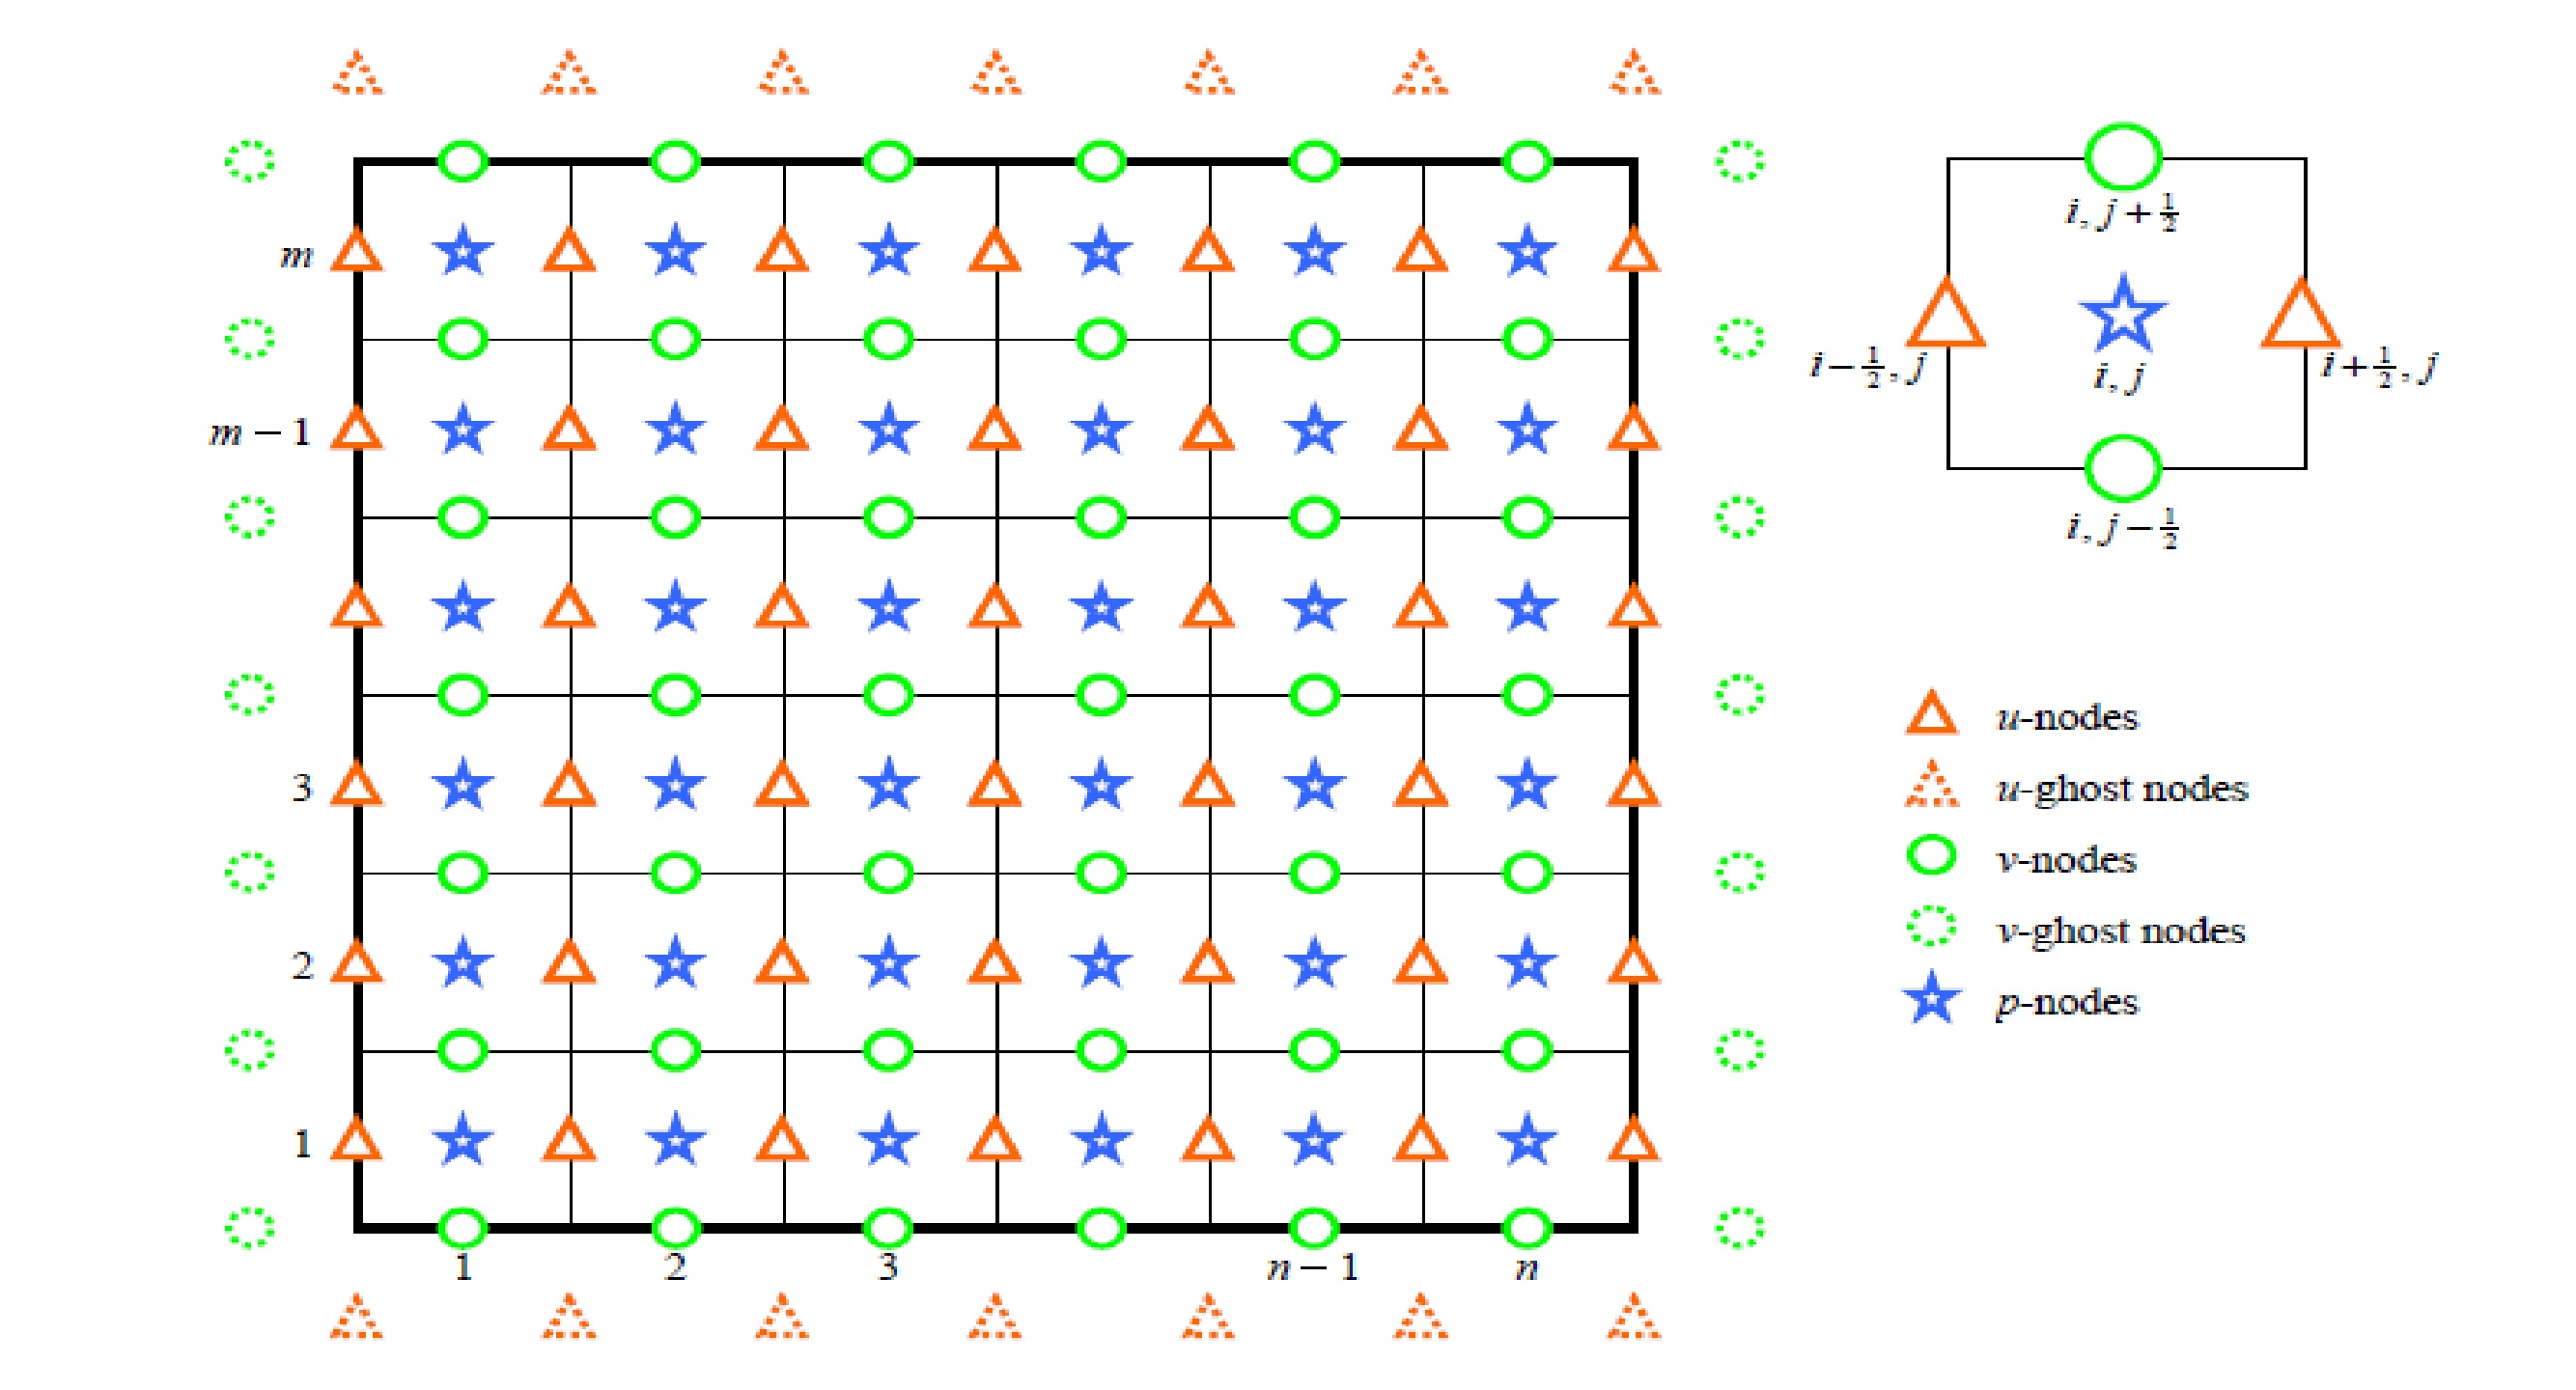
\includegraphics[width=6.5in]{C:/Users/HONGJI/Latex Home directory/staggered_grid.jpg}
	\caption{Picture of 2-D Staggered grid}\label{fig:6.1}
\end{figure}
The blue stars represents the pressure locations and corresponds to the indexing of $i = 1,2,3,\cdots n$ and $j = 1,2,3,\cdots m$; the red triangles are the ``horizontal" $u$ velocities have half indices and corresponds to $i-1/2 = 1/2, 3/2, \cdots n+1-1/2$ and $j=1,2,3,\cdots m$; the ``vertical" $v$ velocities also have half indices and corresponds to $i = 1,2,3,\cdots, n$ and $j-1/2 = 1/2, 3/2, \cdots m+1-1/2$. The boundary points are those stored at the edge of the domain. For instance, the $u$ velocities have west and east boundary points with indices of West: ($i=1/2,j$) and East: ($i=n+1/2,j$); $v$ velocities have North and South boundaries points with ($i,j=1/2$) and ($i,j=m+1/2$); whereas pressure only have interior points.\\

The derivatives can be calculated nicely in interior points however it is less straightforward to do so at the boundary points. For instance, if we want to know $\partial_y u_{i-1/2,1}$ next to the South boundary then this involves the up and down $u$ values with index $i-1/2,0$ and $i=3/2,2$. However $u_{i-1/2,0}$ simply does not exists because it is outside our domain. Can we ignore it? obviously not because it is needed to calculate derivatives. The inability to specify boundary values is one of the major drawbacks of staggered mesh grids. To tackle this problem, many people have used the concept of ``ghost cells" where we give $u$ a value at location ($-1/2,j$). Then the derivative operations can be conducted as normal as the interior points. Therefore interpolation is needed. Commonly, people have used 2 point average to calculate $u_{-1/2,j}$. However this only gives first order accuracy and degrades the global spatial convergence error. To avoid this, higher order interpolations are needed. Robert has used a cubic polynomial interpolation to guarantee second order accuracy all the way up the boundary \textbf{citation of Roberts report}. The formula can be derived by using Taylor expansion of 3 interior points and the ghost cell at the boundary point. Then after rearrangement and cancelling of other function derivatives we obtain:
\begin{equation}
u_{i-1/2,0} = \dfrac{16}{5} u_{i-1/2,1/2} - 3 u_{i-1/2,1} + u_{i-1/2,2} - \dfrac{1}{5}u_{i-1/2,3}
\end{equation}
The value at the corner e.g. $u_{i-1/2,1/2}$ are boundary values which will be given by the Dirichlet boundary condition for $u$.\\

The North counterpart is calculated similarly:
\begin{equation}
u_{i-1/2,m+1} = \dfrac{16}{5} u_{i-1/2,m+1/2} - 3 u_{i-1/2,m} + u_{i-1/2,m-1} - \dfrac{1}{5}u_{i-1/2,m-2}
\end{equation}
Similarly the $v$ velocities also suffer from this problem near the West and East boundaries and cubic interpolation is also used to calculate the ghost cells:
\begin{equation}
v_{0,j-1/2} = \dfrac{16}{5} u_{1/2,j-1/2} - 3 u_{1,j-1/2} + u_{2,j-1/2} - \dfrac{1}{5}u_{3,j-1/2}
\end{equation}
\begin{equation}
v_{n+1,j-1/2} = \dfrac{16}{5} u_{n+1/2,j-1/2} - 3 u_{n,j-1/2} + u_{n-1,j-1/2} - \dfrac{1}{5}u_{n-2,j-1/2}
\end{equation}

In Python, however we cannot work with ``half indices". Therefore a special treatment of index is needed. For instance, we can double the index values ($i \Rightarrow 2i,\,j \Rightarrow 2j$) so that half indices can be used. In our case, for the sake of simplicity, a re-indexing was used. Looking at the staggered grid again, by joining the triangles together (including ghost cells) we extract a grid for $u$ velocities. Then Python index can be used here. For instance, West corresponds to ($i=1/2,j$) in staggered grid now have index ($i=0,j$) in our new grid. Same strategy is used for $v$ and pressure too. It is worth to point out that the North and South are flipped between the staggered grid and Python grid.

\subsection{Discretisation of Convective and Diffusive terms}
Because for centered differencing, we want to calculate all of our variables ($u,\,v$ and $p$) at half time indices. Therefore a temporal discretisation of convective and diffusive terms are also needed.\\

An explicit second order Adam Bashforth scheme is used to discretise the Convective term $\left[(\textbf{u}\cdot\nabla)\textbf{u}\right]^{k+1/2}$. Here $k$ is used as time iterations.
\begin{equation}
\left[(\textbf{u}\cdot\nabla)\textbf{u}\right]^{k+1/2} = \dfrac{3}{2}\left[(\textbf{u}\cdot\nabla)\textbf{u}\right]^k - \dfrac{1}{2}\left[(\textbf{u}\cdot\nabla)\textbf{u}\right]^{k-1}
\end{equation}
The spatial discretisation follows from our first subsection with a change of indices to fit with the staggered mesh grid.\\
For $u$ velocities which live on the triangles
\begin{dgroup}
\begin{dmath}
\left[(\textbf{u}\cdot\nabla)\textbf{u}\right]_{i-1/2,j} = u_{i-1/2,j}\,\dfrac{\partial u_{i-1/2,j}}{\partial x} + v_{i-1/2,j}\,\dfrac{\partial u_{i-1/2,j}}{\partial y}
= u_{i-1/2,j}\,\dfrac{u_{i+1/2,j} - u_{i-3/2,j}}{2\Delta x} + v_{i-1/2,j}\,\dfrac{u_{i-1/2,j+1} - u_{i-1/2,j-1}}{2\Delta x}
\end{dmath}
\intertext{\\
However because in staggered grid, $v$ and $u$ are stored at different locations and hence spatial interpolation is again needed to compute $v_{i-1/2,j}$. This time a 4 point average will suffice for second order accuracy.\\
}
\begin{dmath*}
v_{i-1/2,j} = \dfrac{v_{i,j+1/2}+v_{i-1,j+1/2}+v_{i,j-1/2}+v_{i-1,j-1/2}}{4}
\end{dmath*}
\intertext{\\
Similarly for the $v$ component:
\\}
\begin{dmath}
\textbf{v}\cdot\nabla)\textbf{v})_{i,j-1/2} = u_{i,j-1/2}\,\dfrac{\partial v_{i,j-1/2}}{\partial x} + v_{i-1/2,j}\,\dfrac{\partial v_{i,j-1/2}}{\partial y}
= u_{i,j-1/2}\,\dfrac{v_{i+1,j-1/2} - v_{i-1,j-1/2}}{2\Delta x} + v_{i,j-1/2}\,\dfrac{v_{i,j+1/2} - v_{i,j-3/2}}{2\Delta x}
\end{dmath}
\intertext{\\
Once again 4 point average is used to compute $u_{i,j-1/2}$ which we do not have access to first.
\\}
\begin{dmath*}
v_{i,j-1/2} = \dfrac{v_{i-1/2,j}+v_{i+1,j}+v_{i+1,j-1}+v_{i-1,j-1}}{4}
\end{dmath*}
\end{dgroup}
There are other ways to treat the linear convective terms. We can put it into conservation form and use upwind scheme.

Crank Nicholson is used to treat the diffusive terms.
\begin{equation}
\nabla^2 \textbf{u}^{k+1/2} = \nabla^2\,(\textbf{u}^*+\textbf{u}^k)
\end{equation}
where $\nabla^2 \textbf{u}$ is discretised as
\begin{dgroup}
\begin{equation}
\nabla^2 u = \dfrac{u_{i+1/2,j} - 2u_{i-1/2,j}+u_{i-3/2,j}}{\Delta x^2}+\dfrac{u_{i-1/2,j+1} - 2u_{i-1/2,j}+u_{i-1/2,j-1}}{\Delta y^2}
\end{equation}
\begin{dmath}
\nabla^2 v = \dfrac{v_{i+1,j-1/2} - 2v_{i,j-1/2}+v_{i-1,j-1/2}}{\Delta x^2}+\dfrac{v_{i,j+1/2} - 2v_{i,j-1/2}+_{i,j-3/2}}{\Delta y^2}
\end{dmath}
\end{dgroup}

the divergence of velocity is a scalar field and hence needs to match up with the locations of pressure cells. it is calculated as:
\begin{equation}
\nabla \cdot \textbf{u}_{i,j} = \dfrac{u_{i+1/2,j} - u_{i-1/2,j}}{\Delta x} + \dfrac{v_{i,j+1/2} - v_{i,j-1/2}}{\Delta y}
\end{equation}

The gradient of pressure on the other hand is a vector field and hence needs to match up with the locations of velocities (triangles and circles). Hence it is calculated as follows:\\
x component:
\begin{dgroup}
\begin{dmath}
\partial_x p_{i-1/2,j} = \dfrac{p_{i,j} - p_{i-1,j}}{\Delta x}
\end{dmath}
\begin{dmath}
\partial_y p_{i,j-1/2} = \dfrac{p_{i,j} - p_{i,j-1}}{\Delta y}
\end{dmath}
\end{dgroup}

\subsection{Linear system solvers}
Now with every individual terms fully discretised and the introduction of intermediate velocity fields the momentum equation becomes:
\begin{equation}
\dfrac{\textbf{u}^* - \textbf{u}^n}{\Delta t} = -\nabla p^{n-1/2} -\dfrac{3}{2}\left[(\textbf{u}\cdot\nabla)\textbf{u}\right]^k + \dfrac{1}{2}\left[(\textbf{u}\cdot\nabla)\textbf{u}\right]^{k-1} + \dfrac{1}{2R}(\textbf{u}^*+\textbf{u}^n) + F^{n+1/2}
\end{equation}
where $F^{n+1/2}$ represents the external forcing, e.g. gravity.\\
Because we are working with $Pm\,1\,(b)$, hence we have taken the pressure approximation $q = p^{n-1/2}$.\\

Because of the implicit treat of diffusive terms, the intermediate velocity field must be solved as a linear system.\\
Further rearrange the momentum equation:
\begin{equation}
\left(I - \dfrac{\Delta t}{2R}\nabla^2\right)\textbf{u}^* = \textbf{u}^n + \Delta t\left(-\nabla p^{n-1/2} -\dfrac{3}{2}\left[(\textbf{u}\cdot\nabla)\textbf{u}\right]^k + \dfrac{1}{2}\left[(\textbf{u}\cdot\nabla)\textbf{u}\right]^{k-1} + \dfrac{1}{2R}(\textbf{u}^*+\textbf{u}^n) + F^{n+1/2} \right)
\end{equation}
Now with the Laplacian fully discretised, the problem above is a linear system to solve:
\begin{equation}
A\textbf{u}^* = \textbf{b}
\end{equation}
where $A = \left(I - \dfrac{\Delta t}{2R}\nabla^2\right)$ and $\textbf{b}$ equals to the right hand side of the above equation.\\

We use Algebraic multi-grid method provided in Scipy to solve it.\\

Poisson pressure.\\
This is directly resulted from projection:
\begin{equation}
\nabla^2 p = \dfrac{1}{\Delta t}\nabla \cdot \textbf{u}^*
\end{equation}
with boundary condition:
\begin{equation}
\textbf{n} \cdot \nabla p = 0
\end{equation}
\textbf{Normalisation approach.}\\
This Poisson equation is also solved by AMG multi-grid method. However care must be taken as the above equation wit the Neumann boundary condition gives unique solution of $\phi$ only up to the addition of a constant. Hence we must find a way to recover the exact solution. We basically needs to put an extra constraint into it.\\

We call this new modified approach as ``Pressure normalisation".\\

Although not discussed in the literature of Projection methods, we infer that a normalisation process is also implemented in the literature by researchers.\\

There are many choices of normalisation. One common one is forcing the $\phi$ to satisfies an integral constraint:
\begin{equation}
\int_{\Omega}\,\int_{\Omega}\,\phi \,\,\, dx dy = 0
\end{equation}
\textbf{Is this right?}
However this approach involves calculating integrals and due to the limited timing we did not use it. This could be done in future researches.\\

Setting 
\begin{equation}
\phi^{n+1}_{nu} = \phi^{n+1}_{ex} + a
\end{equation}
where the subscripts ``nu" and ``ex" stands for numerical and exact solutions respectivelyBecause of non-uniqueness there is no ``exact" $\phi$ solution, here exact refers to the one required by the projection method. Other $\phi$ solutions would causing the pressure to converge differently as we have seen before.\\

In practice $\phi^{n+1}_{nu}$ is first solved using the Poisson equation with the zero Neumann boundary condition\\

Because the Poisson equation with Neumann boundary condition does not guarantee uniqueness of $\phi$, hence we need to think what other constraints it must satisfy in the projection methods. In turns out that $\phi$ satisfies the pressure update equation! Rearrange equation (11) we obtain an expression for the constant $a$:
\begin{equation}
a = \phi^{n+1}_{nu} - \dfrac{1}{Re} \nabla \cdot \textbf{u}^* + (p^{n+1/2} - p^{n-1/2})
\end{equation}

This requires the knowledge of $p^{n+1/2}$ which of course we don't have when solving for $\phi^{n+1}$! However remember that $a$ is just a constant added to $\phi$ (and pressure), hence if we know the the pressure field at one point in domain then we can fully recover $a$. This point is arbitrary, but in practice, it is usually chosen along the boundary or center or any other points easily accessed. Therefore we need to impose a ``partial" Dirichlet condition on pressure. It is partial because we only require the knowledge of point in space. In this section, we have chosen the point from the boundary.

\begin{equation}
a = \phi^{n+1}_{nu}\,(x,y)|_{(x,y)\in \partial\Omega} \,\,\,-\,\,\, \dfrac{1}{Re} \nabla \cdot \textbf{u}^*\,(x,y)|_{(x,y)\in \partial\Omega}\,\,\, +\,\,\, (p^{n+1/2} - p^{n-1/2})\,(x,y)|_{(x,y)\in \partial\Omega}
\end{equation}

Practically in order to ensure consistency we take 2 to 4 points along each boundary or corner and taking their average. \\

For the forced flow example we are considering, the analytical solution ($p = \sin(t)\cos(\pi x)\sin(\pi y)$) indicates the North and South boundaries ($y=\pm 1$) are essentially zero for domain $[-1,1]^2$. Therefore naturally one can consider inhomogeneous Dirichlet boundary condition for pressure variable. Then by picking one arbitrary point along the boundary (for instance $y=1$ and $x$ is arbitrary) our equation for $c$ reads:
\begin{equation*}
a = \phi^{n+1}_{nu}\,(x,1) \,\,\,-\,\,\, \dfrac{1}{Re} \nabla \cdot \textbf{u}^*\,(x,1)
\end{equation*}
In the case of Staggered grids the spatial point $(x,1)$ corresponds to an index of $i, \, j = \dfrac{1}{2}$ where $i$ stands for the horizontal index and $j$ the vertical index. Dropping the time index for convenience we obtain:
\begin{equation*}
a = \phi^{nu}_{i,\,1/2} \,\,\,-\,\,\, \dfrac{1}{Re} \nabla \cdot \textbf{u}^*_{i,\,1/2}
\end{equation*}

However in Staggered grids, the coordinate ($i,\,1/2$) is along the top edge of the grid and no pressure is stored at this point (pressure is stored at ($i,\,j$) locations). Therefore interpolation from nearby cells are needed. This introduces spatial interpolation error and hence care must be taken to avoid accumulation of spatial errors.\\

In this case, we use a 3rd order cubic interpolation for $\phi^{nu}_{i,\,1/2}$ from 3 nearby points: $\phi^{nu}_{i,\,1}$, $\phi^{nu}_{i,\,2}$ and $\phi^{nu}_{i,\,3}$. Cubic interpolation is needed to ensure the first order derivative of $\phi^{nu}_{i,\,1/2}$ is also second order accurate along the boundary.\\
We Taylor expand $\phi^{nu}_{i,\,1}$, $\phi^{nu}_{i,\,2}$ and $\phi^{nu}_{i,\,3}$ at location ($i,\,1/2$) up to order $\mathcal{O}(\Delta t^3)$ and we obtained an interpolation formula for $\phi^{nu}_{i,\,1/2}$ as

\begin{equation}
\phi^{nu}_{i,\,1/2} = \dfrac{15}{8}_{i,1} - \dfrac{5}{4}_{i,\,2}+\dfrac{3}{8}_{i,\,3}
\end{equation}
Exactly the formula can be used for $\nabla \cdot \textbf{u}^*$ since they are stored at the same locations as $\phi$.\\

Then the exact $\phi^{n+1}$ can thus be obtained by subtracting $c$ from $\phi^{n+1}_{nu}$ point-wisely. Thus we minus the same constant $a$ on every point of $\phi^{nu}$. Then the correct pressure can be recovered and we call it the ``Normalised Pressure". This in theory should fix the problem of error of error enlargement at finer grids. And this method indeed works as we shall shortly!\\

For Projection method $Pm\,2$, exactly the process is used. In fact the expression for $c$ is identical.\\

For Gauge method, exactly the same procedure can be implemented too. From solving the Poisson equation we know that:
\begin{equation}
\chi^{n+1}_{nu} = \chi^{n+1}_{ex} + b\,\,\,\text{ and }\,\,\,\chi^{n}_{n} = \chi^n_{ex} + c
\end{equation}
where $b$ and $c$ are constants. They are generally not equal and hence Gauge method also suffers from the non-uniqueness problem.\\

Again the point where we evaluate $b$ and $c$ is arbitrary, so let's use the same one considered above.\\
Substitute the expression of $\chi_{nu}$ into the pressure update equation and rearranging we obtain:
\begin{equation}
b - c = \chi^{n+1,\,\,\,nu}_{i,\,1/2} - \chi^{n,\,\,\,nu}_{i,\,1/2} + \dfrac{\Delta t}{2\,Re}(\nabla \cdot m^{n+1}_{i,\,1/2} + \nabla \cdot m^n_{i,\,1/2})
\end{equation}

\subsection{update velocity and pressure.}
This is the easiest step:\\
The velocities are updated as follows:\\
By projection step:\\
new $u$ velocity:
\begin{dgroup}
\begin{dmath}
u^{k+1}_{i-1/2,j} = u^*_{i-1/2,j} - \Delta t \partial_x p_{i-1/2,j} = u^*_{i-1/2,j} - \Delta t \,\dfrac{p_{i,j} - p_{i-1,j}}{\Delta x}
\end{dmath}
\intertext{and new $v$ velocity}
\begin{dmath}
v^{k+1}_{i,j-1/2} = u^*_{i,j-1/2} - \Delta t \partial_y p_{i,j-1/2} = u^*_{i,j-1/2} - \Delta t \,\dfrac{p_{i,j} - p_{i,j-1}}{\Delta y}
\end{dmath}
\end{dgroup}

and finally pressure:
\begin{equation}
p^{n+1/2}_{i,j} = p^{n-1/2}_{i,j} + \phi^{n+1}_{i,j} - \dfrac{\Delta t}{2R}\nabla^2\phi^{n+1}_{i,j} = p^{n-1/2}_{i,j} + \phi^{n+1}_{i,j} - \dfrac{1}{2R}\nabla \cdot \textbf{u}^*_{i,j}
\end{equation}
  \chapter{Numerical Results}
\label{chapter 6}
In this chapter, we present the results generated by our numerical solvers based on projection methods: Alg 1, Alg 2 and Alg 3, as well as the Gauge method. We investigate each method's accuracy through numerical tests and visual simulations.

\section*{Numerical validation of Projection methods}
\section{Accuracy test}
There are many ways to test the accuracy of numerical schemes. One of the most popular way is to compare the numerical solutions generated through computer simulations with analytical solutions. By calculating the error with appropriate norms (e.g. $L_1,\,L_2$ and $L_\infty$) this method provides precise measure on error and convergence rate. In case where analytical solutions are not known or difficult to implement, people often use bench mark results. These results are not the analytical solutions to the test problem, rather they are numerical solutions generated in fine grids that are widely accepted in literature. For instance, the lid driven cavity problem is such a simple test problem which shows turbulent flow patterns. We will give a qualitative illustration of the classic cavity problem in this chapter too.

For the main part of this chapter because we are aiming to conduct accuracy and convergence test of projection methods, hence we consider two simple 2-D flow problems where analytic solutions do exist. This reveals more fundamental properties and error behaviours for the projection schemes.\\

\subsection{Forced flow}
The test problem is a forced flow example where the fluid is confined in a square domain $\Omega = [-1,1] \times [-1,1]$ and initially remains stationary. The flow is initiated by an external driving force. This is one of the simplest settings to consider slip/no-slip boundary conditions. In this case an homogeneous boundary condition (no - slip) is imposed on the four sides of the domain \\
($\partial \Omega:$ West: $x = -1$, East: $x=1$, South: $y = -1$, North: $y=1$).\\

The analytical solution satisfies:
\begin{equation}
\begin{cases}
u = \pi\sin(t)\sin(2\pi y)\sin^2(\pi x) \text{   in $\Omega$} \\
v = - \pi \sin(t)\sin(2\pi x)\sin^2(\pi y) \text{   in $\Omega$} \\
p = \sin(t)\cos(\pi x)\sin(\pi y)  \text{   in $\Omega$}  \\
u_0 = u(t=0,x,y)  \text{   in $\Omega$}  \\
v_0 = v(t=0,x,y)  \text{   in $\Omega$}  \\
\end{cases}
\end{equation}
with homogeneous Dirichlet boundary condition:
\begin{equation*}
u(t, x=\pm 1, y) = v(t, x,y= \pm 1) = 0
\end{equation*}

It is augmented with a forcing term: $f = \partial_t\,\textbf{u} - \dfrac{1}{R}\nabla^2 \textbf{u} + \nabla p$ to make the above ``solutions" valid. For simplicity we take the Reynolds number ($R$) to be 1. By substituting our analytical solutions into $f$ we find the forcing term is:
\begin{equation}
f = 
\begin{cases}
fx = \pi\cos(t)\sin(2\pi y)\sin^2(\pi x) -  2 \pi^3\sin(t)\sin(2\pi y)\,(\cos(2\pi x) - 2\sin^2(\pi x)) \\
\,\,\,\,\,\,\,- \, \pi\sin(t)\sin(\pi y)\sin(\pi x) \text{   in $\Omega$} \\
fy = - \pi\cos(t)\sin(2\pi x)\sin^2(\pi y) - 2\pi^3\sin(t)\sin(2\pi x)\,(2\sin^2(\pi y) - \cos(2\pi y)) \\
\,\,\,\,\,\,\,+ \, \pi\sin(t)\cos(\pi x)\cos(\pi y)  \text{   in $\Omega$}  \\
\end{cases}
\end{equation}

The CFL number is given as: $CFL = U\,\Delta t/\Delta x$ where $U = \pi$ is the absolute bound for velocity. We want the CFL number to be below one to ensure stability. However too small CFL number will decrease the efficiency because the numerical solver would take a longer time to run to incorporate small time stepping. Hence we have chosen the optimal CFL number to be 0.5. This is also a commonly used value \cite{brown2001accurate}.

The actual error $e_h$ is consisted of both spatial and temporal error and $h$ is just an index to indicate the grid size (e.g. a 120 $\times$ 120 grid).\\
In our purpose of testing the temporal error behaviour, we want the temporal error to dominate and thus we can assume the following simplified error relation:
\begin{equation}
e_h = \Delta t^p
\end{equation}
where $p$ is the convergence rate or order of accuracy (don't be confused with pressure) and in our case we want $p=2$.\\

The error $e_h$ is simply calculated by taking the difference between numerical and analytical solutions point-wisely. It is important to compare the solutions only under the same conditions, for instance sane grid sizes and end of time... Comparing solutions at different time would of course cause strange error behaviours!\\

By taking the logarithm on both side of the equation above we see that the logarithm of error in time has a linear relationship with the logarithm of time stepping ($\Delta t$). Thus the slope of the log error function should be the convergence rate $p$.
\begin{equation}
\log_{10} (e_h) = p\log_{10} (\Delta t)
\end{equation}
Base 10 is used for simplicity, other bases including 2 and natural exponential works the same.\\

The strategy is follows: with the error of a coarse grid denoted as $e_h$. We half the spatial stepping ($\Delta x$) or equivalently double the grid size (e.g. from 15 $\times$ 15 to 30 $\times$ 30). Denoting the error of the finer grid as $e_{h_{1/2}}$. The time stepping mean while is also halved. Then we look at how the error decreases. If our numerical scheme is second order accurate then the error should decrease by a factor of 4 going from the coarser grid to finer grid.\\

A Log-Log plot of the error function is then generated and the convergence rate is finally extracted as the slope of the log error function.\\

It is important to specify the error norm. As noted by many researchers that different norms could generated different convergence rates! \cite{pyo2005normal,guermond2004error}\\
In our analysis 3 commonly used norms were implemented: $L_1,\,L_2$ and $L_\infty$. Each could reveal certain aspect of error behaviour. By combing the results using these 3 norms, a comprehensive analysis of convergence rate can be obtained.\\

We take the normalised $L_1$ norm and it is defined as:
\begin{equation}
||\,e^n\,||_{L_1} = \dfrac{1}{M}\,\sum^M_{m=0}\,|e^n_m|
\end{equation} 
where $e^n$ is the error field measured at time iteration $n$ and $M$ is the dimension or size of the error field. For instance a $15 \times 15$ grid corresponds to $M = 15^2$.\\

similarly we define the $L_2$ norm to be:
\begin{equation}
||\,e^n\,||_{L_2} = \left(\dfrac{1}{M^2}\,\sum^M_{m=0}\,|e^n_m|^2\right)^{1/2} = \dfrac{1}{M}\left(\sum^M_{m=0}\,|e^n_m|^2\right)^{1/2}
\end{equation}

and $L_\infty$:
\begin{equation}
||\,e^n\,||_{L_\infty} = \max_{\,\,\,0 \leq m \leq M\,\,\,}\,|e^n_m|
\end{equation}

To achieve optimal results, there are a number of things that need to be considered. \\
First, since we are aiming to investigate the temporal error and hence we need to use fine grids (small spatial stepping: $\Delta x <<1$) to ensure the spatial error is negligible. Formally we want: $\Delta x^2 << \dfrac{1}{R}\Delta t$. Hence we have run the solvers up to a grid size of $240 \times 240$ and also $480 \times 480$ sometimes. Higher grid numbers are also possible but takes very long time to compute, which would decrease the efficiency. For completeness we have also included the results for small to moderate grids. Overall we have maximum 6 data points corresponding to grid size of 15, 30, 60, 120, 240 and 480.\\

Second, care must also be taken to the pressure gradient along the boundary. We need to make sure the normal pressure gradient is non-zero along the boundary so that the accuracy performance can be distinguished between projection method Alg 1 and Alg 2. Fortunately, for our forced flow solutions, the normal pressure gradient is non-zero along the North and South boundaries ($y = \pm 1$) (whereas it is zero along the other two boundaries).\\

With the above conditions all satisfied, we can now finally test our numerical solutions! As for a start, we run the simulations at $t = 1$ with the spatial domain: $[-1,1]^2$ and homogeneous Dirichlet boundary conditions imposed on velocities.\\

The exact and numerical solutions are summarised in Figure 6.1. The numerical solutions are computed by Alg 2 with grid size: $60 \times 60$ and $CFL = 0.5$. The numerical solutions seem to do a good job in approximating the true solutions. These ``nice" graphs however do not reveal much information about the error behaviours. Hence we need to look at the convergence rates instead.\\

We first compare Alg 1 and Alg 2 results to illustrate the improvement of modified pressure update formula (Equation 3.32 a) with $q = p^{n-1/2}$). The errors for grid size 30 to 120 are summarised in Table 1. In addition the convergence rates for both $U$ and $V$ velocities are highly identical, hence we only report the $U$ component results in the subsequent analysis. It is clear that the velocities in both Alg 1 and Alg 2 show second order convergence rates across all norms whereas in pressure they do not. For Alg 1, $L_1$ and $L_2$ norms show first order convergence rate (1.29 and 1.21 respectively) whereas $L_\infty$ shows an even deteriorated rate of 0.32. The sudden drop in convergence rate in $L_\infty$ indicates the presence of numerical boundary layer, because $L_\infty$ picks up the large errors or singularities better. \\
   For Alg 2, the results in pressure are better, but still not very satisfied. $L_1$ norm shows a close to second order rate of 1.92 whereas $L_2$ shows a decreased rate of about 1.74. The $L_\infty$ then further decreased to only about first order rate (1.14). The degradation of accuracy in $L_\infty$ also indicate the presence of large singularities, whereas $L_1,\,L_2$ tend to smooth them out. The overall magnitude of error is also relatively smaller in Alg 2. Take a look at the pressure error field in Figure 6.2, we found a pronounced numerical boundary layer in Alg 1 corresponding to $y = \pm 1$. Note that the normal gradient of pressure at these two boundaries is $\textbf{n}\cdot \nabla p |_{y = \pm 1} = \mp \pi \sin(t)\,\cos(\pi x) \neq 0$. Hence this indicates clearly the numerical boundary layer is very much formed by the inconsistent normal pressure gradient resulted from the old pressure updated formula used in Alg 1. In Alg 2 the numerical boundary layer seems still exists but reduced to four thinner spikes located at the corners of the domain. In addition, the magnitude of the boundary layer in Alg 2 is also about 4 times smaller. All these observations indicate that the modified pressure update formula in Alg 2 do seem to filter out the spurious mode contained in the intermediate velocity field and auxiliary field better, and hence gives better pressure error convergence. This is consistent with our predications in normal mode analysis and also matches with the findings from other researchers like David, Strikwerda and Shen et al \cite{brown2001accurate, strikwerda1999accuracy, guermond2006overview, guermond2004error}.\\

\begin{table}[H]
  \begin{center}
    \begin{tabular}{| l | c | c c c | r |}
    \hline
    Error in $U$ velocity \\
    \hline
    Alg 1 & Error norm & $30 \times 30$ & $60 \times 60$ & $120 \times 120$ & rates \\
     & $L_1$ & 3.75e-4 & 9.34e-5 & 2.32e-5 & 2.01 \\
     & $L_2$ & 4.66e-4 & 1.16e-4 & 1.88e-5 & 2.0 \\
     & $L_\infty$ & 1.11e-3 & 2.77e-4 & 6.89e-5 & 2.02\\
    \hline
    Alg 2
     & $L_1$ & 3.23e-4 & 8.01e-5 & 1.99e-5 & 2.01 \\
     & $L_2$ & 4.09e-4 & 1.01e-4 & 2.53e-5 & 2.00 \\
     & $L_\infty$ & 9.23e-4 & 2.33e-4 & 5.81e-5 & 2.00\\
    \hline
    \hline
    Error in Pressure\\
    \hline
    Alg 1 & Error norm & $30 \times 30$ & $60 \times 60$ & $120 \times 120$ & rates \\
     & $L_1$ & 6.96e-3 & 1.77e-3 & 7.29e-4 & 1.29 \\
     & $L_2$ & 1.02e-2 & 3.07e-3 & 1.33e-3 & 1.21 \\
     & $L_\infty$ & 6.64e-2 & 3.87-2 & 3.01e-3 & 0.32\\
    \hline
    Alg 2
     & $L_1$ & 1.26e-3 & 2.99e-4 & 8.32e-5 & 1.92 \\
     & $L_2$ & 1.68e-3 & 4.59e-4 & 1.47e-4 & 1.74 \\
     & $L_\infty$ & 9.36e-3 & 6.31e-3 & 3.24e-3 & 1.14\\
	\hline
    \end{tabular}
  \end{center}
  \caption{Error in $U$ velocity and pressure for Alg 1 and Alg 2, cfl = 0.5}
\end{table}

\begin{figure}[H]
	\centering
	\begin{subfigure}[t]{2.5in}
		\centering
		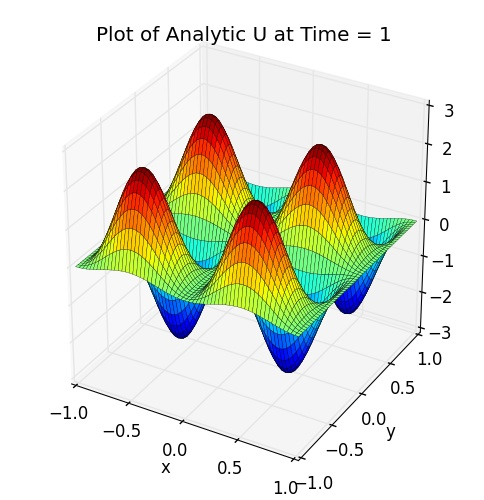
\includegraphics[width=2.5in]{C:/Users/HONGJI/Latex Home directory/Pm1a_pf2_U_exact_t_1_grid_60 - Copy.jpg}
		\caption{Analytic $U$ velocity at $t=1$}\label{fig:6.1a}		
	\end{subfigure}
	\quad
	\begin{subfigure}[t]{2.5in}
		\centering
		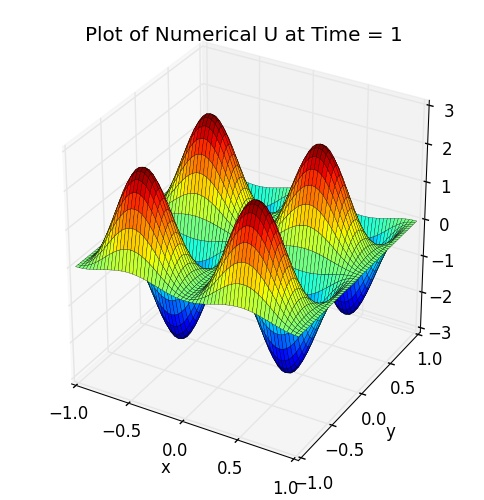
\includegraphics[width=2.5in]{C:/Users/HONGJI/Latex Home directory/Pm1a_pf2_uf_t_1_grid_60 - Copy.jpg}
		\caption{Numerical $U$ velocity at $t=1$}\label{fig:6.1b}
	\end{subfigure}
	\quad
	\begin{subfigure}[t]{2.5in}
		\centering
		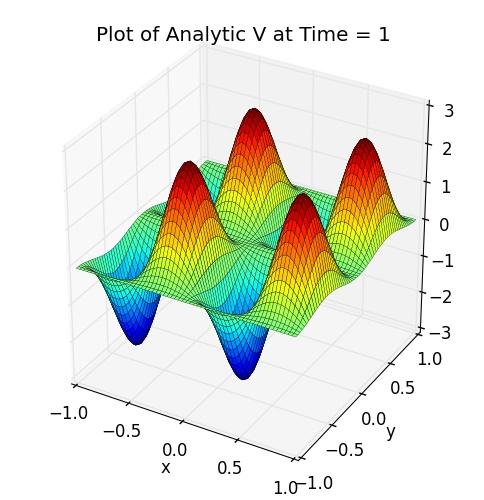
\includegraphics[width=2.5in]{C:/Users/HONGJI/Latex Home directory/Pm1a_pf2_V_exact_t_1_grid_60 - Copy.jpg}
		\caption{Analytic $V$ velocity at $t=1$}\label{fig:6.1c}
	\end{subfigure}
	\quad
	\begin{subfigure}[t]{2.5in}
		\centering
		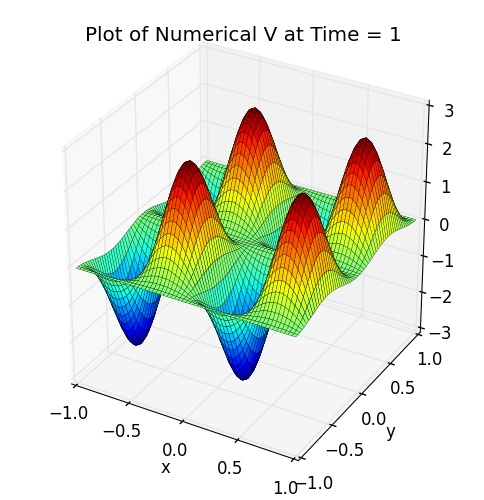
\includegraphics[width=2.5in]{C:/Users/HONGJI/Latex Home directory/Pm1a_pf2_vf_t_1_grid_60 - Copy.jpg}
		\caption{Numerical $V$ velocity at $t=1$}\label{fig:6.1d}
	\end{subfigure}
	\quad	
	\begin{subfigure}[t]{2.5in}
		\centering
		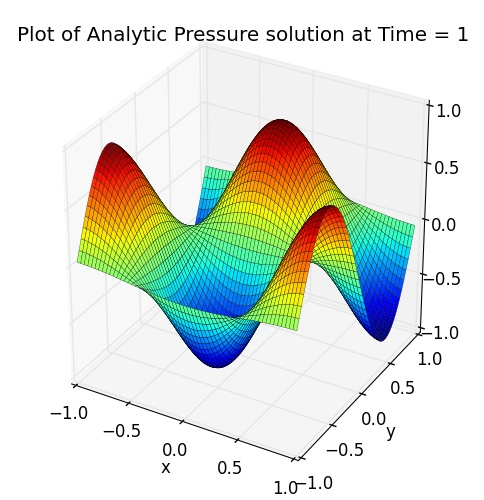
\includegraphics[width=2.5in]{C:/Users/HONGJI/Latex Home directory/Pm1a_pf2_P_exact_t_1_grid_60 - Copy.jpg}
		\caption{Analytic pressure ($P$) at $t=1$}\label{fig:6.1e}
	\end{subfigure}
	\quad	
	\begin{subfigure}[t]{2.5in}
		\centering
		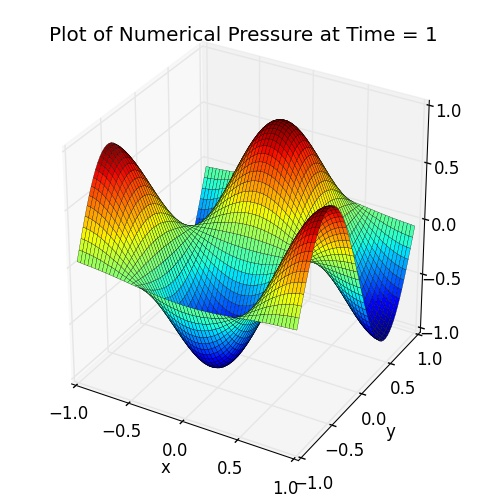
\includegraphics[width=2.5in]{C:/Users/HONGJI/Latex Home directory/Pm1a_pf2_pf_t_1_grid_60 - Copy.jpg}
		\caption{Numerical pressure ($P$) at $t=1$}\label{fig:6.1f}
	\end{subfigure}
	\caption{Plot of exact and numerical solutions ($U,V,P$) at time $t=1$ on the spatial domain of $[-1,1]^2$ with grid size $60 \times 60$, Alg 2 was used to compute the numerical solutions with $CFL=0.5$}\label{fig:6.1}
\end{figure}

\begin{figure}[H]
	\centering
	\begin{subfigure}[t]{2.5in}
		\centering
		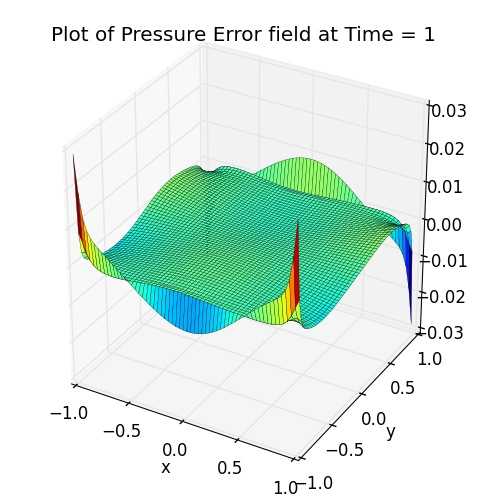
\includegraphics[width=2.5in]{C:/Users/HONGJI/Latex Home directory/Pm1a_pf2_P_error_t_1_grid_60_cfl_0_1.jpg}
		\caption{Pressure error field for Alg 1 at $t=1$ }\label{fig:6.2a}		
	\end{subfigure}
	\quad
	\begin{subfigure}[t]{2.5in}
		\centering
		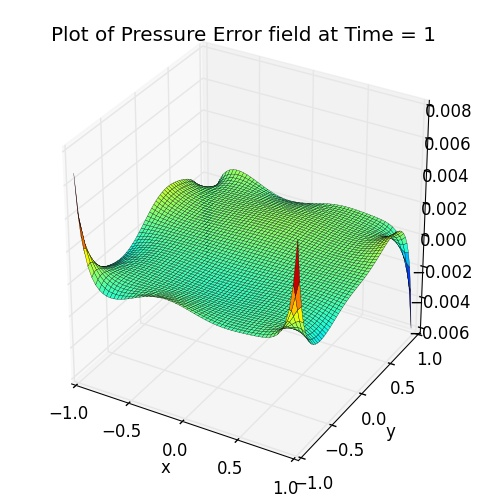
\includegraphics[width=2.5in]{C:/Users/HONGJI/Latex Home directory/Pm1b_pf2_P_error_t_1_grid_60_cfl_0_1.jpg}
		\caption{Pressure error field for Alg 2 at $t=1$}\label{fig:6.2b}
	\end{subfigure}
	\caption{$3D$ surface plot of pressure error field for Alg 1 and Alg 2 at time $t=1$ on the spatial domain of $[-1,1]^2$ with grid size $60 \times 60$ and $CFL=0.5$}\label{fig:6.2}
\end{figure}

We then compare with the schemes that were all predicated to be second order accurate, namely Alg 2, Alg 3 and Gauge method. The same test problem is used with the same domain ($[-1,1]^2$) and end time to ensure consistency. This time only the convergence in pressure error and divergence of intermediate velocity fields are shown because the convergence in velocities in all methods are consistently second order. We focus more on the error in pressure.\\

The Log-Log plot for errors in pressure are summarised below. We have run the code from $15 \times 15$ up to the $480 \times 480$ the finest. Even finer grids are also able to be calculated by increasing the number of cells, but this is omitted due to the exceedingly long hours take in solving the Poisson equations.\\

Interestingly we observe an outlier at grid size 15 where the pressure error is very large compared to the those at the finer grids. This is observed in all methods for this test problem. This is most likely due to the large spatial error which dominates at such a small grid size. Hence for the sake of reliability, we excluded these data points when computing the convergence rates. The errors after grid 60 reduces consistently and converge asymptotically to the second order reference slope (especially for Alg 3 and Gauge method). This asymptotic convergence behaviour is due to the gradual phasing out of spatial errors dominance at finer and finer grids. This is the most common error behaviour in Projection methods and our results now fully line up with those found in literature \cite{guermond2004error}. \\

Even though Alg 3 and Gauge methods show optimal 2nd order convergence for this test problem, the projection method Alg 1 however shows deprecated convergence especially measured in $L_\infty$. This is because the four spikes in the pressure error plot for Alg 2 before. The pressure error field for Alg 3 and Gauge method shows smooth boundary layers instead. Interestingly the convergence rates in $\nabla \cdot \textbf{u}^*$ is higher in Alg 2 than Alg 3 with about 1.5 to 1.8 order accuracy compared to 0.4 to 0.8 respectively. This is consistent with our hypothesis that the intermediate velocity field approximates the true velocity fields better in Alg 2. \\

Taking a look at the surface plot of $\nabla \cdot \textbf{u}^*$ in Figure 6.6 both methods shows the presence of numerical boundary layers because we know that $\nabla \cdot \textbf{u}^*$ contains the spurious mode ($e^{-\gamma x}$). Hence, our results indicate that the numerical boundary layer contained in the auxiliary variables in projection methods are better filtered out in Alg 3 than Alg 2. The exact cause of the deterioration in performance in Alg 2 still remains puzzling. Because both methods use the same pressure update formula, hence we infer that it is the boundary condition for $\textbf{u} ^*$ and pressure approximation which affects the performance. As discussed in the normal analysis chapter that we know that Alg 2 has an inconsistent normal pressure gradient resulted from the choice of pressure approximation $q$. When $q = p^{n-1/2}$ as in Alg 2 this is ``forcing" the normal pressure gradient at time $(n+1/2)\Delta t$ to be zero which is inconsistent with that of the analytic counterpart at boundary $y = \pm 1$. Then numerical boundary layer cannot be completely filtered out. However this explanation is not very satisfactory as the normal analytic pressure gradient is zero independent of time at boundaries $x = \pm 1$, but we clearly observes four spikes in each corner of the domain the pressure error plot. We will rather illustrate the inconsistent choice of $q$ in a different test problem. The problem is possibly not caused by boundary conditions choice of $\textbf{u}^*$ because we see a good convergence rate in $\nabla \cdot\textbf{u}^*$. \\

Taking a closer look at the the plot of the analytic pressure field, it seems like the pressure values rapidly to zero approaching the North and South boundaries at $y=\pm 1$. This implies large change in pressure gradients along boundary. We infer that the cubic spatial interpolation of ``ghost cells" implemented in a staggered grid solver causes the pressure gradients to have a sharp increase along boundary. Then combined with the inconsistent choice of $q$ we see a degradation of accuracy in pressure in Alg 2. As suggested by Brown (although a different test problem), the large numerical boundary layer problem in $\nabla \cdot\textbf{u}^*$ could be reduced by making velocity variables to satisfy a ``free boundary condition" where its third order derivative is zero. Then this might help to increase the convergence rate in pressure \cite{brown2001accurate}. However this is problem dependent and due to limited space and time we did not implement this.\\

\begin{figure}[H]
	\centering
	\begin{subfigure}[t]{4.5in}
		\centering
		\scalebox{1.2}{
		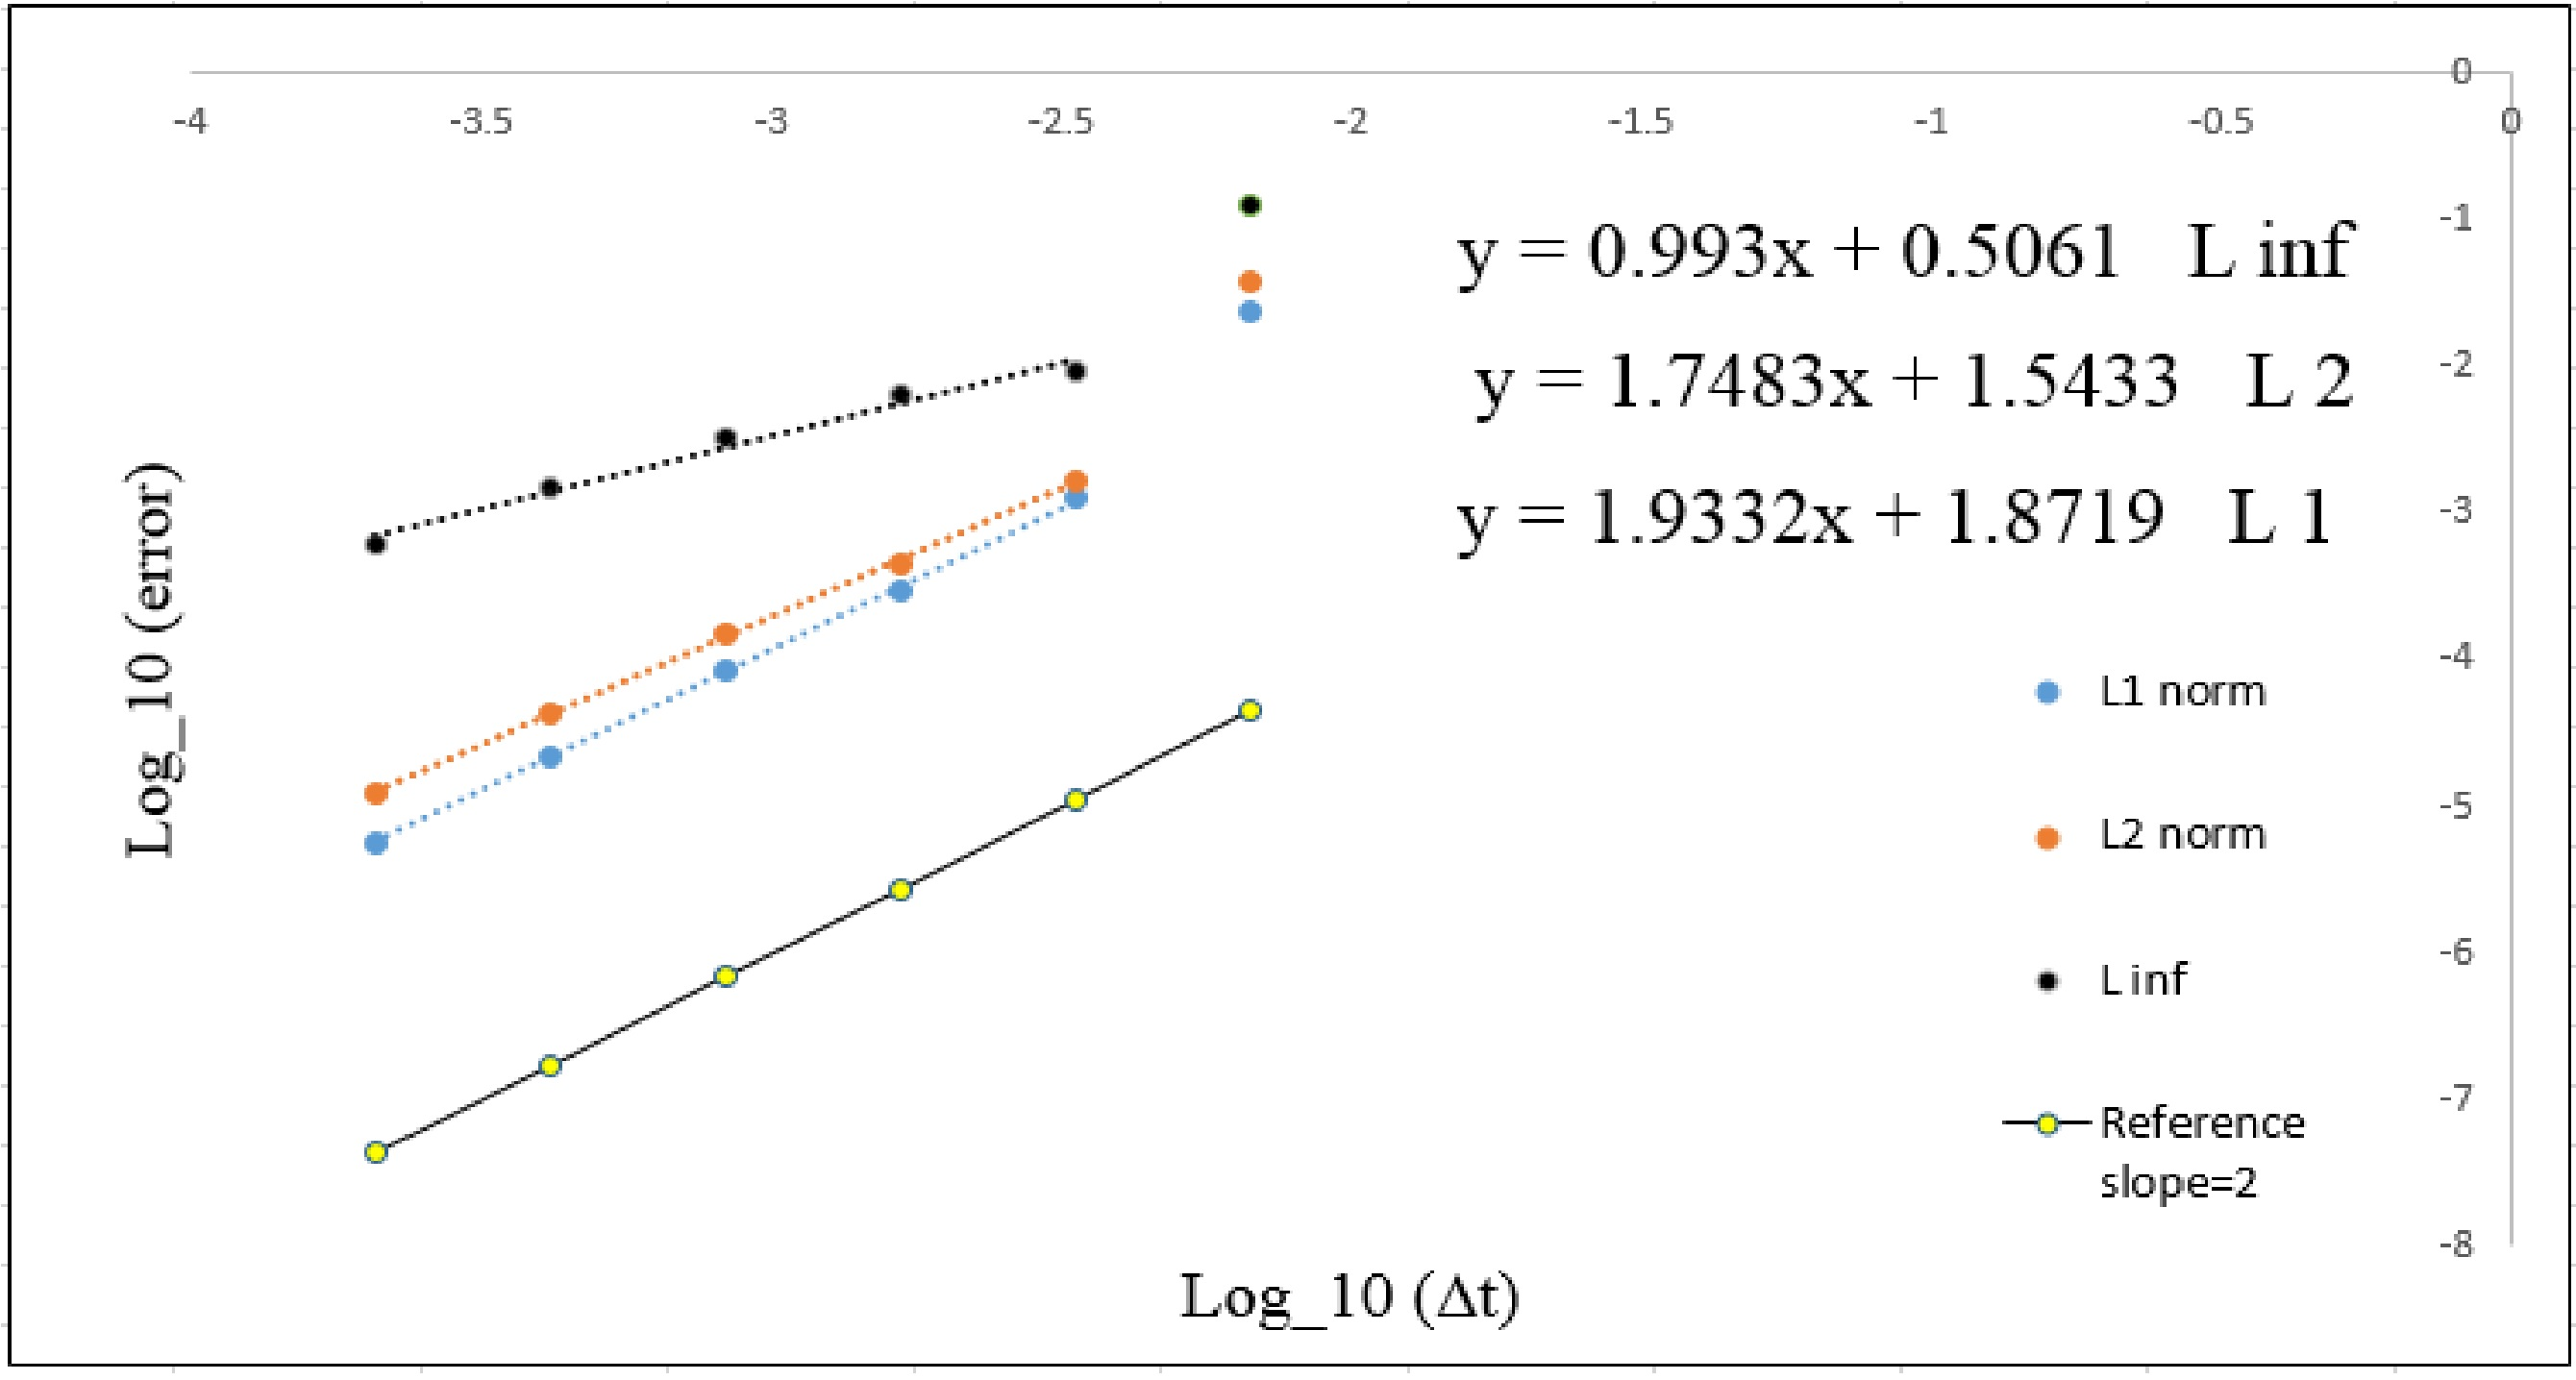
\includegraphics[width=4.5in]{C:/Users/HONGJI/Latex Home directory/Pm1b_pf2_np_P_rate_c_0_5.jpg}}
		\caption{Log-Log plot of Convergence rate for Pressure}\label{fig:6.19a}		
	\end{subfigure}
	\quad
	\begin{subfigure}[t]{4.5in}
		\centering
		\scalebox{1.2}{
		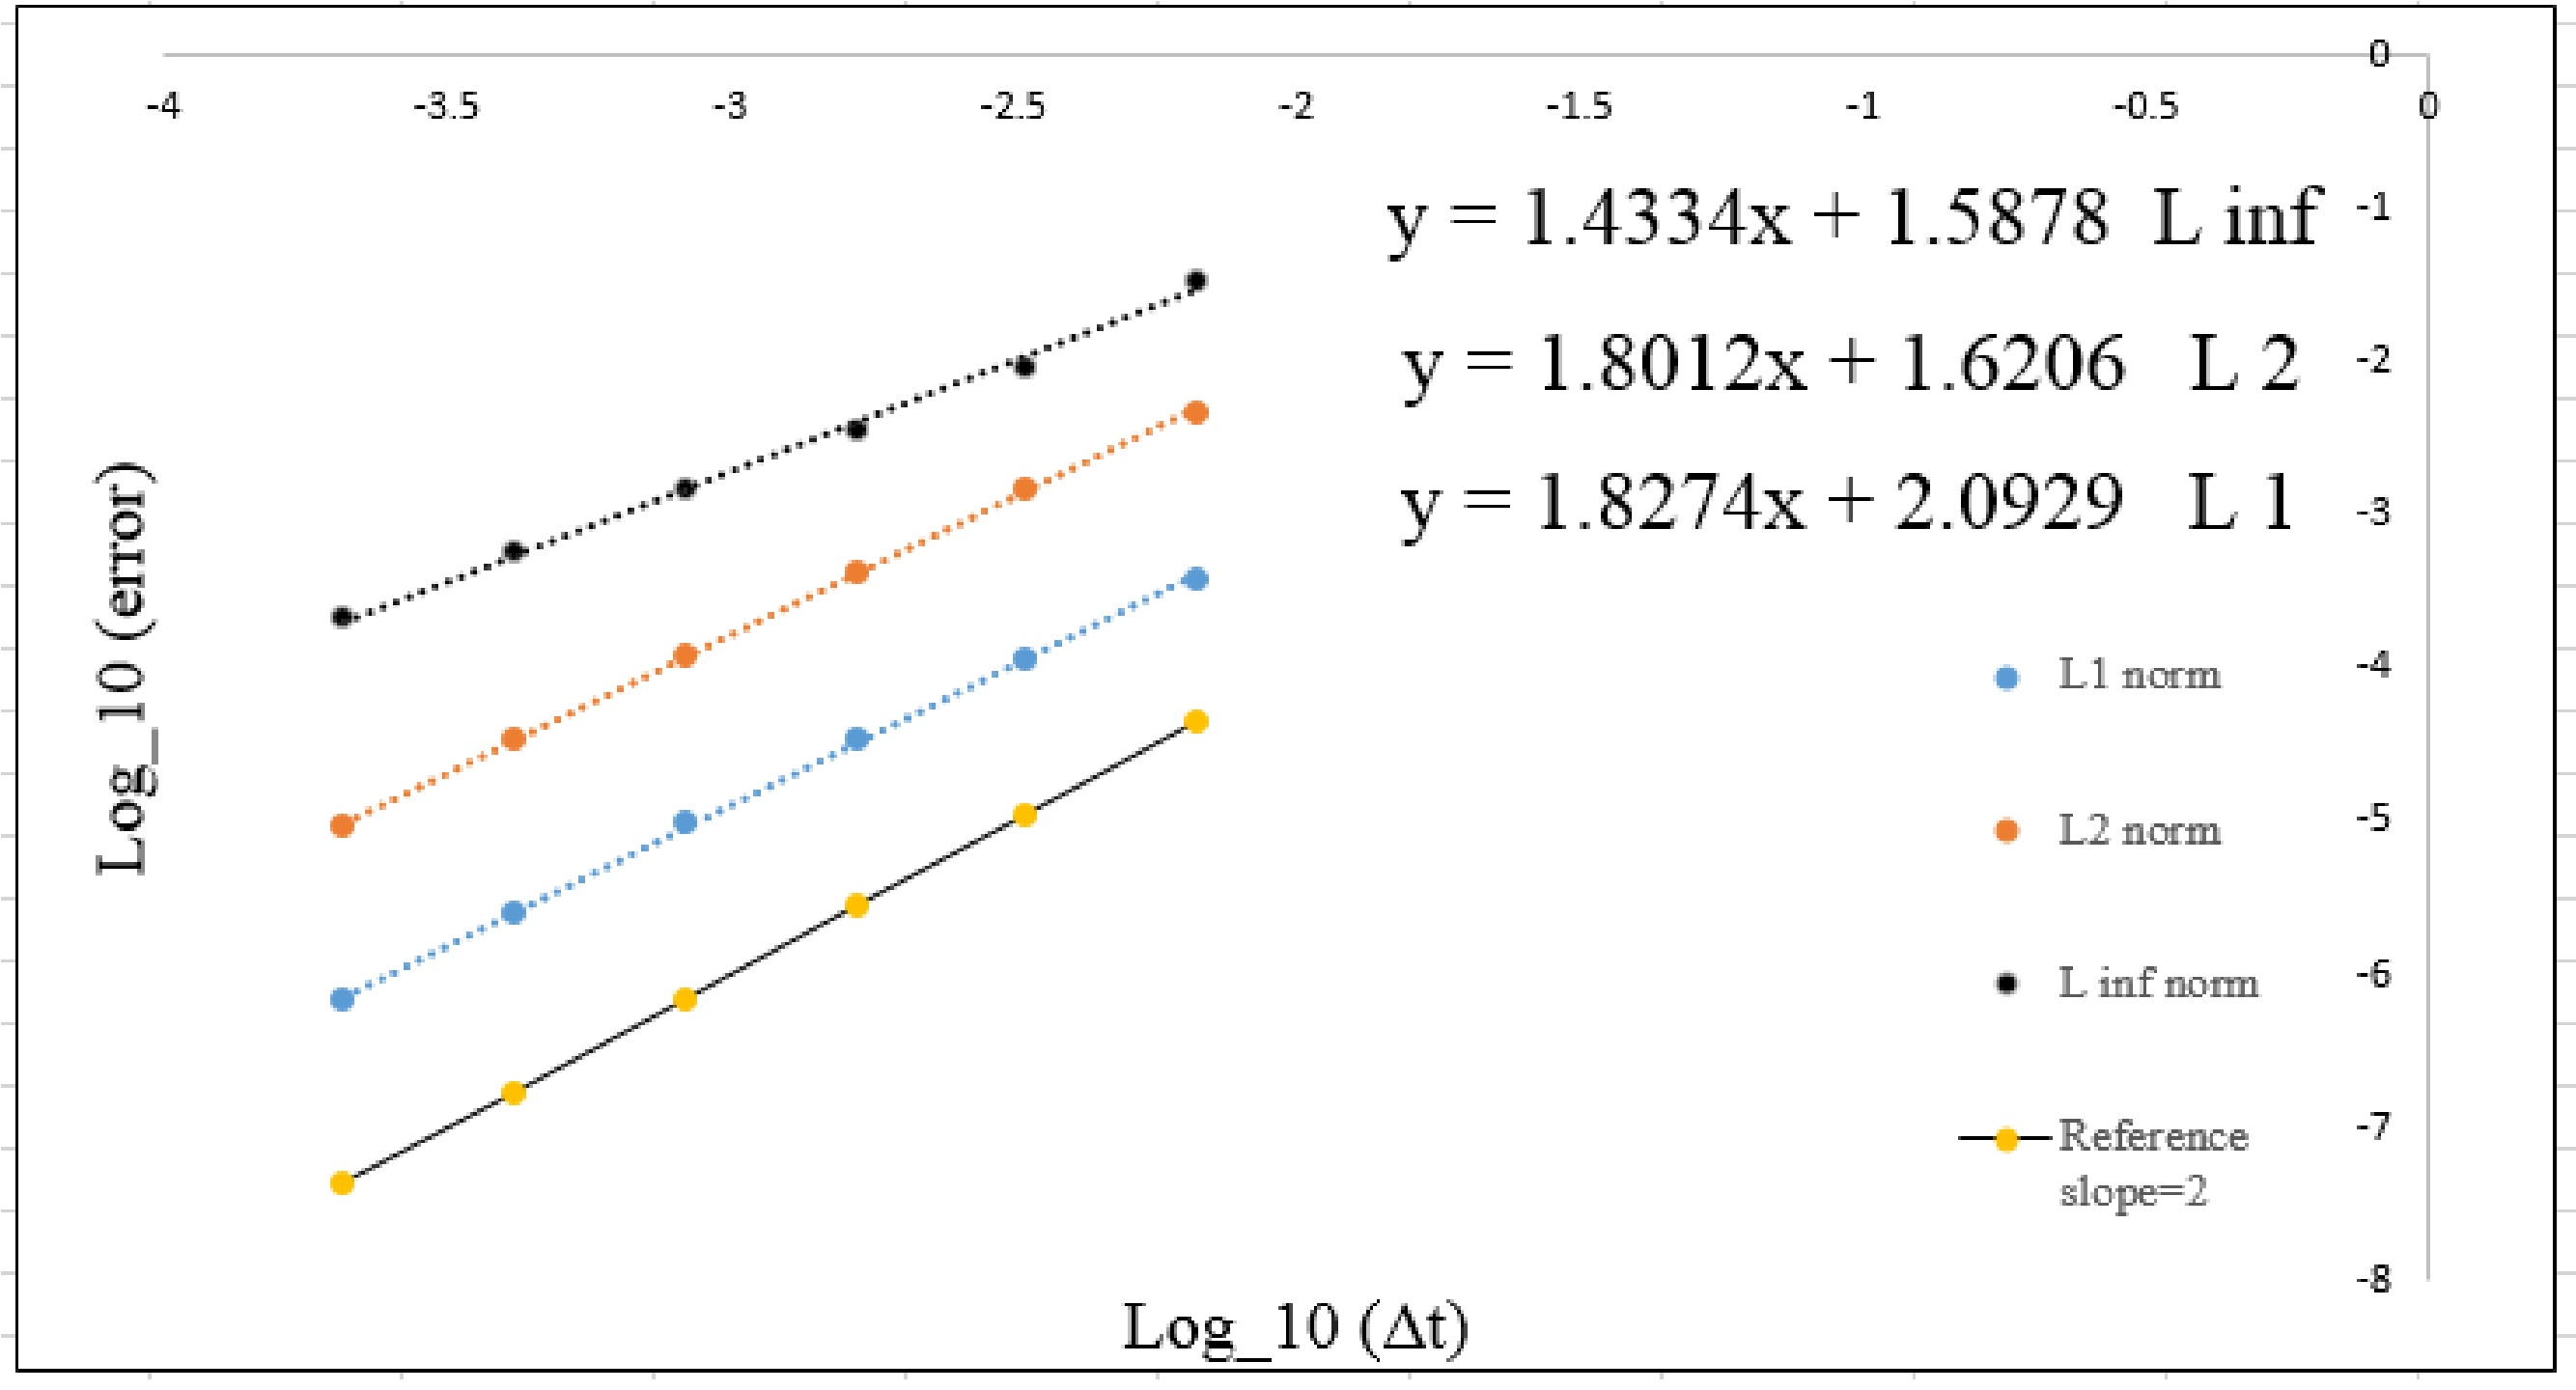
\includegraphics[width=4.5in]{C:/Users/HONGJI/Latex Home directory/Pm1b_pf2_np_div_uv_rate_c_0_5.jpg}}
		\caption{Log-Log plot of Convergence rate for $\nabla \cdot \textbf{u}^*$. }\label{fig:6.19b}
	\end{subfigure}
	\caption{Plot of Convergence rates for Alg 2 with Normalised Pressure approach used. Domain: $[-1,1]^2$, time = 1 and CFL = 0.5. In each plot, the data points corresponding to grid sizes of 15, 30, 60, 120, 240, and 480. Subplot (b) shows the error in the divergence of intermediate velocity. The data points between different norms are close to each. Hence $L_1$ and $L_\infty$ norms were shifted up and down by 0.5 respectively to distinguish from $L_2$ norm data points.}\label{fig:6.16}
\end{figure}

\begin{figure}[H]
	\centering
	\begin{subfigure}[t]{4.5in}
		\centering
		\scalebox{1.2}{
		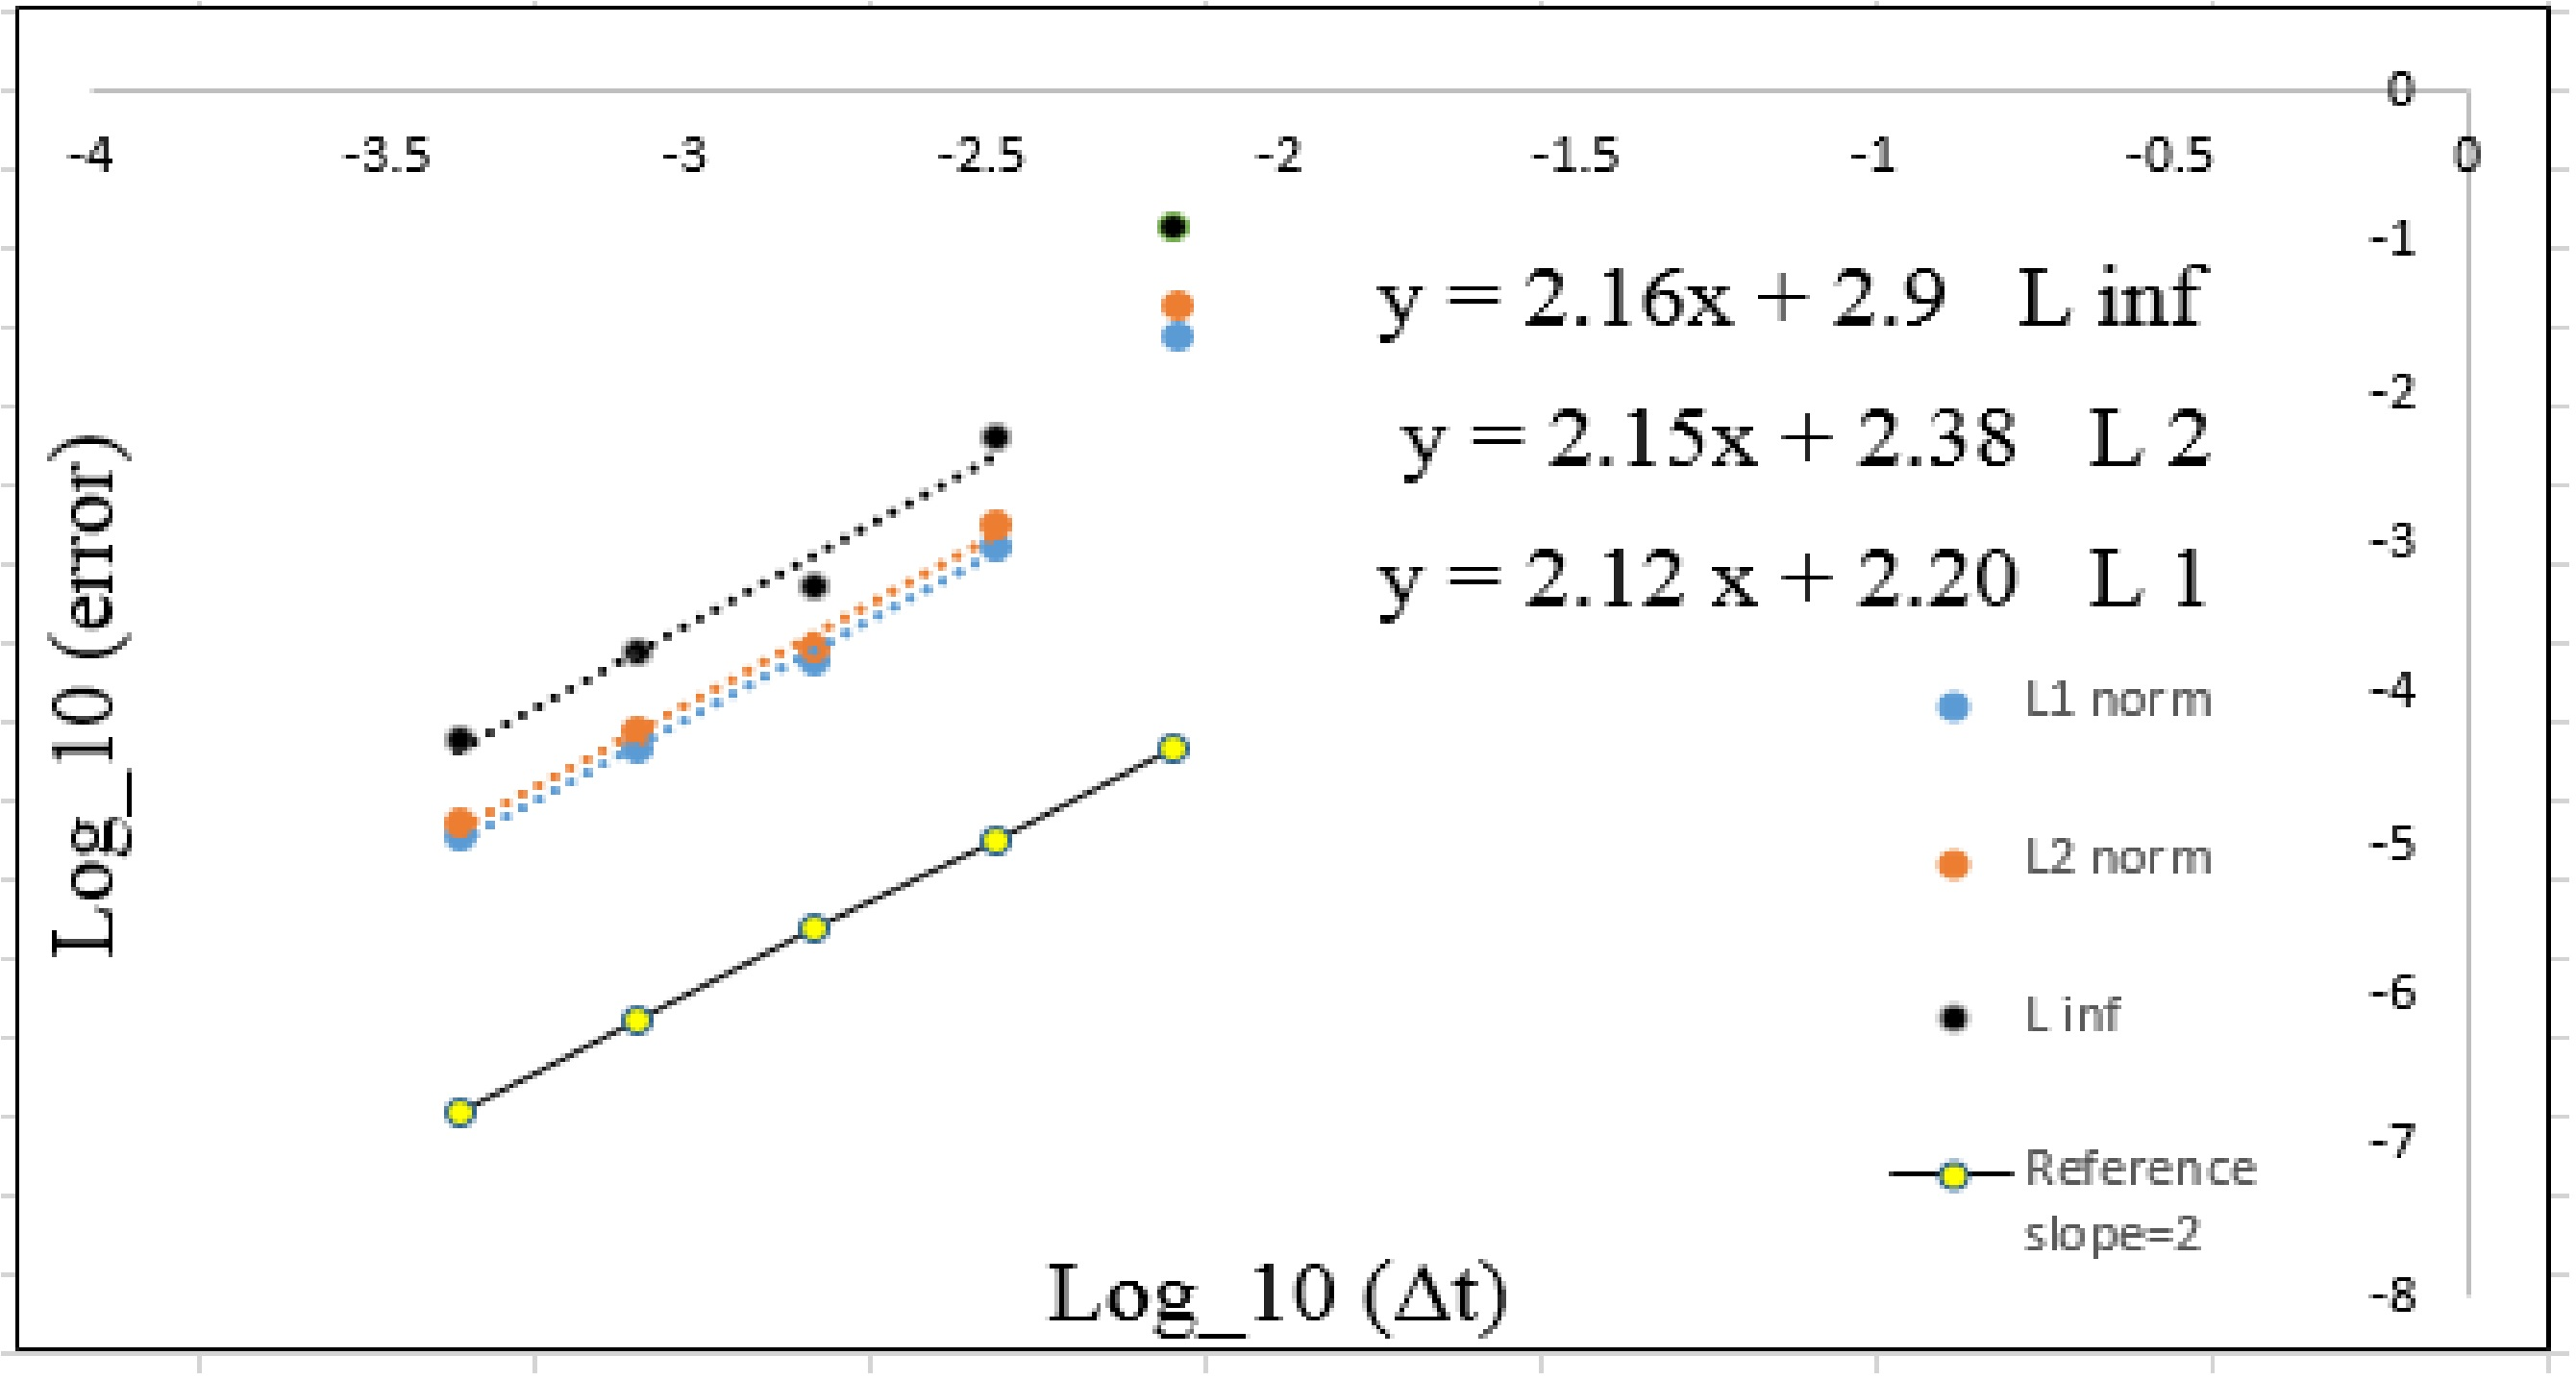
\includegraphics[width=4.5in]{C:/Users/HONGJI/Latex Home directory/Pm2_pf2_np_P_rate_c_0_5.jpg}}
		\caption{Log-Log plot of Convergence rate for Pressure}\label{fig:6.19a}		
	\end{subfigure}
	\quad
	\begin{subfigure}[t]{4.5in}
		\centering
		\scalebox{1.2}{
		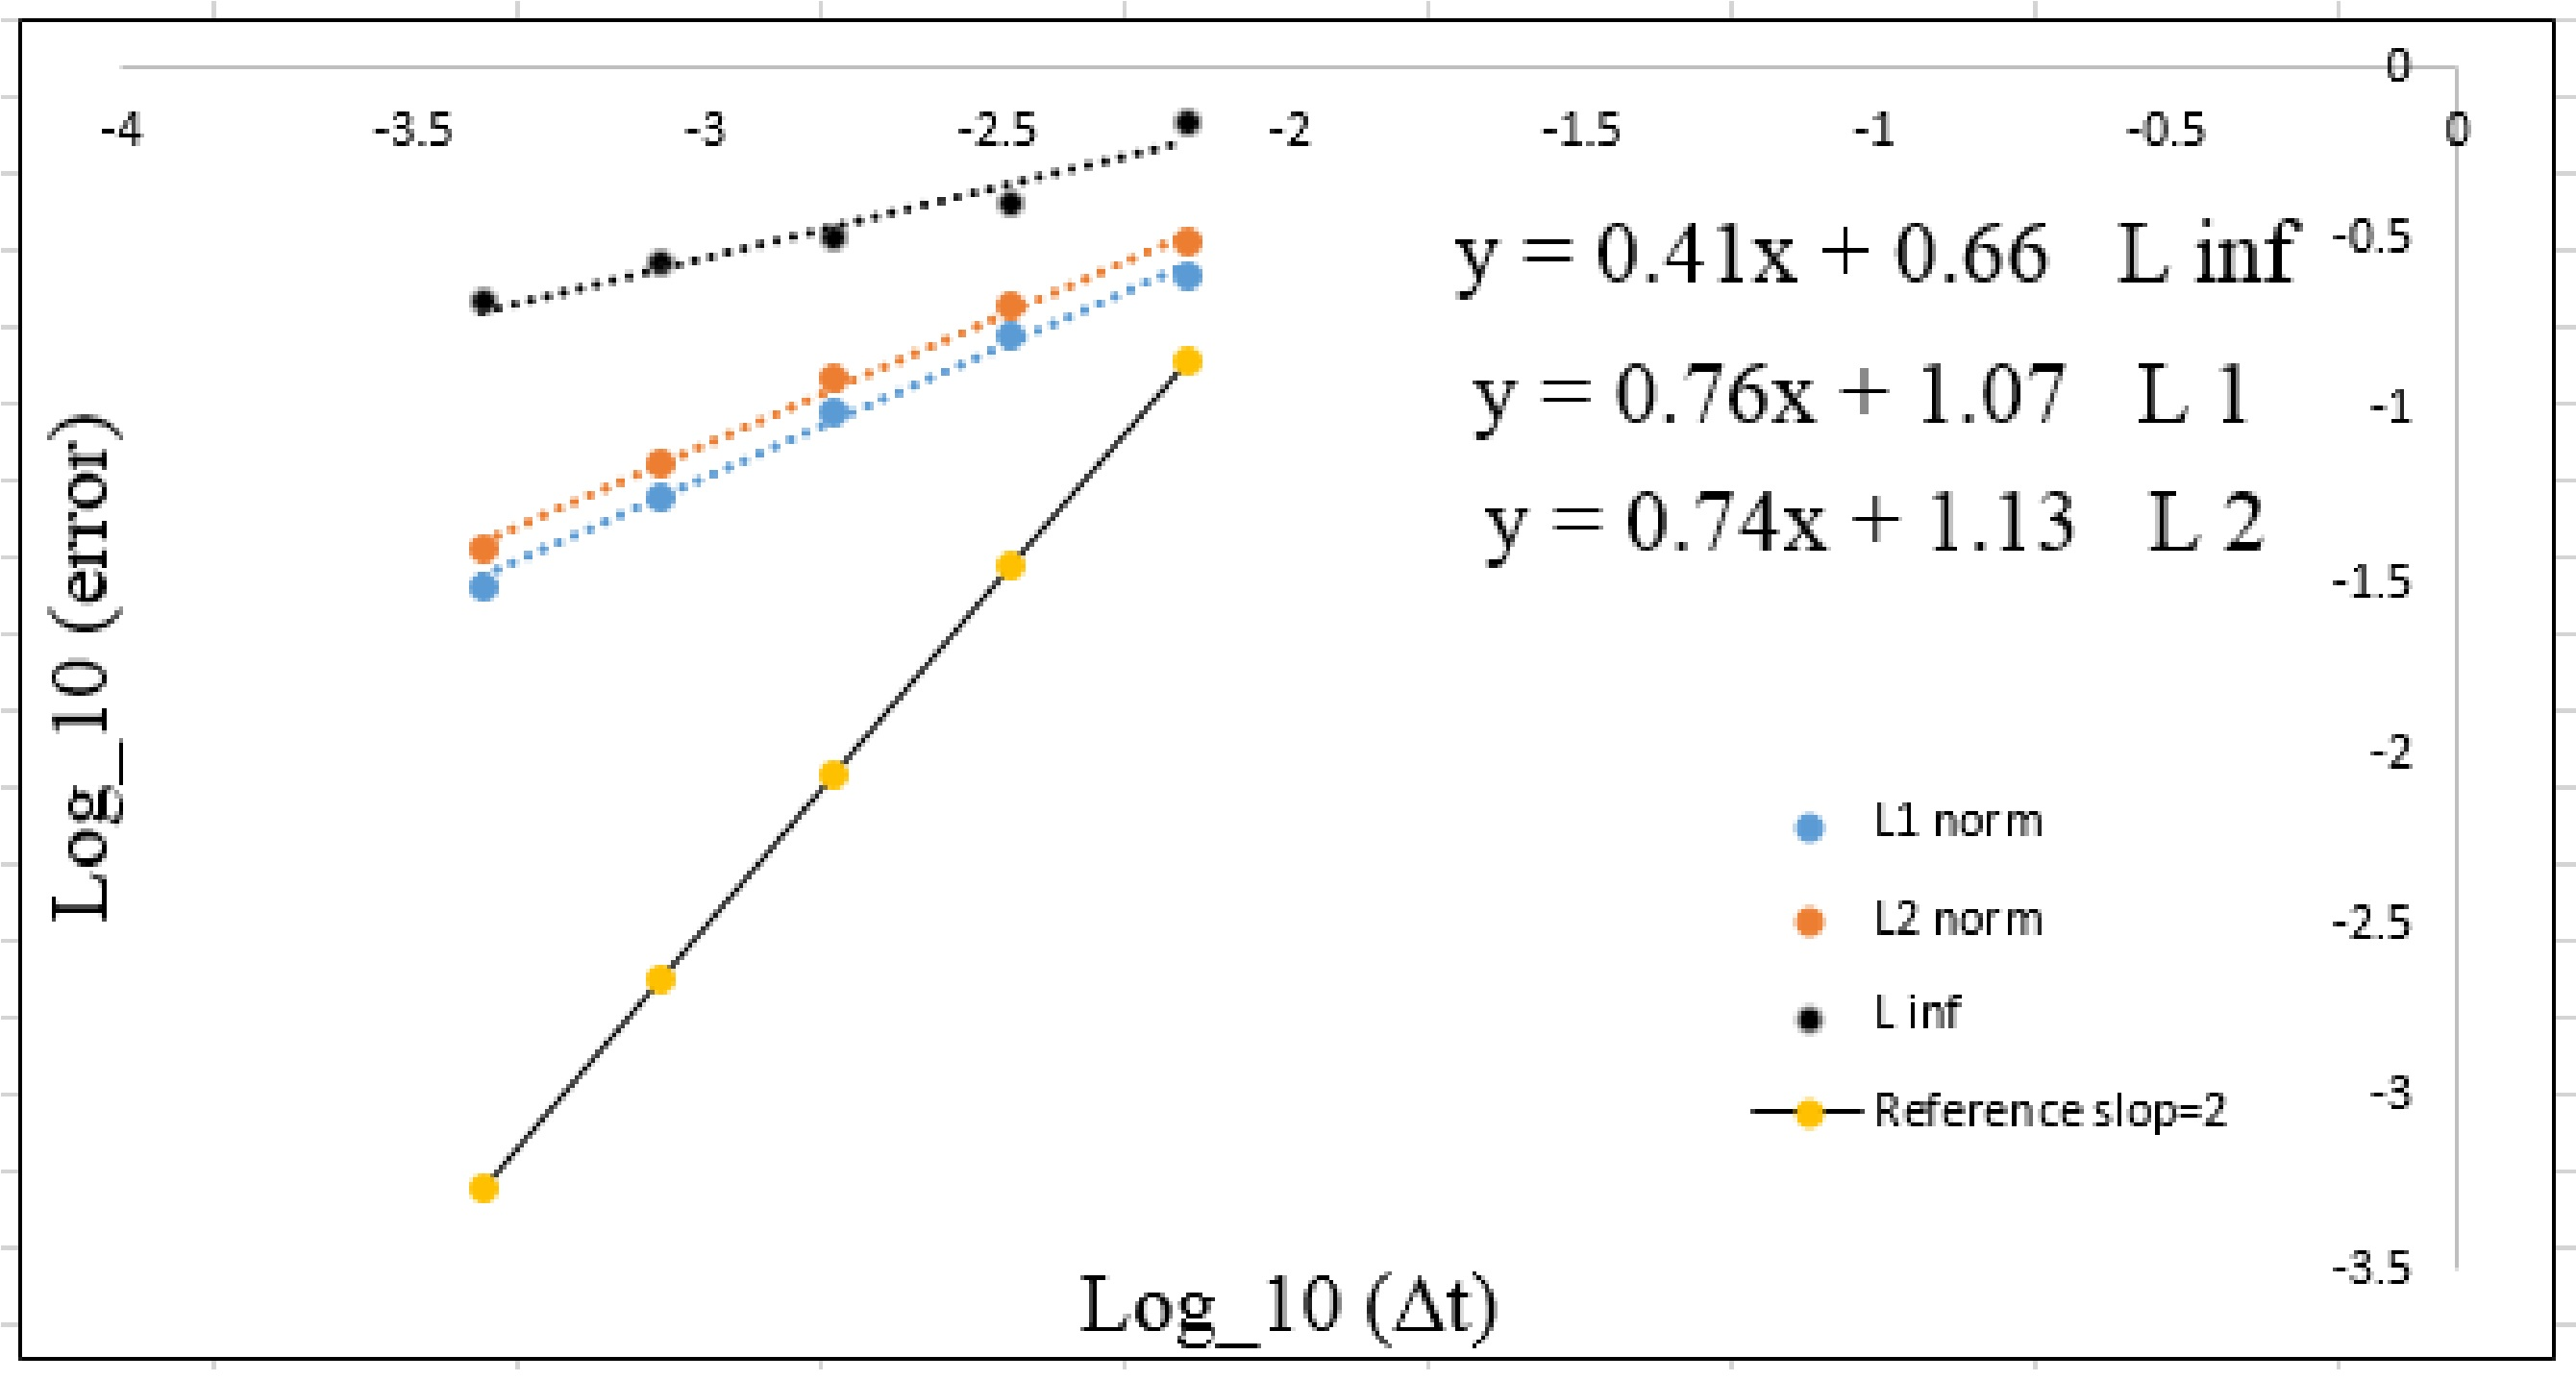
\includegraphics[width=4.5in]{C:/Users/HONGJI/Latex Home directory/Pm2_pf2_np_div_uvstar_rate_c_0_5.jpg}}
		\caption{Log-Log plot of Convergence rate for $\nabla \cdot \textbf{u}^*$. }\label{fig:6.19b}
	\end{subfigure}
	\caption{Plot of Convergence rates for Alg 3 with Normalised Pressure approach used. Domain: $[-1,1]^2$, time = 1 and CFL = 0.5. In each plot, the data points corresponding to grid sizes of 15, 30, 60, 120, 240.}\label{fig:6.16}
\end{figure}

\begin{figure}[H]
	\centering
	\scalebox{1.2}{
	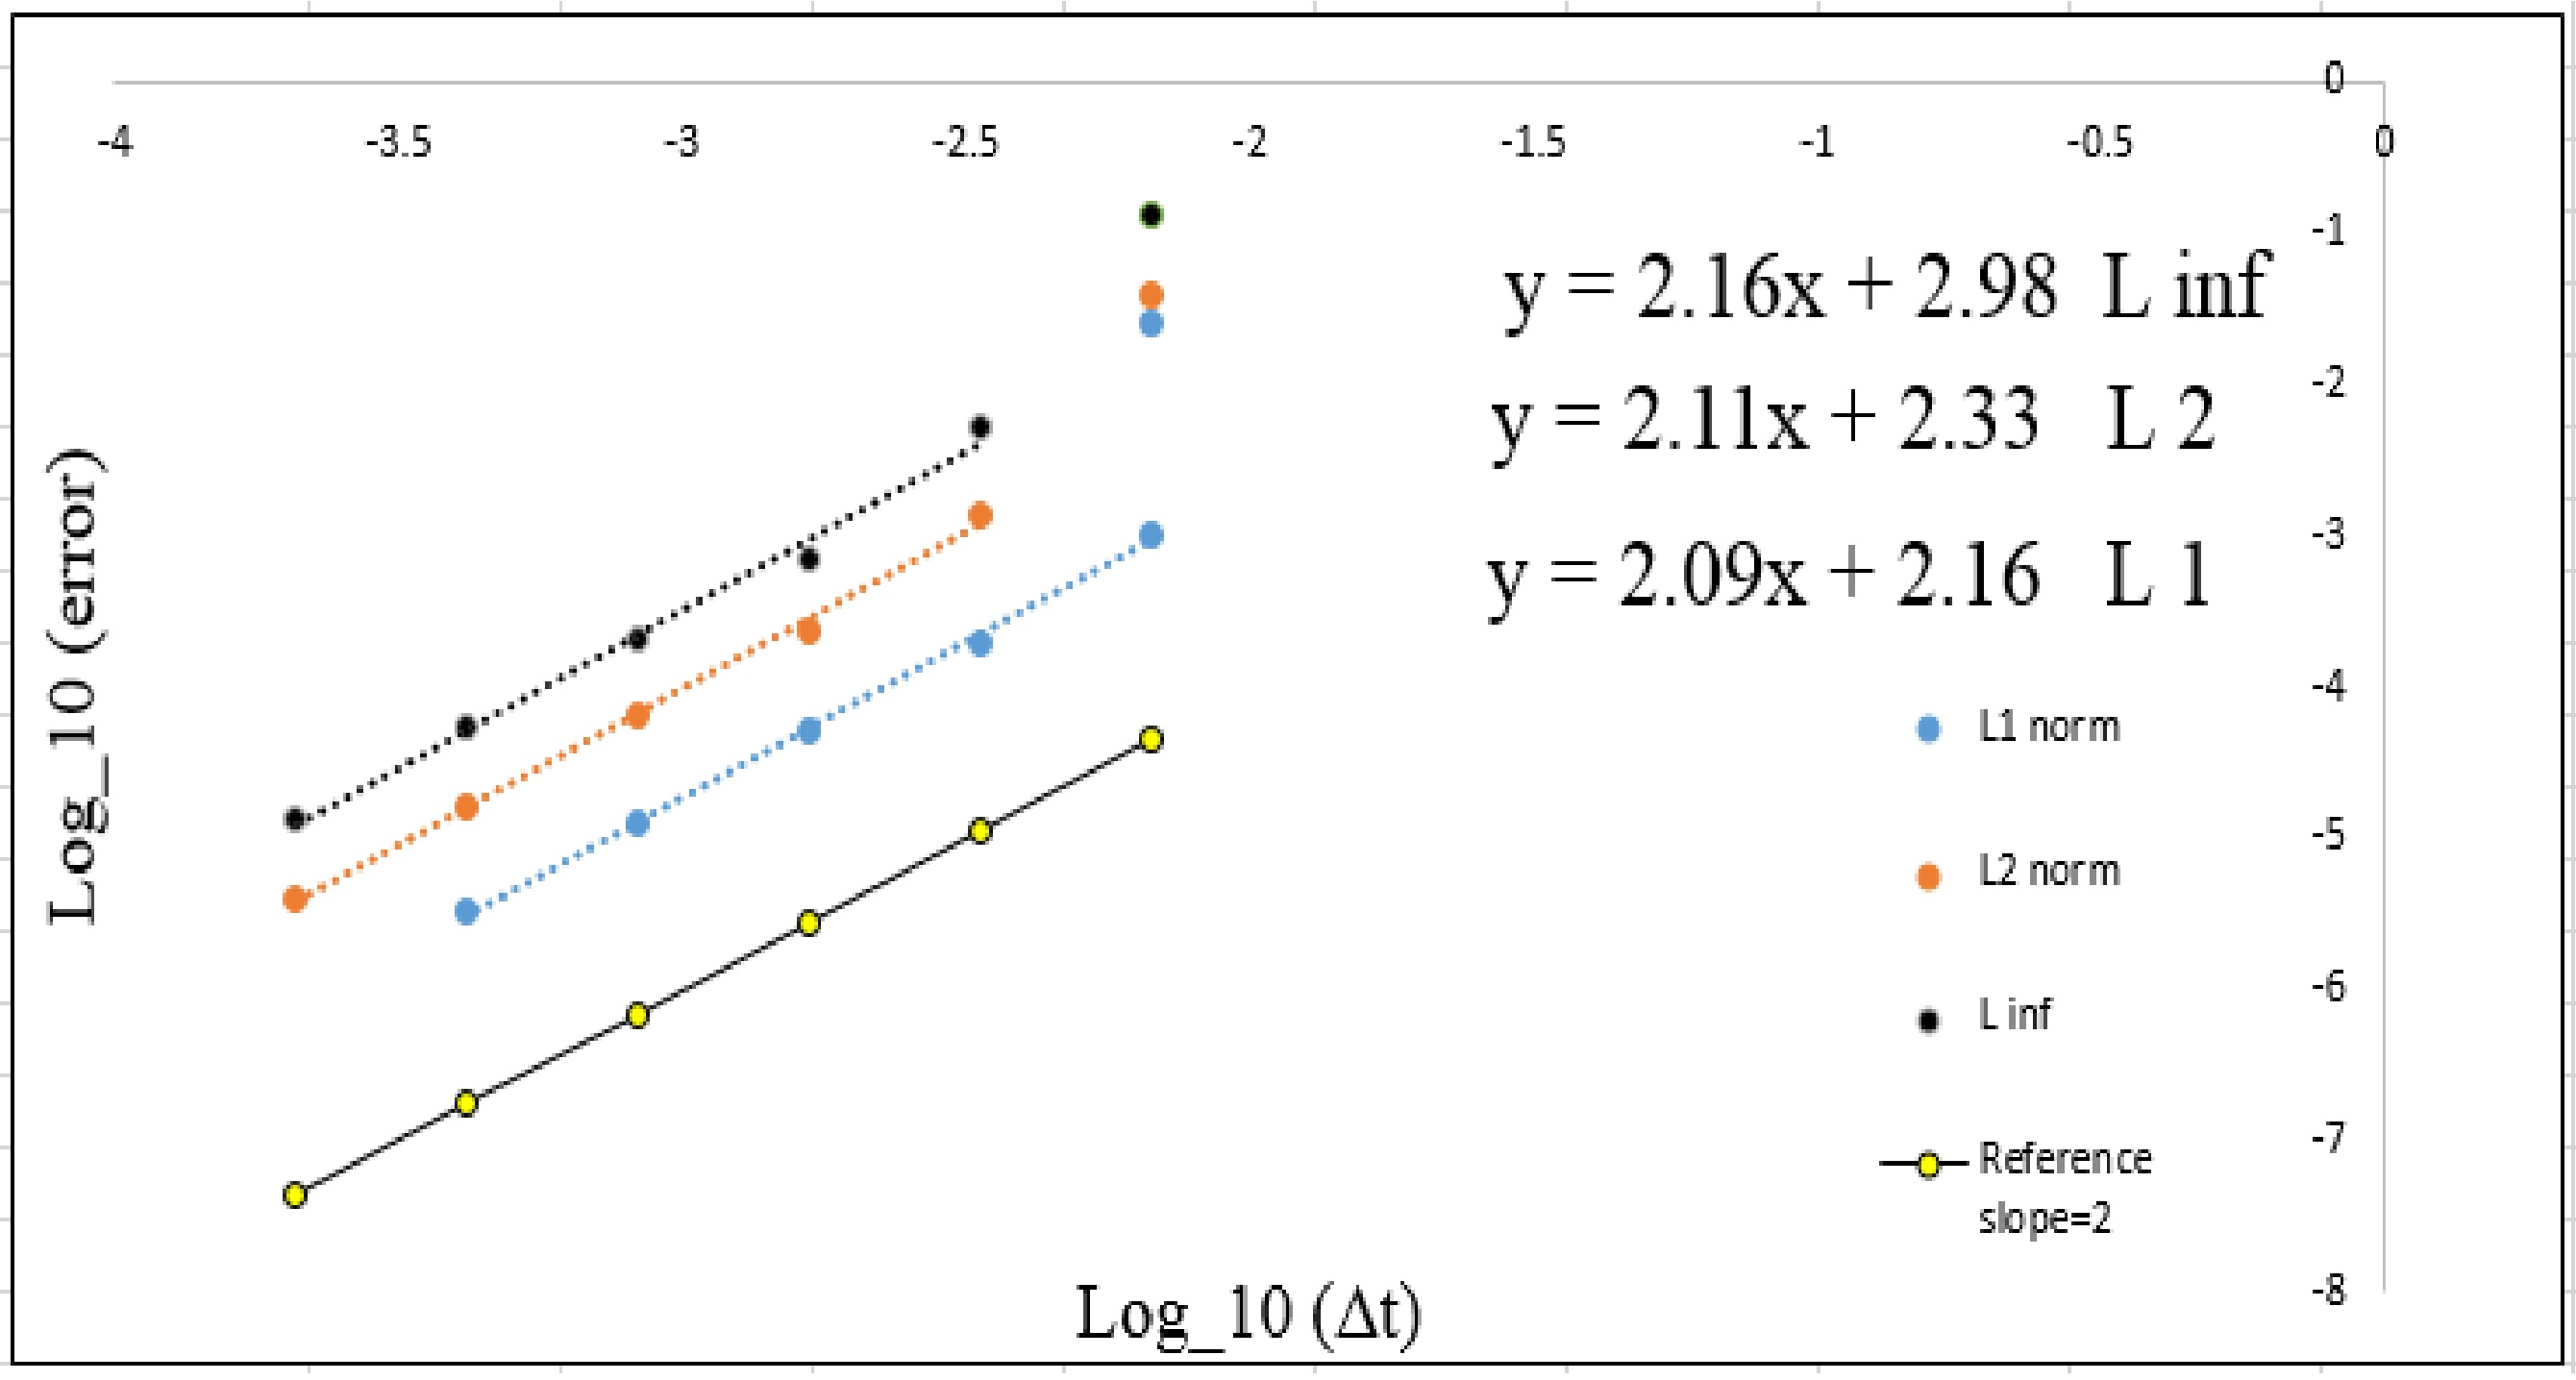
\includegraphics[width=4.5in]{C:/Users/HONGJI/Latex Home directory/Gauge_pf2_np_P_rate_c_0_5.jpg}}
	\caption{Long-Log plot of Pressure Convergence rates for Gauge method with Normalised Pressure approach used. Domain: $[-1,1]^2$, time = 1 and CFL = 0.5. The data points corresponding to grid sizes of 15, 30, 60, 120, 240, and 480.}\label{fig:6.16}
\end{figure}

\begin{figure}[H]
	\centering
	\begin{subfigure}[t]{2.2in}
		\centering
		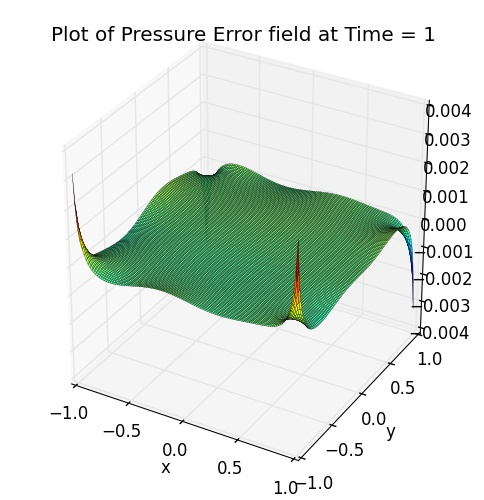
\includegraphics[width=2.2in]{C:/Users/HONGJI/Latex Home directory/Pm1b_pf2_np_P_error_t_1_grid_120.jpg}
		\caption{Pressure error field for Alg 2 method}\label{fig:6.19a}		
	\end{subfigure}
	\quad
	\begin{subfigure}[t]{2.8in}
		\centering
		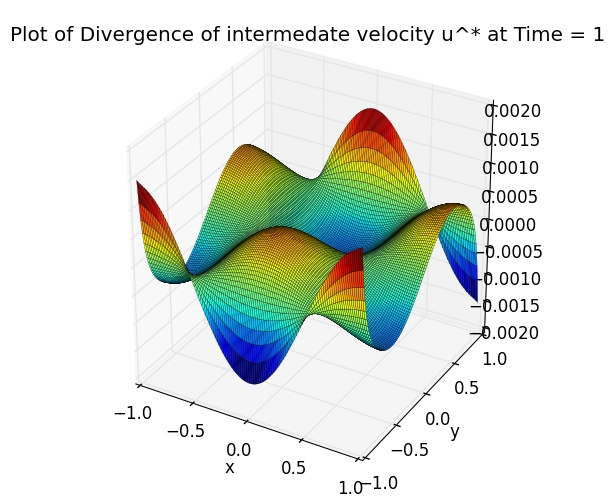
\includegraphics[width=2.8in]{C:/Users/HONGJI/Latex Home directory/Pm1b_pf2_np_div_uvstar_t_1_grid_120.jpg}
		\caption{Divergence of intermediate velocity field for Alg 2 method. }\label{fig:6.19b}
	\end{subfigure}
	\quad
	\centering
	\begin{subfigure}[t]{2.2in}
		\centering
		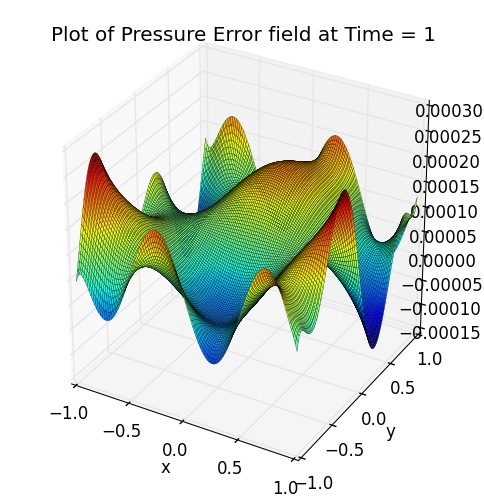
\includegraphics[width=2.2in]{C:/Users/HONGJI/Latex Home directory/Pm2_pf2_cN_np_P_error_t_1_grid_120.jpg}
		\caption{Pressure error field for Alg 3 method}\label{fig:6.19c}		
	\end{subfigure}
	\quad
	\begin{subfigure}[t]{2.6in}
		\centering
		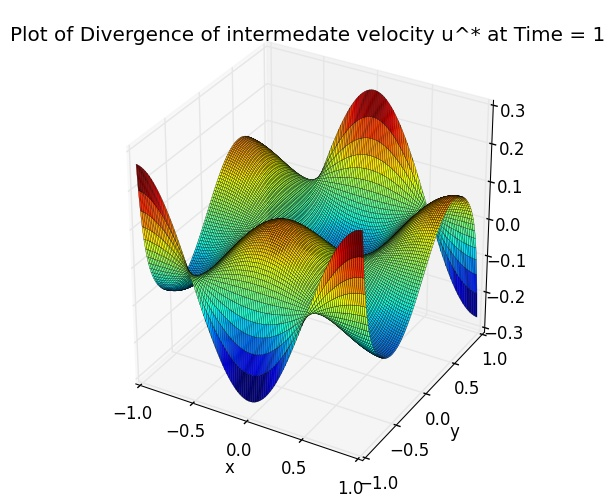
\includegraphics[width=2.6in]{C:/Users/HONGJI/Latex Home directory/Pm2_pf2_cN_np_div_uvstar_t_1_grid_120.jpg}
		\caption{Divergence of intermediate velocity field for Alg 3 method.}\label{fig:6.19d}
	\end{subfigure}
	\quad
	\begin{subfigure}[t]{2.5in}
		\centering
		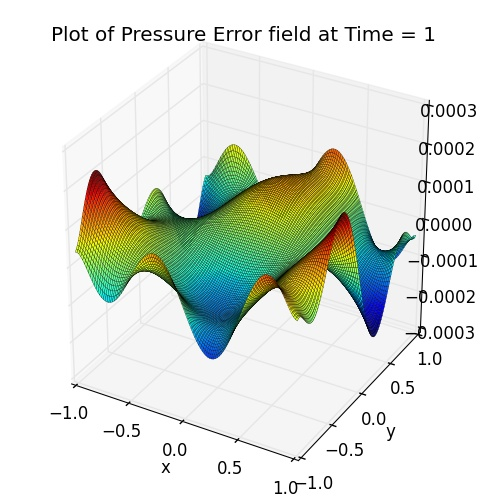
\includegraphics[width=2.5in]{C:/Users/HONGJI/Latex Home directory/Gauge_pf2_P_error_t_1_grid_120.jpg}
		\caption{Pressure error field for Gauge method. }\label{fig:6.19d}
	\end{subfigure}
	\caption{Plots of Pressure error fields and divergence of intermediate velocity for Alg 2, Alg 3 and Gauge method at grid size of 120. Domain: $[-1,1]^2$, time = 1 and CFL = 0.5. }\label{fig:6.16}
\end{figure}

\subsection*{Periodic boundary}
To investigate the performance of projection methods in different boundary conditions, we have implemented a periodic boundary condition in y in order to mimic a periodic channel geometry. The same forced flow problem is considered, but in domain $[-\dfrac{1}{2},\dfrac{1}{2}]^2$. Periodic boundary is ensured by putting the ``ghost cell" values at one side of domain to be equal to the interior points just next to the opposite boundary. For instance, for $U$ velocity at the South boundary ($y = -\dfrac{1}{2}$) we impose the condition: $u_{i-1/2,0} = u_{i-1/2,m}$. This eliminates the spatial interpolation error occurred in calculating the ``ghost cell" values. The exact solutions are once again illustrated below in Figure 6.7. The convergence rates in pressure are also summarised.\\

Interestingly, this time we see all the methods including Alg 2 show second order error convergence in pressure! The $L_\infty$ in Alg 2 is improved to 1.90 (as compared to 1.01 in the previous domain). The pressure error fields and the plot of divergence of intermediate velocity fields for projection methods are also more smooth now. In fact the pressure error fields for Alg 2, Alg 3 and the Gauge method is very similar now, indicating that the periodic geometry recovers second order accuracy for projection methods. This is in agreement with our normal mode analysis done before in Chapter 4 and this also indicate the projection methods (in particular Alg 2) only show optimal pressure error convergence in special domains like the periodic boundary domain whereas the Gauge method shows optimal convergence in general domains too. This finding is in support of Shen et.al results \cite{guermond2004error, guermond2006overview} where they have also given an error bound of 1.5 for projection method (Alg 2 in particular). This shows a limitation in normal mode analysis too. The exact cause of this problem however still remains open in literature.\\

\begin{figure}[H]
	\centering
	\begin{subfigure}[t]{2.5in}
		\centering
		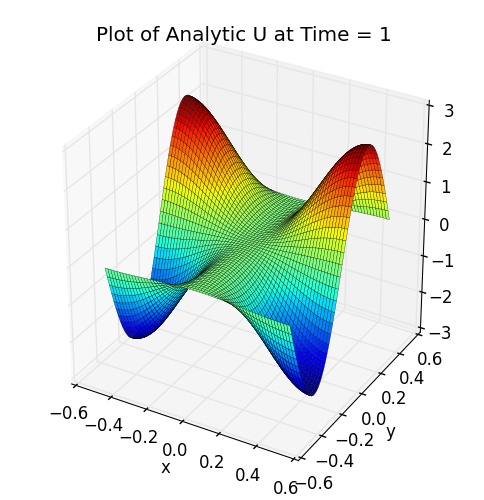
\includegraphics[width=2.5in]{C:/Users/HONGJI/Latex Home directory/Pm1b_pf2b_U_exact_t_1_grid_60.jpg}
		\caption{Analytic $U$ velocity at $t=1$}\label{fig:7.1a}		
	\end{subfigure}
	\quad
	\begin{subfigure}[t]{2.5in}
		\centering
		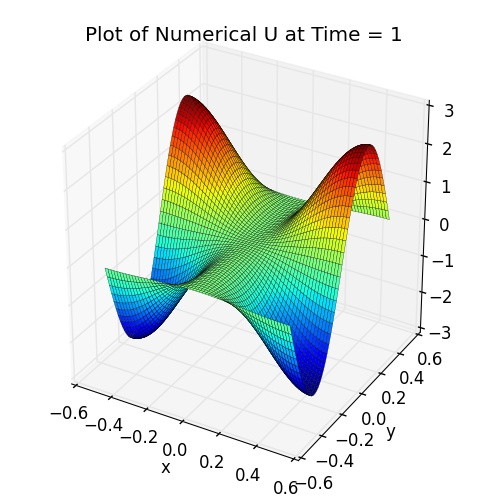
\includegraphics[width=2.5in]{C:/Users/HONGJI/Latex Home directory/Pm1b_pf2b_uf_t_1_grid_60.jpg}
		\caption{Numerical $U$ velocity at $t=1$}\label{fig:7.1b}
	\end{subfigure}
	\quad
	\begin{subfigure}[t]{2.5in}
		\centering
		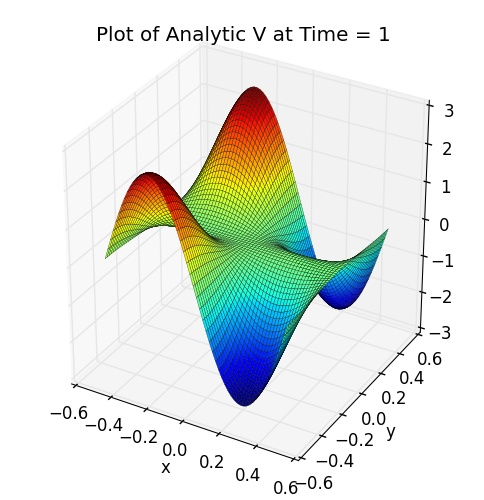
\includegraphics[width=2.5in]{C:/Users/HONGJI/Latex Home directory/Pm1b_pf2b_V_exact_t_1_grid_60.jpg}
		\caption{Analytic $V$ velocity at $t=1$}\label{fig:7.1c}
	\end{subfigure}
	\quad
	\begin{subfigure}[t]{2.5in}
		\centering
		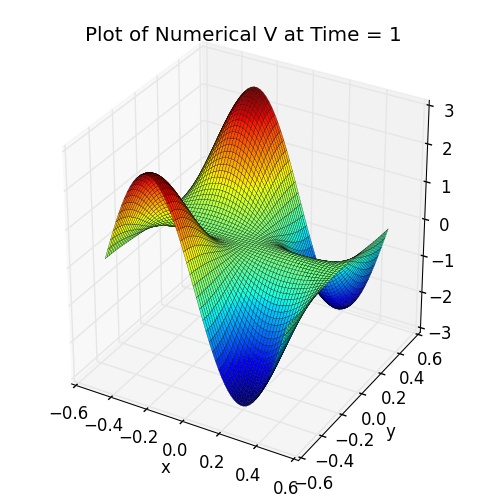
\includegraphics[width=2.5in]{C:/Users/HONGJI/Latex Home directory/Pm1b_pf2b_vf_t_1_grid_60.jpg}
		\caption{Numerical $V$ velocity at $t=1$}\label{fig:7.1d}
	\end{subfigure}
	\quad	
	\begin{subfigure}[t]{2.5in}
		\centering
		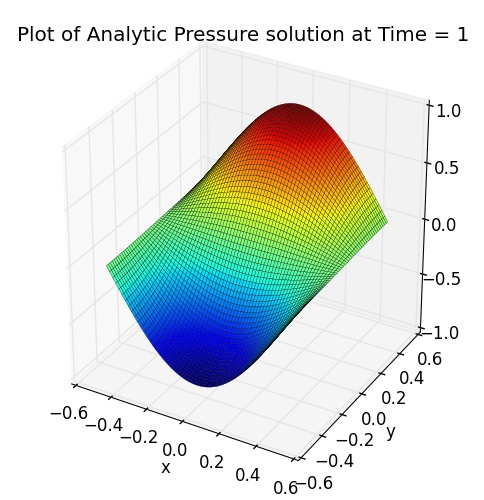
\includegraphics[width=2.5in]{C:/Users/HONGJI/Latex Home directory/Pm1b_pf2b_P_exact_t_1_grid_60.jpg}
		\caption{Analytic pressure ($P$) at $t=1$}\label{fig:7.1e}
	\end{subfigure}
	\quad	
	\begin{subfigure}[t]{2.5in}
		\centering
		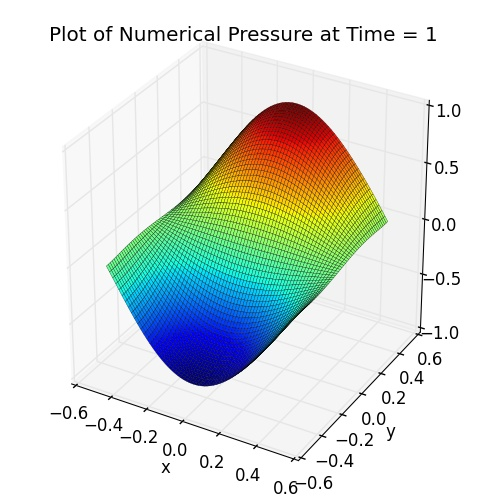
\includegraphics[width=2.5in]{C:/Users/HONGJI/Latex Home directory/Pm1b_pf2b_pf_t_1_grid_60.jpg}
		\caption{Numerical pressure ($P$) at $t=1$}\label{fig:7.1f}
	\end{subfigure}
	\caption{Plot of exact and numerical solutions ($U,V,P$) at time $t=1$ on the spatial domain of $[-\dfrac{1}{2},\dfrac{1}{2}]^2$ with grid size $60 \times 60$. Alg 2 method is used to compute the numerical solutions with $CFL=0.5$}\label{fig:7.1}
\end{figure}

\begin{figure}[H]
	\centering
	\begin{subfigure}[t]{4.5in}
		\centering
		\scalebox{1.2}{
		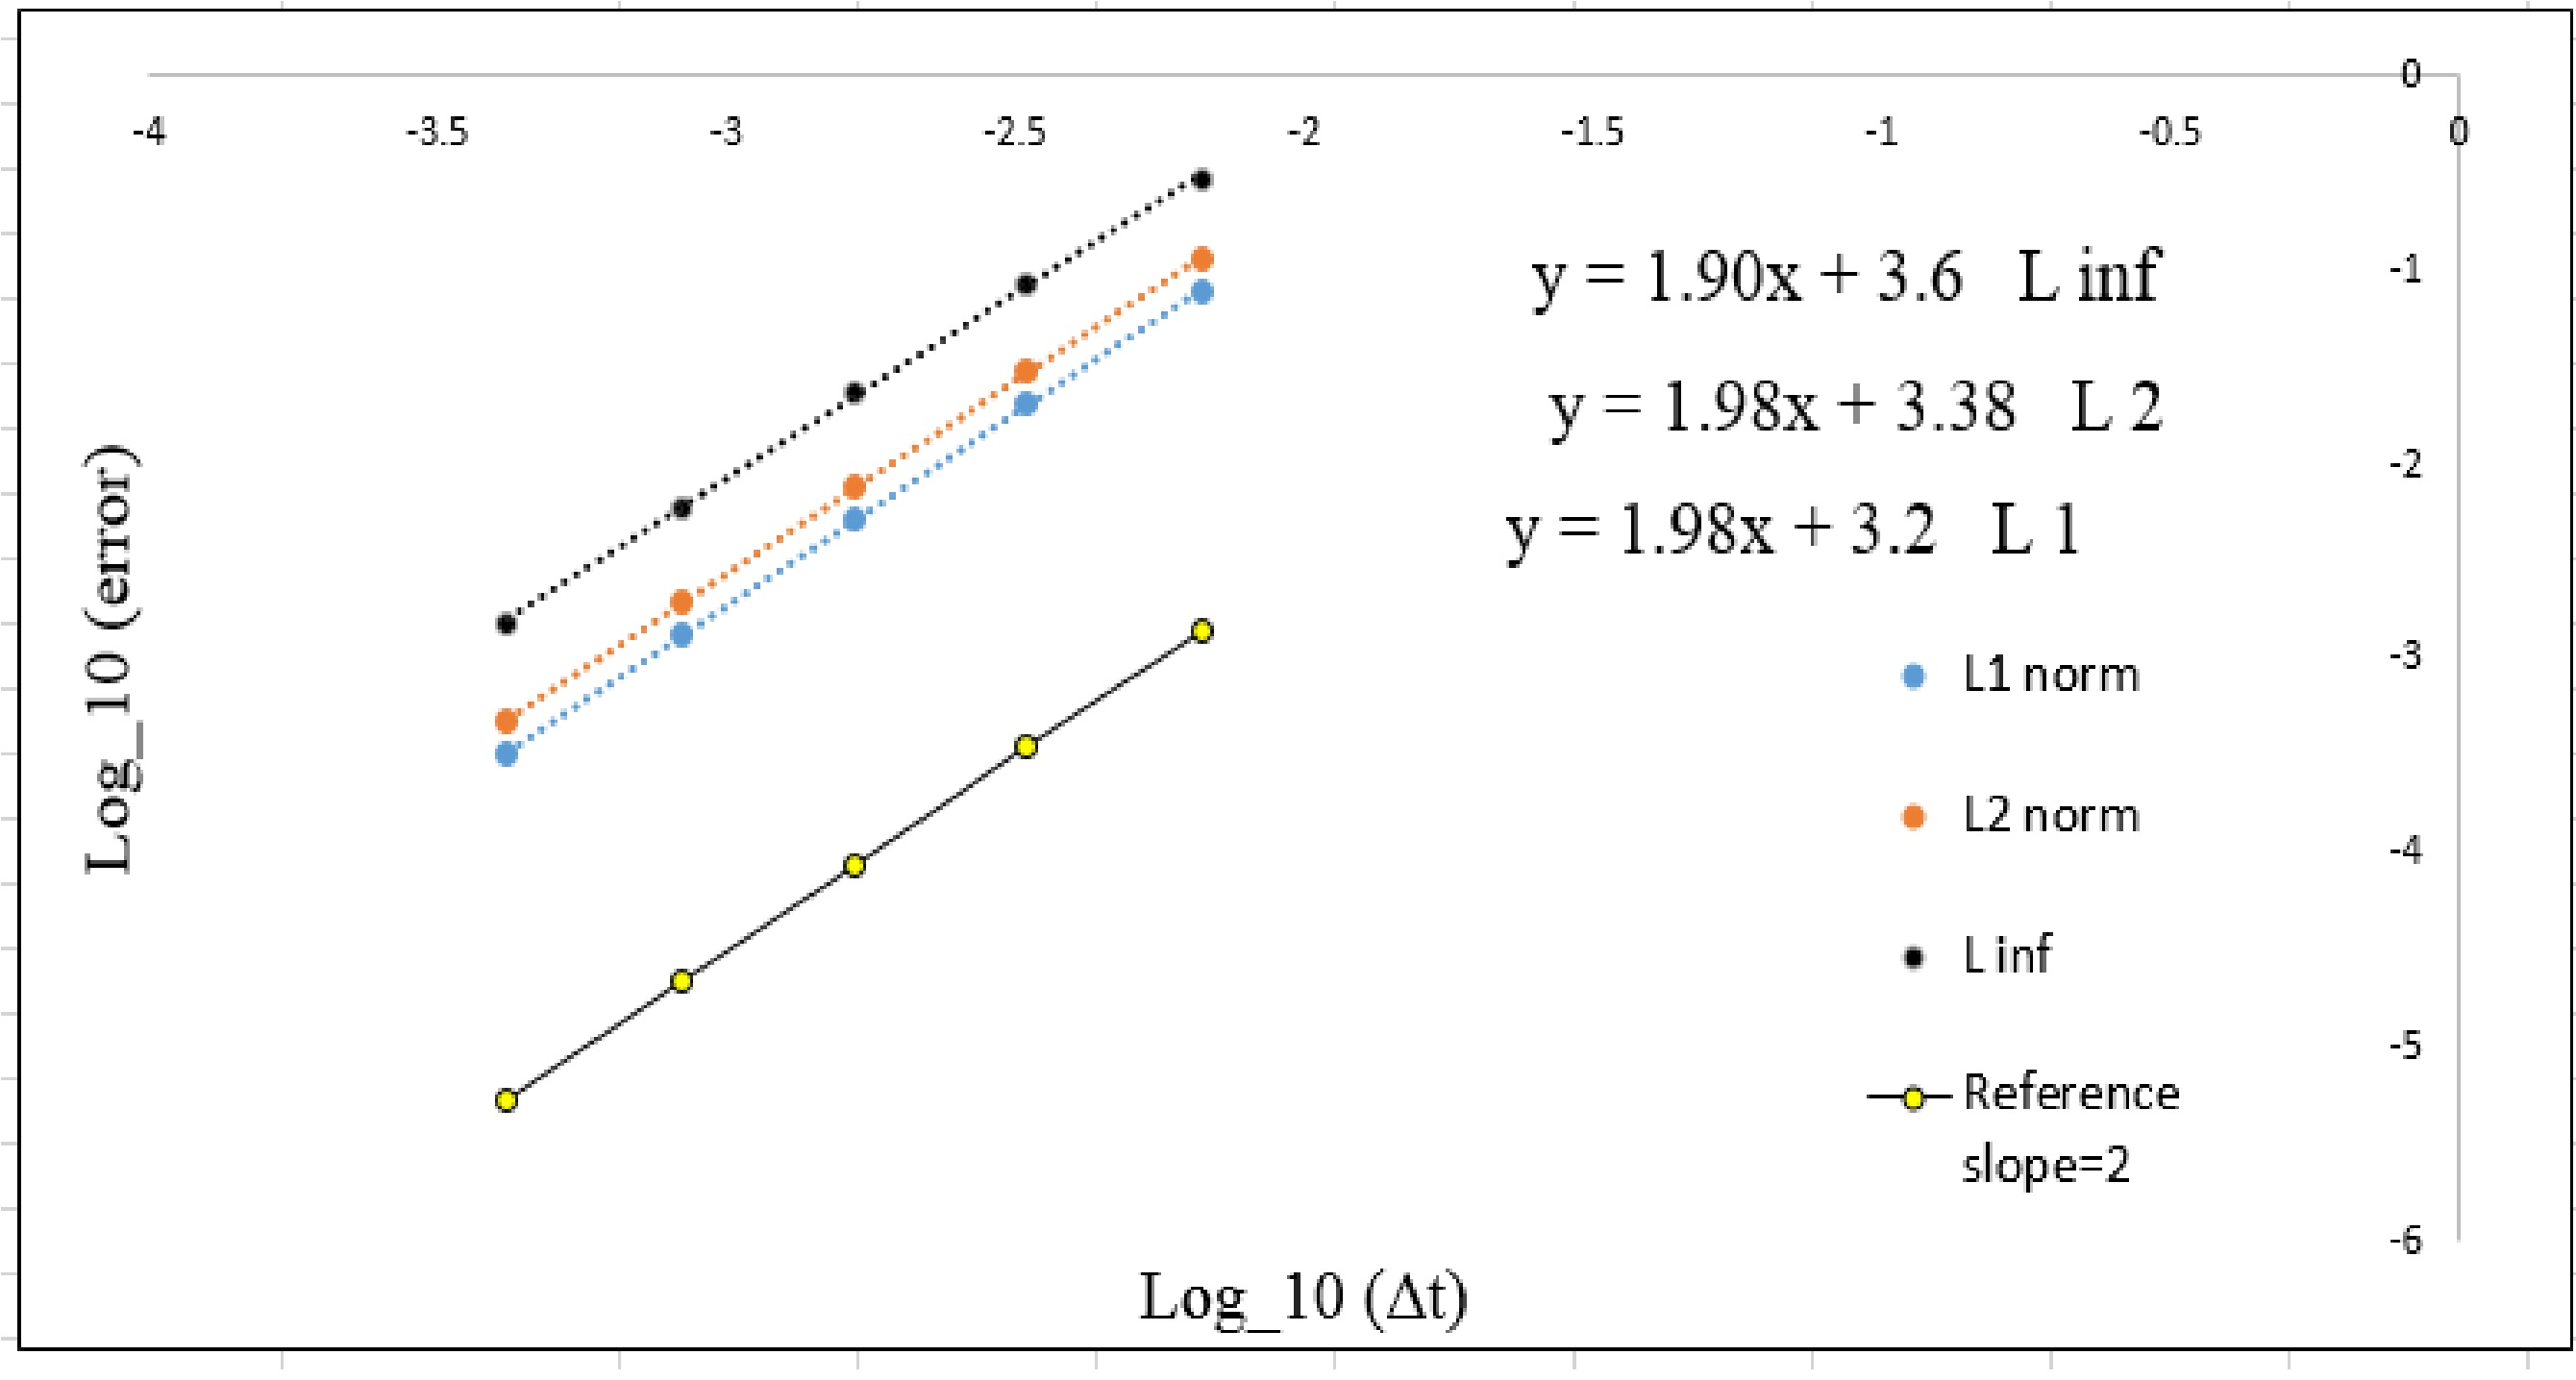
\includegraphics[width=4.5in]{C:/Users/HONGJI/Latex Home directory/Pm1b_pf2b_np_P_rate_c_0_5.jpg}}
		\caption{Log-Log plot of Convergence rate for Pressure}\label{fig:6.19a}		
	\end{subfigure}
	\quad
	\begin{subfigure}[t]{4.5in}
		\centering
		\scalebox{1.2}{
		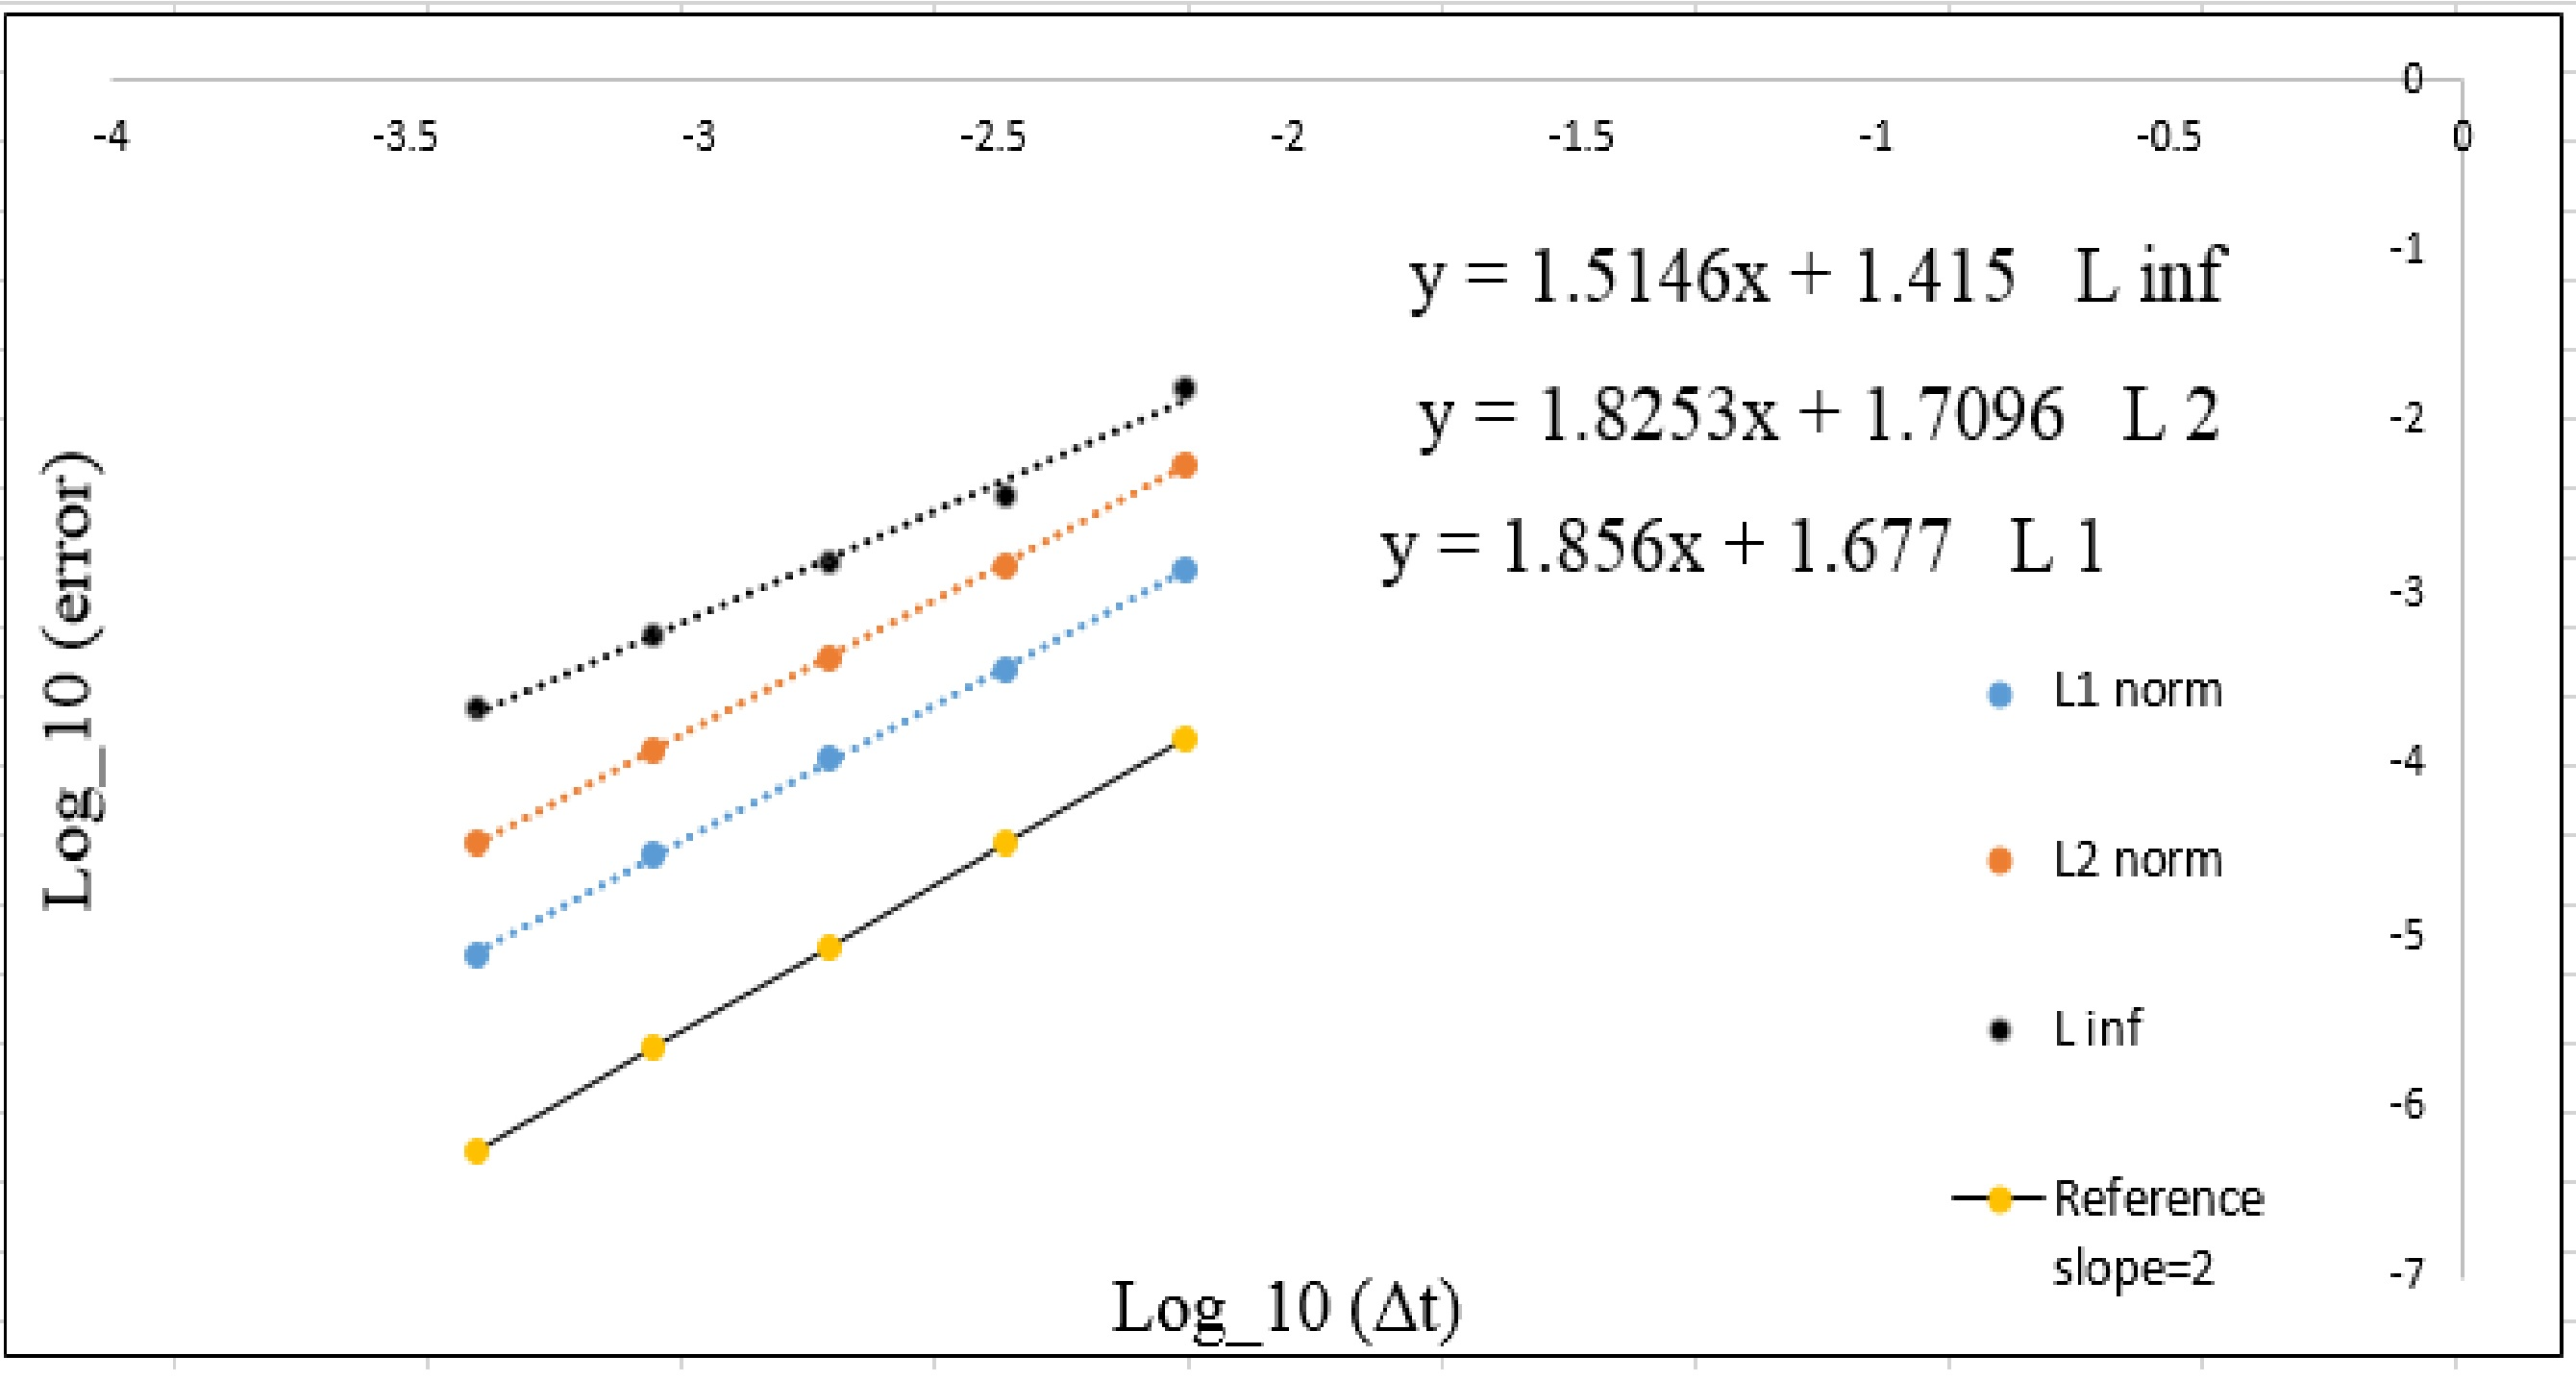
\includegraphics[width=4.5in]{C:/Users/HONGJI/Latex Home directory/Pm1b_pf2b_np_div_uvstar_rate_c_0_5.jpg}}
		\caption{Log-Log plot of Convergence rate for $\nabla \cdot \textbf{u}^*$. }\label{fig:6.19b}
	\end{subfigure}
	\caption{Plot of Convergence rates for Alg 2. Domain:  $[-\dfrac{1}{2}, \dfrac{1}{2}]^2$, time = 1 and CFL = 0.5. In each plot, the data points corresponding to grid sizes of 15, 30, 60, 120, 240.}\label{fig:6.16}
\end{figure}

\begin{figure}[H]
	\centering
	\begin{subfigure}[t]{4.5in}
		\centering
		\scalebox{1.2}{
		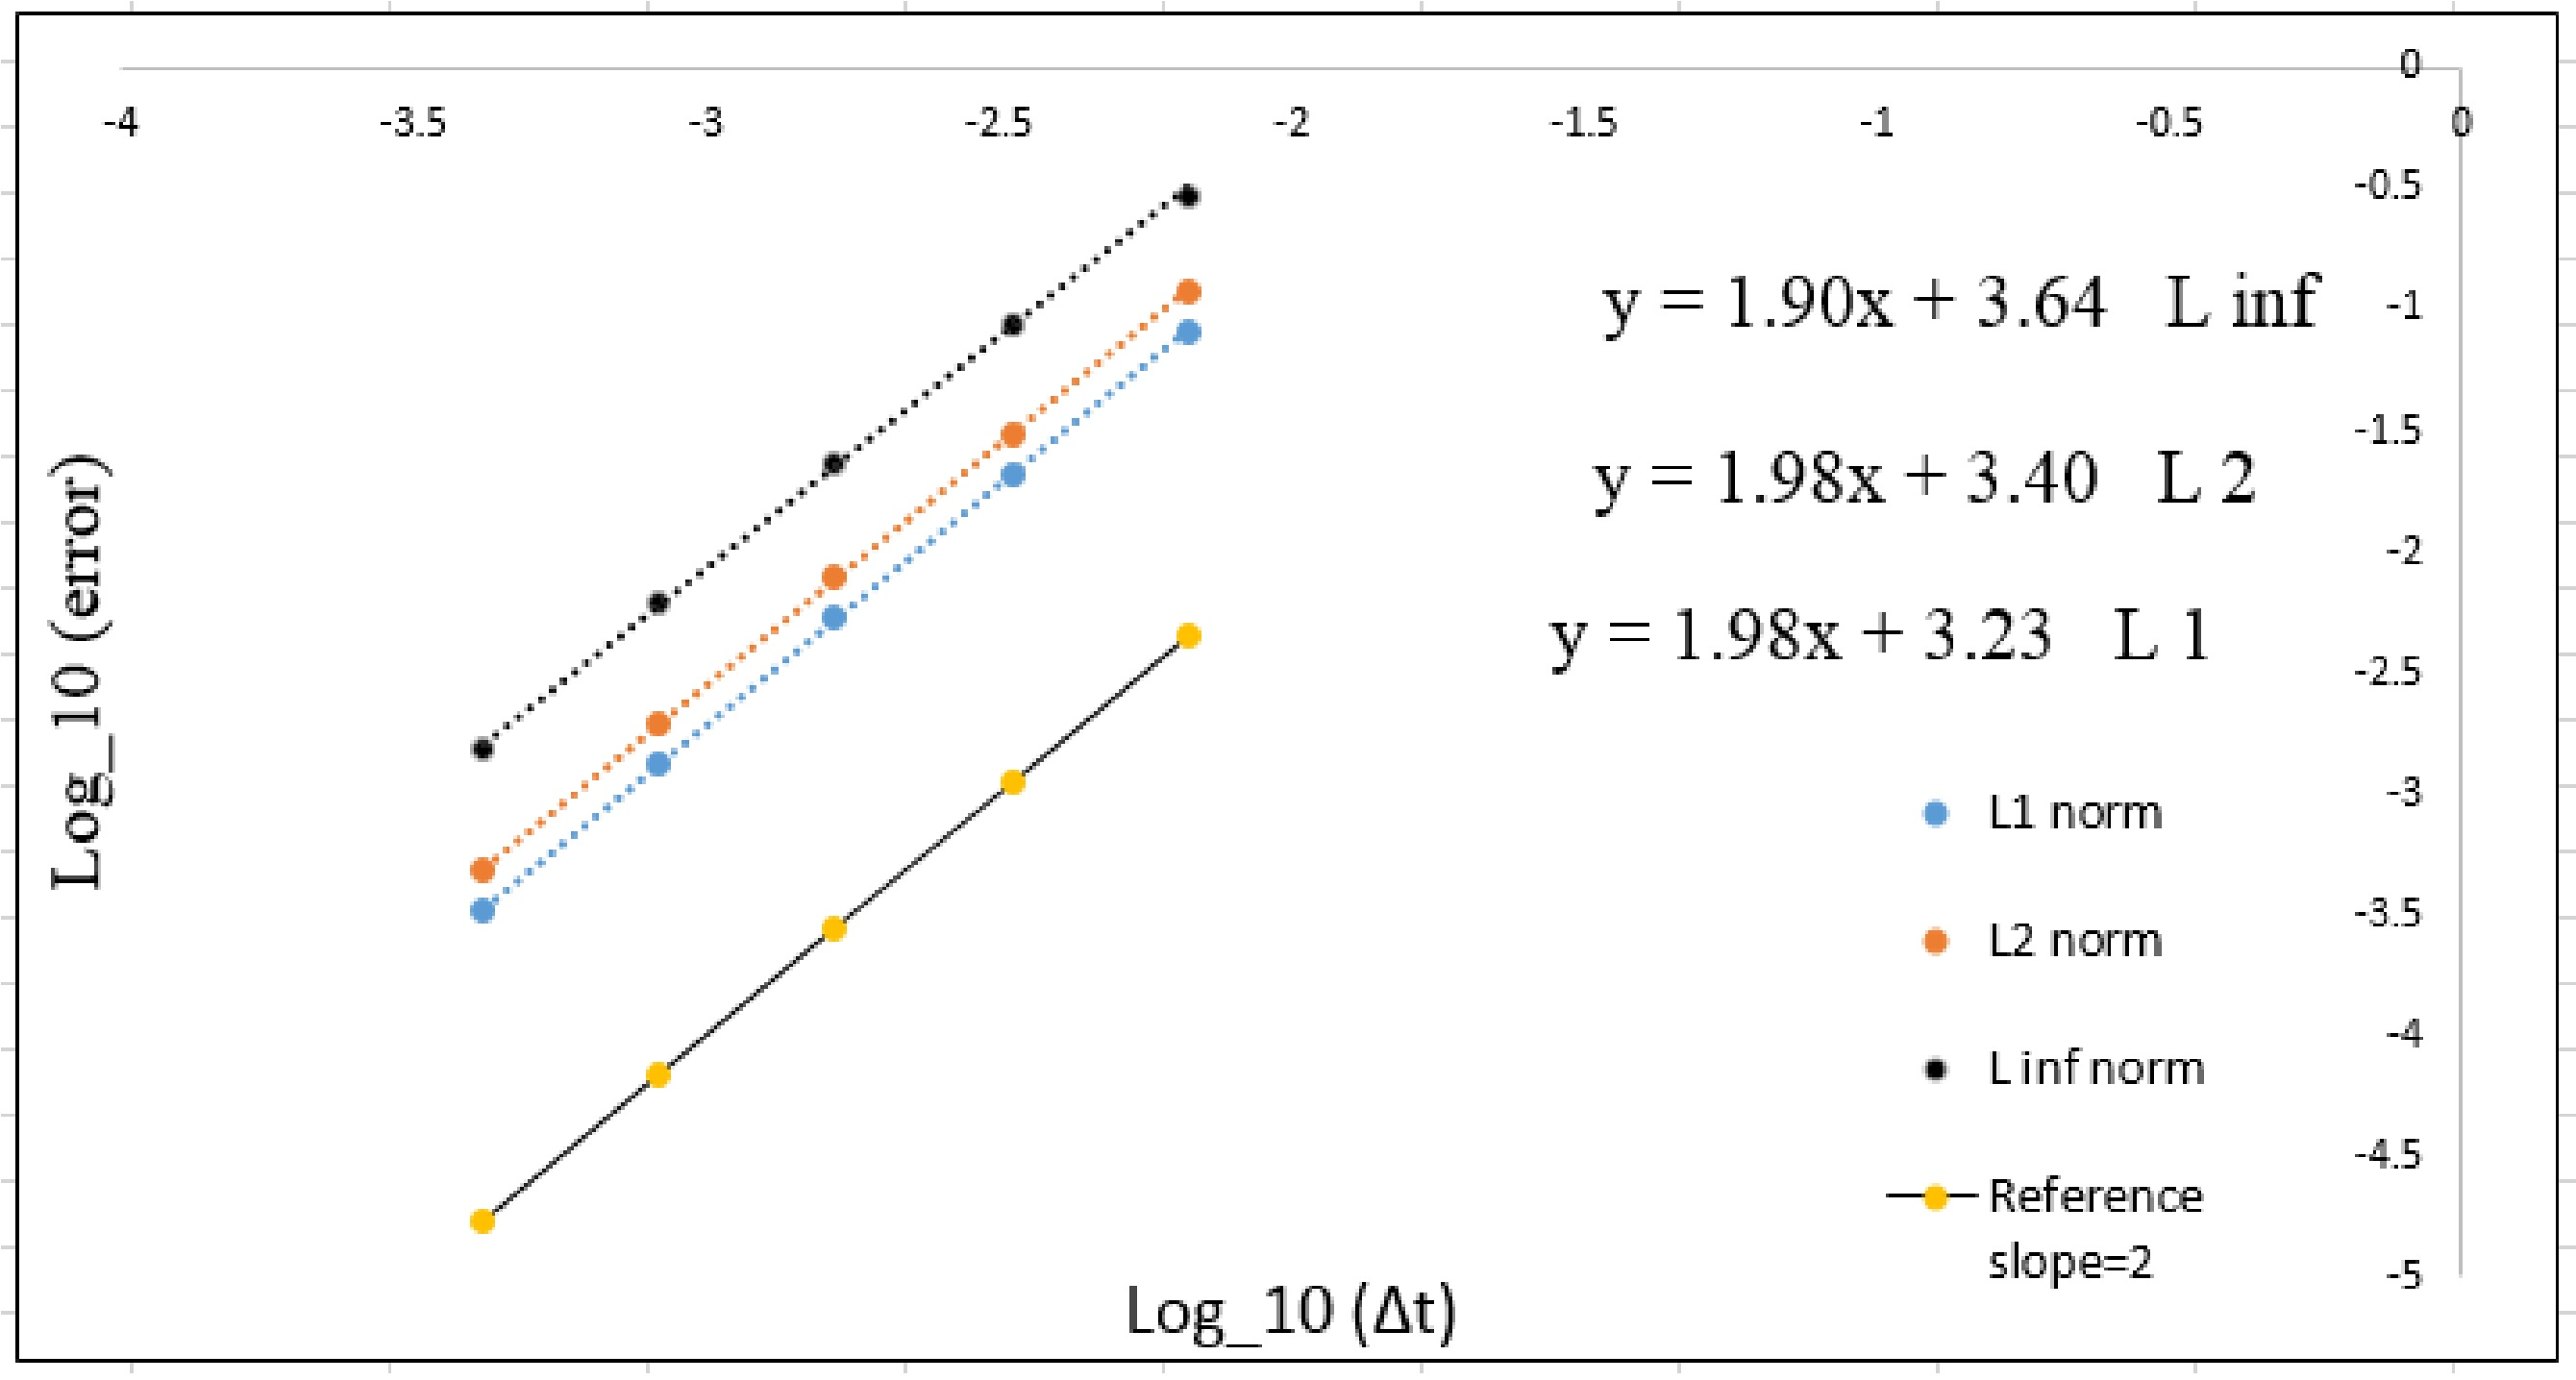
\includegraphics[width=4.5in]{C:/Users/HONGJI/Latex Home directory/Pm2_pf2b_np_P_rate_c_0_5.jpg}}
		\caption{Log-Log plot of Convergence rate for Pressure}\label{fig:6.19a}		
	\end{subfigure}
	\quad
	\begin{subfigure}[t]{4.5in}
		\centering
		\scalebox{1.2}{
		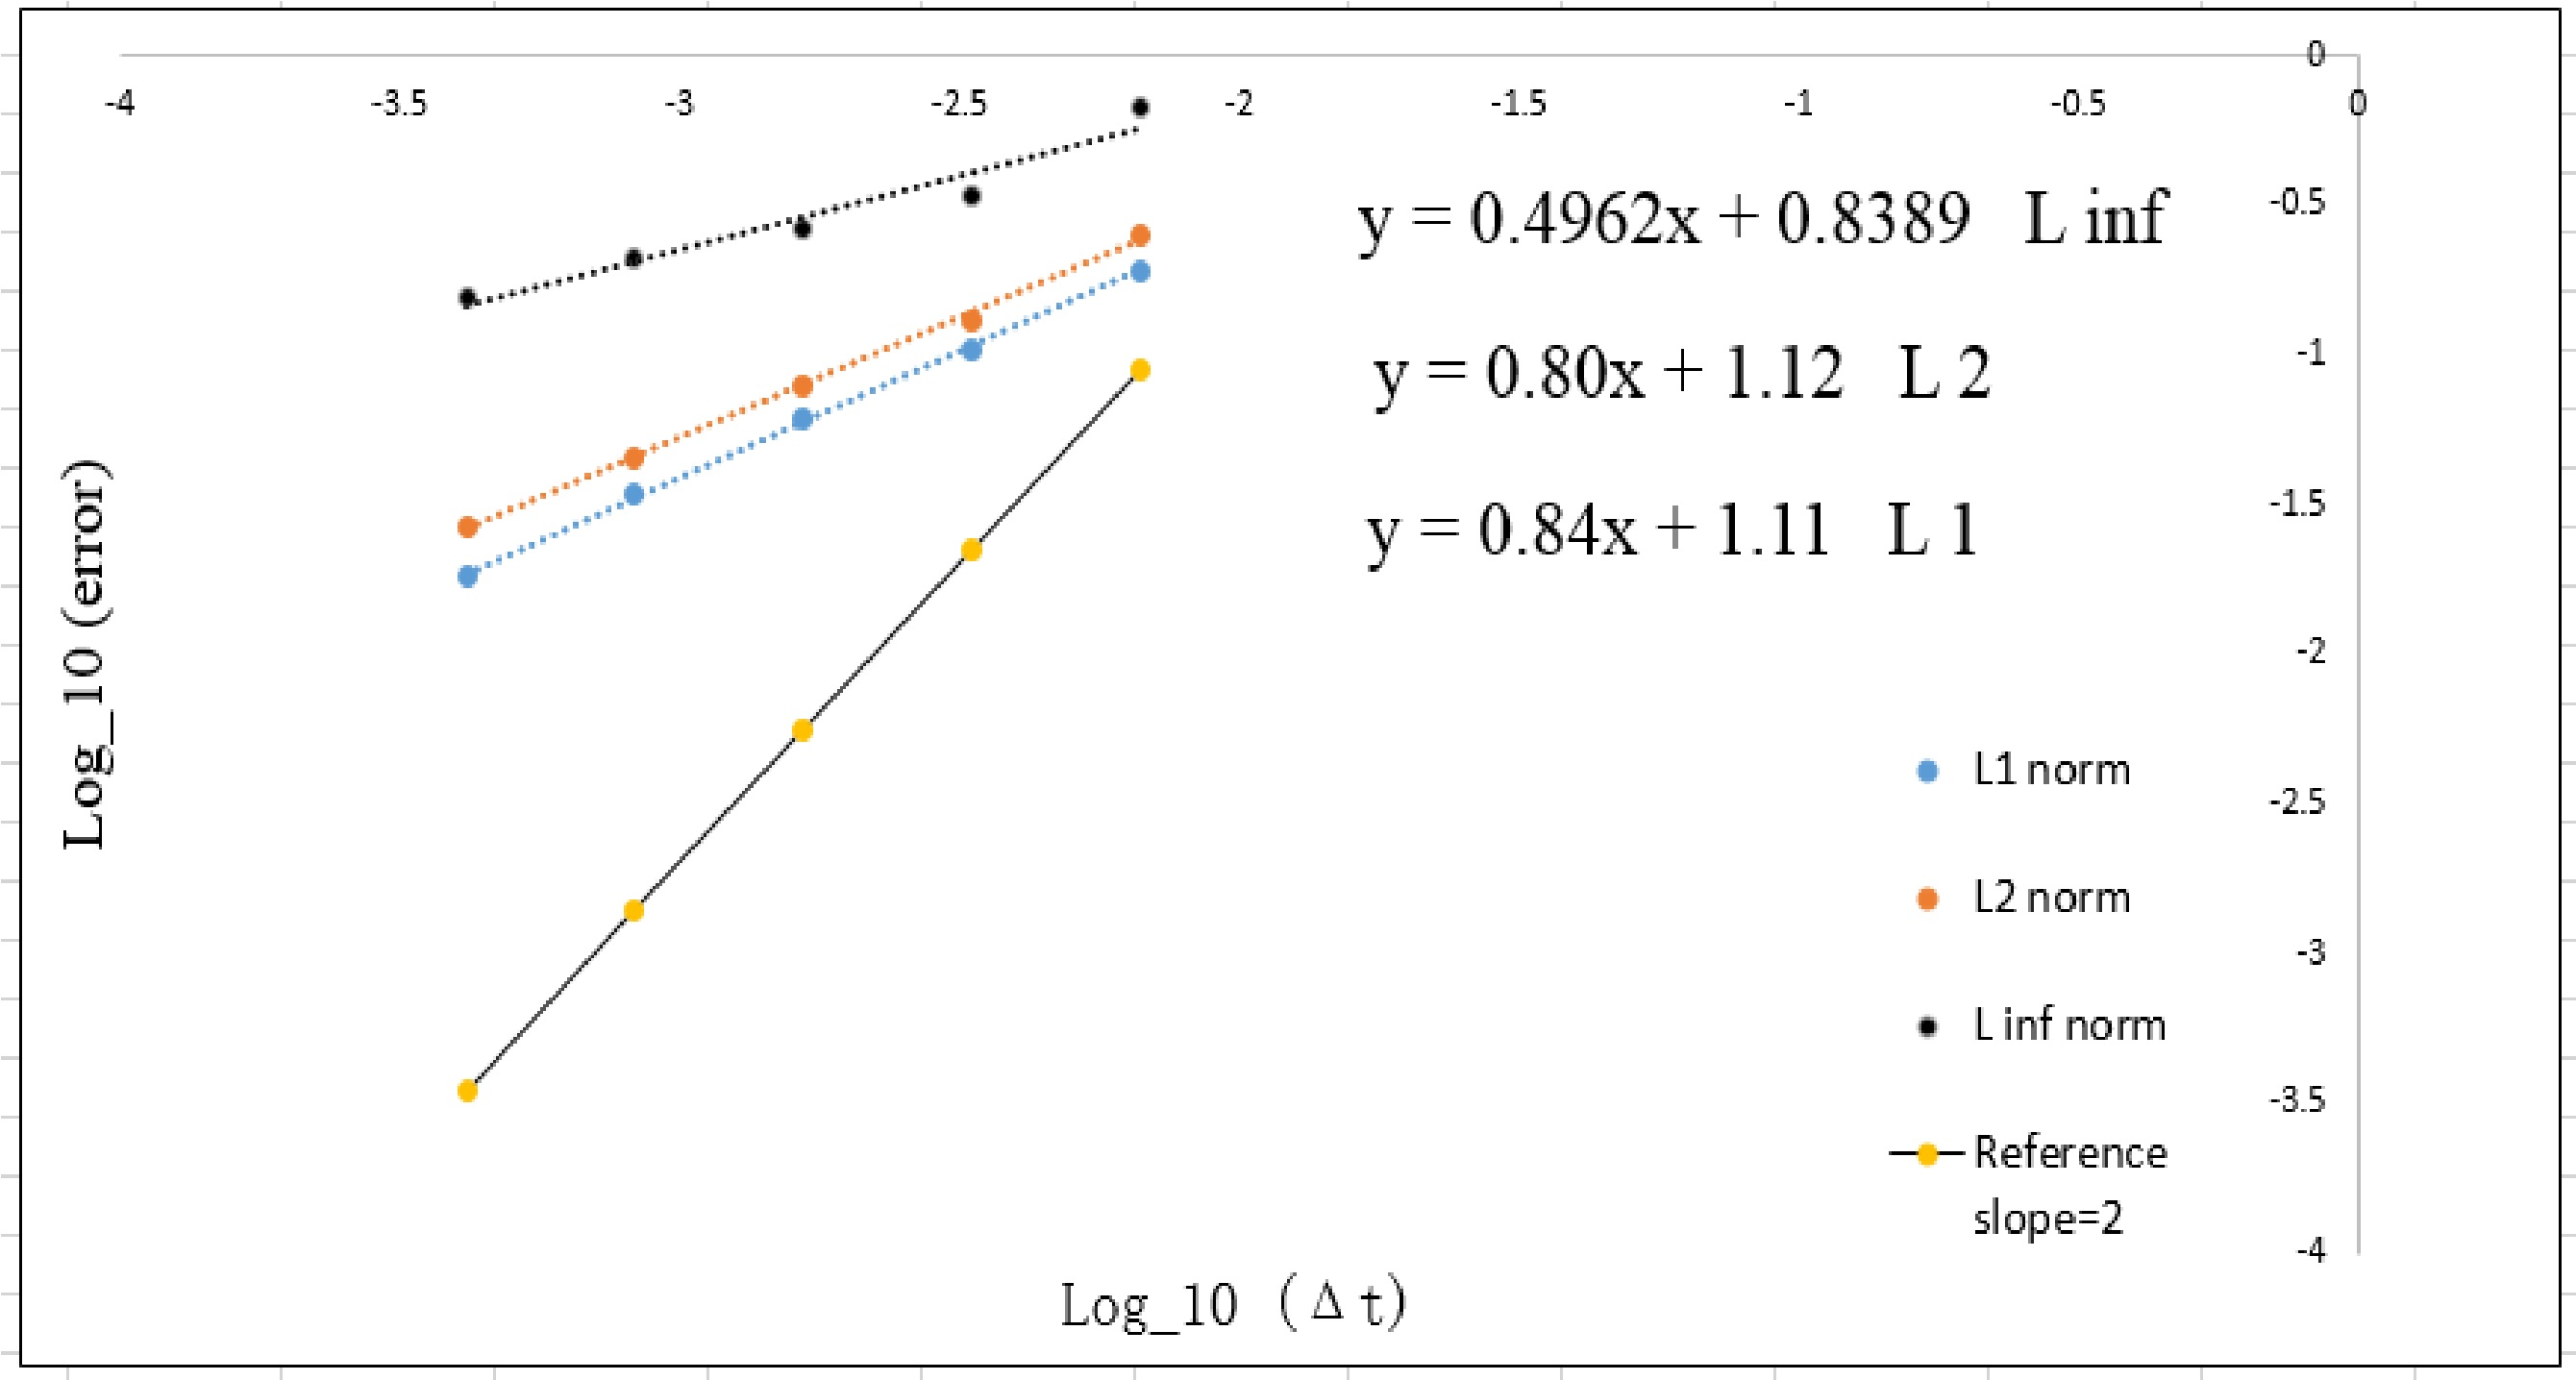
\includegraphics[width=4.5in]{C:/Users/HONGJI/Latex Home directory/Pm2_pf2b_np_div_uvstar_rate_c_0_5.jpg}}
		\caption{Log-Log plot of Convergence rate for $\nabla \cdot \textbf{u}^*$. }\label{fig:6.19b}
	\end{subfigure}
	\caption{Plot of Convergence rates for Alg 3. Domain: $[-\dfrac{1}{2}, \dfrac{1}{2}]^2$, time = 1 and CFL = 0.5. In each plot, the data points corresponding to grid sizes of 15, 30, 60, 120, 240.}\label{fig:6.16}
\end{figure}

\begin{figure}[H]
	\centering
	\scalebox{1.2}{
	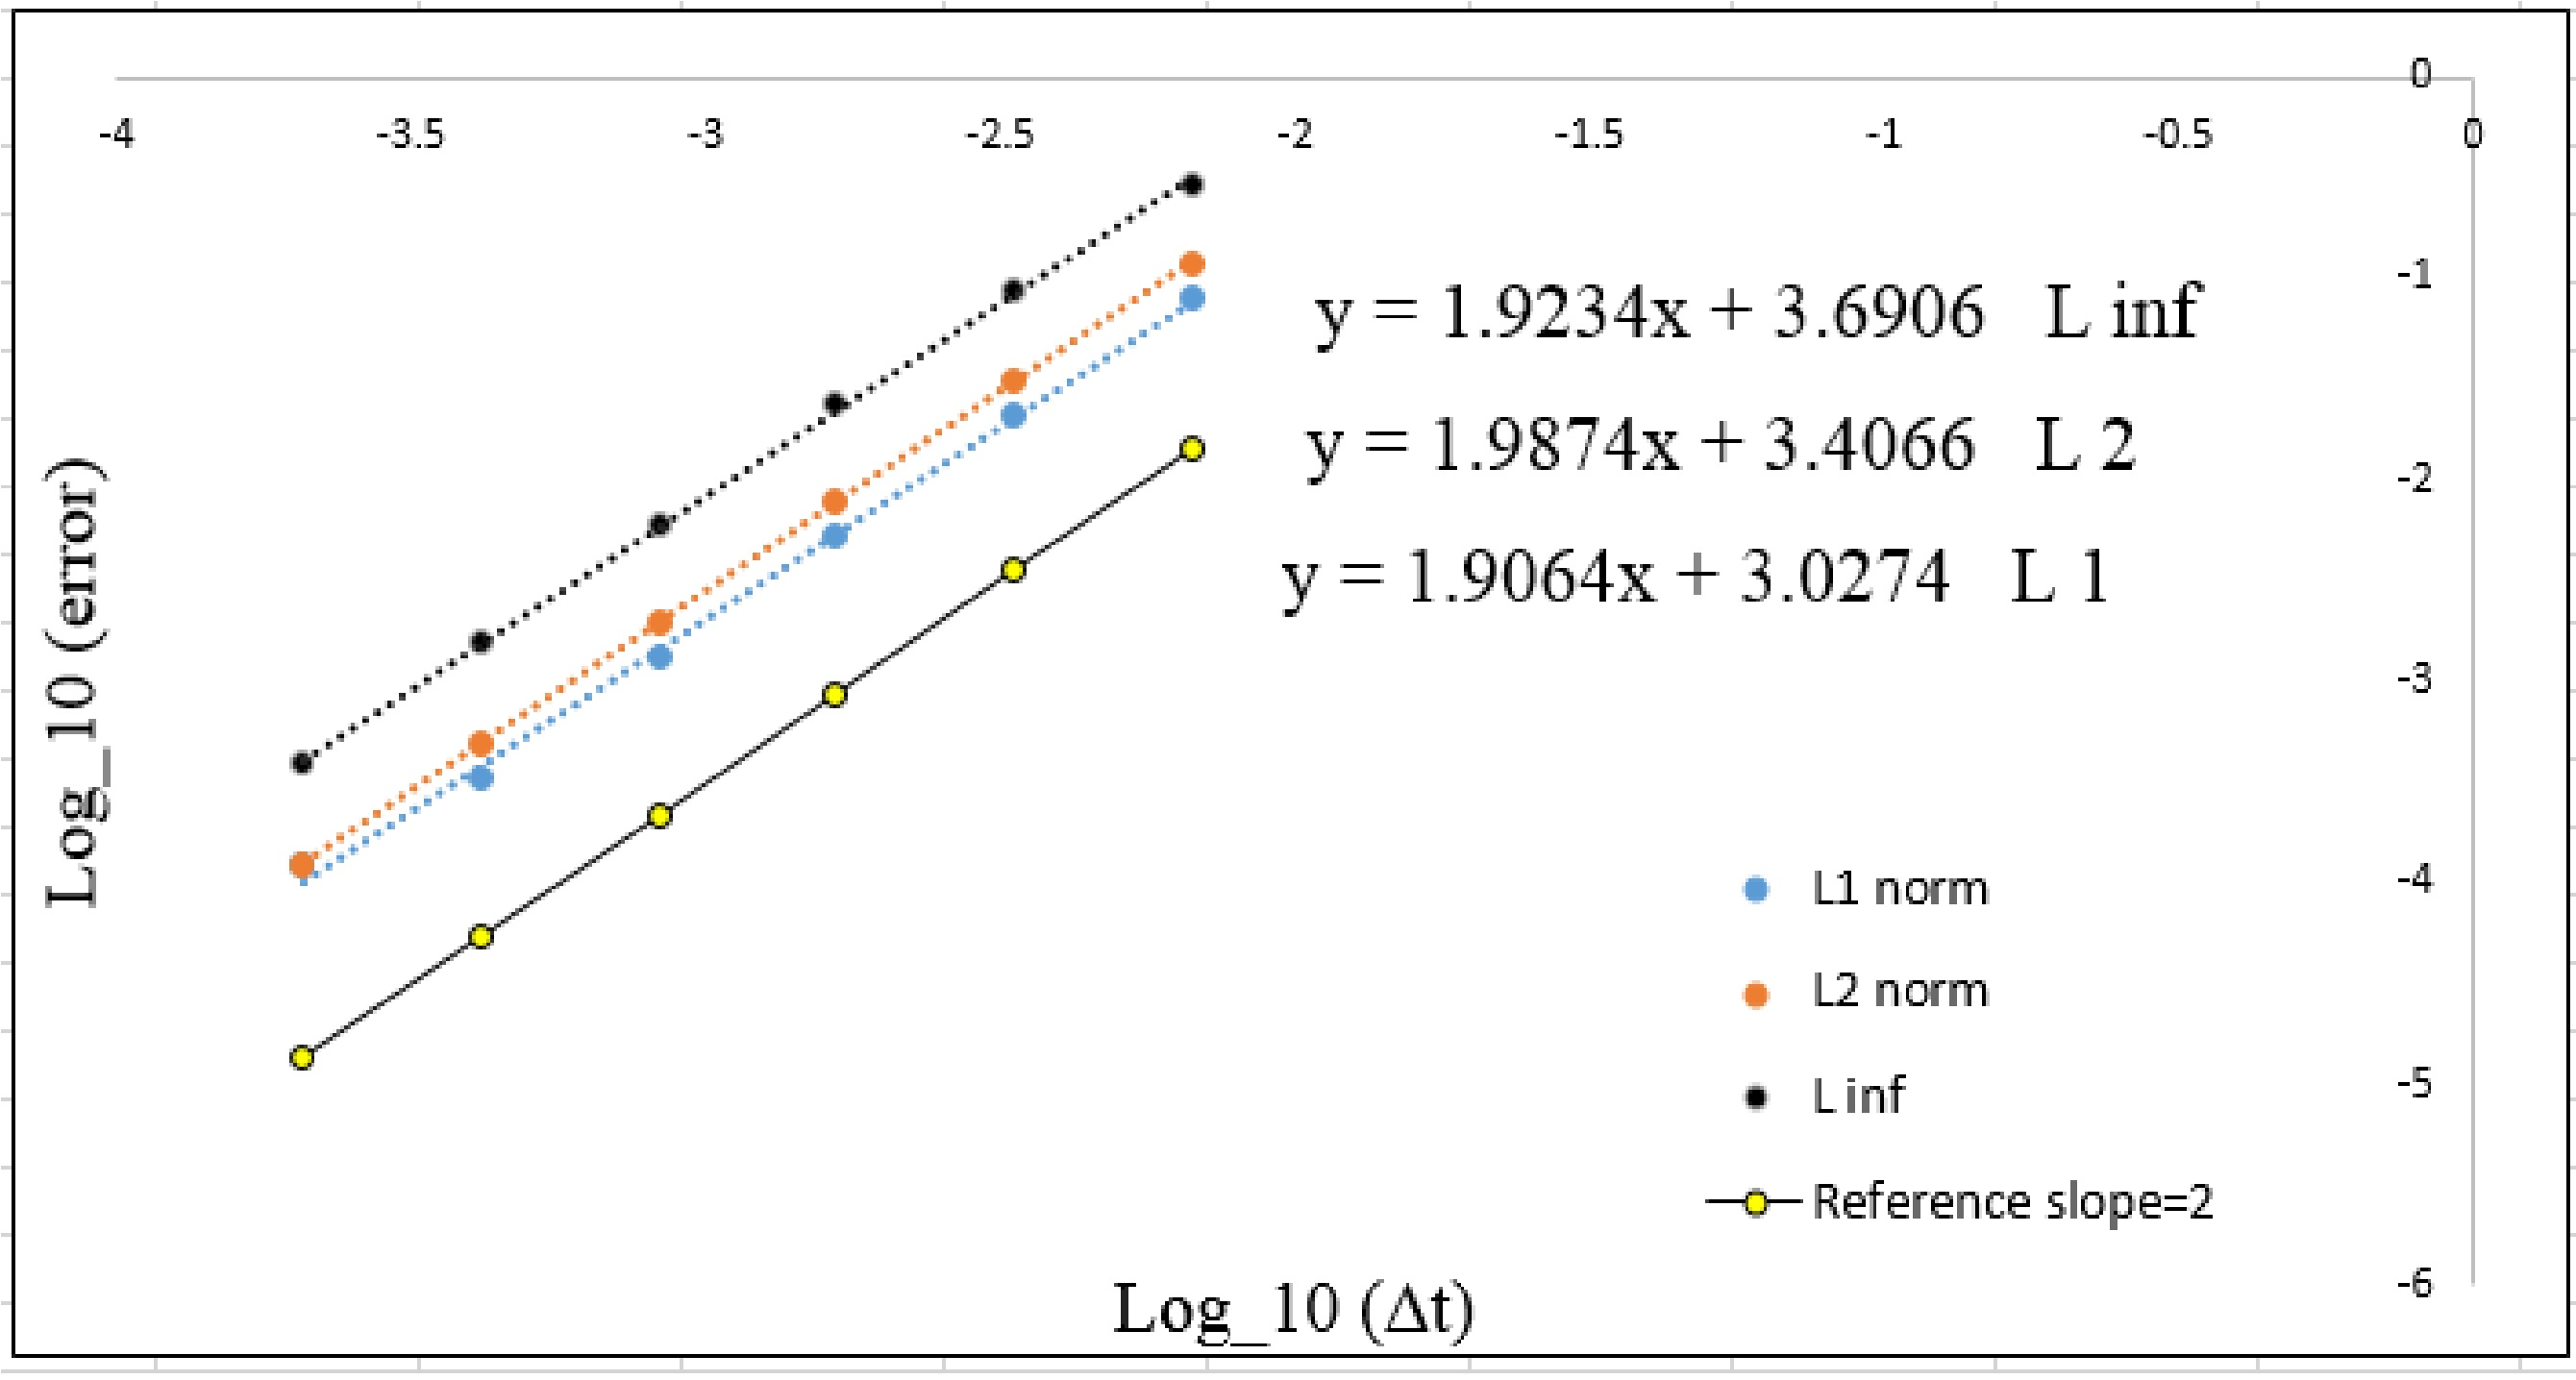
\includegraphics[width=4.5in]{C:/Users/HONGJI/Latex Home directory/Gauge_pf2b_np_P_rate_c_0_5.jpg}}
	\caption{Long-Log plot of Pressure Convergence rates for Gauge method. Domain: $[-\dfrac{1}{2},\dfrac{1}{2}]^2$, time = 1 and CFL = 0.5. The data points corresponding to grid sizes of 15, 30, 60, 120, 240, and 480.}\label{fig:6.16}
\end{figure}

\begin{figure}[H]
	\centering
	\begin{subfigure}[t]{2.2in}
		\centering
		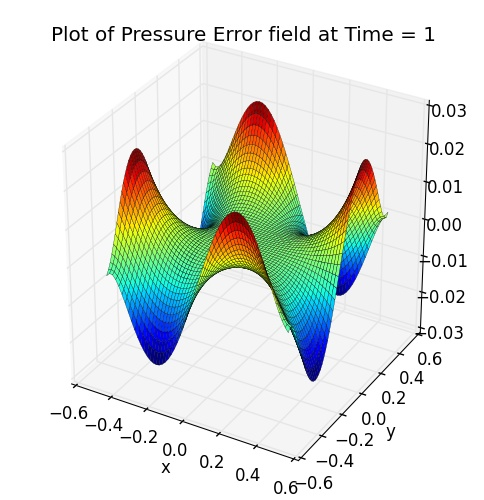
\includegraphics[width=2.2in]{C:/Users/HONGJI/Latex Home directory/Pm1b_pf2b_P_error_t_1_grid_60.jpg}
		\caption{Pressure error field for Alg 2 method}\label{fig:6.19a}		
	\end{subfigure}
	\quad
	\begin{subfigure}[t]{2.6in}
		\centering
		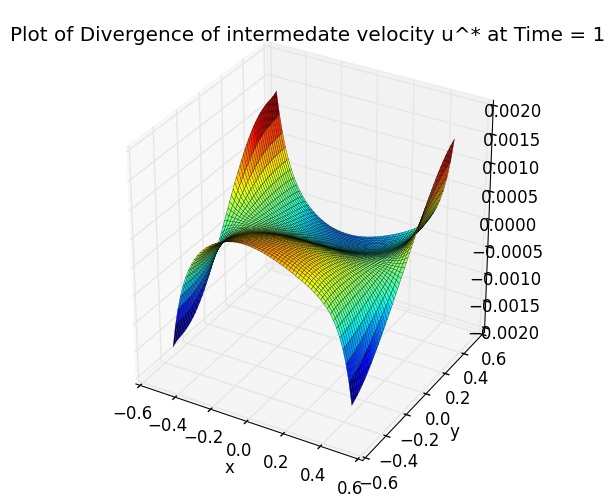
\includegraphics[width=2.6in]{C:/Users/HONGJI/Latex Home directory/Pm1b_pf2b_div_uvstar_t_1_grid_60.jpg}
		\caption{Divergence of intermediate velocity field for Alg 2 method. }\label{fig:6.19b}
	\end{subfigure}
	\quad
	\centering
	\begin{subfigure}[t]{2.2in}
		\centering
		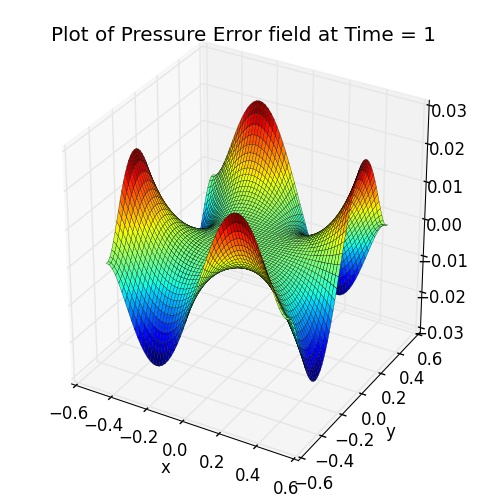
\includegraphics[width=2.2in]{C:/Users/HONGJI/Latex Home directory/Pm2_pf2b_np_P_error_t_1_grid_60.jpg}
		\caption{Pressure error field for Alg 3 method}\label{fig:6.19c}		
	\end{subfigure}
	\quad
	\begin{subfigure}[t]{2.6in}
		\centering
		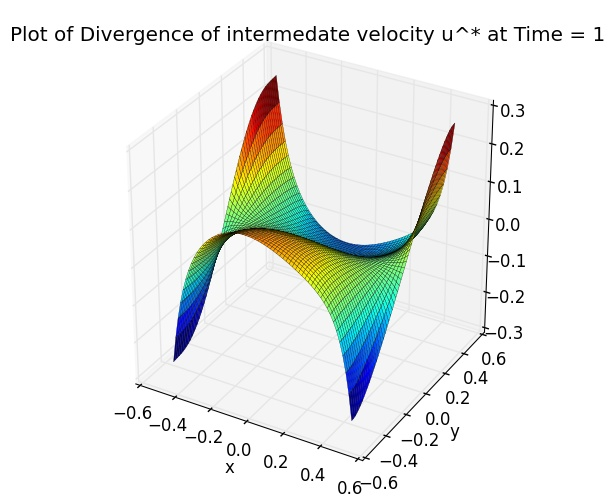
\includegraphics[width=2.6in]{C:/Users/HONGJI/Latex Home directory/Pm2_pf2b_np_div_uvstar_t_1_grid_60.jpg}
		\caption{Divergence of intermediate velocity field for Alg 3 method.}\label{fig:6.19d}
	\end{subfigure}
	\quad
	\begin{subfigure}[t]{2.5in}
		\centering
		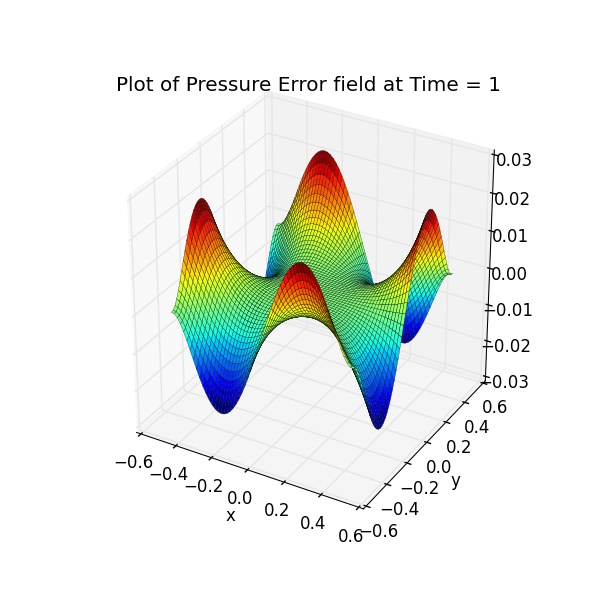
\includegraphics[width=2.5in]{C:/Users/HONGJI/Latex Home directory/Gauge_pf2b_P_error_t_1_grid_60_corrected.jpg}
		\caption{Pressure error field for Gauge method. }\label{fig:6.19d}
	\end{subfigure}
	\caption{Pressure error fields and divergence of intermediate velocity (if applicable) for Alg 2, Alg 3 and Gauge method at grid size of 120. Domain: $[-\dfrac{1}{2},\dfrac{1}{2}]^2$, time = 1 and CFL = 0.5. }\label{fig:6.16}
\end{figure}

\subsection*{Necessity for accurate approximation to $\phi^{n+1}$ along the tangential boundary of the intermediate velocity field.}
We investigate the importance of boundary condition choice for the intermediate velocity field and this might also help to understand why Alg 3 behaves better than Alg 2 in pressure convergence rates. We took two extrema here in choosing the tangential boundary condition for $\textbf{u}^*$: one is use second order approximation to $\phi^{n+1}$ so we have $\textbf{$\tau$} \cdot \textbf{u}^* \,|_{\partial \Omega} = \textbf{$\tau$} \cdot (\textbf{u}^{n+1} + \nabla (2\phi^n - \phi^{n-1})\,|_{\partial \Omega}$ (as of what we have done before for Alg 3); the other is to use no approximation to $\phi^{n+1}$. We now rerun Alg 3 with the less accurate boundary where $\textbf{$\tau$} \cdot \textbf{u}^* = \textbf{$\tau$} \cdot \textbf{u}^{n+1}$ (this is the same as Alg 2). The convergence rates in pressure are again summarised in Figure below. It is observed that the rates are much reduced to about 0.7 order. The plot of pressure error field also shows four spikes at corners as in Alg 2. Hence this indicate the choice of tangential boundary condition to $\textbf{u}^*$ does indeed affect the performance of numerical boundary layer elimination. This finding indicates that for Alg 3 accurate approximation to $\phi^{n+1}$ must be implemented when computing the intermediate velocity field along the boundary points. This is consistent with the predications of our normal mode analysis. It is also consistent with the findings of others \cite{brown2001accurate}. We infer that the same result might also work for Alg 2. However we did not have enough time to implement the different condition for Alg 2.

\begin{figure}[H]
	\centering
	\scalebox{1.5}{
	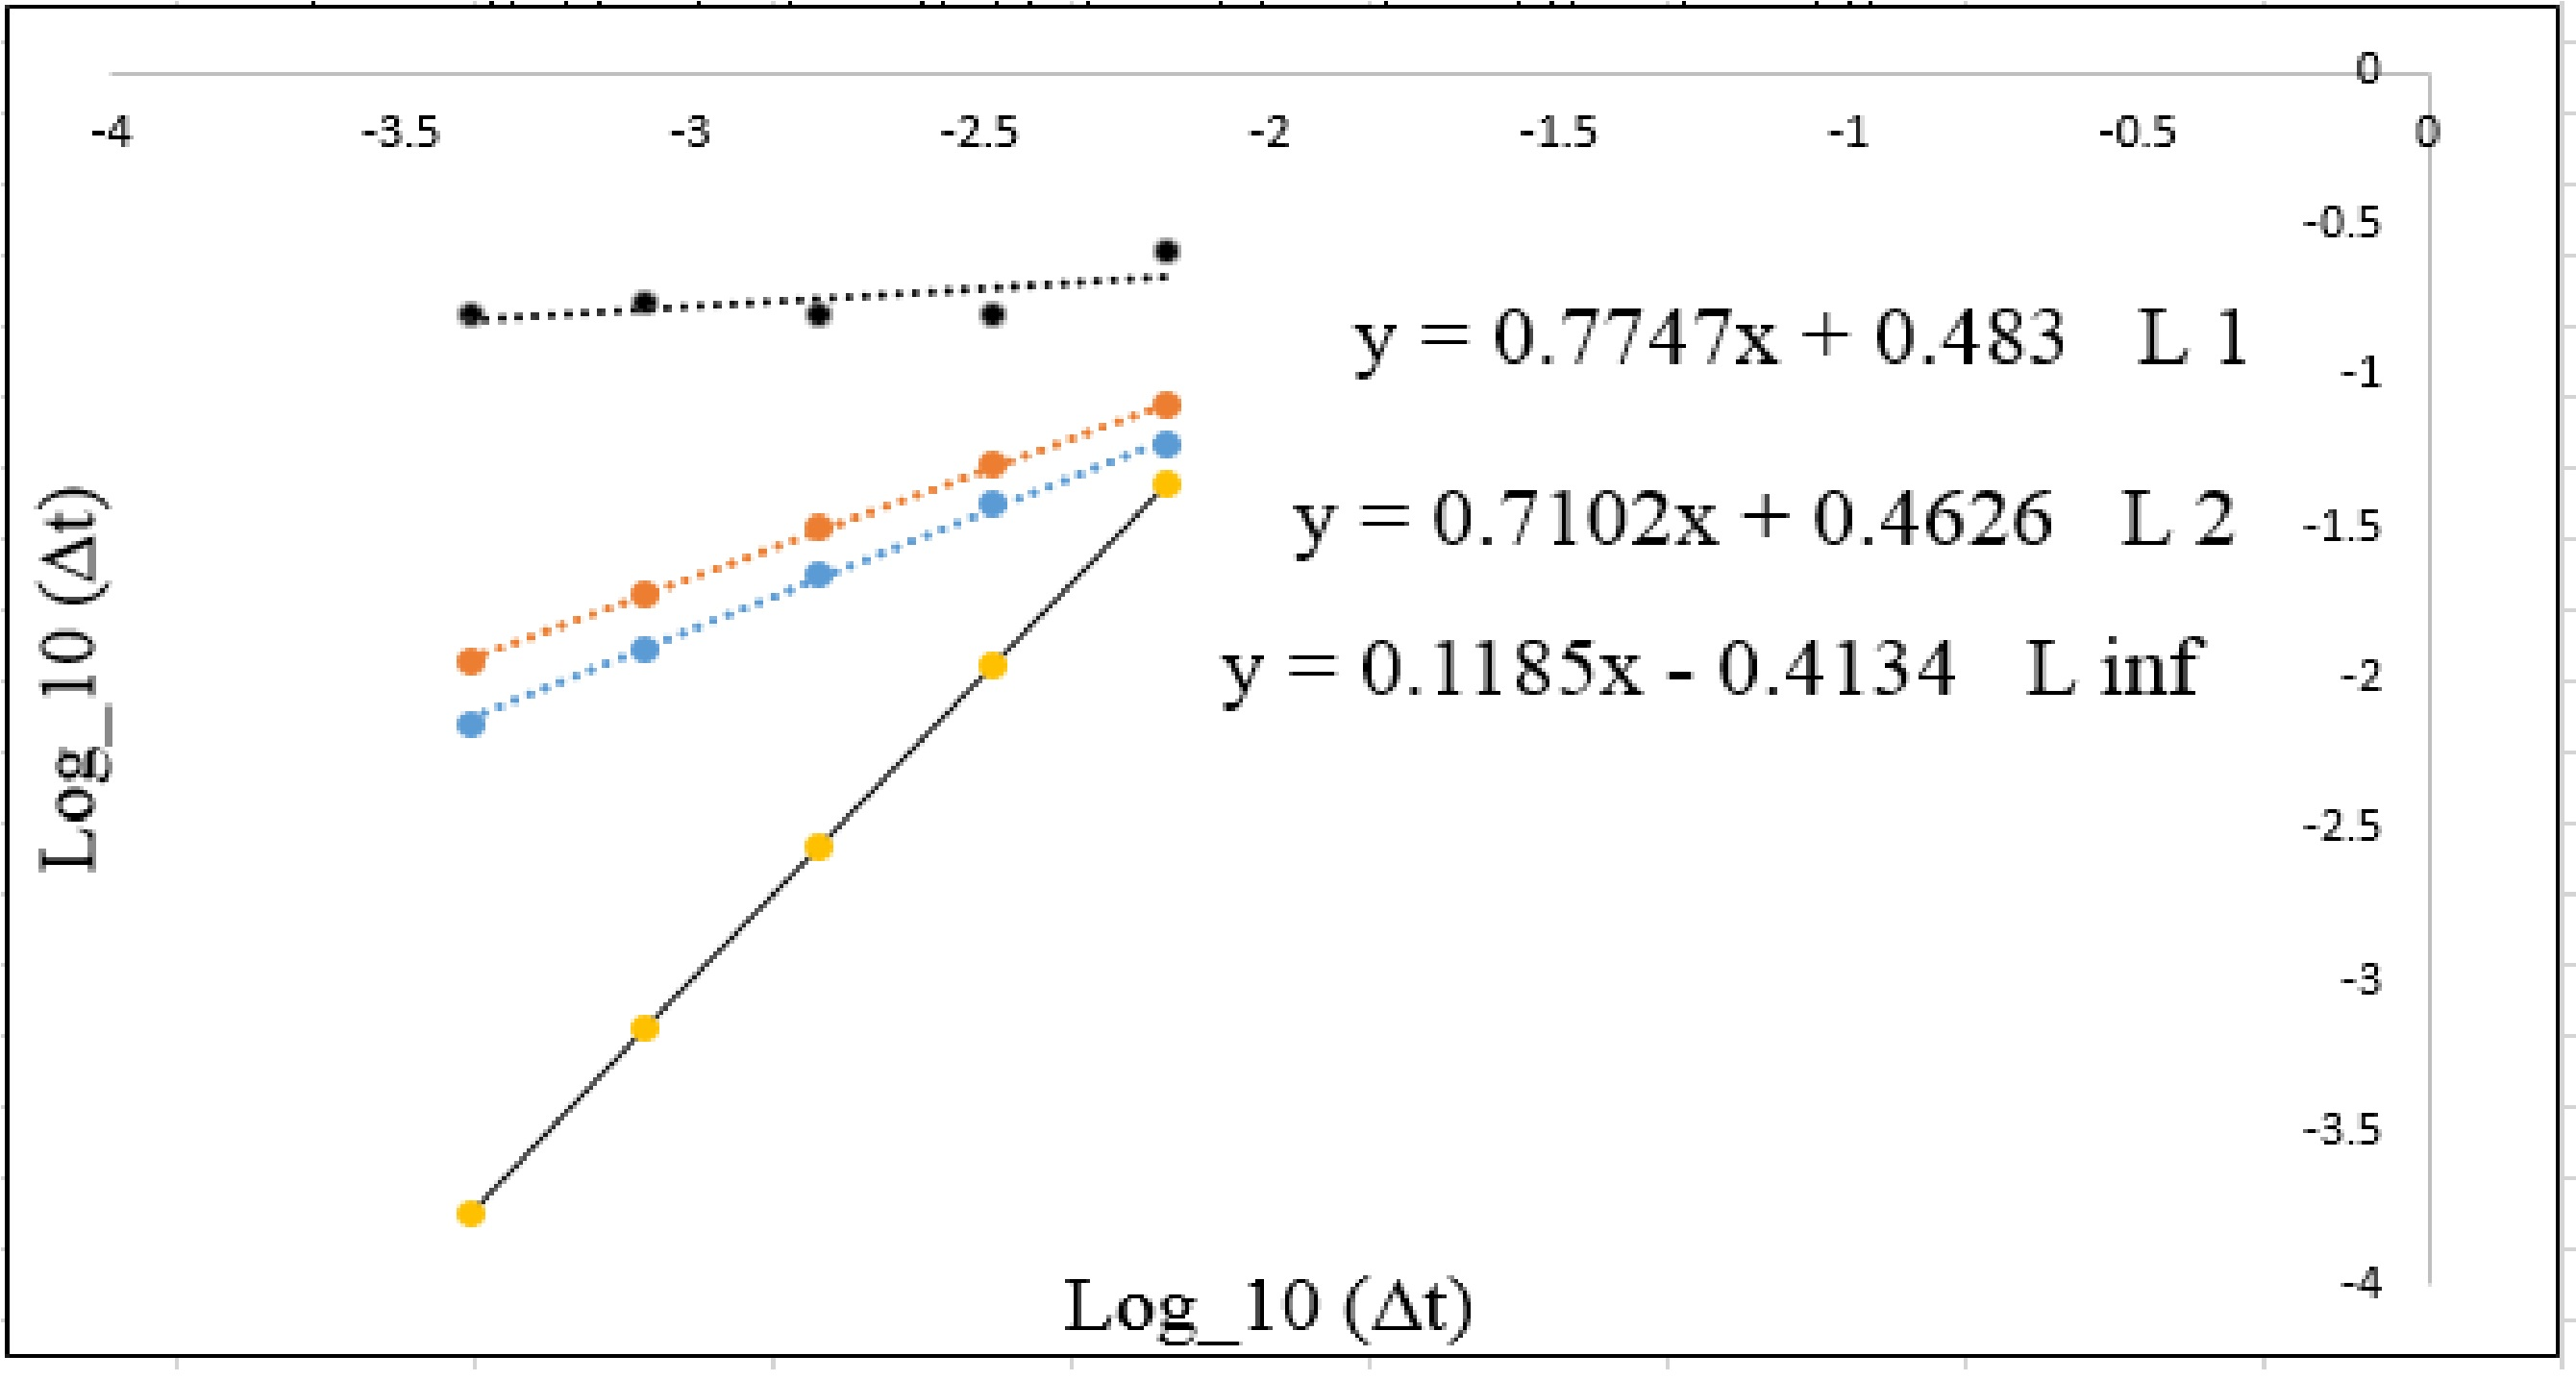
\includegraphics[width=3.5in]{C:/Users/HONGJI/Latex Home directory/Pm2D_pf2_p_rate_cfl_0_5.jpg}}
	\caption{Log log plot of pressure error convergence rate for Alg 3 with less accurate boundary condition for $\nabla \cdot \textbf{u}^*$. }\label{fig:6.20}
\end{figure}
	
\begin{figure}[H]
	\begin{subfigure}[t]{2.6in}
		\centering
		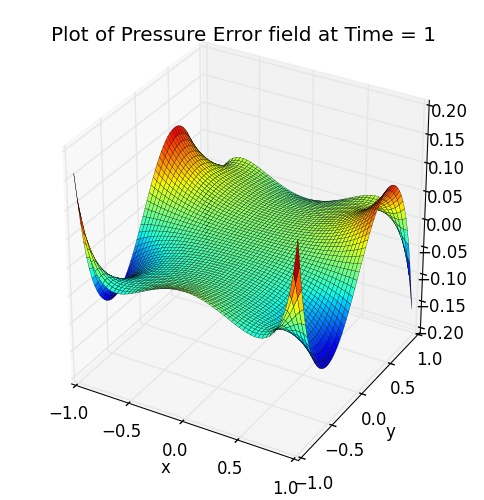
\includegraphics[width=2.6in]{C:/Users/HONGJI/Latex Home directory/Pm2D_pf2_np_P_error_t_1_grid_60.jpg}
		\caption{Pressure error field for Alg 3 with grid size 60 at time 1. }\label{fig:6.19b}
	\end{subfigure}
	\begin{subfigure}[t]{3.0in}
		\centering
		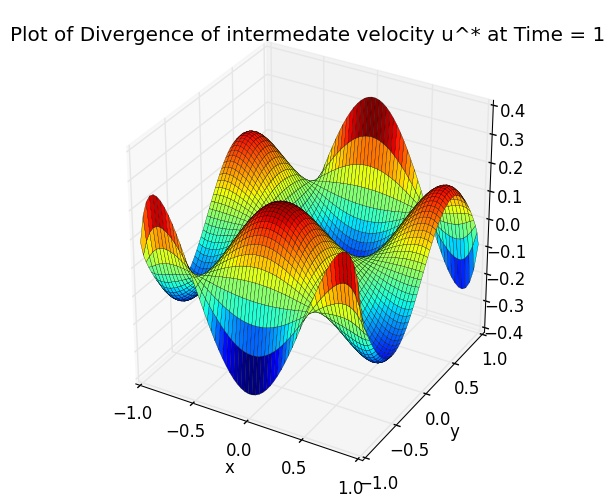
\includegraphics[width=3.0in]{C:/Users/HONGJI/Latex Home directory/Pm2D_pf2_np_div_uvstar_t_1_grid_60.jpg}
		\caption{Plot of $\nabla \cdot \textbf{u}^*$ for Alg 3 with grid size 60 at time 1. }\label{fig:6.19b}
	\end{subfigure}
	\caption{Long-Log plot of Pressure Convergence rates and $3D$ surface plot of pressure error field for Alg 3 where the less accurate tangential boundary is used. Domain: $[-1,1]^2$, time = 1 and CFL = 0.5. The data points corresponding to grid sizes of 15, 30, 60, 120, 240.}\label{fig:6.19c}
\end{figure}

\newpage
\subsection{Unforced flow problem}

To test the effect of smoothness of domain to the accuracy of projection methods. Another unforced flow problem is also considered. It is the well-known 2-D Taylor solution to the Navier Stokes equations. The analytic solutions are:

\begin{dgroup}
\begin{dmath}
u = -\cos(x)\sin(y)e^{-2t}
\end{dmath}
\begin{dmath}
v = \sin(x)\cos(y)e^{-2t}
\end{dmath}
\begin{dmath}
p = -\dfrac{1}{4\,R}(\cos(2x)+\cos(2y))e^{-4t}
\end{dmath}
\end{dgroup}

This test problem has non-zero boundary conditions for velocities and non-zero pressure gradients, unlike the forced flow exampled we have considered before where 2 of its boundaries are zero for velocities and pressure. Hence this should reveal more information on how the projection methods depends on the structure of domain and boundary conditions. For simplicity let's consider the domain: $[-\dfrac{\pi}{4}, \dfrac{\pi}{4}]^2$. Then the pressure value at these 4 corners ($x = \pm \dfrac{\pi}{4}$ and $y = \pm \dfrac{\pi}{4}$) would then be zero for all times which makes our pressure normalisation process easier.\\

In addition, this Taylor solutions are derived from the full Navier Stokes equations and hence it is also good to test our convective term solvers too.\\

We have again run the Projection methods and Gauge for 5 grid sizes from $15 \times 15$ to $240 \times 240$. The spatial stepping is halved each time. The solutions are calculated at time 1s and with Reynolds number equals to 1. A CFL number of 0.5 is used in all methods to obtain better error estimates.\\

The convergence rates in pressure are summarised in Figure. Interestingly all the methods show fully second order convergence except for Alg 2 where only first order convergence is observed. This time all the norms show degraded accuracy. Take a look at the Pressure error field we observe very large spikes located at the 4 corners of the domain. This indicates the Presence of numerical boundary layers which are manifested better in the plot of Divergence of intermediate velocity field. Interestingly the magnitude of divergence of numerical boundary in intermediate velocity field is even larger for Alg 3 yet resulting in small Pressure error field. This result shows that the numerical boundary layers in $\phi$ and $\nabla \cdot \textbf{u}^*$ cannot be fully filtered out in the projection methods unless accurate boundary condition for $\textbf{$\tau$} \cdot \textbf{u}^*$ is implemented, same finding that supports the necessity for accurate tangential boundary condition for the intermediate velocity field. This is illustrated by the surface plots in Alg 2 where the thick boundary layer in $\nabla \cdot \textbf{u}^*$ is eliminated in Pressure but the 4 spikes still present. This finding is also consistent with that obtained in David's paper \cite{brown2001accurate}.\\

\begin{figure}[H]
	\centering
	\begin{subfigure}[t]{4.5in}
		\centering
		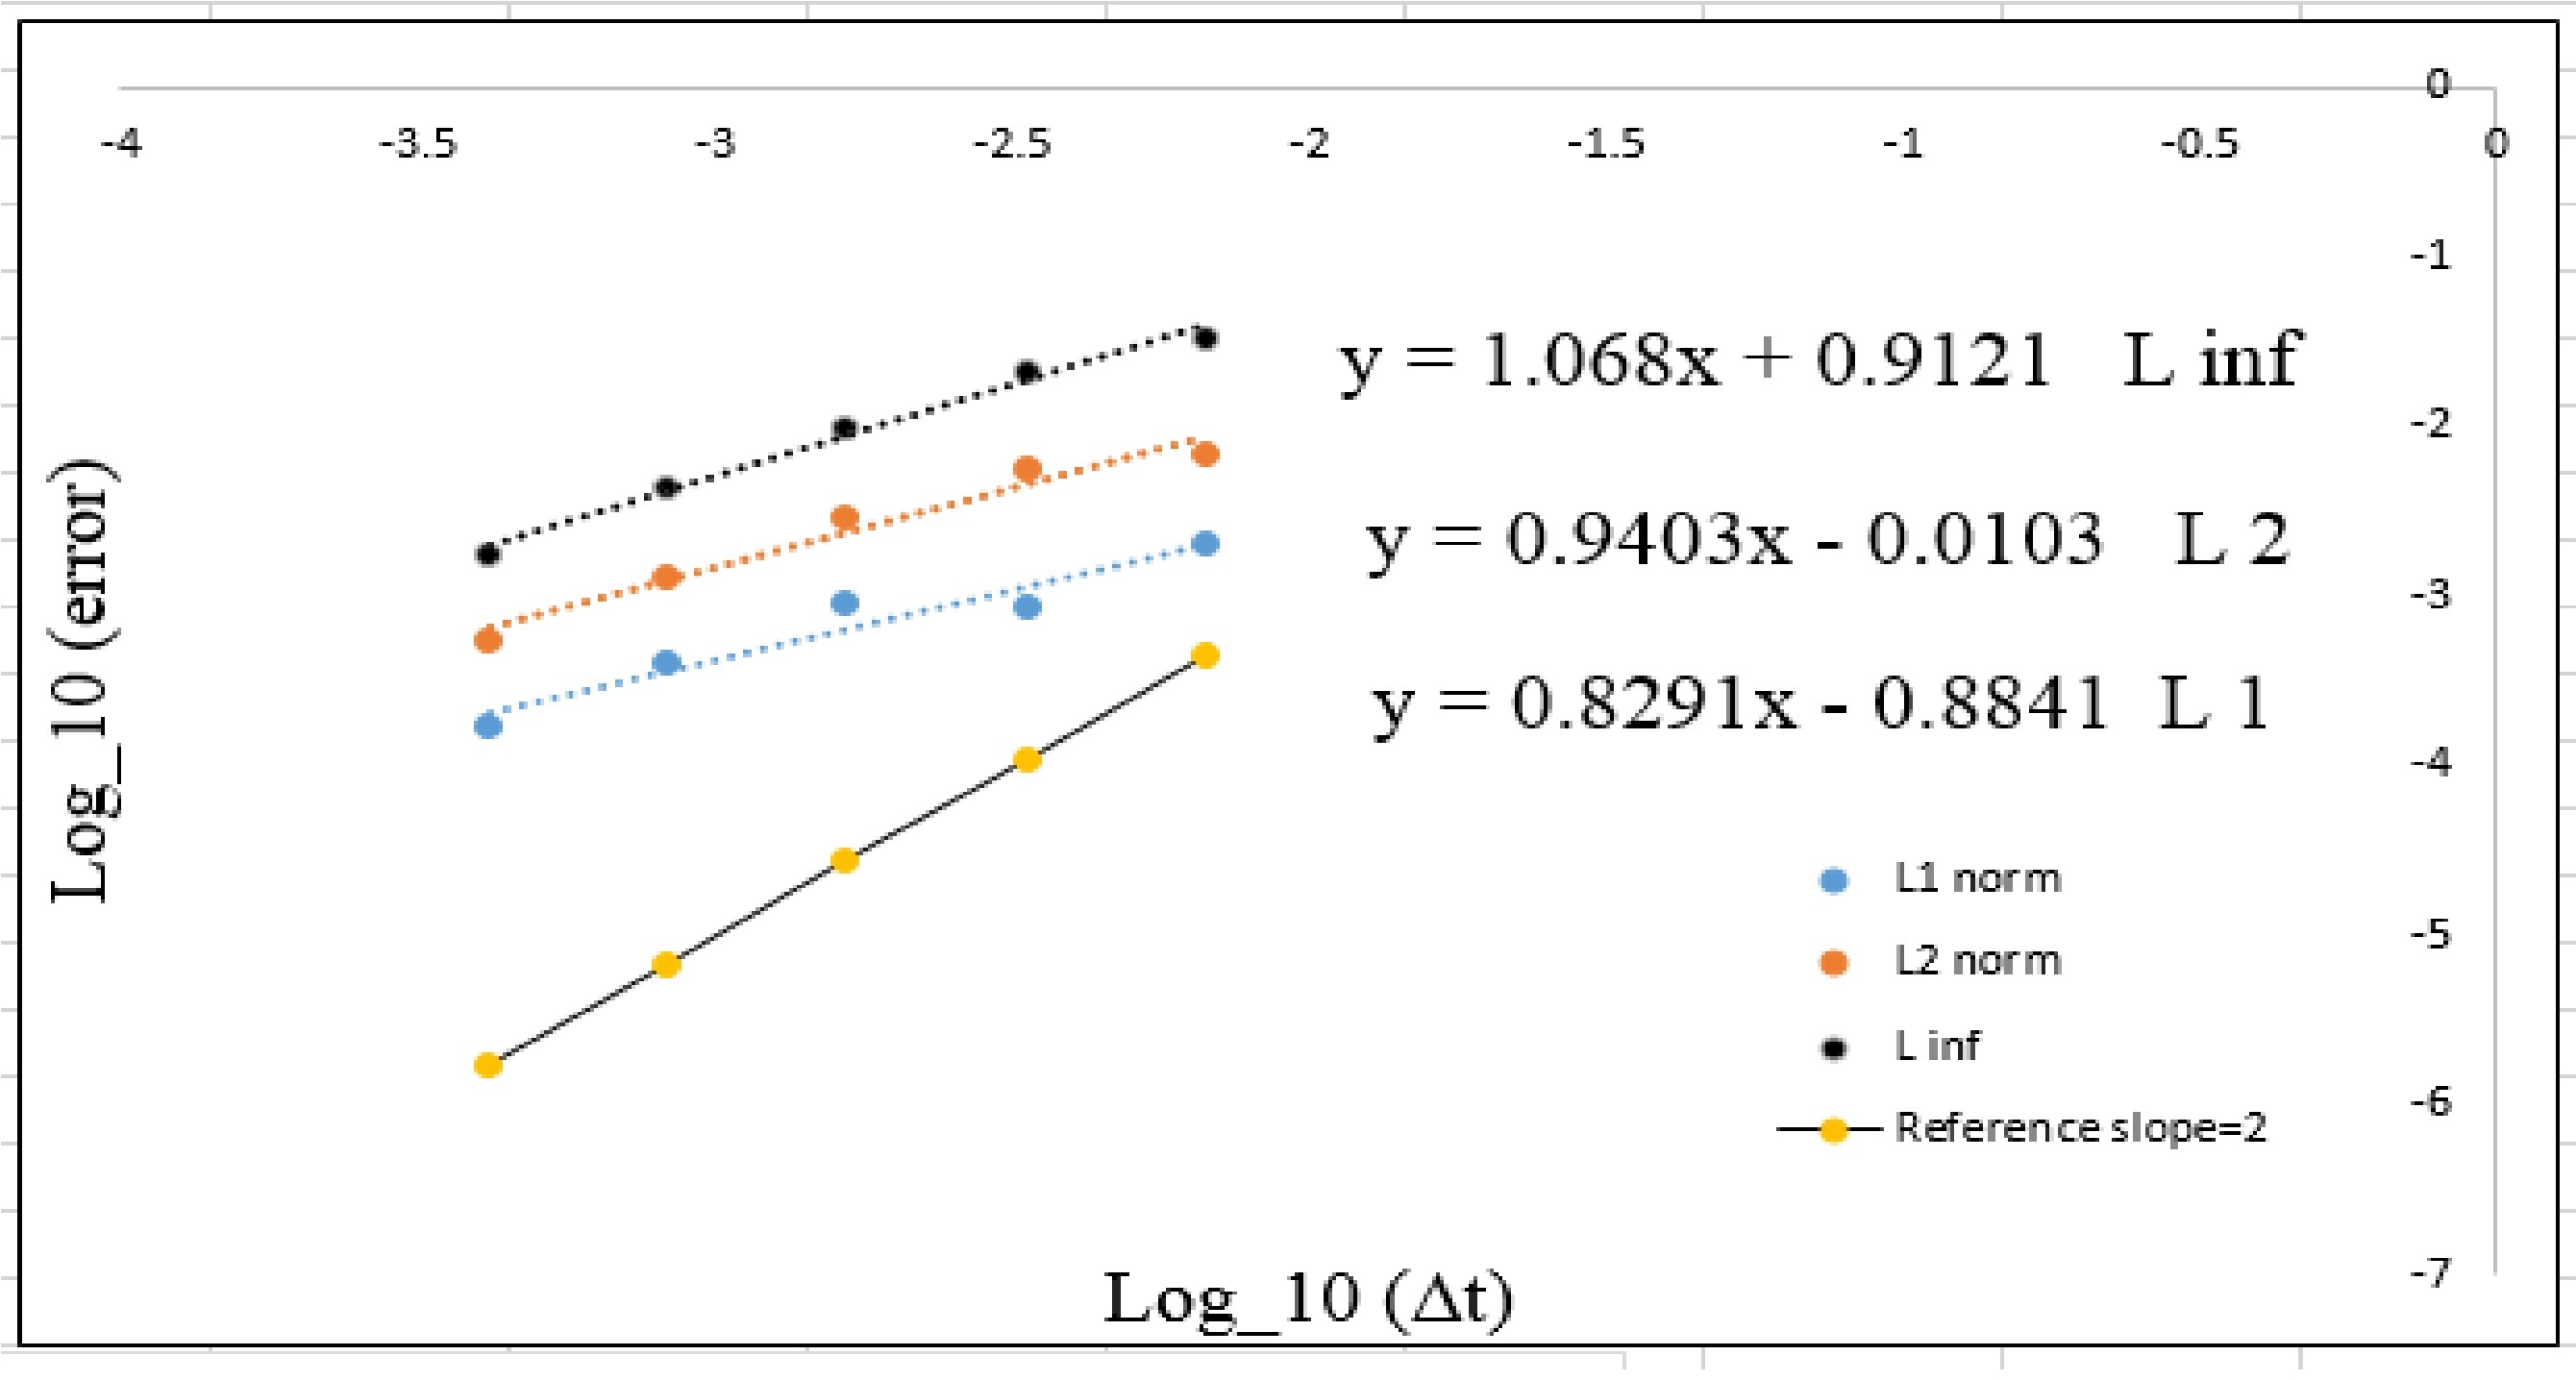
\includegraphics[width=4.5in]{C:/Users/HONGJI/Latex Home directory/Pm1b_unf1_np_P_rate.jpg}
		\caption{Log-Log plot of Convergence rate for Pressure Alg 2 method}\label{fig:6.19a}		
	\end{subfigure}
	\quad
	\begin{subfigure}[t]{4.5in}
		\centering
		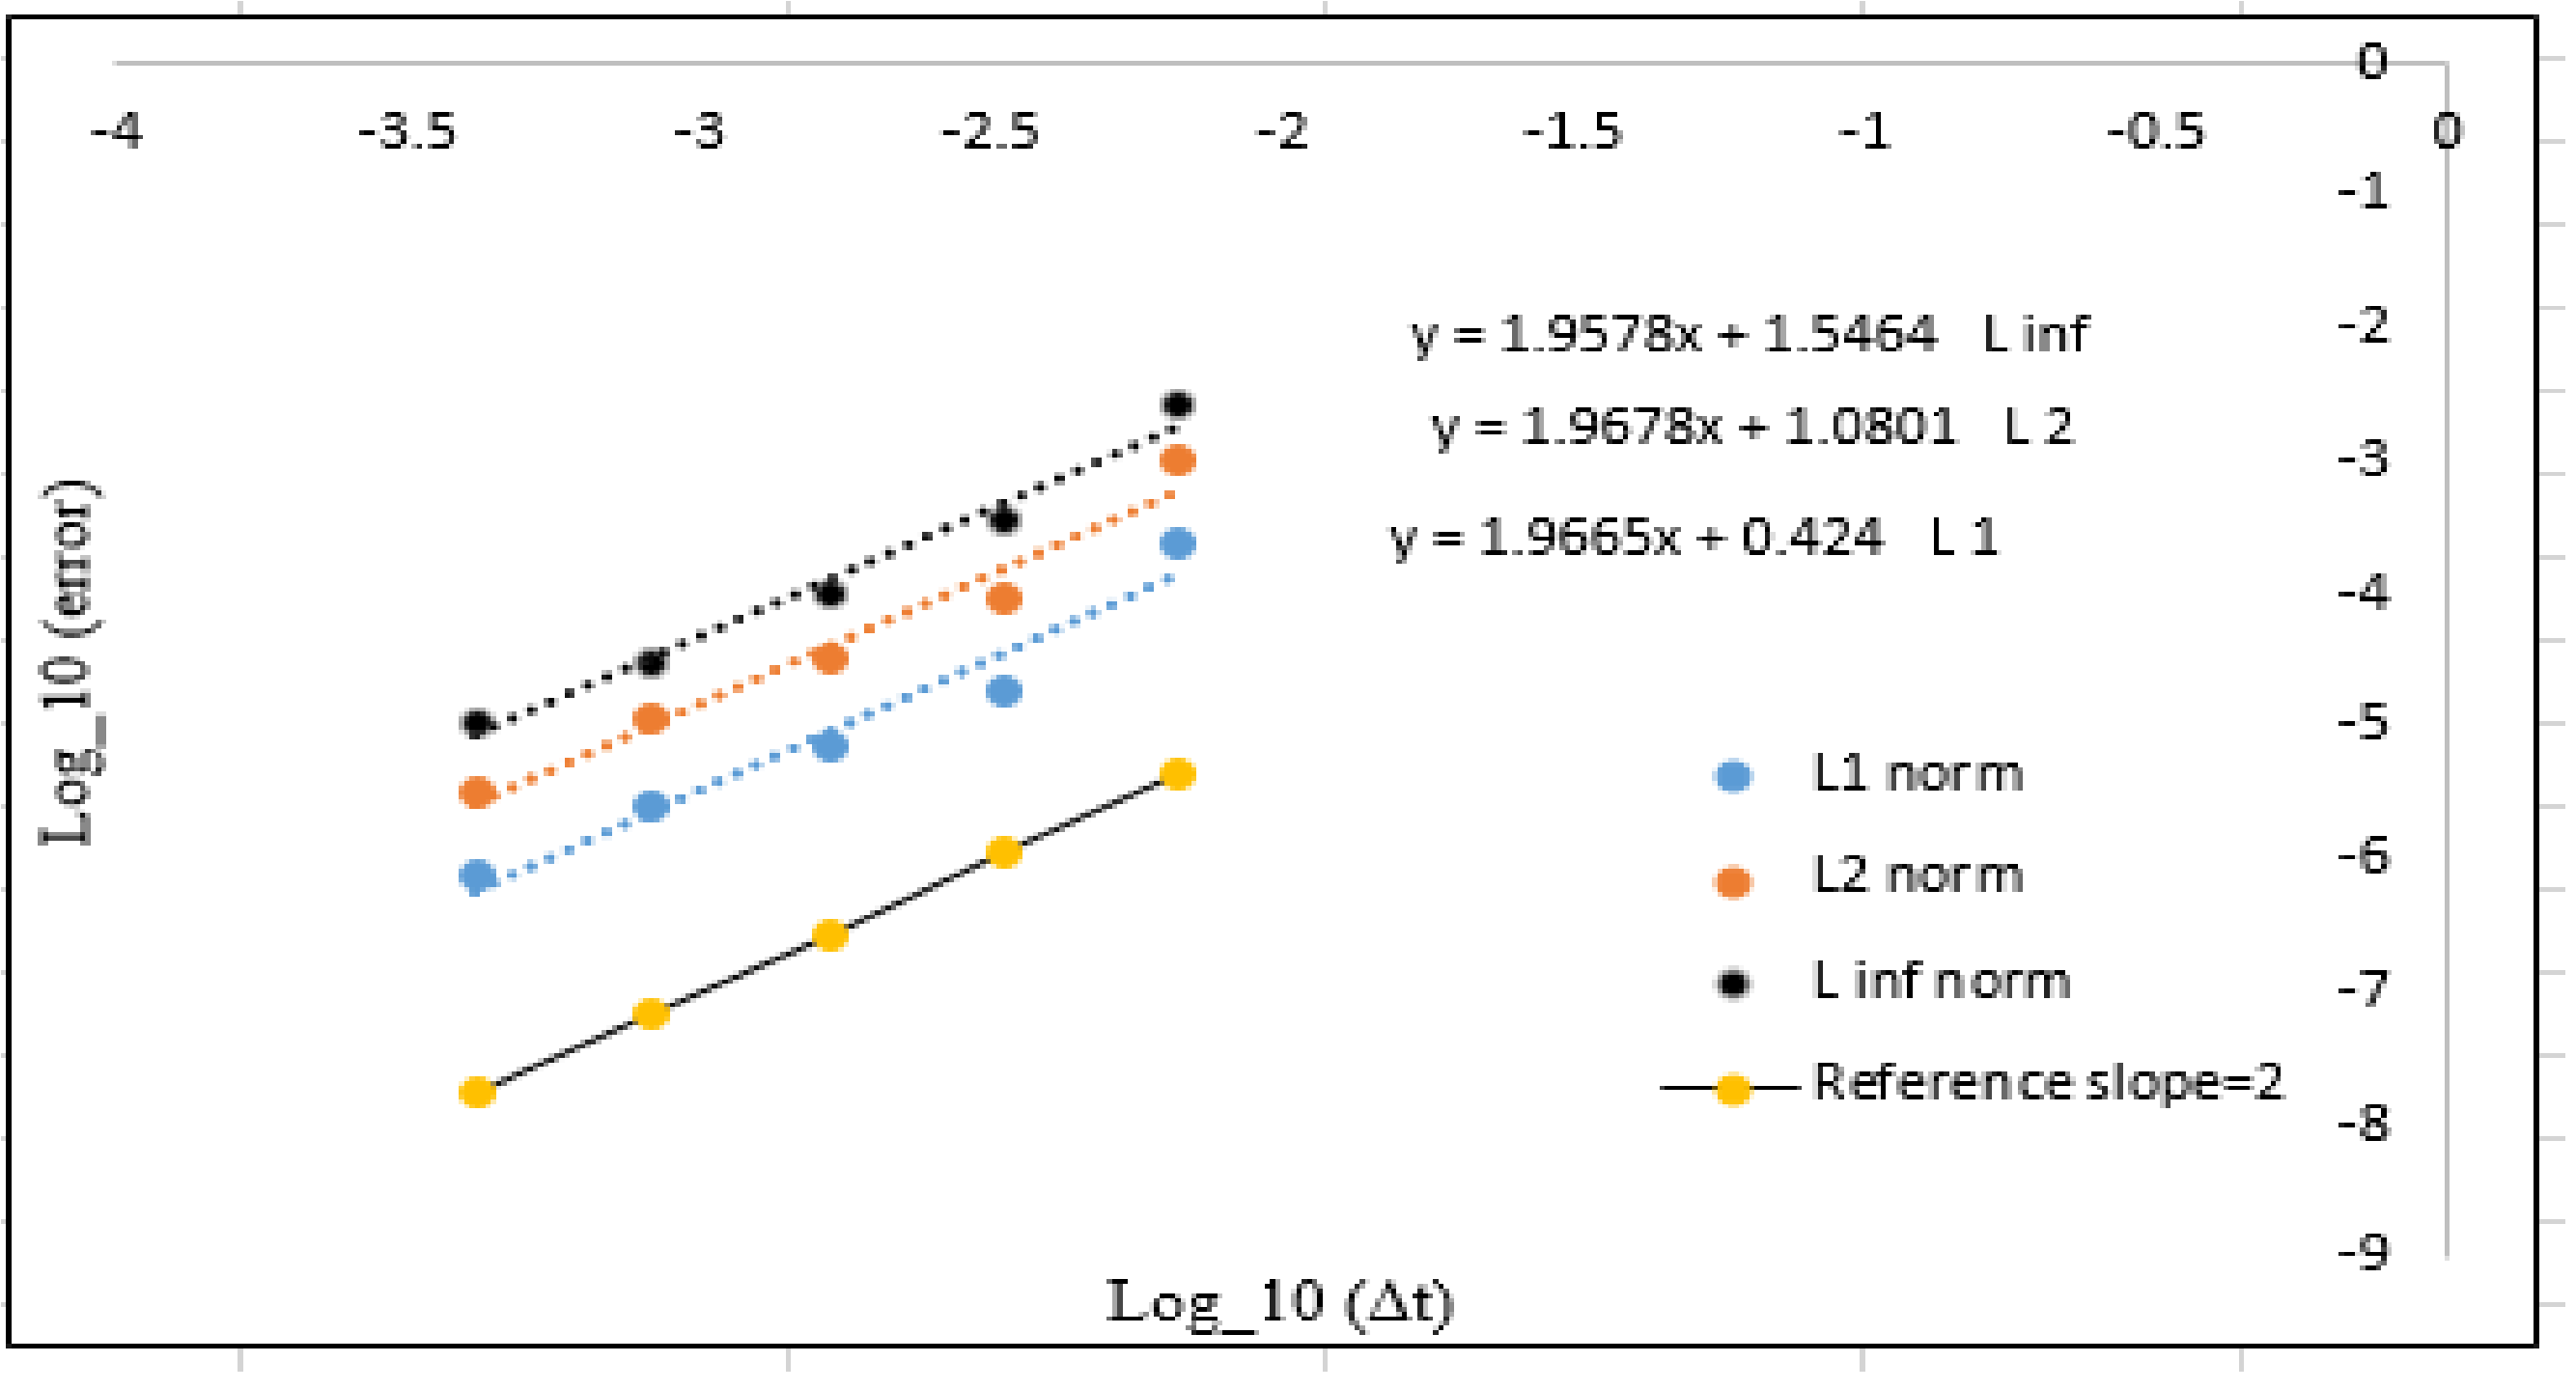
\includegraphics[width=4.5in]{C:/Users/HONGJI/Latex Home directory/Pm2_unf1_np_P_rate.jpg}
		\caption{Log-Log plot of Convergence rate for Pressure Alg 3. }\label{fig:6.19b}
	\end{subfigure}
	\quad
	\begin{subfigure}[t]{4.5in}
		\centering
		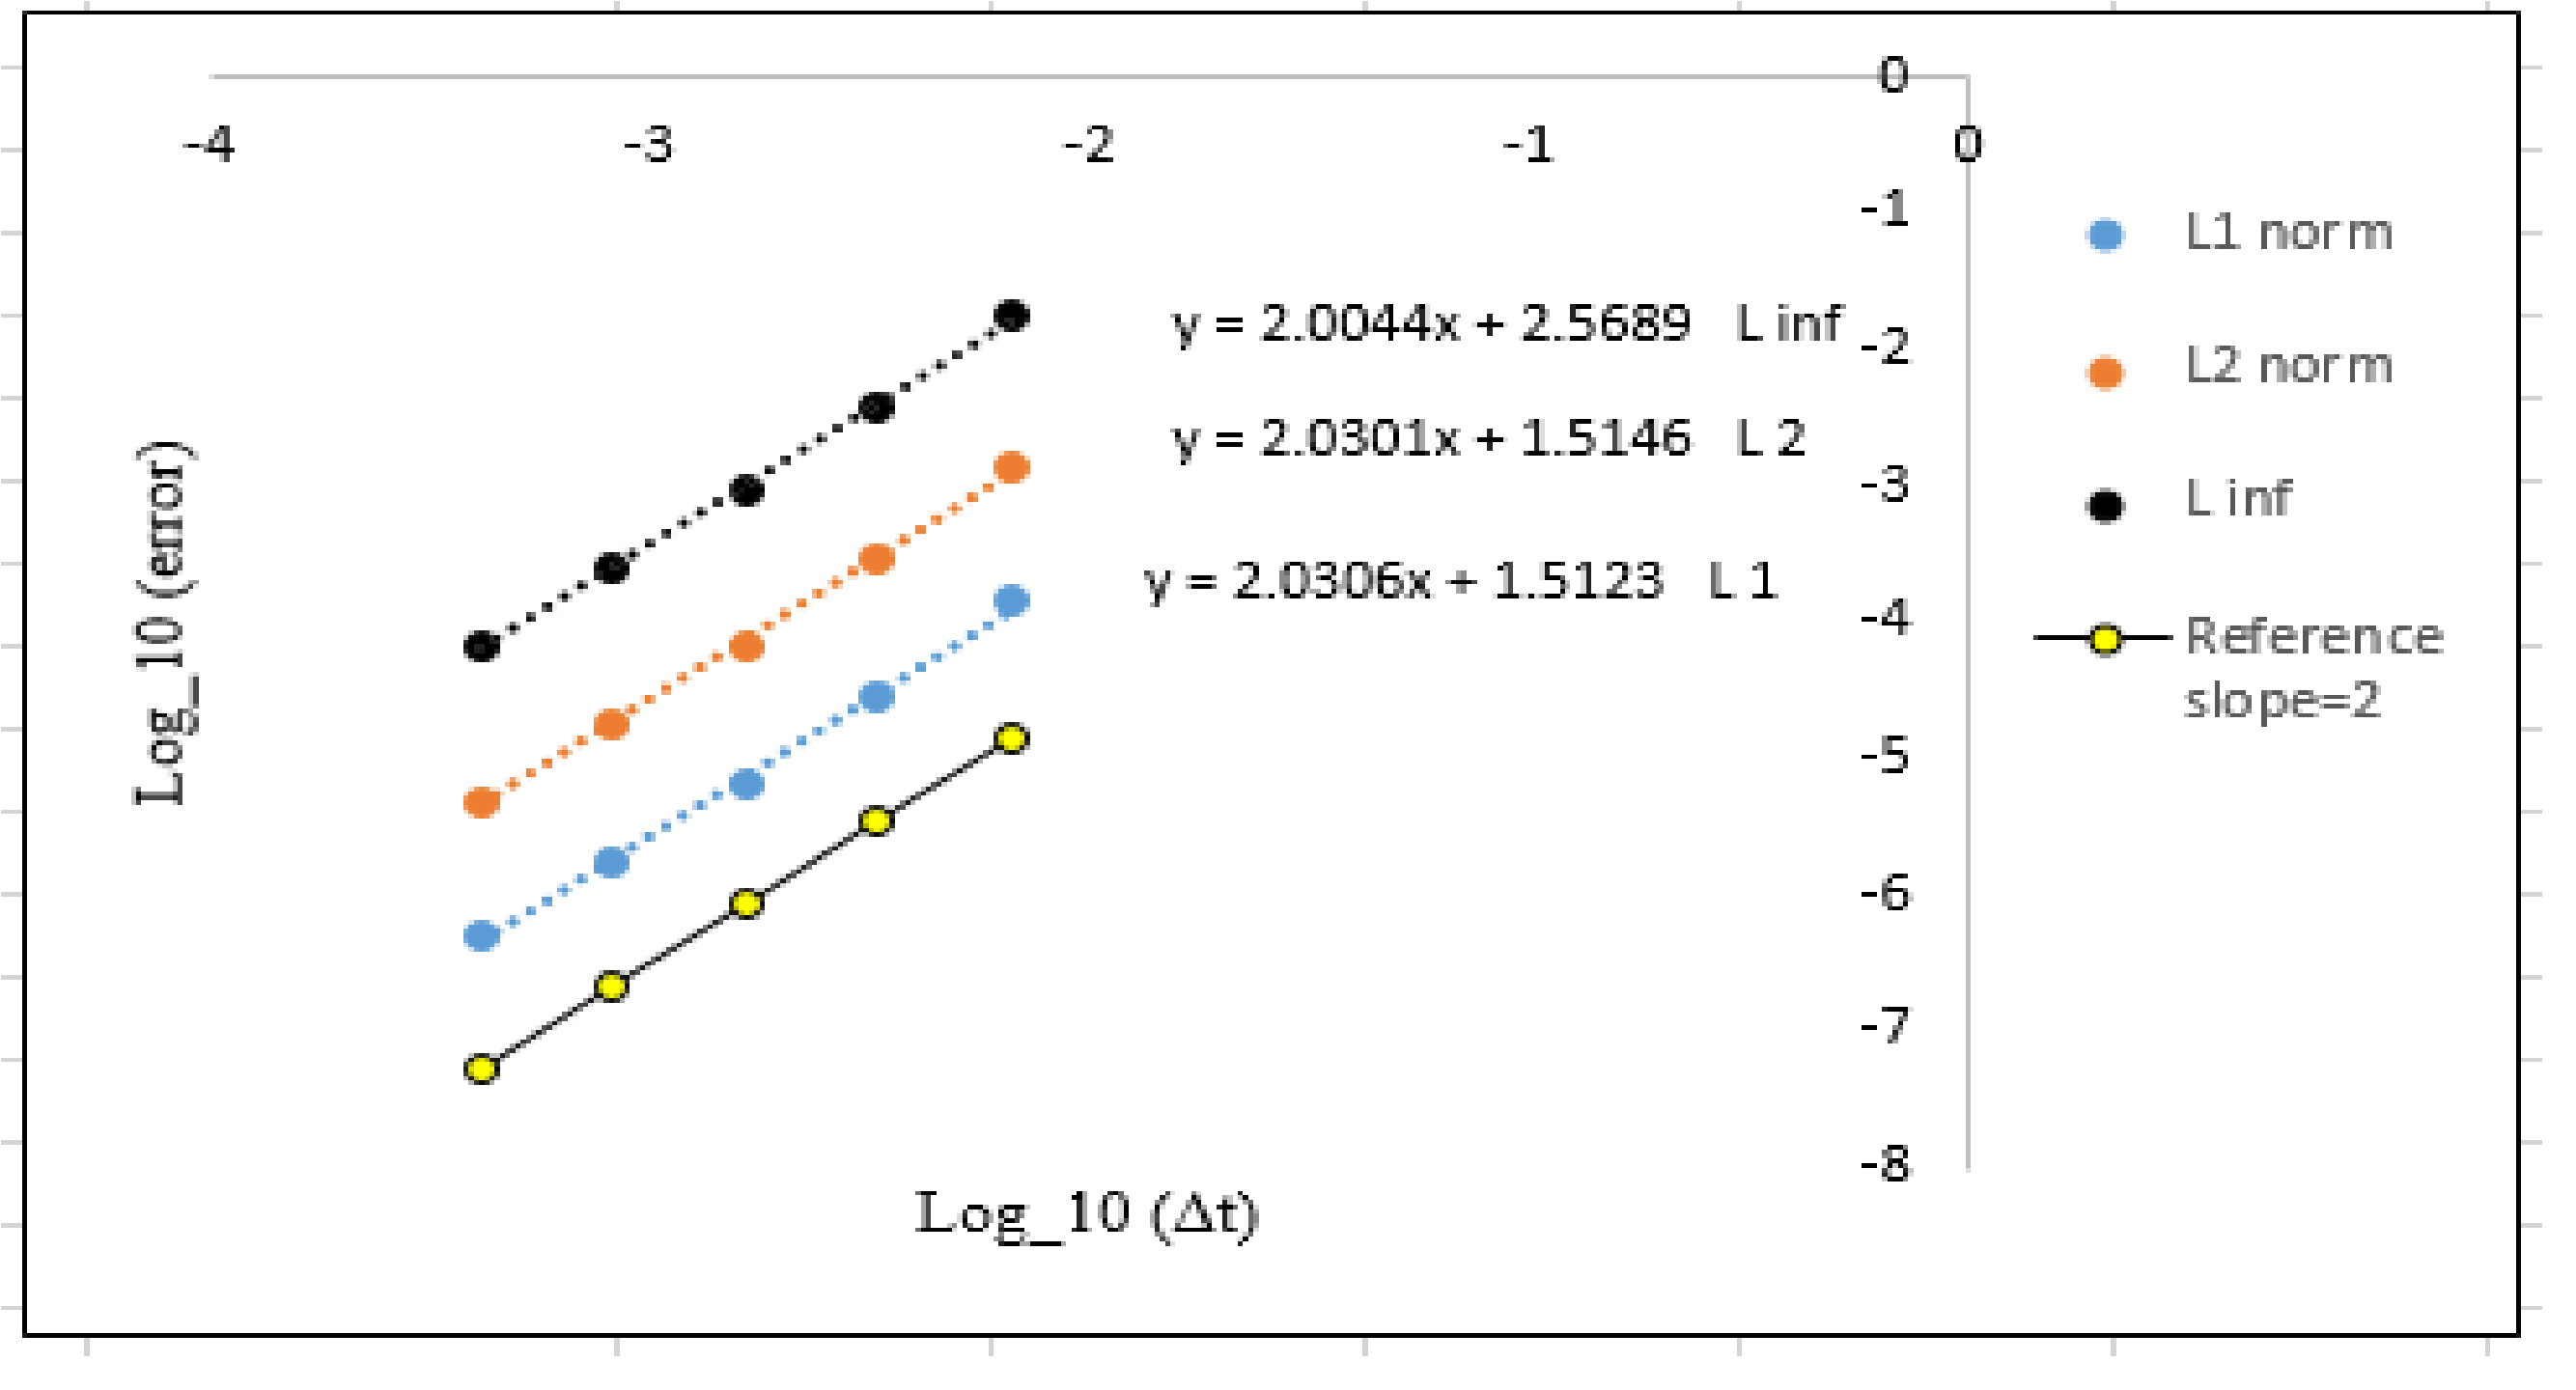
\includegraphics[width=4.5in]{C:/Users/HONGJI/Latex Home directory/Gauge_unf1_np_P_rate.jpg}
		\caption{Log-Log plot of Convergence rate for Pressure Gauge method }\label{fig:6.19b}
	\end{subfigure}
	\caption{Plot of Convergence rates for the Unforced flow problem with Normalised Pressure approach used. Domain: $[-\dfrac{\pi}{4}, \dfrac{\pi}{4}]^2$, time = 1 and CFL = 0.5. In each plot, the data points corresponding to grid sizes of 15, 30, 60, 120, 240.}\label{fig:6.16}
\end{figure}

\begin{figure}[H]
	\centering
	\begin{subfigure}[t]{2.2in}
		\centering
		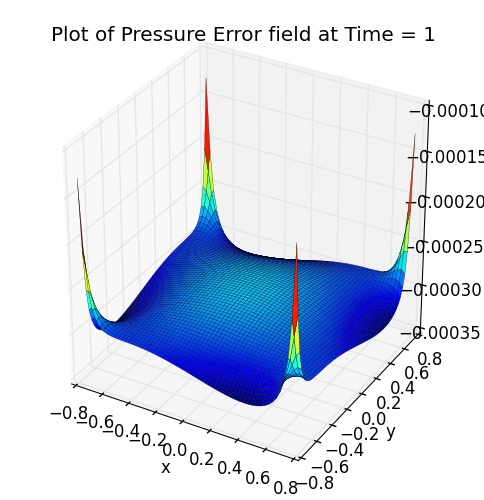
\includegraphics[width=2.2in]{C:/Users/HONGJI/Latex Home directory/Pm1b_unf1_np_P_error_t_1_grid_60.jpg}
		\caption{Pressure error field for Alg 2 method}\label{fig:6.19a}		
	\end{subfigure}
	\quad
	\begin{subfigure}[t]{2.6in}
		\centering
		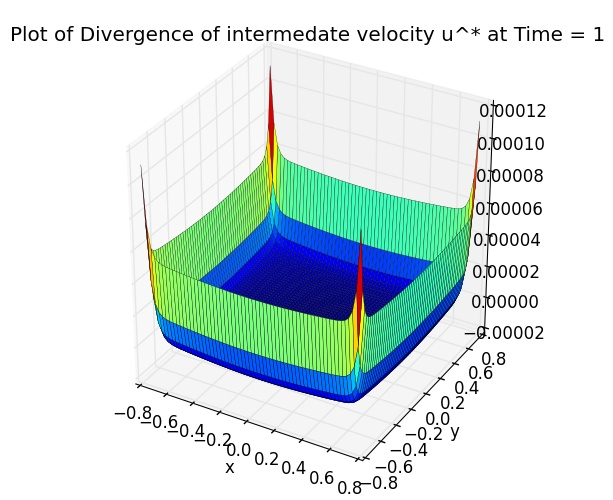
\includegraphics[width=2.6in]{C:/Users/HONGJI/Latex Home directory/Pm1b_unf1_np_div_uvstar_t_1_grid_60.jpg}
		\caption{Divergence of intermediate velocity field Alg 2}\label{fig:6.19b}
	\end{subfigure}
	\quad
	\centering
	\begin{subfigure}[t]{2.2in}
		\centering
		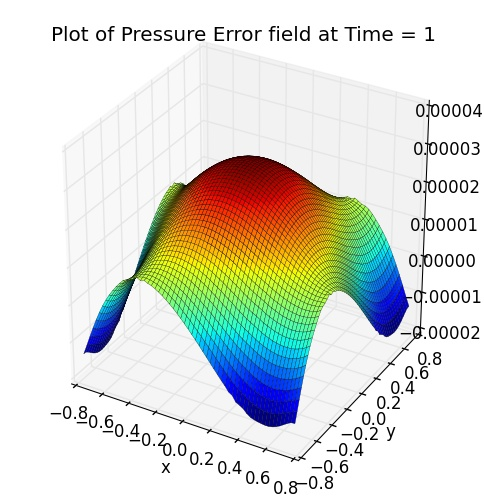
\includegraphics[width=2.2in]{C:/Users/HONGJI/Latex Home directory/Pm2_unf1_np_P_error_t_1_grid_60.jpg}
		\caption{Pressure error field for Alg 3 method}\label{fig:6.19a}		
	\end{subfigure}
	\quad
	\begin{subfigure}[t]{2.5in}
		\centering
		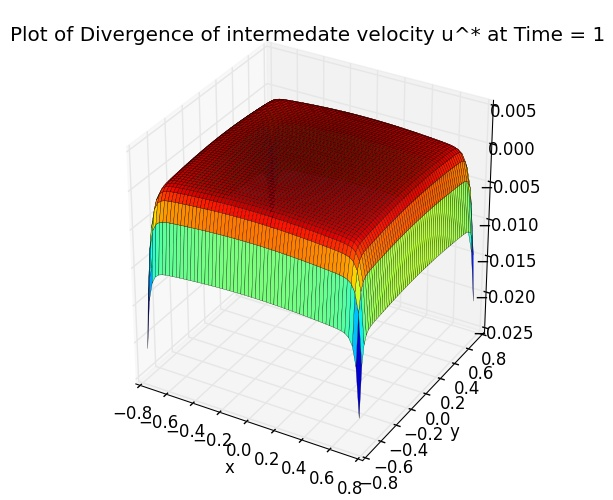
\includegraphics[width=2.5in]{C:/Users/HONGJI/Latex Home directory/Pm2_unf1_np_div_uvstar_t_1_grid_60.jpg}
		\caption{Divergence of intermediate velocity field Alg 3}\label{fig:6.19b}
	\end{subfigure}
	\quad
	\begin{subfigure}[t]{2.5in}
		\centering
		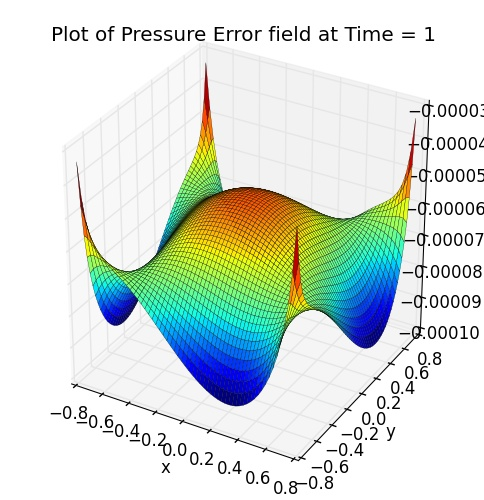
\includegraphics[width=2.5in]{C:/Users/HONGJI/Latex Home directory/Gauge_unf1_P_error_t_1_grid_60.jpg}
		\caption{Pressure error field Gauge method }\label{fig:6.19b}
	\end{subfigure}
	\caption{Plot of Pressure error fields for the Unforced flow problem with Normalised Pressure approach used. Domain: $[-\dfrac{\pi}{4}, \dfrac{\pi}{4}]^2$, time = 1 and CFL = 0.5.}\label{fig:6.16}
\end{figure}

To further investigate the cause of degradation in accuracy in Alg 2, recall in normal mode analysis, we showed that the choice of pressure approximation $q = p^{n-1/2}$ results contradicting normal pressure gradient along the boundary especially if the normal analytic pressure gradient is not zero. This is the case in this unforced flow problem. For instance, the normal pressure gradient at west boundary ($x=\dfrac{\pi}{4}$ at any time is: $\dfrac{1}{2}\left(-\sin(\dfrac{\pi}{4}\right)$ which is obviously not zero. Hence this means this choice of $q$ does not work properly at the boundary.\\

It is supported by the plot of normal pressure gradient at West boundary. The plot of numerical solution is different to that of the analytical solution. This is amplified at the 4 corners of the domain where large spikes occur. We therefore infer that it is the non-smoothness caused by the inconsistent pressure approximation which degrades the global convergence of Alg 2.\\

We now propose a simplified modification to solve the problem by defining $q$ to be $q = 2\phi^{n-1/2} - \phi^{n-3/2}$. This results in a second order accurate pressure approximation to $p^{n+1/2}$. This can be shown using a simple Taylor series argument. With this modified pressure approximation $q$, the numerical normal pressure gradient now approximates the analytic one better. It is converging to the analytic pressure gradient at higher than second order rate too. The non-smooth spikes are now eliminated which reduces the error and also lifts up the global pressure error convergence to 2.5 order.

\begin{figure}[H]
	\centering
	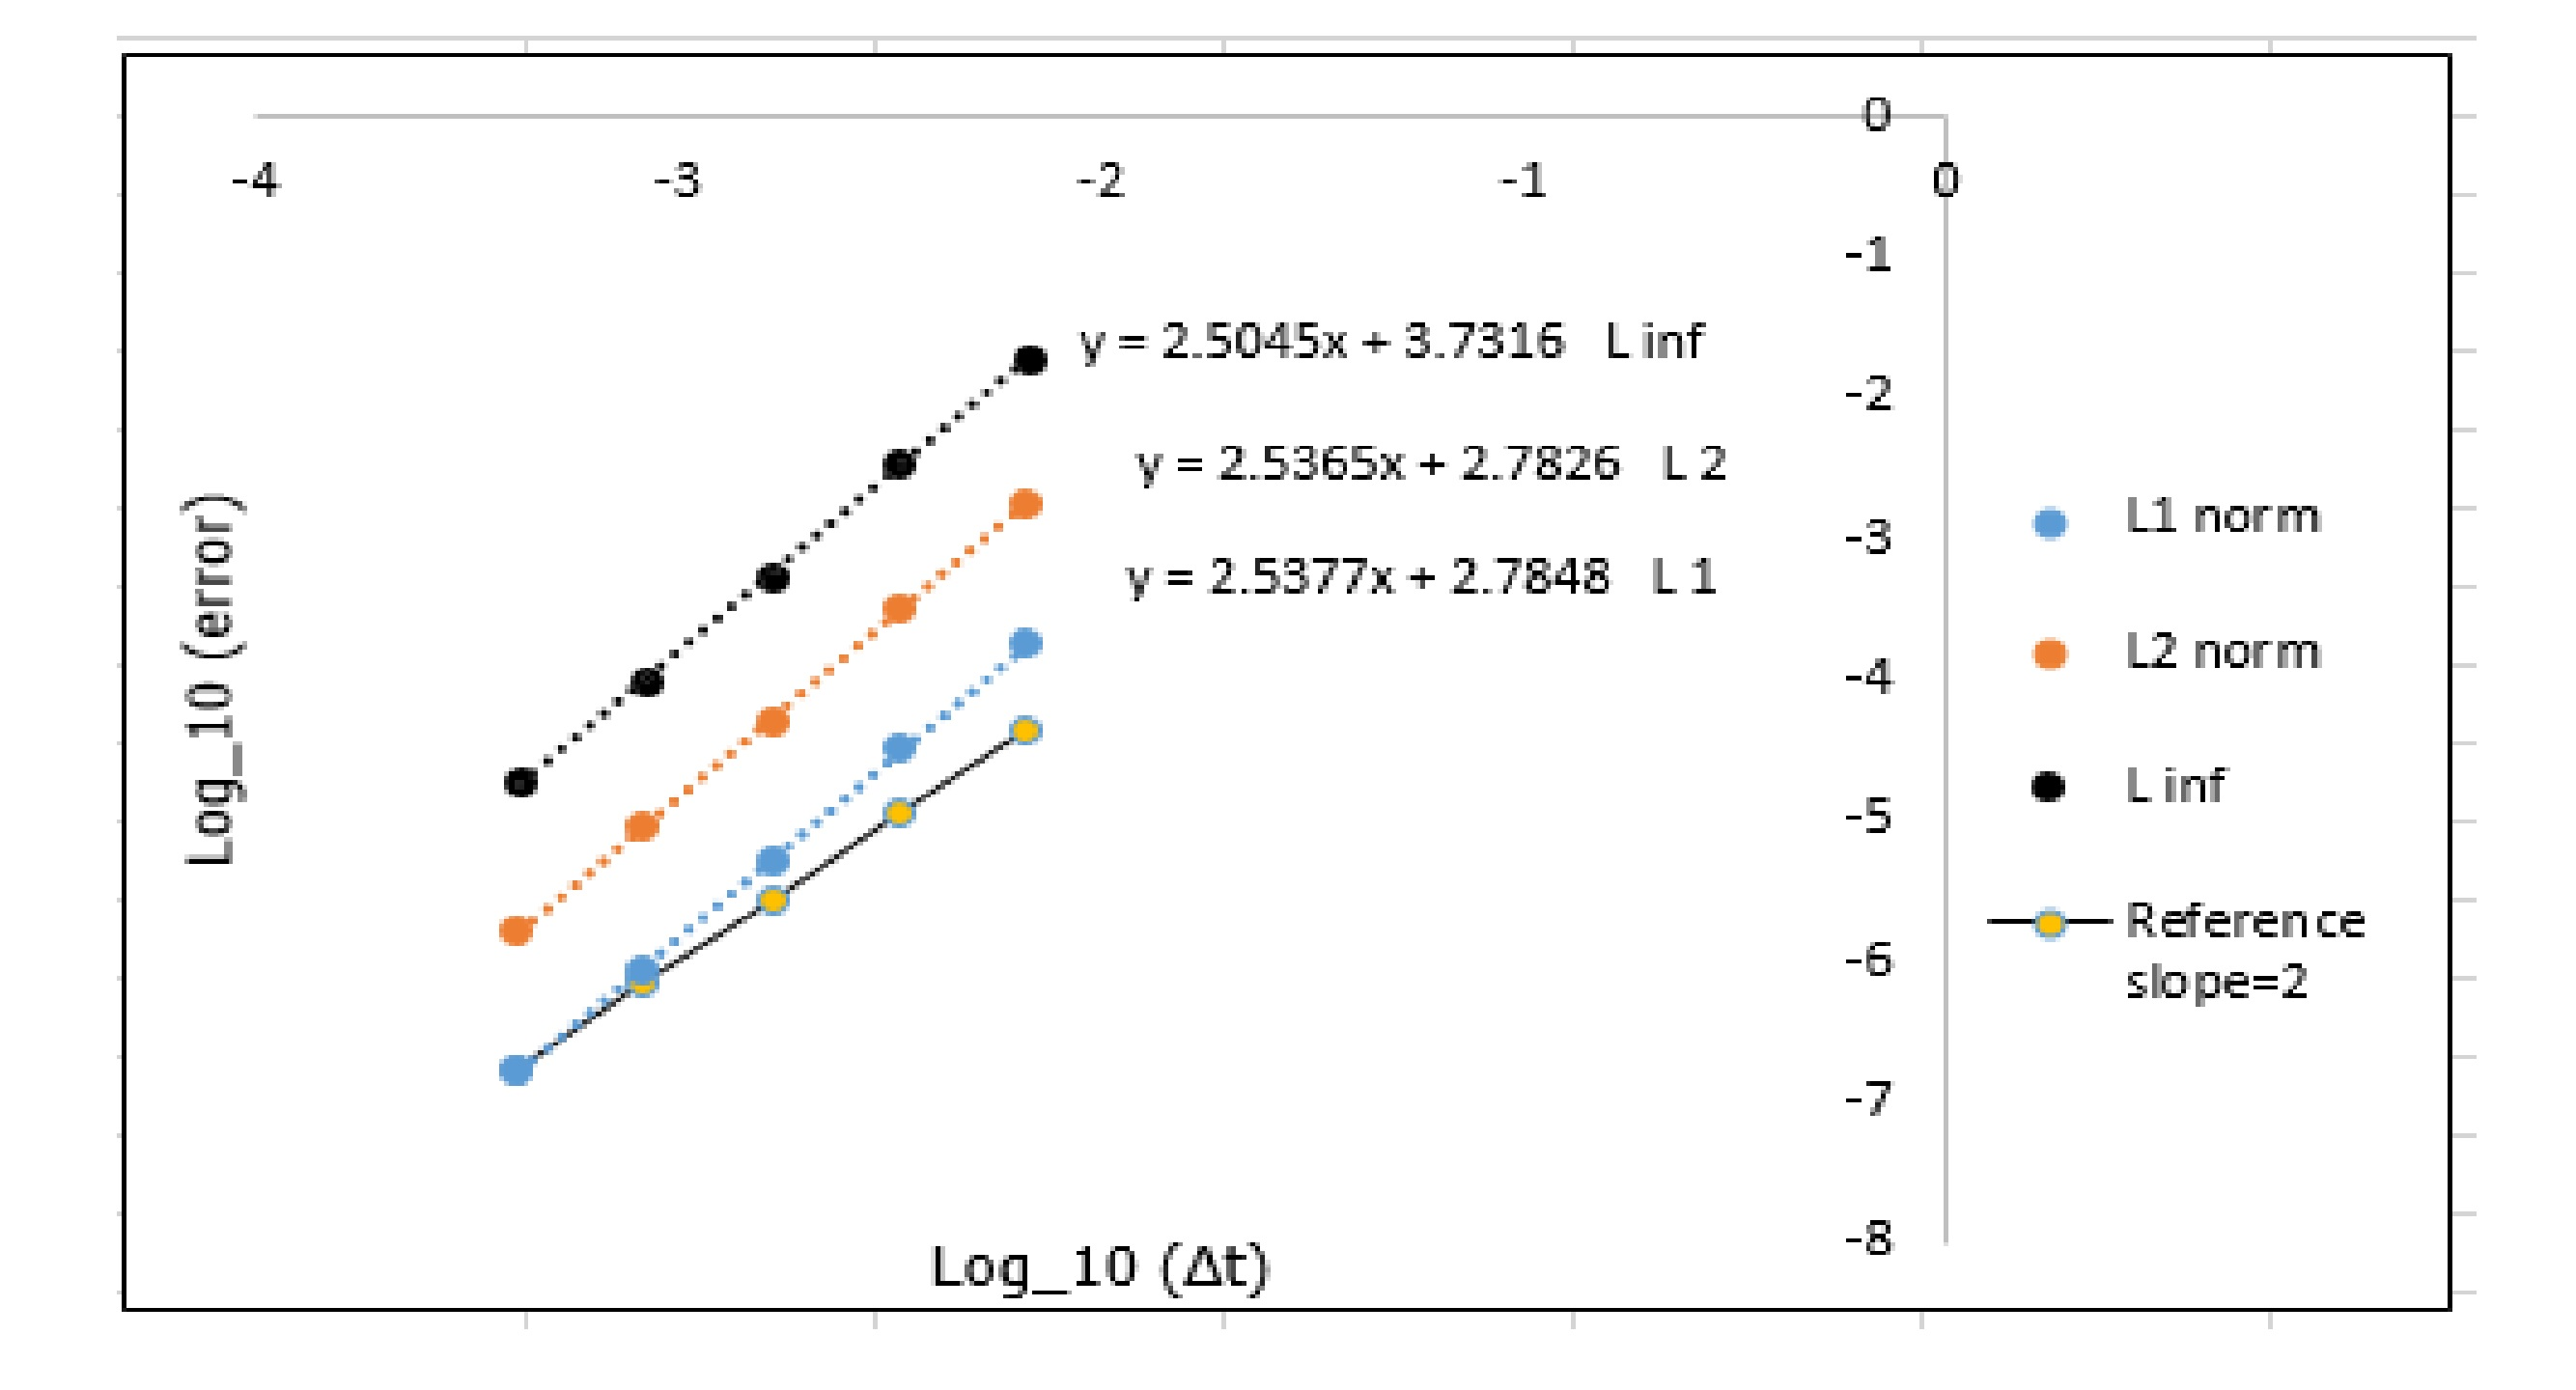
\includegraphics[width=4.5in]{C:/Users/HONGJI/Latex Home directory/Pm1b2_unf1_np_P_rate.jpg}
	\caption{Log - log plot of the pressure error convergence rate with the modified $q = 2\phi^{n-1/2} - \phi^{n-3/2}$ used }\label{fig:6.23}
\end{figure}

\begin{figure}[H]
	\centering
	\begin{subfigure}[t]{2.6in}
		\centering
		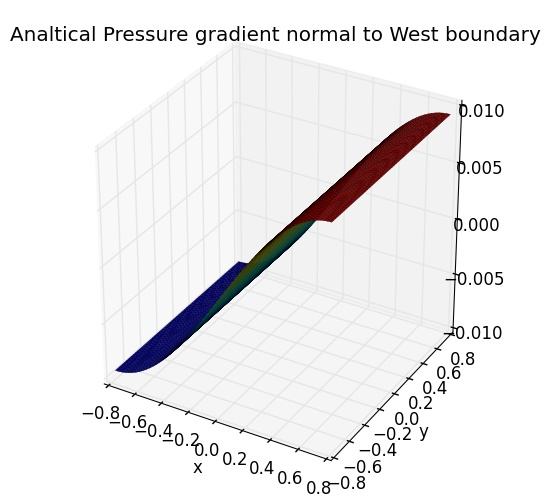
\includegraphics[width=2.6in]{C:/Users/HONGJI/Latex Home directory/Pm1b2_unf1_np_W_NPexgrad_t_1_grid_60.jpg}
		\caption{Plot of analytic pressure gradient normal to west boundary}\label{fig:6.19a}		
	\end{subfigure}
	\quad
	\begin{subfigure}[t]{2.2in}
		\centering
		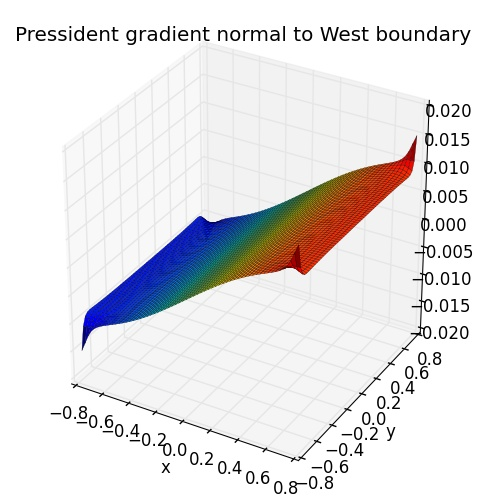
\includegraphics[width=2.2in]{C:/Users/HONGJI/Latex Home directory/Pm1b_unf1_np_W_Npf_t_1_grid_60.jpg}
		\caption{Plot of numerical pressure gradient normal to west boundary with $q = p^{n-1/2}$ is used}\label{fig:6.19b}
	\end{subfigure}
	\quad
	\centering
	\begin{subfigure}[t]{2.5in}
		\centering
		\includegraphics[width=2.5in]{C:/Users/HONGJI/Latex Home directory/Pm1b2_unf1_np_W_Npf_t_1_grid_60.jpg}
		\caption{Plot of numerical pressure gradient normal to west boundary with the modified $q = 2\phi^{n-1/2} - \phi^{n-3/2}$ used}\label{fig:6.19a}		
	\end{subfigure}
	\caption{Plot of normal pressure gradients and convergence rates for Alg 2 with modified $q = 2\phi^{n-1/2} - \phi^{n-3/2}$ used. Domain: $[-\dfrac{\pi}{4}, \dfrac{\pi}{4}]^2$, time = 1 and CFL = 0.5.}\label{fig:6.16}
\end{figure}


\newpage
\section{Driven cavity flow}
In this section, we consider a very interesting flow problem: the Lid-Driven cavity. Driven cavity flow has been well studied in the literature. It is a simple example to show the effect of Reynolds number and turbulent and unsteady flows. We mainly illustrate the qualitative findings here through numerical simulations. There are however benchmark results for $3D$ and $2D$ Lid-driven cavity problems for the purpose of comparing accuracy of numerical solvers.\\ (\textbf{citation, Goda, Shen...})\\

Although the problem set up could vary, however the essential idea is the same. We have a fluid initially at rest except at one boundary where either horizontal or vertical component has a constant non-zero velocity (i.e. 1). The flow in the interior is then driven by the non-zero velocity at the boundary. This is like opening the lid along the non-zero boundary and sliding it at a constant velocity. The flow pattern depend on the value of Reynolds numbers and with low to moderate Reynolds number (often below 10000) the flow can reach to steady state whereas for higher Reynolds numbers, turbulence will occur in which no steady state solutions can be obtained. In fact, turbulence only occur in 3-dimensional type of flows and hence our $2D$ numerical solver would not show the pattern completely. Nevertheless, as our result presents, as Reynolds number increases, the flow does become unsteady which is aligned with the turbulence behaviour in $3D$ simulations.

\subsection{Problem set up}
We consider a fluid confined in the square domain: $[0,1]^2$. The fluid velocities are initially zero except for $v$ at the East boundary ($x=1$) which it is equal to 1 (i.e. $v(x=1,y,0)=1$). The problem set up is illustrated in the diagram below. The full Navier Stokes equations of incompressible flow is used. We consider the flow at different Reynolds numbers ($R = 1000, 10000$). The Gauge method was used to compute the solutions with grid size $100 \times 100$ and $CFL = 0.5$. \\

\begin{figure}[H]
	\centering
	\includegraphics[width=5.5in]{C:/Users/HONGJI/Latex Home directory/Lid_driven_set_up.png}
	\caption{Problem setup of the Lid-driven cavity. The flow is driven by the constant vertical velocity along the East boundary ($v=1$ at $x=1$)  }	
\label{fig:6.16}
\end{figure}
First we consider moderate Reynolds number flows of with value of 1000, the fluid converges to the steady state after about a time of 20s. 3 main eddies are formed. The main one starts from the corner near the East boundary since the initial flow starts from here. It then slides to the middle over time forming a constant main vortex. Mean while two other smaller eddies are then formed one after another. The streamline plots are presented below illustrate the flow patterns.\\

\subsection{Results}
At higher Reynolds number the flow become unsteady (or ``turbulent") as more smaller unsteady eddies are formed. This is clearly shown by the streamline plot at Reynold = 10000. Hence our result is in line with the literature too.\\

\begin{figure}[H]
	\centering
	\begin{subfigure}[t]{2.5in}
		\centering
		\includegraphics[width=2.5in]{C:/Users/HONGJI/Latex Home directory/streamline_plot_t_0s_grid_100.pdf}
		\caption{Streamline plot of velocity fields at time 0s}\label{fig:6.19a}		
	\end{subfigure}
	\quad
	\begin{subfigure}[t]{2.5in}
		\centering
		\includegraphics[width=2.5in]{C:/Users/HONGJI/Latex Home directory/streamline_plot_t_ 20s_grid_100.pdf}
		\caption{Streamline plot of velocity fields at time 20s}\label{fig:6.19b}
	\end{subfigure}
	\caption{Streamline plot of velocity fields for driven cavity flow. $v(x=1,y,t) = 1$ with grid size 100 and CFL = 0.5 used.}\label{fig:6.16}
\end{figure}

Reynolds number = 10000
\begin{figure}[H]
	\centering
	\includegraphics[width=3.0in]{C:/Users/HONGJI/Latex Home directory/streamline_plot_t_20_grid30_Re_10000.pdf}
	\caption{Streamline plot of velocity fields at time 20s with Reynolds number equal to 10000}\label{fig:6.19}		
\label{fig:6.16}
\end{figure}

Plots of velocity and pressure solutions are also shown below:
\begin{figure}[H]
	\centering
	\begin{subfigure}[t]{2.5in}
		\centering
		\includegraphics[width=2.5in]{C:/Users/HONGJI/Latex Home directory/Gauge_dcv_uf_grid_120.jpg}
		\caption{Plot of $U$ velocity at time 20s}\label{fig:6.19a}		
	\end{subfigure}
	\quad
	\begin{subfigure}[t]{2.5in}
		\centering
		\includegraphics[width=2.5in]{C:/Users/HONGJI/Latex Home directory/Gauge_dcv_vf_grid_120.jpg}
		\caption{Plot of $V$ velocity at time 20s}\label{fig:6.19b}
	\end{subfigure}
	\quad
	\centering
	\begin{subfigure}[t]{3.5in}
		\centering
		\includegraphics[width=2.5in]{C:/Users/HONGJI/Latex Home directory/Gauge_dcv_pf_grid_120.jpg}
		\caption{Plot of Pressure at time 20s}\label{fig:6.19a}		
	\end{subfigure}
	\caption{Plot of velocity and pressure solutions for driven cavity problem with Reynolds number equal to 1000. The East boundary for $V$ velocity is kept to be 1 over time. Grid size of 100 and CFL = 0.5 was used.}\label{fig:6.16}
\end{figure}

Although our result shows the unsteady pattern of flow as Reynolds number increases which is in line with the literature in general \textbf{Citation}, however to examine the turbulent behaviour we should implement $3D$ numerical solvers. This could be a further investigation in the future. Once again this section is only aimed to be a qualitative illustration of the classic Lid-driven cavity problem. 
  
\chapter{Conclusions}
\label{chapter8}
In this thesis, we have examined robust Projection method to the numerical solutions of Incompressible Navier Stokes equations. We have talked about the origin of the method which is based on the idea of Helmholtz Hodge decomposition theorem. We have described the Chorin's original method and the second order extensions as well as the Gauge method. We have analysed these methods' accuracy through normal mode analysis. In a periodic channel domain,(following Brown's analysis) our normal mode analysis is predicting second order accuracy for all projection methods. This is also consistent with our numerical results. However further analysis could be done in a more general domain because normal mode analysis is restricted on the domain we work with and the error convergence might behave differently too \cite{pyo2005normal}. 

In summary:
\paragraph*{We observe that the Gauge method} shows fully 2nd order convergence in Pressure in all examples and domains considered whereas Projection methods show a degraded accuracy in some examples (see Unforced flow example in Results chapter). 
We observe that the Projection methods depends strongly on the smooth of domain (especially for Alg 2 with a lagged pressure approximation used). The exact cause of this problem still remains open (\cite{guermond2004error}). This finding is consistent with Shen et.al where they have bounded the $L_2$ norm of Pressure error to be only 1.5 order accurate in general domains (e.g. the square domain with Dirichlet boundary conditions we have considered in the Forced flow example). For details of the proof see \cite{guermond2004error, pyo2005normal}. In the case of periodic channel, all projection methods show 2nd order accuracy in pressure. This is consistent with the predications of error estimates by our normal mode analysis done in previous chapter where a periodic channel domain was considered. 

\paragraph*{Necessity for accurate boundary condition} of the tangential component of the intermediate velocity field ($\textbf{u}^*$).
We have observed that second order approximation $\phi^{n+1}$ is needed when computing $\textbf{$\tau$}\cdot\textbf{u}^*$ in the projection step. This is consistent with our normal mode analysis predications and findings of other researchers too \cite{brown2001accurate}.

\paragraph*{Modification to pressure approximation in Alg 2}
We have observed that the inconsistent normal pressure gradient in Alg 2 is caused by an inappropriate choice of pressure approximation $q$ used. This introduces non-smooth along the boundary of pressure gradients. This is more evident when the test problems have non-zero pressure gradients. However with a modified $q = 2\phi^{n-1/2} - \phi^{n-3/2}$, we restore fully second order convergence in pressure. The exact reason of this improvement however still subject to more careful considerations.

\paragraph*{Further research} could be looking at flow in general domain and complex geometry, Interface problems. Finite element could also to be used too. We are also interested in higher order schemes e.g. 4th 6th order schemes using compact finite difference.
  %etc




% APPENDICES


  % change chapter name and counters (eg Chapter 1 -> Appendix A)
  \appendix


  % assuming there are files appendix1.tex etc...
  %
\chapter{Error analysis for first order Projection Methods}
\label{appendix1}

\newpage

\section{Error analysis on Chorin's original projection method}

\subsection{Notation and Preliminaries}
\begin{itemize}
\item Functional spaces
\end{itemize}
1. $\textit{L}^p$ space\\
A space of $p$th power integrable functions. (space for which the p-th power of the absolute value is Lebesgue integrable). $\textbf{should I give a very precise and formal definition?}$\\

2. Sobolev space\\
A subspace of $\textit{L}^p$ in which the functions contained has the property that its weak derivatives up to kth order has finite $\textit{L}^p$ norm.
\begin{equation}
||f||_{k,p} = (\sum^k_{i=0} \int_{\Omega} |f^{(i)} (x)|^p dx)^{\dfrac{1}{p}} 
\end{equation}

In this case we are concerned with the $\textit{L}^2 (\Omega) $ space (space of square integrable functions on bounded regular domain $\Omega \subset \mathbb{R}^d$ where $d=1,2,3$) and Sobolev space up to derivative one ($\textit{H}^1 (\Omega)$).\\
Hence we have the following norms:
%\begin{dgroup}
%\intertext{$\textit{•}^2$ space norm
%\begin{dmath}



  %\include{appendix2}
  %\include{appendix3}
  %etc




% BIBLIOGRAPHY


  % add Bibliography to table of contents
  \addcontentsline{toc}{chapter}{Bibliography}


  % list BibTeX (.bib) files and choose bibliography style
  \bibliography{references}
  \bibliographystyle{abbrv}

  % OR... do it manually in the file bibliography.tex
  %
\begin{thebibliography}{88} % assuming between 10 and 99 references

 \bibitem{chorin1968numerical} Chorin, Alexandre Joel. "Numerical solution of the Navier-Stokes equations." Mathematics of computation 22.104 (1968): 745-762.

 \bibitem{key2} Chorin, Alexandre Joel, and Jerrold E. Marsden. A mathematical introduction to fluid mechanics. Vol. 3. New York: Springer, 1990.

 \bibitem{key3} Brown, David L., Ricardo Cortez, and Michael L. Minion. "Accurate projection methods for the incompressible Navier–Stokes equations." Journal of Computational Physics 168.2 (2001): 464-499.

 \bibitem{key4} A. S. Almgren, J. B. Bell, and W. G. Szymczak, A numerical method for the incompressible Navier–Stokes equations based on an approximate projection, SIAM J. Sci. Comput. 17(2), (1996).

 \bibitem{key5} A. S. Almgren, J. B. Bell, and W. Y. Crutchfield, Approximate projection methods. 1. Inviscid analysis, SIAM J. Sci. Comput. 22(4), (2000).

 \bibitem{key6} Temam, Roger. Navier-Stokes equations and nonlinear functional analysis. Vol. 66. Siam, 1995.
 
 \bibitem{key7} Maria Denaro, Filippo. "On the application of the Helmholtz–Hodge decomposition in projection methods for incompressible flows with general boundary conditions." International Journal for Numerical Methods in Fluids 43.1 (2003): 43-69.

 \bibitem{key8} Johnston, Hans, and Jian-Guo Liu. ``Finite difference schemes for incompressible flow based on local pressure boundary conditions.'' Journal of Computational Physics 180.1 (2002): 120-154.

 \bibitem{key9} 

 \bibitem{key10} 
 
 \bibitem{key11} Harlow, Francis H., and J. Eddie Welch. "Numerical calculation of time-dependent viscous incompressible flow of fluid with free surface." Physics of fluids 8.12 (1965): 2182.

 \bibitem{key12} Howell, Louis H., and John B. Bell. "An adaptive mesh projection method for viscous incompressible flow." SIAM Journal on Scientific Computing 18.4 (1997): 996-1013.

 \bibitem{key13} Bell, John B., Phillip Colella, and Harland M. Glaz. "A second-order projection method for the incompressible Navier-Stokes equations." Journal of Computational Physics 85.2 (1989): 257-283.

 \bibitem{key14} Kim, John, and Parviz Moin. "Application of a fractional-step method to incompressible Navier-Stokes equations." Journal of computational physics 59.2 (1985): 308-323.

 \bibitem{key15} R. Temam, Sur l’approximation de la solution des e´quations de Navier–Stokes par la me´thode des pas fractionnaires ii, Arch. Ration. Mech. Anal. 33 (1969) 377–385.
 
 \bibitem{key16} J. Shen, On error estimates of the projection methods for the Navier–Stokes equations: first-order schemes, SIAM J. Numer. Anal. 29 (1992) 57–77.
 
 \bibitem{key17} Fujita, Hiroshi, and Tosio Kato. "On the Navier-Stokes initial value problem. I." Archive for rational mechanics and analysis 16.4 (1964): 269-315.
 
 \bibitem{key18} Lal, Mindy Fruchtman, Mindy Frucbtman Lai, and Mindy Fruchtman. "~. A Projection Method for Reacting Flow in the Zero Mach Number Limit." (1993).
 
 \bibitem{key19} Minion, Michael L. "A projection method for locally refined grids." Journal of Computational Physics 127.1 (1996): 158-178.
 
 \bibitem{key20} Rannacher, Rolf. On Chorin's projection method for the incompressible Navier-Stokes equations. Springer Berlin Heidelberg, 1992.
 
 \bibitem{key21} R. Temam, Remark on the pressure boundary condition for the projection method, Theoret. Comput. Fluid Dynam. 3, 181 (1991).
 
 \bibitem{key22} W. E and J. Guo Liu, Projection method II. Godunov–Ryabenki analysis, SIAM J. Numer. Anal. 33, 1597 (1996).
 
 \bibitem{key23} J. Shen, On error estimates of the projection methods for the Navier–Stokes equations: Second-order schemes, Math. Comput. 65, 1039 (1996).
 
\end{thebibliography}



\end{document}
